%==============================================================================
% TEMPLATE FOR THESIS WAGENINGEN UNIVERSITY
% CREATED BY AREND LIGTENBERG JUNE 2006;
% EDITED BY KIM CALDERS 2014;
% EDITED BY BEN DEVRIES 2015;
% EDITED BY LOIC DUTRIEUX 2016;
% EDITED BY BENJAMIN BREDE 2019;
%==============================================================================

\documentclass [a4paper,12pt,twoside]{book}
\usepackage[utf8]{inputenc}
\usepackage[dutch,english]{babel}
\usepackage{graphicx}
%\usepackage{natbib} % replaced by biblatex
\usepackage{amsmath}
\usepackage{fancyhdr}
\usepackage[small,bf]{caption}
%\captionsetup[table]{skip=10pt}
\usepackage{multirow}
%\usepackage[body={6.0in, 8.2in},left=1.50in,right=1.50in]{geometry} %% very narrow
\usepackage[top=3.35cm, bottom=3.35cm, left=2.5cm, right=2.5cm]{geometry}
\usepackage[parfill]{parskip}
%\usepackage{enumitem} % replaced by enumitem
%\usepackage[rightcaption]{sidecap}
%\usepackage{epstopdf}
\usepackage{pdfpages}
%\usepackage[hidelinks]{hyperref} % see later
\usepackage{color}
\usepackage{appendix}

% extra packages added by Ben
\usepackage{rotating} % for rotating figures
\usepackage{changepage} % for indenting entire paragraphs
\usepackage{float} % help with table positioning
\floatstyle{plaintop} % caption on top
\restylefloat{table} % see above. Use: \begin{table}[H]
%\usepackage{textcomp} % \textdegree
%\usepackage{fixltx2e} % for the \textsubscript command outside of a math environment
\usepackage{csquotes} % for block quotes, use {displayquote} environment
\usepackage{todonotes}
%\usepackage{soul}
\usepackage{fp}
\usepackage{tabularx}
%\usepackage{subcaption}
\usepackage{pdflscape}
%\usepackage{gensymb}
%\usepackage{mhchem}
%\usepackage{wrapfig}

% extra packages added by Ben B
\usepackage{booktabs} 
\usepackage{microtype} % fancy typesetting
\usepackage[plain]{fancyref} % fancy cross-references
\usepackage{enumitem} % flexible numeration/list environments
\usepackage{pageslts} % to get total number of pages for frontmatter
\usepackage{etoolbox} % to fix acronym macro

% Extra packages added by Martijn W
\usepackage{algorithm,algpseudocode}

% make \url{} command available in text, break urls at hyphens (important for bibliography)
\PassOptionsToPackage{hyphens}{url}
\usepackage[bookmarksdepth=2,colorlinks=false,hidelinks]{hyperref}
\usepackage{url}

% bibliography with biblatex
\usepackage[
	backend=biber,
	natbib, % allow natbib cite commands
	alldates=year,
	style=numeric,
	sorting=nyt, % sorting order of the bibs: name, year, title
	sortcites, % sort in cite, when multiple refs are cited
	giveninits, % abbreveate first names
	maxbibnames=100, % max names per biobliography entry
	minbibnames=13,
	maxcitenames=2, % max names per citation
	uniquelist=false, % force inline citations to have no first names or additional co-authors
	uniquename=false, % force inline citations to have no first names or additional co-authors
	hyperref=false,
	doi,
	isbn=false
]{biblatex}

% add bib databases and give them unique labels to later refer to them
% paths can be absolute
% published papers of the PhD should be in both refs (or refsAdditional) and mypubs
\addbibresource[label=refs]{refs.bib}
\addbibresource[label=refsAdditional]{moreRefs.bib}
% use author+an field in ownPublications.bib to specify which author should be highlighted
\addbibresource[label=mypubs]{ownPublications.bib}

% biblatex + Mendeley: ignore some fields produced by Mendeley that are not biblatex conform (or not necessary)
\DeclareSourcemap{
	\maps[datatype=bibtex, overwrite]{
		\map{
			\perdatasource{refs}
			\step[fieldset=ISBN, null]
			\step[fieldset=month, null]
			\step[fieldset=abstract, null]
			\step[fieldset=file, null]
			\step[fieldset=keywords, null]
			\step[fieldset={mendeley-tags}, null]
			\step[fieldset=number, null]
		}
		\map{
			\perdatasource{refsAdditional}
			\step[fieldset=ISBN, null]
			\step[fieldset=month, null]
			\step[fieldset=abstract, null]
			\step[fieldset=file, null]
			\step[fieldset=keywords, null]
			\step[fieldset={mendeley-tags}, null]
			\step[fieldset=number, null]
		}
		\map{
			\pernottype{manual}
			\step[fieldset=url, null] % remove urls from all but manual > DOI has same information content
		}
	}
}

% add space between bibliography items
\setlength\bibitemsep{0.25\baselineskip}

% use all authors for fullcite
\preto\fullcite{\AtNextCite{\defcounter{maxnames}{99}}} 
%https://tex.stackexchange.com/questions/126226/how-do-i-instruct-fullcite-to-use-maxbibnames-rather-than-maxcitenames

% for biblatex + own publication list: make author name bold if annotated (bibtex field author+an in mypubs.bib)
\renewcommand*{\mkbibnamegiven}[1]{%
	\ifitemannotation{highlight}
	{\textbf{#1}}
	{#1}
}
\renewcommand*{\mkbibnamefamily}[1]{%
	\ifitemannotation{highlight}
	{\textbf{#1}}
	{#1}
}

% in bibliography: remove "in:" before journal names for articles
\renewbibmacro{in:}{%
	\ifentrytype{article}{}{\printtext{\bibstring{in}\intitlepunct}}
}

% in bibliography: removes pagination (p./pp.) before page numbers
\DeclareFieldFormat{pages}{#1}


% typeset units correctly
\usepackage{siunitx} 
\sisetup{range-units=single}
\DeclareSIUnit \lai{ \square\metre\per\square\metre }

\usepackage[labelformat=simple]{subcaption}
\renewcommand\thesubfigure{\alph{subfigure}}
\DeclareCaptionLabelFormat{subcaptionlabel}{\normalfont(\textbf{#2}\normalfont)}
\captionsetup[subfigure]{labelformat=subcaptionlabel}

% full acronyms once, then abbreviations
\usepackage{acronym} 



%\addto\captionsenglish{\renewcommand{\bibname}{References}} % REFERENCES > References

\widowpenalty10000
\clubpenalty10000

% allow up to 80% of page to be float (figure/table) and still print text
\renewcommand{\floatpagefraction}{.8}

\definecolor{Red}{rgb}{0.5,0,0}
\definecolor{Blue}{rgb}{0,0,0.5}


%=======================================================================
% GENERAL SETTINGS
%=======================================================================
%\oddsidemargin 40pt
%\evensidemargin 40pt
\setlength{\captionmargin}{5pt}
%\setlength{\textfloatsep}{10pt plus 1.0pt minus 2.0pt}
%\usepackage{pifont}
%\usepackage{times}
%\usepackage{txfonts}
%\usepackage[sc]{mathpazo}
%\usepackage{setspace}

\linespread{1.1} %1 is single spacing, 1.3 is oneandhalf spacing


%\citationstyle{dcu}
\sloppy
\setcounter{tocdepth}{0}

%% for internal use
\newcommand{\fixme}[1]{\emph{\marginpar{FIXME} (#1)}}
\newcommand{\readme}[1]{\emph{\marginpar{README} (#1)}}
\newcommand{\verifyme}[1]{\emph{\marginpar{VERIFYME} (#1)}}


%=======================================================================
% DEFINITION OF THE FANCY HEADERS
%=======================================================================
\pagestyle{fancy}
\renewcommand{\chaptermark}[1]{\markboth{#1}{}}
\renewcommand{\sectionmark}[1]{\markright{\thesection\ #1}}
\fancyhf{}
\fancyhead[LE,RO]{\bfseries\thepage}
\fancyhead[LO]{\bfseries\nouppercase{\rightmark}}
\fancyhead[RE]{\bfseries\nouppercase{\leftmark}}
%\fancyfoot[LE,CE,RE]{\scriptsize{Draft: June 2006}}
%\fancyfoot[LO,CO,RO]{\scriptsize{Draft: June 2006}}
\headheight 15pt

\fancypagestyle{plain}{%
	\fancyhead{} % get rid of headers
	\renewcommand{\headrulewidth}{0pt} % and the line
}
\renewcommand{\headrulewidth}{0.4pt}
%\renewcommand{\footrulewidth}{0.4pt}

\pdfinfo{
   /Author (John Doe)
   /Title  (Title of your thesis)
   /CreationDate (D:Date)
}

%=======================================================================
% NEW ENVIRONMENT FOR THE START OF CHAPTER (SMALL ABSTRACT)
%=======================================================================
%\newenvironment{chapintro}
%{
%    \begin{center}
%    \begin{minipage}[t]{0.9\textwidth}
%    \hrule
%    \medskip
%    \small
%}
%{
%    \medskip
%    \hrule
%    \end{minipage}
%    \end{center}
%    \bigskip
%}


%=======================================================================
% ADD WORD CHAPTER FOR TOC
%=======================================================================


\makeatletter
\let\orig@chapter\@chapter
\def\@chapter[#1]#2{\ifnum \c@secnumdepth >\m@ne
                       \if@mainmatter
                         \refstepcounter{chapter}%
                         \typeout{\@chapapp\space\thechapter.}%
                         \addcontentsline{toc}{chapter}%
                                   {Chapter~\protect\numberline{\thechapter}#1}%
                       \else
                         \addcontentsline{toc}{chapter}{#1}%
                       \fi
                    \else
                      \addcontentsline{toc}{chapter}{#1}%
                    \fi
                    \chaptermark{#1}%
                    \addtocontents{lof}{\protect\addvspace{10\p@}}%
                    \addtocontents{lot}{\protect\addvspace{10\p@}}%
                    \if@twocolumn
                      \@topnewpage[\@makechapterhead{#2}]%
                    \else
                      \@makechapterhead{#2}%
                      \@afterheading
                    \fi}
% allow hyphenation of acronyms                
\patchcmd\AC@acs{\mbox}{\@firstofone}{}{} 

\makeatother

%=======================================================================
% A BIT MORE COMPACT ITEM LIST
%=======================================================================
%\newenvironment{itemize*}%
%  {\begin{itemize}%
%    \setlength{\parskip}{0pt}%
%    \setlength{\itemsep}{0pt}%
%    \setlength{\parsep}{0pt}}%
%  {\end{itemize}}
%
%%more compact enumeration list
%  \newenvironment{enumerate*}%
%  {\begin{enumerate}%
%    \setlength{\itemsep}{0pt}%
%    \setlength{\parskip}{0pt}}%
%  {\end{enumerate}}

%=======================================================================
% A BIT MORE COMPACT DESCRIPTION LIST
%=======================================================================
%\renewcommand{\descriptionlabel}[1]{\hspace{\labelsep}\textrm{#1}}
%
%\newenvironment{description*}%
%  {\begin{description}%
%    \setlength{\itemsep}{0pt}%
%    \setlength{\parskip}{0pt}}%
%  {\end{description}}


%=======================================================================
% CLEAR HEADER STYLE ON LAST EMPTY ODD PAGES
%=======================================================================
\makeatletter
\def\cleardoublepage{\clearpage\if@twoside \ifodd\c@page\else%
\hbox{}%
\thispagestyle{empty}%
\newpage%
\if@twocolumn\hbox{}\newpage\fi\fi\fi}
\makeatother


%=======================================================================
% SOME EXTRA COMMANDS FOR VISUAL LAYOUT
%=======================================================================
\newcommand{\longpage}{\enlargethispage{\baselineskip}}
\newcommand{\shortpage}{\enlargethispage{-\baselineskip}}
\newcommand{\setreference}{\vspace*{\fill}}


%==============================
% REFORMAT SECTION HEADINGS
%==============================

%% using titlesec
\usepackage{titlesec}
%% FIX FOR BUG in titlesec 2.10.1
\usepackage{etoolbox}

\makeatletter
\patchcmd{\ttlh@hang}{\parindent\z@}{\parindent\z@\leavevmode}{}{}
\patchcmd{\ttlh@hang}{\noindent}{}{}{}
\makeatother
%% END OF BUGFIX

\titleformat{\subsection}
  {\normalfont\normalsize\bfseries}
  {\thesubsection}{1em}{}
\titleformat{\subsubsection}
  {\normalfont\normalsize\itshape}
  {\thesubsubsection}{1em}{}



%==============================
% Force start of newpage on left page
%==============================
\newcommand*\cleartoleftpage{%
  \clearpage
  \ifodd\value{page}\hbox{}\newpage\fi
}



%=======================================================================
% INCLUSION OF THE CONTENT
%=======================================================================

\raggedbottom % preferentially leaves whitespace at bottom of page instead of distributing throughout vertical space

\begin{document}

\frontmatter
%\pagenumbering{alph}
\pagenumbering{roman}
\addtocontents{toc}{~\hfill\rlap{\textbf{Page}}\par}
\thispagestyle{empty}
%%%%%%%%%%%%%%%%%%%%%%%%%%%%%%%%%%%%%%%%%%%%%%%%%%%%%%%%%%%%%%%%%%
\begin{center}
\Huge{\textbf{Spatiotemporal Land Use / Land Cover mapping with Open Data:}} \\
\Huge{\textbf{Combining several European open datasets with earth observation data to make detailed maps}} \\
\vspace*{1cm}
\vspace*{1cm}
\vspace*{\fill}
\large{Martijn Witjes}\\
\end{center}

%%%%%%%%%%%%%%%%%%%%%%%%%%%%%%%%%%%%%%%%%%%%%%%%%%%%%%%%%%%%%%%%
\newpage
\thispagestyle{empty}
\vspace*{\fill}
\begin{tabular}{l}
    \textbf{Thesis committee}                                                                 \\  
                                                                                              \\  
    \textbf{Promotor:}                                                                        \\  
    Prof. Dr M. Herold                                                                        \\  
    Professor of Geo-information Science and Remote Sensing                                   \\  
    Wageningen University                                                                     \\  
                                                                                              \\  
    \textbf{Co-promotors:}                                                                    \\  
    Dr S. de Bruin                                                                           \\  
    Associate Professor, Laboratory of Geo-information Science and Remote Sensing             \\  
    Wageningen University                                                                     \\  
                                                                                              \\  

    \textbf{Other members:}                                                                   \\  
    Prof.dr Jury member 1, Wageningen University                                              \\  
    Prof.dr Jury member 2, Affiliation                                                        \\  
    Prof.dr Jury member 3, Affiliation                                                        \\  
    Prof.dr Jury member 4, Affiliation                                                        \\  
                                                                                              \\  

    \small{This research was conducted under the auspices of the C.T. de Wit Graduate School} \\  
    \small{of Production Ecology \& Resource Conservation (PE$\&$RC)}                         \\  
\end{tabular}

%%%%%%%%%%%%%%%%%%%%%%%%%%%%%%%%%%%%%%%%%%%%%%%%%%%%%%%%%%%%%%%%
\newpage
\thispagestyle{empty}
\begin{center}
\Huge{\textbf{Spatiotemporal Land Use / Land Cover mapping with Open Data:}} \\
\Huge{\textbf{Combining several European open datasets with Earth observation data to make detailed maps}} \\
\vspace*{1cm}
\Large{Martijn Witjes}\\
\normalsize
\vspace*{\fill}
\textbf{Thesis} \\
submitted in fulfilment of the requirements for the degree of doctor at \\
Wageningen University\\
by the authority of the Rector Magnificus\\
Prof. Dr C. Kroeze,\\
in the presence of the\\
Thesis Committee appointed by the Academic Board\\
to be defended in public\\
on Tuesday 2 July 2024\\
at 16:00. in the Omnia Auditorium.\\
\end{center}

%%%%%%%%%%%%%%%%%%%%%%%%%%%%%%%%%%%%%%%%%%%%%%%%%%%%%%%%%%%%%%%%%%%
\newpage
\thispagestyle{empty}
\vspace*{\fill}
\begin{flushleft}
\begin{tabular}{l}
    Martijn Witjes                                           \\  
    Spatiotemporal Land Use / Land Cover mapping with Open Data: \\
    Combining several European open datasets                  \\
    with Earth observation data to make detailed maps \\
    \lastpageref{LastPages} pages.                           \\  
                                                             \\  
    PhD thesis, Wageningen University, Wageningen, NL (2024) \\  
    With references, with summary in English                 \\  
                                                             \\  
    ISBN XXX-YYY                                             \\  
    DOI XXX-YYY                                               \\
\end{tabular}
\end{flushleft}
%\newpage
%\thispagestyle{empty}
%\begin{flushright}
%\vspace*{\fill}
%\textit{Aan mijn ouders}
%\end{flushright}


% start refsection: use these specific bib-resources
\begin{refsection}[refs,refsAdditional]
	
	\cleardoublepage
	\phantomsection
	\addcontentsline{toc}{chapter}{Contents}  
	\tableofcontents
	
	\cleardoublepage
	%\pagenumbering{arabic} \setcounter{page}{1}
	
	%% Main Chapters
	\mainmatter
	\setcounter{page}{1}
	\chapter[Introduction]{Introduction}
\label{cha:Chapter1}
\vspace*{\fill}


\newpage

\section{Background}

\subsection{Land cover}

    Land cover---the physical and biological material found on the surface of the earth---encompasses natural environments like forests, grasslands, wetlands, and things made by humans, like urban areas, croplands, and infrastructure \citep{fisher2005land}. 
    
    Its study and monitoring are crucial for a multitude of reasons. Land cover changes significantly influence regional and global climate patterns and are a major driver of biodiversity loss, emphasizing the necessity of monitoring for climate change mitigation and biodiversity preservation \citep{pielke2002influence, houghton2012carbon, sala2000global, cbd2016indicators}. 
    
    Additionally, these changes have direct implications for the quality and availability of natural resources, such as water and air \citep{foley2005global}. Land cover assessment is vital for evaluating the livability of human environments \citep{krekel2016greener,levering2024landscape} and has key applications in informing policy, analyzing land-based emissions, and estimating local climate extremes \citep{duveiller2020, hong2021luemissions, sy2020,}. 

    Therefore, understanding land cover dynamics is crucial for effective policy-making at both regional and global levels \citep{liu2020assessing, trisurat2019land, shumba2020effectiveness}. As different entities with different objectives require maps with different characteristics and aspects, the choice of which type of land cover to map is a central one. 

\subsection{General land cover classes}

    \subsubsection{Crops and Grasslands}

        Croplands and grasslands are essential for food production, and together cover over 40\% of the European Union's territory \citep{eurostat2021land}. European cropland is a diverse land cover type; over 100 crops are produced at scale in Europe, ranging from cereals such as wheat and rice to sunflowers, tobacco, and herbs such as basil and valerian \citep{eurostat2023agricultural}. Grasslands, on the other hand, cover wide roles beyond dairy and meat production: water supply and flow regulation, carbon storage, erosion control, climate mitigation, pollination, and cultural significance \citep{bengtsson2019grasslands}. 
        
        The agricultural sector is not only a cornerstone of the EU's economy, but also a significant employer, with approximately 4.2\% of the EU's population engaged in agriculture. Reflecting its importance, the European Union's Common Agricultural Policy (CAP) has earmarked {\texteuro}264 billion as agricultural subsidy for the 2023--2027 period. The economic magnitude of crop and livestock production makes tracking and understanding their dynamics in the EU a priority for many stakeholders.

    \subsubsection{Forests}

        Forests cover nearly a third of the planet's land area \citep{fao2022,banskota2014forest} and more than 41\% of the EU \citep{eurostat2021land}. They are important for biodiversity \citep{cazzolla2022number}, carbon sequestration \citep{ipcc2021}, and have been supplying a plethora of resources used by human civilization since the palaeolithic. Given recent trends of globalization and deforestation, monitoring forest cover change and its drivers is crucial \citep{sy2019tropical,masolele2024mapping} for a great number of actors, including the UN and national governments, the industrial sector, local communities, and Indigenous peoples. National forest inventories, statisticians, and mapping organizations often disagree about the quantity of forest in any given area, which can lead to fierce scientific debates \citep{picard2021recent, korhonen2020new, palahi2021concerns, rossi2019assessing}
    
    \subsubsection{Wetlands}

        Wetlands, recognized as one of the most biologically productive and important natural ecosystems, play a pivotal role in regulating the global climate, maintaining the hydrological cycle, and supporting diverse species \citep{hu2017global,ramsar2001wetlands}. The unique hydrology of these ecosystems influences the distribution of sediment, nutrients, flora, and fauna. They provide essential services such as improving water quality, flood mitigation, recharging aquifers, and supporting an array of wildlife \citep{costanza1997value,smardon2009sustaining}. Despite these benefits, wetlands have historically been undervalued, often seen as wastelands or disease sources, leading to significant losses due to reclamation and degradation \citep{giblett1996postmodern,owens2001global,davidson2014much,gardner2018global,dugan1993wetlands,oecd1996guidelines,ramsar2015wetlands}. The world has witnessed a dramatic decline in wetland areas, with an estimated 87\% degradation since 1700, particularly in the 20th and early 21st centuries, resulting in substantial economic losses and reduced ecosystem service value \citep{gardner2015state,costanza2014changes}. While they only cover 1.7\% of the EU \citep{eurostat2021land}, their vital role and the alarming rate of loss make it crucial to preserve their ecological integrity and ensure the continued provision of their invaluable ecosystem services.

    \subsubsection{Land Use}

        There is another way besides land \textit{cover} to describe land: With land \textit{use}. Land Use does not refer to what's there, but how it is being used by humans. A grassland can be an intensively grazed pasture or a protected nature reserve. A 'forest' can be a palm oil plantation, a recreational area, or a rare old-growth forest with religious significance. The term 'Land Use' is sometimes used interchangeably with Land Cover \citep{fisher2005land}, and different authors make different distinctions. For example, \citet{hansen2022global} group inland water and wetlands as land cover, and built-up area, cropland and tree cover change as land use. Sometimes, a legend contains classes that are combinations of Land Use / Land Cover (LULC), such as pastures and natural grasslands in CORINE land cover, or even the grass fields at airports in the LUISA Basemap of Europe \citep{pigaiani2021luisa}. Because such classes can be ambiguous and hard to map by computer programs, they are not often reproduced at scale with remote sensing techniques. The LUCAS survey makes a clear distinction between land use and land cover: each observation has a separate listing for both types, with some combinations occurring frequently (like \textit{agricultural} use and \textit{grassland} cover to represent \textit{pastures}), and others being extremely rare (\textit{residential} use and \textit{peat bog} cover).

    \subsubsection{What should be on a map?}

        Broad categories such as 'Forest' or 'Water' are relatively simple for people and computers to differentiate. However, adding more detail to the map by splitting up these big categories into more specific classes, or improving the \textit{thematic resolution}, brings many challenges. First of all, maps with many classes are hard to read by humans. Reading a complex map is not always necessary, as users can derive simpler maps from rich datasets to tailor them to their use case \citep{tsendbazar2017integrating} or use the mapped values for a different type of analysis. 
        Secondly, the process of making detailed maps is more costly and difficult. You need to collect more examples from more different categories, and not all categories are equally easy to distinguish by surveyors. Someone interpreting aerial imagery might be able to distinguish grassland from forest, but what if they want to map different tree species, or distinguish pastures from natural grassland?
        Which brings us to the next question: How do you get those maps in spite of those challenges? People used to draw maps based on field surveys. Later maps were based on aerial imagery. In recent decades, we have been increasingly using remote sensing and machine learning.

    \subsubsection{Land cover and land use mapping and monitoring in EU}

        Especially in Europe, long-running datasets, such as the Coordination of Information on the Environment (CORINE) Land Cover Project and the Land Use / Cover Area frame Survey (LUCAS) \citep{dandrimont2021lucas}, have provided detailed and consistent land cover information for almost two decades \citep{gallego2008using}. 
        CORINE is a good example of a detailed land cover dataset experiencing th . CORINE is an initiative by the European Environment Agency (EEA) that aims to collect information on the land cover of Europe to support environmental policy development. The project started in 1985 as part of the European Commission's CORINE program, designed to gather and harmonize data related to the environment across the member states. In the subsequent decades, it was used to assess land cover changes in Europe \citep{mucher2000land, feranec2010determining}. 

        However, as the project evolved and standards for environmental data became more stringent, its limitations became increasingly apparent. 
        The nature of its legend, which often combines land use and land cover within the same category, and the presence of mixed classes such as \textit{airport} (grass, buildings, roads).
        Furthermore, the project's reliance on a 25 hectare minimum mapping unit for most LULC types means that it only contains relatively large patches (see Fig.\@~\ref{fig:biesbosch_osm_clc}). This means it under-represents LULC types and is of limited accuracy at fine spatial scales \citep{buttner2014corine,aune2021content, pflugmacher2019mapping}. Regardless, CORINE Land Cover is among the most popular and widely used European land cover datasets, and should not be discarded. As using human cartographers at a finer spatial and temporal scale would be prohibitively difficult, slow, and costly, attempts have been made to automate the production of CLC \citep{buttner2014corine}, but usually at a lower thematic resolution, for example for 12 \citep{pflugmacher2019mapping} or 14 \citep{bhugra2022rapidai4eo} classes. There have also been other projects that accurately map European land cover at high spatial resolution using different legends that are more optimized for a remote sensing context, such as S2GLC \citep{malinowski2020}, and attempts to specifically map crop types with specialized approaches \citep{dandrimont2021parcel,luo2022developing}

        \begin{figure}[H]
            \centering
            % Left column
            \begin{minipage}{0.5\textwidth}
                \centering
                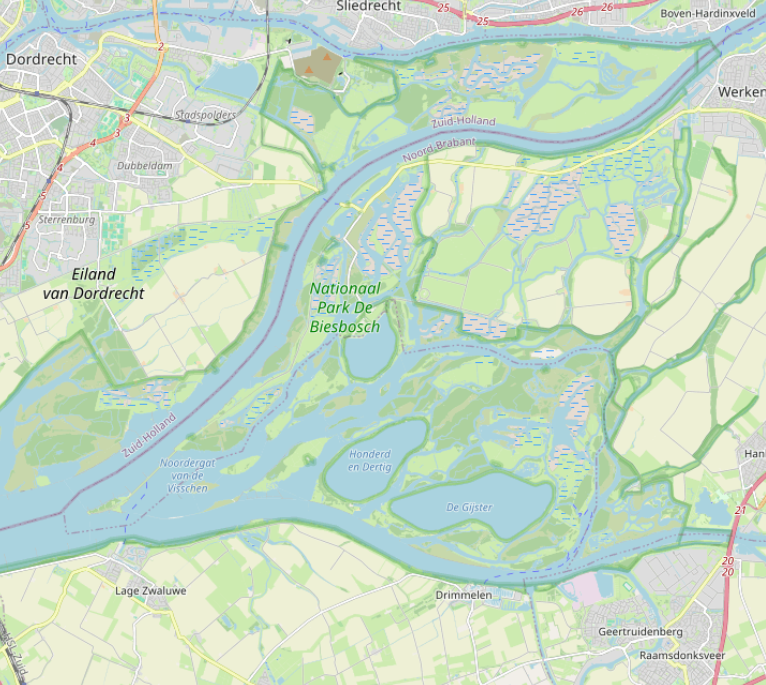
\includegraphics[width=\linewidth]{figs_01/biesbosch_osm.png}
                \caption{The Biesbosch wetlands area in the Netherlands, as represented on OpenStreetMap.}
                \label{fig:first_col_first_fig}
                \vspace{1em} % Space between the figures in the first column
                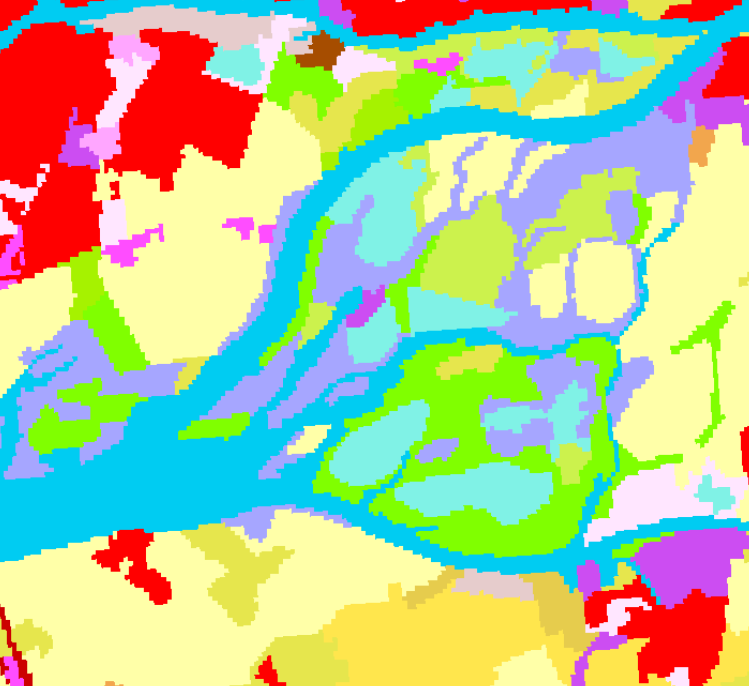
\includegraphics[width=\linewidth]{figs_01/biesbosch_clc.png}
                \caption{The Biesbosch as represented by CORINE Land Cover.}
            \end{minipage}
            \hfill
            % Right column
            \begin{minipage}{0.49\textwidth}
                \centering
                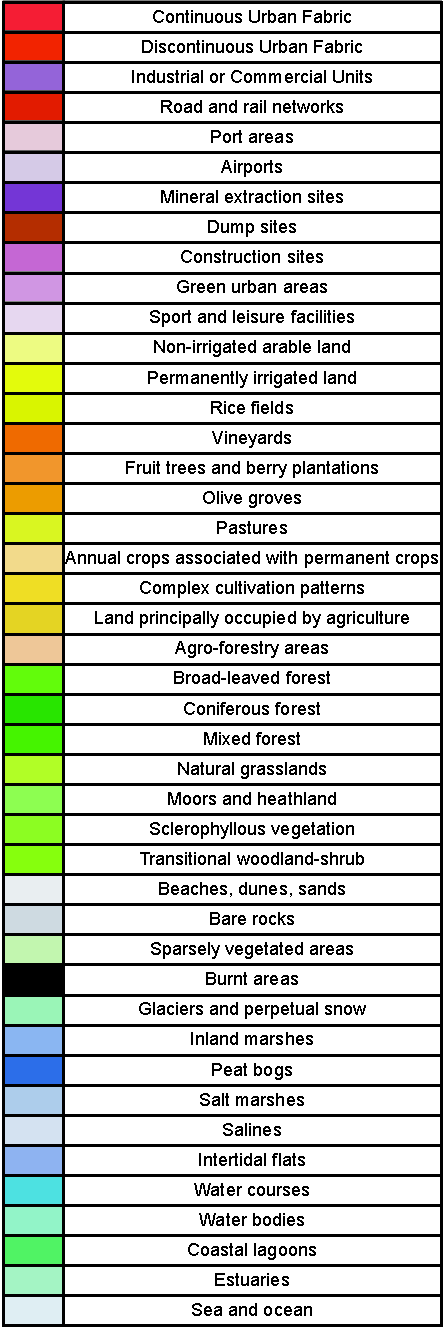
\includegraphics[width=\linewidth,height=2.15\textwidth,keepaspectratio]{figs_01/corine_legend.pdf}
                \caption{The 43-class CORINE Land Cover legend.}
                \label{fig:biesbosch_osm_clc}
            \end{minipage}
            \label{fig:two_column_layout}
        \end{figure}

\subsection{Land cover classification with machine learning and earth observation data}
    
    Automated mapping methods, such as those used by \citet{pflugmacher2019mapping}, \citet{dandrimont2021parcel}, \citet{luo2022developing} and \citet{malinowski2020automated} are called Land Cover Classification. It typically involves showing many good examples of the things you want to detect on a map to a computer program, which then learns how to recognize them by itself when shown new locations. For this, the following three core components are needed:
    
    \begin{itemize}
    \item \textbf{Examples:} Confirmed and annotated observations of different types of land cover, with a known time and place. We often call these observations \textbf{reference data}, \textit{labels}, or \textit{samples}.
    \item \textbf{Earth observation (EO) data:} satellite imagery and other geographic data that cover the area you want to map. Together, these \textbf{covariates} form the \textbf{feature space}. Spatial and temporal metadata allow aspiring mappers to combine several existing, unrelated datasets into one feature space; a rarity in the machine learning domain.
    \item A \textbf{model:} Some kind of decision-making algorithm that learns to recognize which examples often occur at which combination of the covariates. If this goes well, you can use it to \textbf{predict}, or \textit{classify}, which land cover occurs at locations that are covered by the feature space, but where reference data are not available.
    \end{itemize}
    
    It is common to use different sets of reference data: one set to train your model, and one independent set to validate its predictions, namely the land cover maps it has made. It is good if these two datasets were collected separately from each other, because this helps to make sure your model \textbf{generalizes} well: that its predictions are accurate in new situations, not just on the data it was trained on.

    \subsubsection{Training data}

        Training data is a set of labeled observations that are used to teach a machine learning model to recognize similar things in new situations. To make sure your model generalizes well, you have to properly represent the feature space of the area you want to map in your training data \citep{meyer2021predicting}. This does not directly relate to geographical space; large homogeneous areas such as deserts tend to be quite similar in the feature space, while small complex landscapes such as cities with parks, gardens and canals will show great local variation. 

        It is important to have enough training examples \citep{ramezan2021effects,rodriguez-perez2017influence,zhu2016optimizing}, but what is `enough' differs per model \citep{myburgh2014impact} and task \citep{koshute2021recommending}. 
        Models often learn to estimate classes in the same proportions as their training data. If these proportions do not match the real-world situation of the area they need to map, the model may become \textbf{biased}. To minimize this bias and predict the right relative quantities for each class, you need training data that match the desired proportions \citep{he2009learning}.
        
    \subsubsection{Validation data}

        All maps are wrong \citep{monmonier2018how}, and maps produced with machine learning and earth observation data are no exception. Errors can be defined as \textit{quantity disagreement} and \textit{allocation disagreement}: are there enough pixels of every class, and are they in the right place \citep{pontius2006can,pontius2011death}? Ideally, both types of errors should be low. Errors can come from various sources. Some classes might be hard to distinguish in the available feature space, confusing the model \citep{shivakumar2017spectral}. Some classes might be overrepresented in the training data, leading the model to predict it more frequently at the expense of other classes and resulting in low quantity agreement.

        In general, it is essential that any map is validated with a set of observations. Such validation datasets need to be of high quality: their accuracy should surpass the target accuracy of the map and they need to be representative of the classes in the mapped area.
    
        Biased training data can lead to a biased model that overpredicts certain classes. In this case, the proportions of the classes on the map will deviate from the proportions in the real world. It is very difficult to quantify the bias of a model before it is used \citep{stehman2013estimating}, and the current best way of fixing the proportions on a map is to measure the model bias with additional sampling after the mapping is complete \citep{stehman2014estimating}.

        Classification errors become even more troublesome when land cover change is measured by comparing maps from two time periods, as any misclassified pixel will be interpreted as a change \citep{olofsson2013making}. This can be counteracted by careful sampling design \citep{stehman2012impact,olofsson2014good}, although some work has been done to circumvent this and derive area estimates directly from the model predictions \citep{sales2022land,kleinewillinghofer2022unbiased,angelopoulos2023predictionpowered}.
        All in all, it is important to validate annual large-scale maps with up-to date validation data to ensure there is no dataset drift and to properly quantify accuracy and uncertainty \citep{tsendbazar2021towards}.

    \subsubsection{Earth Observation Data}

        Earth observation data refers to measurements taken by sensors at various ranges, from ground measurements \citep{shahi2015novel} to drone \citep{tang2015drone} and airplane \citep{mastelic2020aerial} imagery, to satellite scans \citep{phiri2020sentinel}. The most useful for recurring large-scale mapping are satellite scans, as satellites revisit the same area at a regular pace. This allows them to provide a consistent stream of data, which, in some cases, can continue for decades \citep{xiong2020modis,wulder2022fifty}. The activity of remotely collecting Earth observation data is generally referred to as \textbf{remote sensing}.

        Earth observation data only started becoming openly available after Brazil published its LANDSAT archives as open data in 2008 \citep{nature2008markets}. Afterwards, more and more Earth observation data and land cover information has become openly available. While this rapidly growing landscape of increasingly large datasets on diverging platforms and systems can be hard to navigate \citep{wagemann2021a}, it has fuelled an exponential increase in the amount of mapping initiatives and environmental awareness \citep{wulder2022fifty}, with applications ranging from deforestation \citep{hansen2013high} to soil mapping \citep{hengl2017soilgrids250m}. For further reading on the role of remote sensing in quantifying essential characteristics of the biosphere, cryosphere, and hydrosphere, readers are directed to \citet{radeloff2024need}, which provides an up-to-date review of the state of the art and current needs.
        
        Spatial machine learning is unique in the sense that it allows modelers to easily combine variables if they can somehow acquire a representation of them at the time and place of the ground truth observation, such as with a spatial or spatiotemporal overlay. Combining different data sources can lead to much higher performance, for instance with crop stress detection  \citep{berger2022multi}, urban heat \citep{shahi2015novel}, and land cover classification \citep{zhu2016optimizing, hurskainen2019auxiliary, hosseiny2022urban,xu20183d}. Having data of the same place from different moments \citep{low2013impact} and different spatial resolutions or scales \citep{santos2012multiscale} can also improve mapping accuracy, especially of classes that have very similar spectral profiles and/or cyclical temporal dynamics, such as crops and grassland \citep{esch2014differentiation}.

\subsection*{The current land cover mapping arms race}

   In the past decades, machine learning has been used to make land use and land cover maps at global scales. Due to limitations in the resolution of the available satellite data, such maps were at resolutions of 5~km for GLASS-GLC \citep{liu2020annual}, 300~m for ESA CCI \citep{defourny2012land} or 100~m for Copernicus Global Land Cover \citep{buchhorn2020copernicus}. This made them useful for large scale analysis, but of limited value for local applications and analyses, such as investigating small-scale land use as drivers of deforestation \citep{masolele2024mapping}. However, in the last few years, the increased availability and analysis-readiness of high-resolution from NASA's Landsat and ESA's Sentinel-2 programmes have enabled the creation of global- and continental-scale high-resolution land cover maps by several organizations. Notable examples are ESA's WorldCover \citep{kerchove2021esa} and WorldCereal \citep{tricht2023worldcereal}, Google's DynamicWorld \citep{brown2022dynamic}, ESRI's Land Cover \citep{karra2021global}, and GLAD's Global Land Cover \citep{potapov2022global}.
    These maps often have high resolution and high accuracy, but are usually limited in multiple ways: reproducibility, time coverage, and detail:
    
    \subsubsection{Reproducibility}
        Most of the current big mapping initiatives only share their maps, not the reference data that they used to produce them. This not only makes it difficult or impossible to reproduce, challenge, or improve their work, but also prevents it from being used for new projects \citep{tsendbazar2015assessing}. If they don't share their validation data, independent validations are dependent on open validation datasets \citep{venter2022global}, which might not perfectly match their legend, making a fair comparison more difficult.
    
    \subsubsection{Time coverage} 
        Most of the current generation of maps use 10~m Sentinel-2 data, which only became available in 2016. Mapping initiatives that use Landsat data can go back much further, but are then limited to mapping at 30m resolution. Examples are the Australian land cover time series made by \citep{calderon2021high} and the work of UMD GLAD, which produced annual land cover maps from the year 2000 onwards using Landsat data \citep{hansen2022global}. \citet{garcia2022global} provides an thorough overview of LULC datasets with long-running time series.

    \subsubsection{Detail}
        %Visual interpretation mention specifically!
        Often, these maps depict at most ten land cover categories (see Table~\ref{tab:bigmaps}). Mapping more classes is more difficult because there is more chance of confusion between similar classes. This also applies to the creation of training data: The current most common way to create it is by visual inspection of high resolution aerial or satellite imagery, and this becomes more difficult with more specific classes. Just like for a machine learning model, it is much easier for an annotator to differentiate between a forest and cropland than between different cereal crop types. Classifying more different classes is also more difficult for machine learning models and requires more training data, and of higher quality, which is an expensive and complex task \citep{li2021improving}, especially for large diverse areas (e.g., continents or the whole planet) \citep{tsendbazar2021towards,stanimirova2023global}. 

\begin{figure}[H]
    \centering
    \begin{subfigure}[t]{0.243\textwidth}
        \centering
        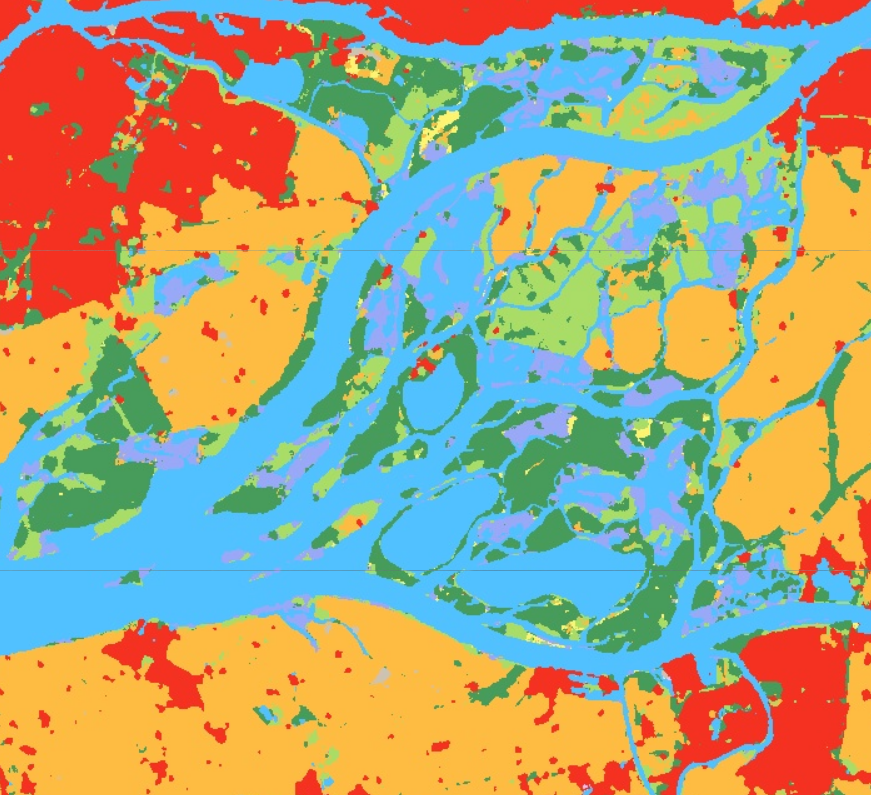
\includegraphics[width=\textwidth,height=\textwidth]{figs_01/a_dynamicworld_clean.png}
    \end{subfigure}
    \hfill % Distribute subfigures evenly in the line
    \begin{subfigure}[t]{0.243\textwidth}
        \centering
        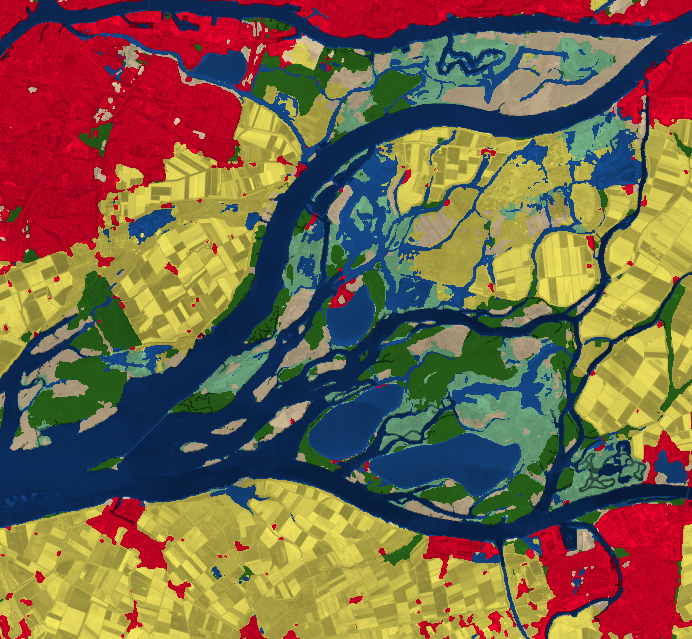
\includegraphics[width=\textwidth,height=\textwidth]{figs_01/a_esri_clean.png}
    \end{subfigure}
    \hfill % Distribute subfigures evenly in the line
    \begin{subfigure}[t]{0.243\textwidth}
        \centering
        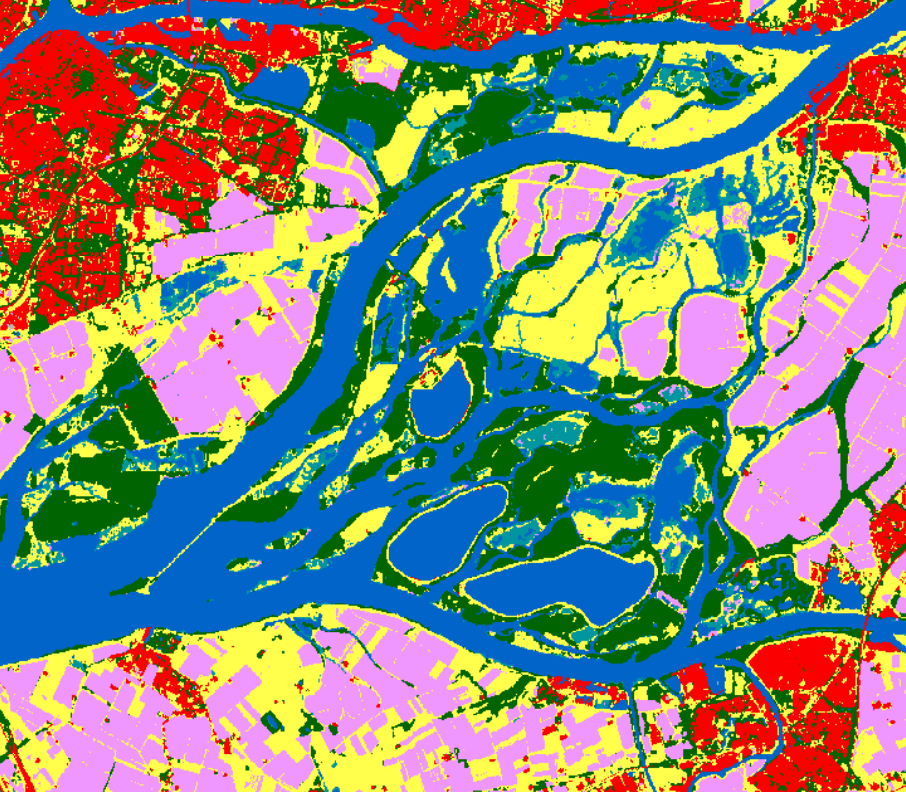
\includegraphics[width=\textwidth,height=\textwidth]{figs_01/a_worldcover_clean.png}
    \end{subfigure}
    \hfill % Distribute subfigures evenly in the line
    \begin{subfigure}[t]{0.243\textwidth}
        \centering
        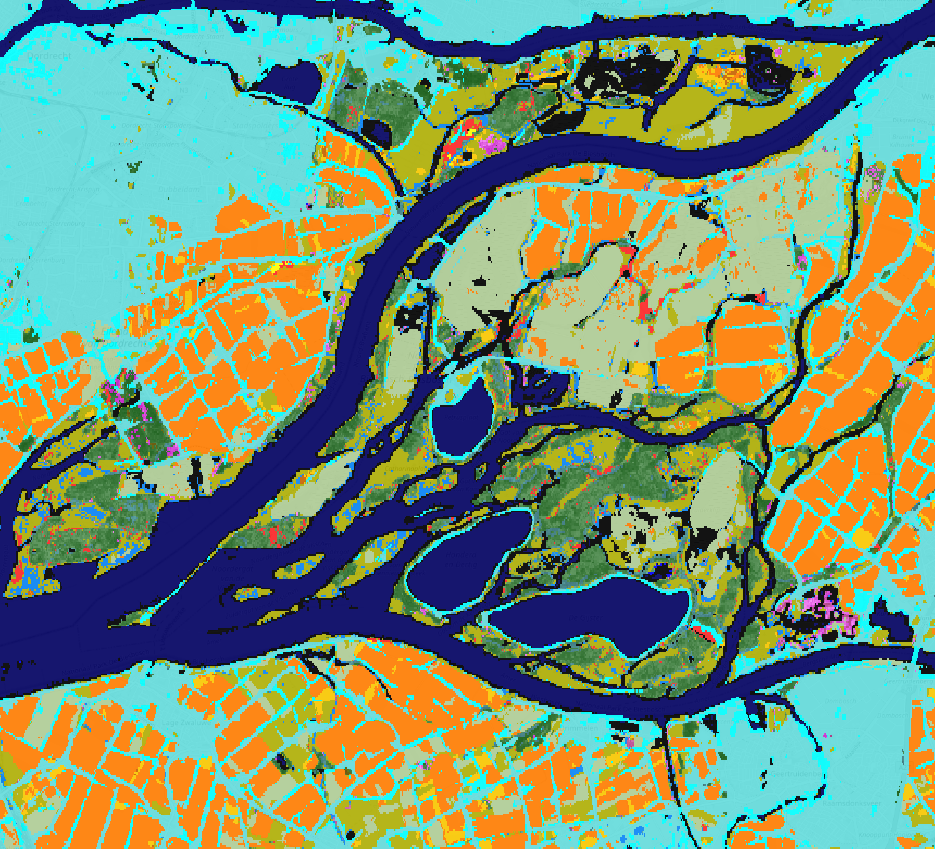
\includegraphics[width=\textwidth,height=\textwidth]{figs_01/a_glad_clean.png}
    \end{subfigure}
    % No \hfill here as we want to force the next subfigure to the next line
    % \vspace{0.1em} % Adds a bit of vertical space between the rows of figures, adjust as needed
    
    \begin{subfigure}[b]{\textwidth}
        \centering
        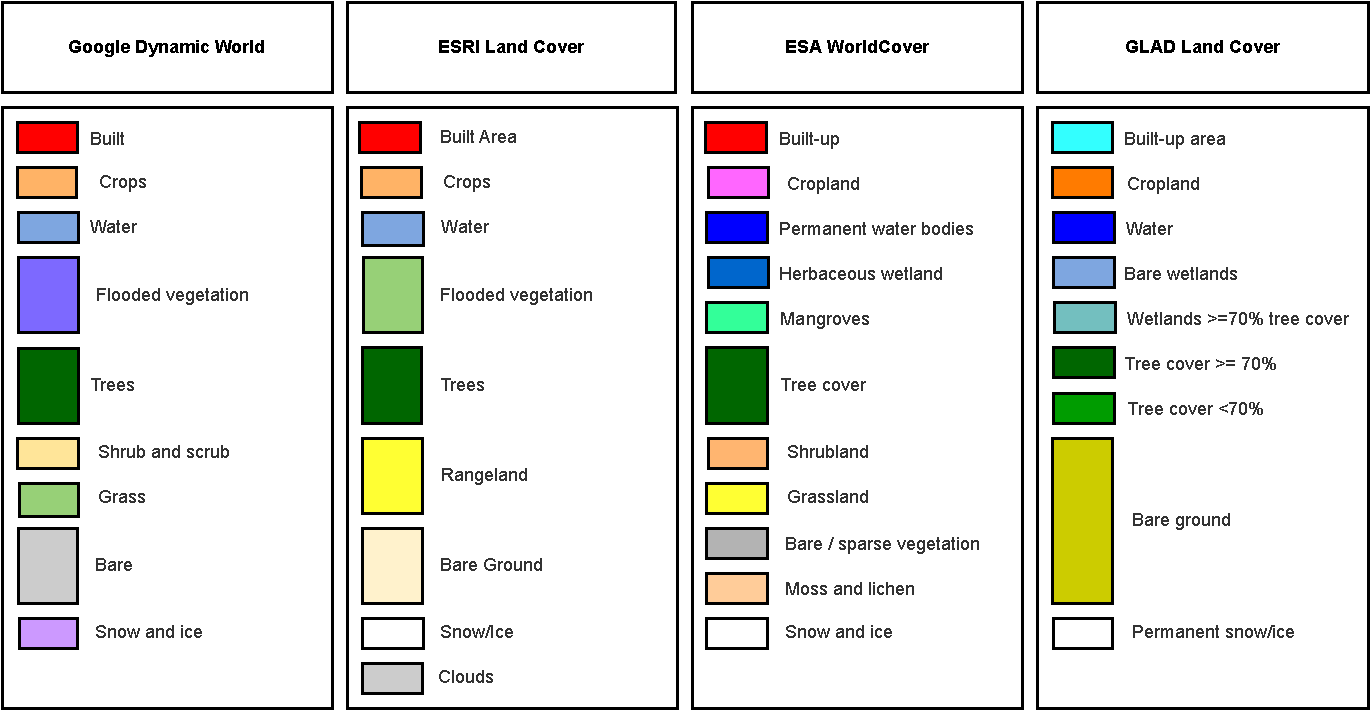
\includegraphics[width=\textwidth]{figs_01/thesis_legends-harmonized.pdf}
    \end{subfigure}
    
    \caption{Comparison of four global mapping projects in the Biesbosch wetlands area in the Netherlands: Google Dynamic World \citep{brown2022dynamic}, ESRI Land Cover \citep{karra2021global}, ESA WorldCover \citep{zanaga2022esa}, and GLAD Land Cover \citep{potapov2022global}. Note that each legend is more specific in some thematic types: GLAD differentiates more strongly based on tree cover, while ESA WorldCover differentiates more between different types of non-forested dry land.}
    \label{fig:bigmaps_biesbosch}
\end{figure}


 
    Although there are exceptions to each of these issues, in general, all of the current mapping initiatives have at least one of these limitations (see Table\@~\ref{tab:bigmaps}). There is value in mapping as far back as possible, something that the previous generation of global maps did do \citep{garcia2022global}. An extreme example is the History database of the Global Environment (HYDE), which contains historic estimated maps at 10~km resolution of main land use categories going back more than 10 thousand years. (Klein Goldewijk et al. 2017). HYDE is also quite detailed, and includes irrigated areas, rice, intensive pasture, extensive rangelands and similar classes. This makes it useful despite its low spatial resolution. Regardless, there is a need for modern maps that do not sacrifice detail to maintain useful spatial resolution and accuracy, and which are made transparently and reproducibly, so that they can be challenged, improved, and trusted.

    \begin{table}[h]
    \centering
    % \resizebox{\textwidth}{!}{%
    % \begin{tabularx}{\textwidth}{|X|X|X|X|X|X|X|}
    \begin{tabularx}{\textwidth}{>{\hsize=1.5\hsize}X|>{\hsize=.7\hsize}X|>{\hsize=.9\hsize}X|>{\hsize=.9\hsize}X|>{\hsize=.7\hsize}X|>{\hsize=.9\hsize}X>{\hsize=.9\hsize}X}
    \toprule
    \textbf{Mapping \makecell{Product}}                                                & \textbf{Classes}  & \textbf{Training Data}                & \textbf{Validation Data}              & \textbf{Spatial Res.} & \textbf{Time Res.}  \\ \hline
    ESA WorldCover \citep{zanaga2022esa}                                    & 11                & No                                    & No                                    & 10~m                      & 2020, 2021            \\ \hline
    ESA WorldCereal \citep{tricht2023worldcereal}                           & 10                & Yes \citep{worldcereal_rdm}           & Yes \citep{lesiv2023global}           & 10~m                      & 2021                  \\ \hline
    Google DynamicWorld \citep{brown2022dynamic}                            & 9                 & Yes \citep{tait2021dwtd}              & No                                    & 10~m                      & 2016+, monthly        \\ \hline 
    ESRI Land Cover \citep{karra2021global}                                 & 9                 & No                                    & No                                    & 10~m                      & 2017--2021, annual    \\ \hline
    \makecell[l]{GLAD Global} \makecell[l]{Land Cover and} \makecell[l]{Land Use} \makecell[l]{Change \citep{potapov2022global}}    & 7                 & No                                    & No                                    & 30~m                      & 2000--2020, annual    \\ \hline 
    GLC\_FC30 \citep{zhang2020glcfcs30}                                     & 30                & No                                    & Yes \citep{liangyun2019dataset}       & 30~m                      & 1982--2021, annual*   \\ \hline
    S2GLC Maps of Europe \citep{malinowski2020automated}                    & 13                & No                                    & Yes \citep{jenerowicz2021validation}  & 10~m                      & 2017                  \\ \hline 
    ELC10 \citep{venter2021continentalscale}                                & 8                 & Yes \citep{dandrimont2020harmonised}  & Yes (cross-validation)                & 10~m                      & 2020                  \\ \hline
    Pan-European land cover \citep{pflugmacher2019mapping}                  & 12                & Yes \citep{dandrimont2020harmonised}  & Yes (cross-validation)                & 30~m                      & One year              \\ \hline 
    Australian Land Cover \citep{calderon2021high}                          & 6                 & No                                    & No                                    & 30~m                      & 1985-2015             \\ \bottomrule
    \end{tabularx}
    % }%
    \caption{Summary of Mapping Products and Data Availability}
    \label{tab:bigmaps}
    \end{table}

    
% Several initiatives aim at integrating multiple land cover products \citep{herold2016toward}(Herold et al. 2016) and/or running land cover classification by fusing multisource EO data \citep{song2017improving,liu2021finer}.
% 
% However, the fact that there is now significant interest in getting the most current, most accurate, and most detailed (spatial resolution) products showing the dynamics of land cover and land use is excellent news! Fair competition should be embraced or as the famous Chinese poem says \emph{``Let a hundred flowers bloom; let a hundred schools of thought contend.''}

\section{Research Gaps}

    There is a reproducibility crisis in science, and environmental monitoring is no exception \citep{treves2022best, powers2018open}. How can decision-makers trust datasets whose creation does not only involve complex workflows, but can not be reproduced or improved? It turns out that they often don't, and keep relying on older methods that might be slow and expensive, but reproducible and reliable. The current boom in for-profit remote sensing has allowed for excellent analysis using high-resolution data ---e.g., drivers of deforestation in Africa \citep{masolele2024mapping} using 3~m resolution Planet data--- but limitations on sharing this data, and the profit and marketing motivations of corporations make sharing, trusting, and using their maps difficult.

    There are no reproducible large-scale maps with more than 13 classes, not even for Europe, for which an unprecedented wealth of land cover information is publicly available \citep{dandrimont2020harmonised}. \citet{pflugmacher2019mapping} demonstrated that the LUCAS points can be used to train and validate land cover models, but the LUCAS legend is a hierarchical system with over 70 land cover and land use classes. To retain its use as a validation set, training data should be extracted from other human-annotated datasets such as CORINE, EuroCrops \citep{schneider2023eurocrops} and OpenStreetMap \citep{schultz2017open}.  In order to use data with the large minimal mapping unit of CORINE or the potential errors in volunteered geographical information \citep{neis2014recent}, filtering techniques are required to remove spurious training samples.

    Furthermore, while some long-term annual mapping projects exist, they either have a low spatial resolution like ESA CCI \citep{harper202229}, cover only a select set of classes \citep{potapov2022global}, or did not publish their training data \citep{zhang2020glcfcs30}. 

    Lastly, to evaluate the impacts of human activities on the environment and to both enable and justify localized interventions, it is essential that trends from area estimates and periodic maps are linked \citep{olofsson2014good,szantoi2020addressing,winkler2021global}. This requires a mapping framework that minimizes both quantity and allocation error \citep{pontius2011death}. While many mapping initiatives report class proportions \citep{pflugmacher2019mapping} or try to approximate correct area estimation with direct remote sensing measures \citep{kleinewillinghofer2022unbiased}, only a few explicitly investigate methods to force maps to match area estimates \citep{strahler1980use,horvath2021comparison}.
    

\section{Objectives}
\label{sec:research_objectives}
The overall objective of this PhD thesis is to take advantage of the availability of various open European land use / land cover datasets and statistics, and to combine these with Earth observation data and machine learning to make accurate, detailed maps that are compatible with the needs of European policy makers and researchers. More specifically, this thesis aims to answer the following research questions:

\begin{enumerate}
\item %The Value of Aggregating and Combining Time-Series and Static EO Data for Land Cover Classification: 
What are the benefits and challenges of combining multiple large time-series and static EO datasets into analysis-ready data for the purpose of land cover classification?
\item % The Value of a Spatiotemporal Approach for Land Cover Classification: 
To what extent does training data from multiple times and places improve the accuracy and generalization of land cover classification?
\item % The Effect of Legend Design and Size: 
How does the number and type of classes in a legend affect the accuracy of land cover classification?
\item % Ensuring Land Cover Maps Match Area Estimates Without Sacrificing Accuracy: 
What is the effect of enforcing design-based class proportions on map accuracy?
\end{enumerate}

\section{Thesis Outline}

The research questions posed in the previous section are answered through four research papers, which are presented as chapters in this thesis. Fig.\@~\ref{fig:01_rqs_chapters} provides a graphical overview of how each chapter relates to each research question framework. The first two chapters focus on combining earth observation and land cover data from multiple sources to train models that can generalize well to unknown years. Chapter\@~\ref{cha:chapter4} applies a novel algorithm that uses a-priori class proportions from area estimates to optimize the accuracy and quantity of predictions by such models.

\begin{figure}[H]
    \centering
    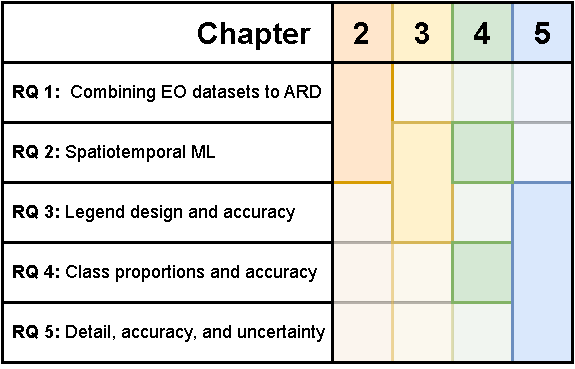
\includegraphics[width=.55\textwidth]{figs_01/fig_rqs_chapters.pdf}
    \caption{Overview of which chapters discuss which research questions.}
    \label{fig:01_rqs_chapters}
\end{figure}

\textbf{Chapter 2} focuses on the benefits and challenges of harmonizing and combining large-scale spatiotemporal datasets for land cover mapping, most of which were used in the following chapters. The chapter details the work that went into creating, harmonizing, and imputing multiple Earth observation datasets (Landsat, Sentinel-2, and a new 30m resolution DTM) covering Europe. It introduces and describes the imputation algorithm TMWM that was used to impute the Landsat data, and validates its accuracy in a spatiotemporally explicit way. It then explores how combining the different datasets improves the accuracy of land cover classification models. Lastly, it shows that models trained on samples from a longer time range can generalize better to years that they have not been trained on.

\textbf{Chapter 3} focuses on the production of annual land use / land cover maps of Europe for 2000-2020. It details the steps taken to harmonize and clean the training data from multiple openly available sources (CORINE, LUCAS) into a legend with 43 classes. A thorough accuracy assessment using cross-validation and an independent set of S2GLC validation points describes how well the model generalizes across space and time, and quantifies the trade-off imposed by having a legend with high thematic resolution. Results show that the maps have similar accuracy as other current continental-scale maps at low thematic resolution, and that a more detailed legend introduces more errors.

\textbf{Chapter 4} introduces IMP, an algorithm that uses land cover area estimates to iteratively classify land cover from existing probabilities, producing maps whose class proportions match the input estimates. It details the algorithm and showcases its use by mapping five European countries in five years. The accuracy of the maps is compared with maps created using highest likelihood classification. Results show that the proportional maps do not only have more accurate class proportions, but equal or better accuracy than highest likelihood maps. We also compare the accuracy and proportions of maps based on probabilities predicted by models trained on data representative of the area of interest, and probabilities predicted by a general model trained on large parts of Europe. Results show that maps based on general model predictions reach more accurate class proportions, while maps based on local model predictions are slightly more accurate. Finally, it presents an unintentional finding that the iterations at which the algorithm classifies certain pixels is related to the accuracy of those pixels, suggesting that it can be used to generate pixel-level accuracy estimates. % Introduction 
	\chapter[Analysis-Ready Data cube]{An Analysis-Ready Data cube for European-scale land cover mapping}
\label{cha:chapter2}
\vspace*{\fill}
This chapter is based on:
\\
\\
% Full citation of the published (or submitted/in review) article
% This refers to the article key in the refs.bib file.
\fullcite{witjes2023ecodatacube}
\newpage

\section*{Abstract}
The paper describes the production steps and accuracy assessment of an analysis-ready, open-access European data cube consisting of 2000--2020+ Landsat data, 2017--2021+ Sentinel-2 data and a 30~m resolution Digital Terrain Model (DTM). The main purpose of the data cube is to make annual continental-scale spatiotemporal machine learning tasks accessible to a wider user base by providing a spatially and temporally consistent multidimensional feature space. This has required systematic spatiotemporal harmonization, efficient compression, and imputation of missing values. Sentinel-2 and Landsat reflectance values were aggregated into four quarterly averages approximating the four seasons common in Europe (winter, spring, summer and autumn), as well as the 25th and 75th percentile, in order to retain intra-seasonal variance. Remaining missing data in the Landsat time-series was imputed with a temporal moving window median (TMWM) approach.  An accuracy assessment shows TMWM performs relatively better in Southern Europe and lower in mountainous regions such as the Scandinavian Mountains, the Alps, and the Pyrenees. We quantify the usability of the different component data sets for spatiotemporal machine learning tasks with a series of land cover classification experiments, which show that models utilizing the full feature space (30~m DTM, 30~m Landsat, 30~m and 10~m Sentinel-2) yield the highest land cover classification accuracy, with different data sets improving the results for different land cover classes. The data sets presented in the paper are part of the EcoDataCube platform, which also hosts open vegetation, soil, and land use / land cover (LULC) maps created. All data sets are available under CC-BY license as Cloud-Optimized GeoTIFFs (ca.\@ 12~TB in size) through SpatioTemporal Asset Catalog (STAC) and the EcoDataCube data portal.

\newpage

\section{Introduction}

Over recent decades, the world has experienced rapid growth in Earth Observation (EO) technology. This has brought many benefits to various applied fields, however, it also brings new challenges to aspiring users: massive data volumes produced by EO sensors and \emph{in-situ} monitoring networks require new specialized expertise and extensive computing capacity. \citet{wagemann2021a} lists the following five key challenges to finding, accessing, and combining big environmental data: (1) limited processing capacity on user side, (2) growing data volumes, (3) non-standardized data formats and dissemination workflows, (4) too many data portals, and (5) difficult data discovery. Environmental data needs to be as accessible and useful as possible, while all its limitations, caveats and uncertainties need to be clearly documented to minimize the risk of error propagation. In addition, decision-makers require easy access to open environmental data and critical assessment tools in order to dynamically synthesize the information needed to address many critical environmental and economic challenges \citep{giuliani2017building}. The European Green Deal specifically \citep{sikora2021european} requires a diversity of environmental information to reach its ambitious project goals, especially those focused on reaching climate neutrality, preservation of natural capital, modernization and simplification of the Common Agricultural Policy (CAP), and connecting farms to forks, all whilst enabling the socio-economic transformation of rural and agricultural areas. 

To enhance environmental data use for decision-making, several groups in different areas around the world have been putting effort in building \emph{EO data cubes}: spatially aligned time-series of calibrated multi-dimensional observations \citep{giuliani2017building}; also see \citet{lu2018multidimensional, liu2021production, mirmazloumi2022elulc}. Some prominent examples of EO data cubes include the Earth System Data Cube \citep{mahecha2020earth}, Digital Earth Australia \citep{lucas2019land}, Digital Earth Africa \citep{fang2021analysis}, and the Swiss Data Cube \citep{chatenoux2021swiss}. Infrastructures such as the openEO Platform (\url{https://openeo.cloud/}), and Google Earth Engine (\url{https://developers.google.com/earth-engine}) can also be considered EO data cubes \citep{giuliani2020data} due to the ease with which users can combine the various data sets hosted on these platforms.

Two important EO data sources in this context are Sentinel-2 and Landsat. 
Sentinel-2 has provided global coverage every five days since the launch of its second satellite (Sentinel-2B) in 2017, available freely from multiple sources such as \url{https://scihub.copernicus.eu} and \url{https://earthexplorer.usgs.gov/}. In recent years it has served as input data for various global and continental land cover mapping initiatives, such as ESA's Worldcover \citep{kerchove2021esa}, Google's DynamicWorld \citep{brown2022dynamic}, and Sentinel-2 Global Land Cover (S2GLC) \citep{malinowski2020automated}. The spatial resolution of Sentinel-2 sensors varies; the red, green, blue, and near-infrared (NIR) bands are available at 10~m resolution, while the two shortwave infrared (SWIR) bands are only available at 20~m.

The Landsat program is the world's longest continuously running EO mission \citep{wulder2022fifty}. It is \emph{de facto} the only option for assessing long-term dynamics as it provides an uninterrupted supply of satellite imagery since 1972. The entire archive was made available to the public in 2008, leading to widespread use, including refinement into data sets closer to analysis-ready status. The University of Maryland (UMD) Global Land Analysis and Discovery (GLAD) laboratory's Landsat ARD product is another representative example of long-term EO data due to its free availability, global coverage, and its inclusion and harmonization of a succession of Landsat satellite sources \citep{potapov2020landsat}. The original data is available in 23{\texttimes} 16--day scenes per year in scaled long format \citep{potapov2020landsat}. While this high temporal resolution and numerical precision provide a large amount of information for subsequent modeling and has been successfully utilized as such by teams with access to large computational resources \citep{hansen2022global}, the added benefit for Land Use Land Cover (LULC) classification compared with a compressed, more accessible form, has not yet been quantified. Furthermore, although the data set is nominally analysis-ready, we encountered the following limitations of using this data set for actual Machine Learning for the purpose of vegetation / land cover mapping:

\begin{itemize}[noitemsep]
\item The data volume of GLAD's original archive (23 4-byte values, or 92 bytes per band per pixel per year) may exclude users without advanced computational capacity from performing country- or continental-scale analysis;
\item While multiple Sentinel-2 data sets are now available from 2015 (Copernicus Sentinel program), a harmonized, cloud-optimized product that is freely accessible regardless of institutional membership and computational resources could greatly increase global usage, especially among marginalized users.
\item While the aggregation to 23 16-day reflectance values increases coverage, gaps remain in the archive due to e.g. snow cover.
\end{itemize}

To maximize the usability of the produced data sets and facilitate future work in annual mapping, we have built a data cube and a data portal available on \url{https://EcoDataCube.eu}. It integrates various layers into a single seamless expandable and open access system. In this paper, we describe the key processing steps used to produce data cubes. We first explain the process of obtaining, gap-filling, artifact removal, and harmonization of EO images: gap-filled Landsat time series from 2000--2020, two Sentinel-2 time-series from 2018--2021 at varying temporal and spatial resolutions, and an optimized Digital Terrain Model created with an ensemble machine learning approach. Finally, we provide examples of EcoDataCube usage and demonstrate case studies for which this data cube provided the main feature space, such as annual LULC maps \citep{witjes2022spatiotemporal} and potential and realized tree distribution \citep{bonannella2022forest}.

\section*{Methods and Data}
In this work we detail the processing and validation workflows of the following four data sets:
\begin{enumerate}
\item Quarterly spatiotemporal Landsat aggregates (median, 75th, and 25th percentile) of blue, green, red, NIR, SWIR1, SWIR2, and thermal bands at 30~m resolution between 2000 and 2020.
\item Two spatiotemporal aggregates (median, 75th and 25th percentiles) of Sentinel-2 between 2018 and 2021:
\begin{enumerate}
\item Annual blue, green, red, and NIR at 10~m resolution;
\item Quarterly blue, green, red, NIR, SWIR1 and SWIR2 bands at 30~m resolution;
\end{enumerate}
\item An optimized Digital Terrain Model (DTM) for Europe, created with an ensemble machine learning data fusion approach.
\end{enumerate}

In order to quantify the extent to which these data sets complement each other as a single feature space for annual mapping with machine learning, we include a series of land cover classification experiments where we compare model performance when trained on different combinations of EcoDataCube layers. Fig.\@~\ref{fig:1_methods_workflow} provides an overview of the general workflow and the resulting output and findings. These data sets all cover the exact same area, which is defined by all member and partner states of the European Environment Agency (EEA) in 2019, with the exception of Turkey (See Fig.\@~\ref{fig:2_study_area_satellite_input}-A).

%f
\begin{figure}[!hbt]
\centering
% \hspace*{-2.9cm}
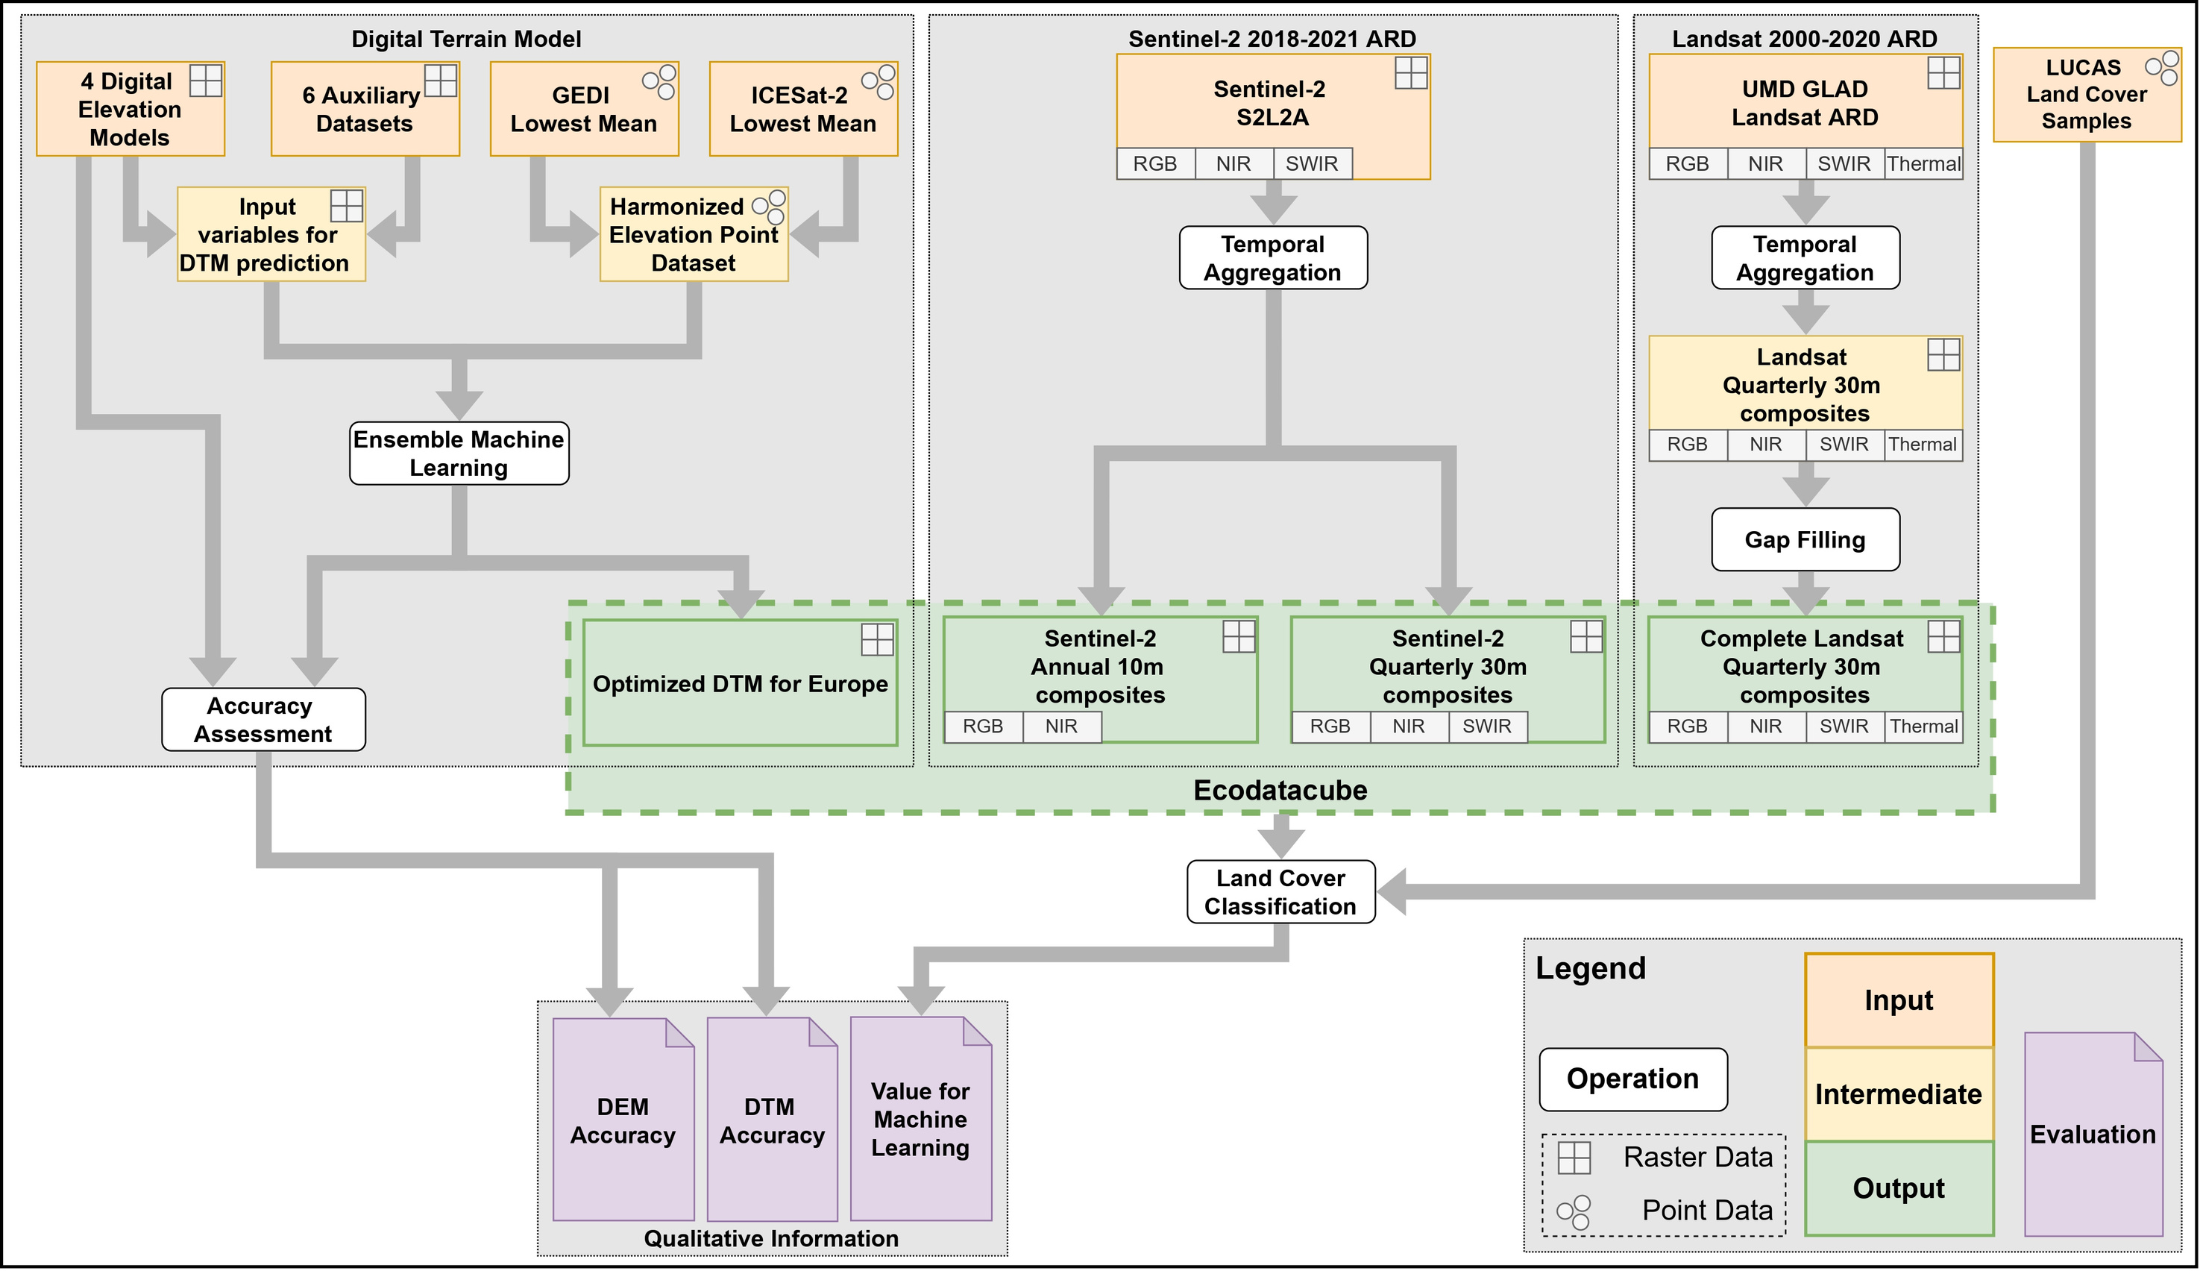
\includegraphics[width=1\textwidth]{figs_02/fig_1_main_workflow.png}
\caption{Overview of the general workflow with input, intermediate, and output data sets, as well as operations and evaluations of data set quality.}
\label{fig:1_methods_workflow}
\end{figure}


\begin{figure}
    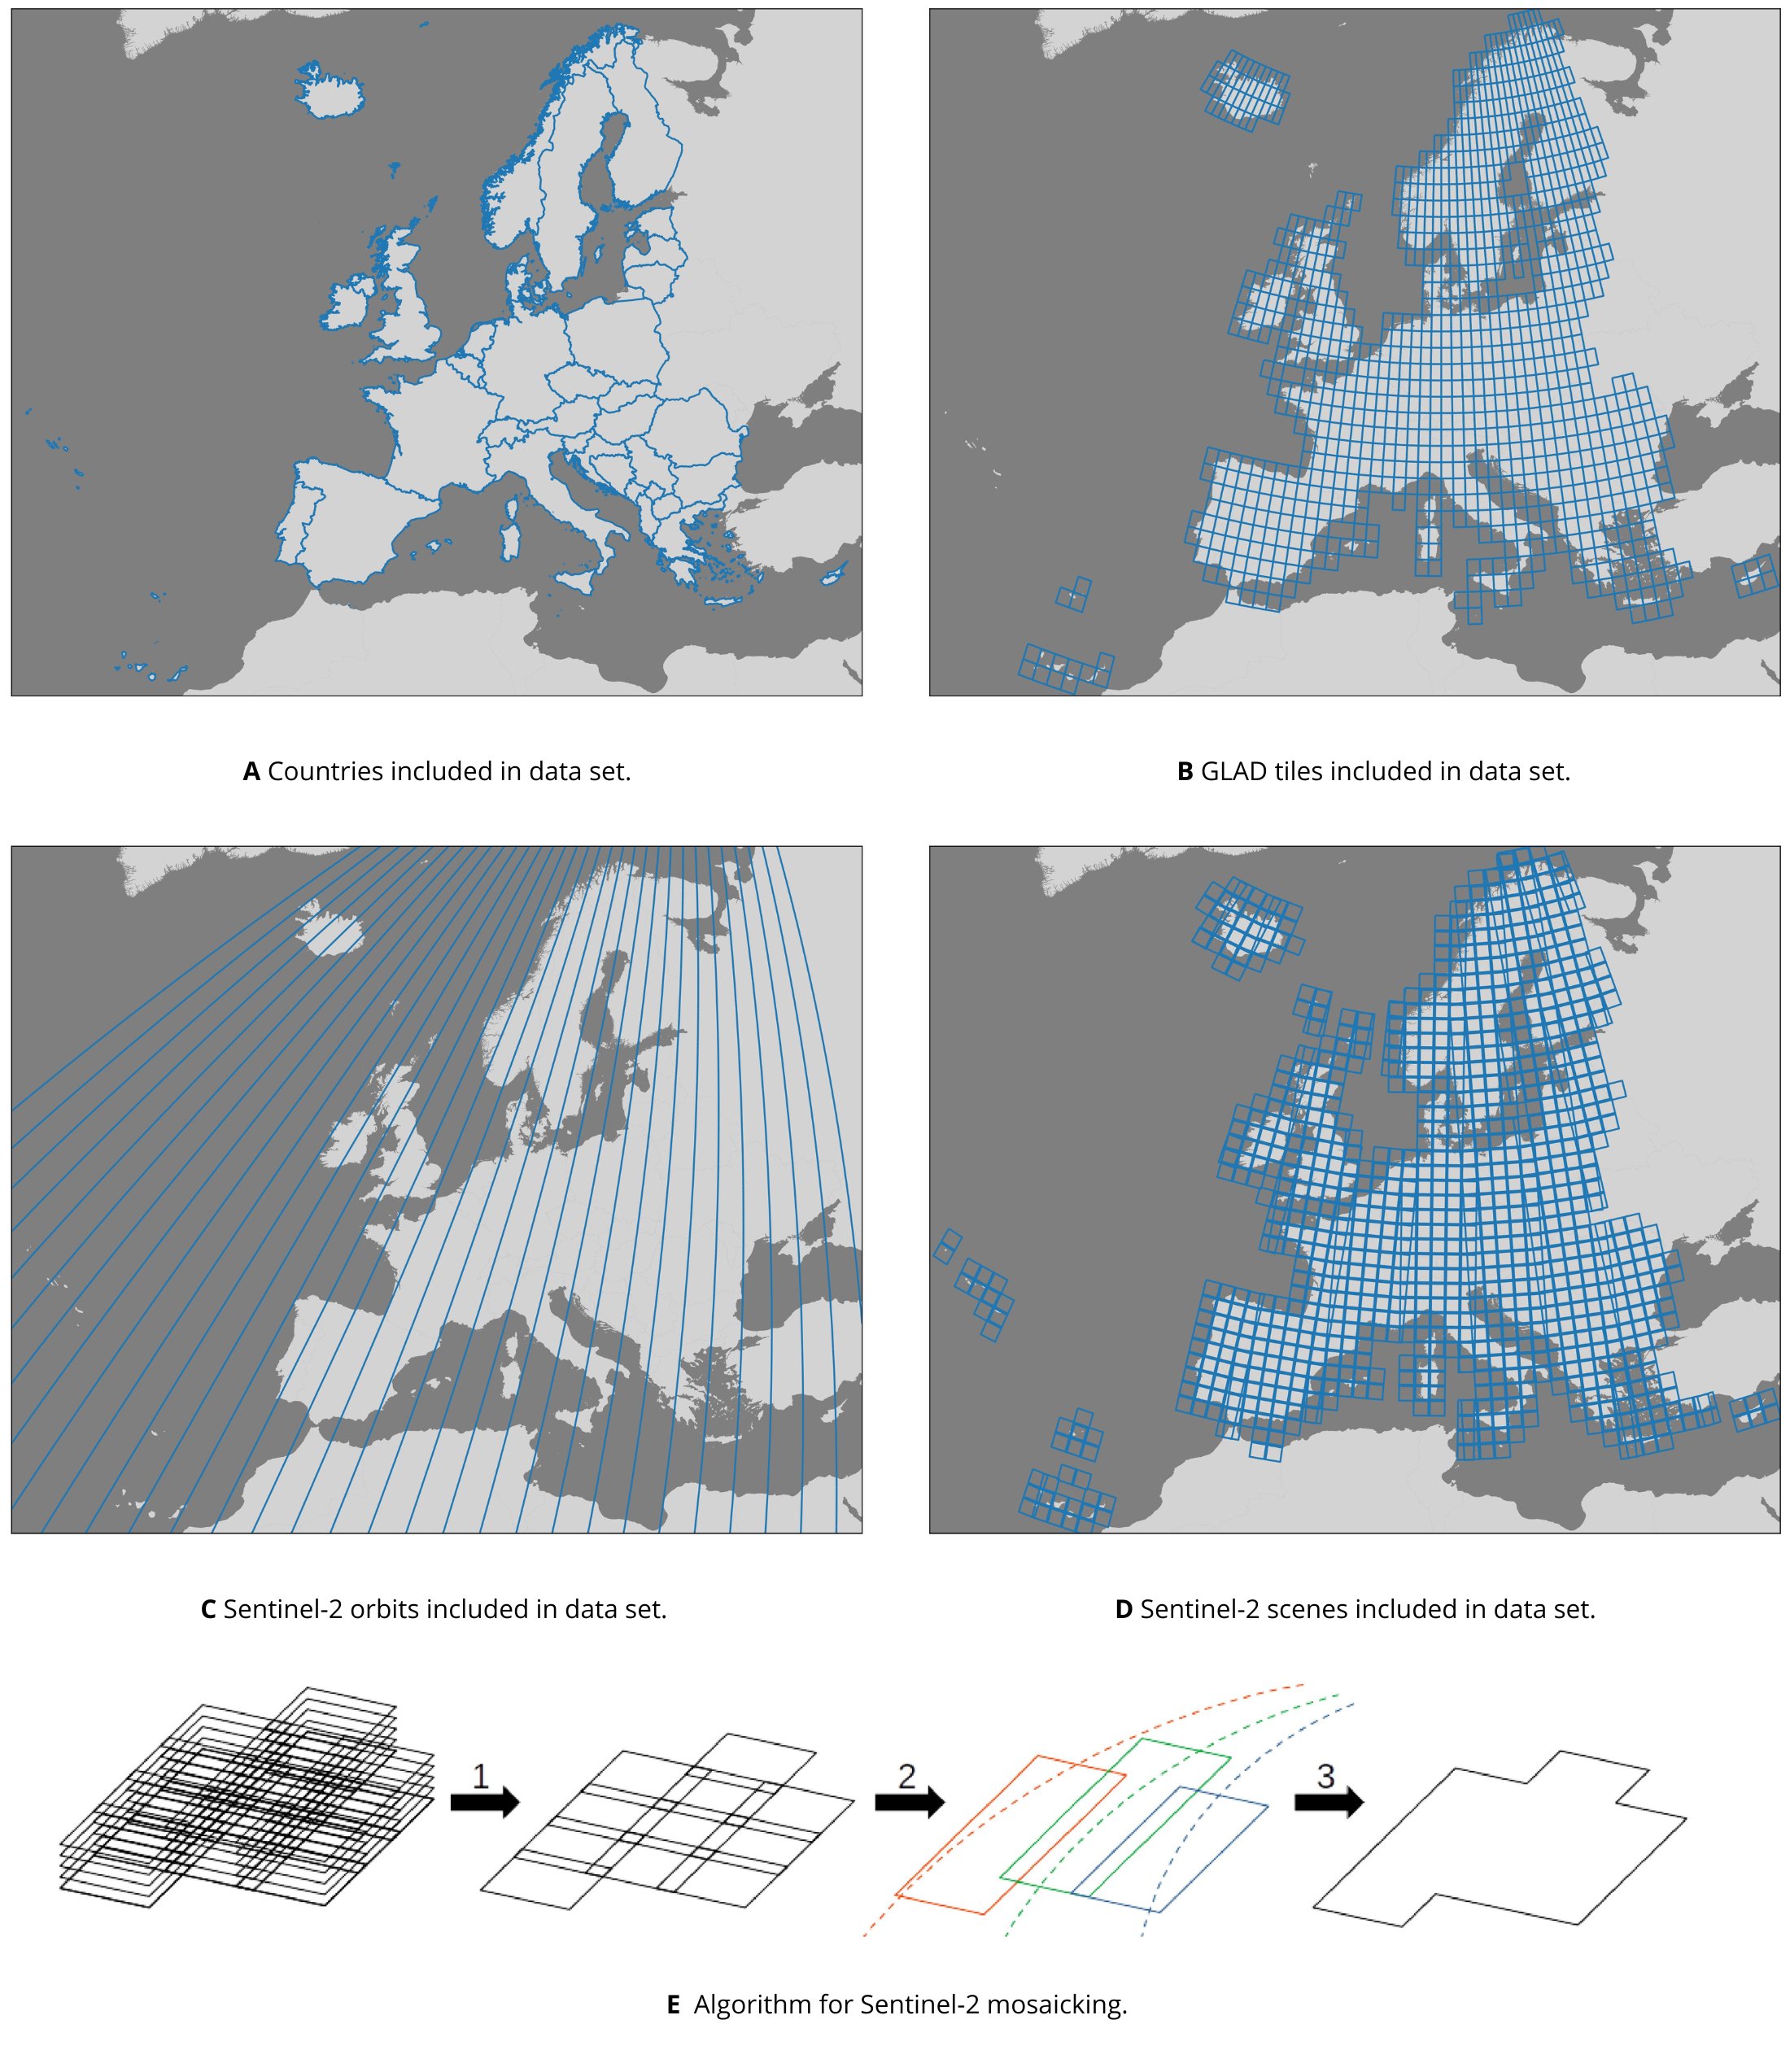
\includegraphics[width=\linewidth]{figs_02/fig_2_study_area_satellite_input.png}
    \caption{Overview of A: the area of interest, B: GLAD Landsat ARD tiles , C-D: Sentinel-2 orbits and scenes used as input sources, and E: the mosaicking algorithm that 1) computes quarterly composites, 2) mosaics the quarterly composites along orbital tracks, and 3) stitches the orbital track mosaics into a single data set.} 
    \label{fig:2_study_area_satellite_input}
\end{figure}



\subsection*{Landsat}
For this work, we used the Landsat Analysis-Ready Data (ARD) product developed by the UMD's GLAD lab, a globally consistent analysis-ready data set for multi-decadal LULC monitoring \citep{potapov2020landsat}. It consists of 16-day time-series composites (23 per year, see Table~\ref{tab:quartiles}) from Landsat 5, 7 and 8 which have been calibrated using MODIS surface reflectance. 

Table~\ref{tab:landsat_sources} shows the bands, their spectral range in the different Landsat sources, and their spatial resolution. These time-series are freely available in 1--degree tiles (see Fig.\@~\ref{fig:2_study_area_satellite_input}-B) and has been screened to flag pixels that likely contain clouds and their shadows in a quality assessment (QA) layer. While this data set is already a level 3 remote sensing product (i.e.\@ temporal composites of gridded data), we aim to make it both more analysis-ready and easier to use by compressing it and imputing any missing values in a computationally efficient way that yields values suitable for classification tasks.

\begin{table}[]
\centering
\caption{Overview of the start and end dates of the four temporal composite periods (quartiles) and of which GLAD interval IDs they were composed.}
\label{tab:quartiles}
\begin{tabular}{@{}l|ll|ll@{}}
\hline
            & Date                          &                   & GLAD interval ID      &       \\
Quartile    & Start                         & End               & Start                 & End   \\
\hline
1           & December 2nd of previous year & March 20nd        & 22 of previous year   & 5   \\
2           & March 21st                    & June 24th         & 6                     & 11 \\
3           & June 25th                     & September 12th    & 12                    & 16 \\
4           & September 13th                & December 1st      & 17                    & 21 \\ 
\hline
\end{tabular}
\end{table}

\begin{table}[]
\centering
\caption{Spectral bands used by \citet{potapov2020landsat} to create the GLAD Landsat ARD data set from multiple Landsat sensors.}
\label{tab:landsat_sources}
\begin{tabular}{@{}cccc@{}}
\hline
Sensor & Landsat 5 & Landsat 7 & Landsat 8 \\ 
Time range                  & 2000--2011     & 2000--2021     & 2013--2021     \\
Band                        & \multicolumn{3}{c}{Wavelength (nm)}           \\ 
\hline
Blue                        & 450-–520       & 441--514       & 452–-512       \\
Green                       & 520-–600       & 519–-601       & 533–-590       \\
Red                         & 630-–690       & 631–-692       & 636–-673       \\
NIR          & 760-–900     & 772–-898       & 851-–879       \\
SWIR1                       & 1,550-–1,750   & 1,547–-1,749   & 1,566–-1,651   \\
SWIR2                       & 2,080-–2,350   & 2,064–-2,345   & 2,107-–2,294   \\
Thermal                     & 10,410-–12,500 & 10,310–-12,360 & 10,600–-11,190 \\ \hline
\end{tabular}
\end{table}
    
\subsubsection*{Landsat Temporal Composites}
\label{sec:landsat-temporal-composites}

In order to balance the trade-off between computation time of large areas while retaining as much temporal variability as possible, we aggregated the 23 annual GLAD Landsat ARD values into four annual quarterly period medians based on the astronomical seasons described by \citet{trenberth1983seasons}, which allows the four periods to act as a proxy for the four typical seasons in large parts of Europe: winter, spring, summer, and autumn. This allows us to match the beginning and end of each period with the 16-day intervals used by \citet{potapov2020landsat} (see Table.\@~\ref{tab:quartiles} and Fig.\@\ref{fig:3_methods_satellite_comparison_and_intervals_seasons_quartiles}-B). We also calculated the 25th and 75th percentile of these aggregated values per pixel in order to maintain a measure of variance within each period that might be useful to recognize intra-annual dynamics. This yields 84 layers for each year (4 quarterly periods $\times$ 3 percentiles $\times$ 7 Landsat bands, see Fig.\@~\ref{fig:3_methods_satellite_comparison_and_intervals_seasons_quartiles}-A) with varying amounts of no-data values based on cloud and snow cover.

%f
\begin{figure}[!hbt]
\centering
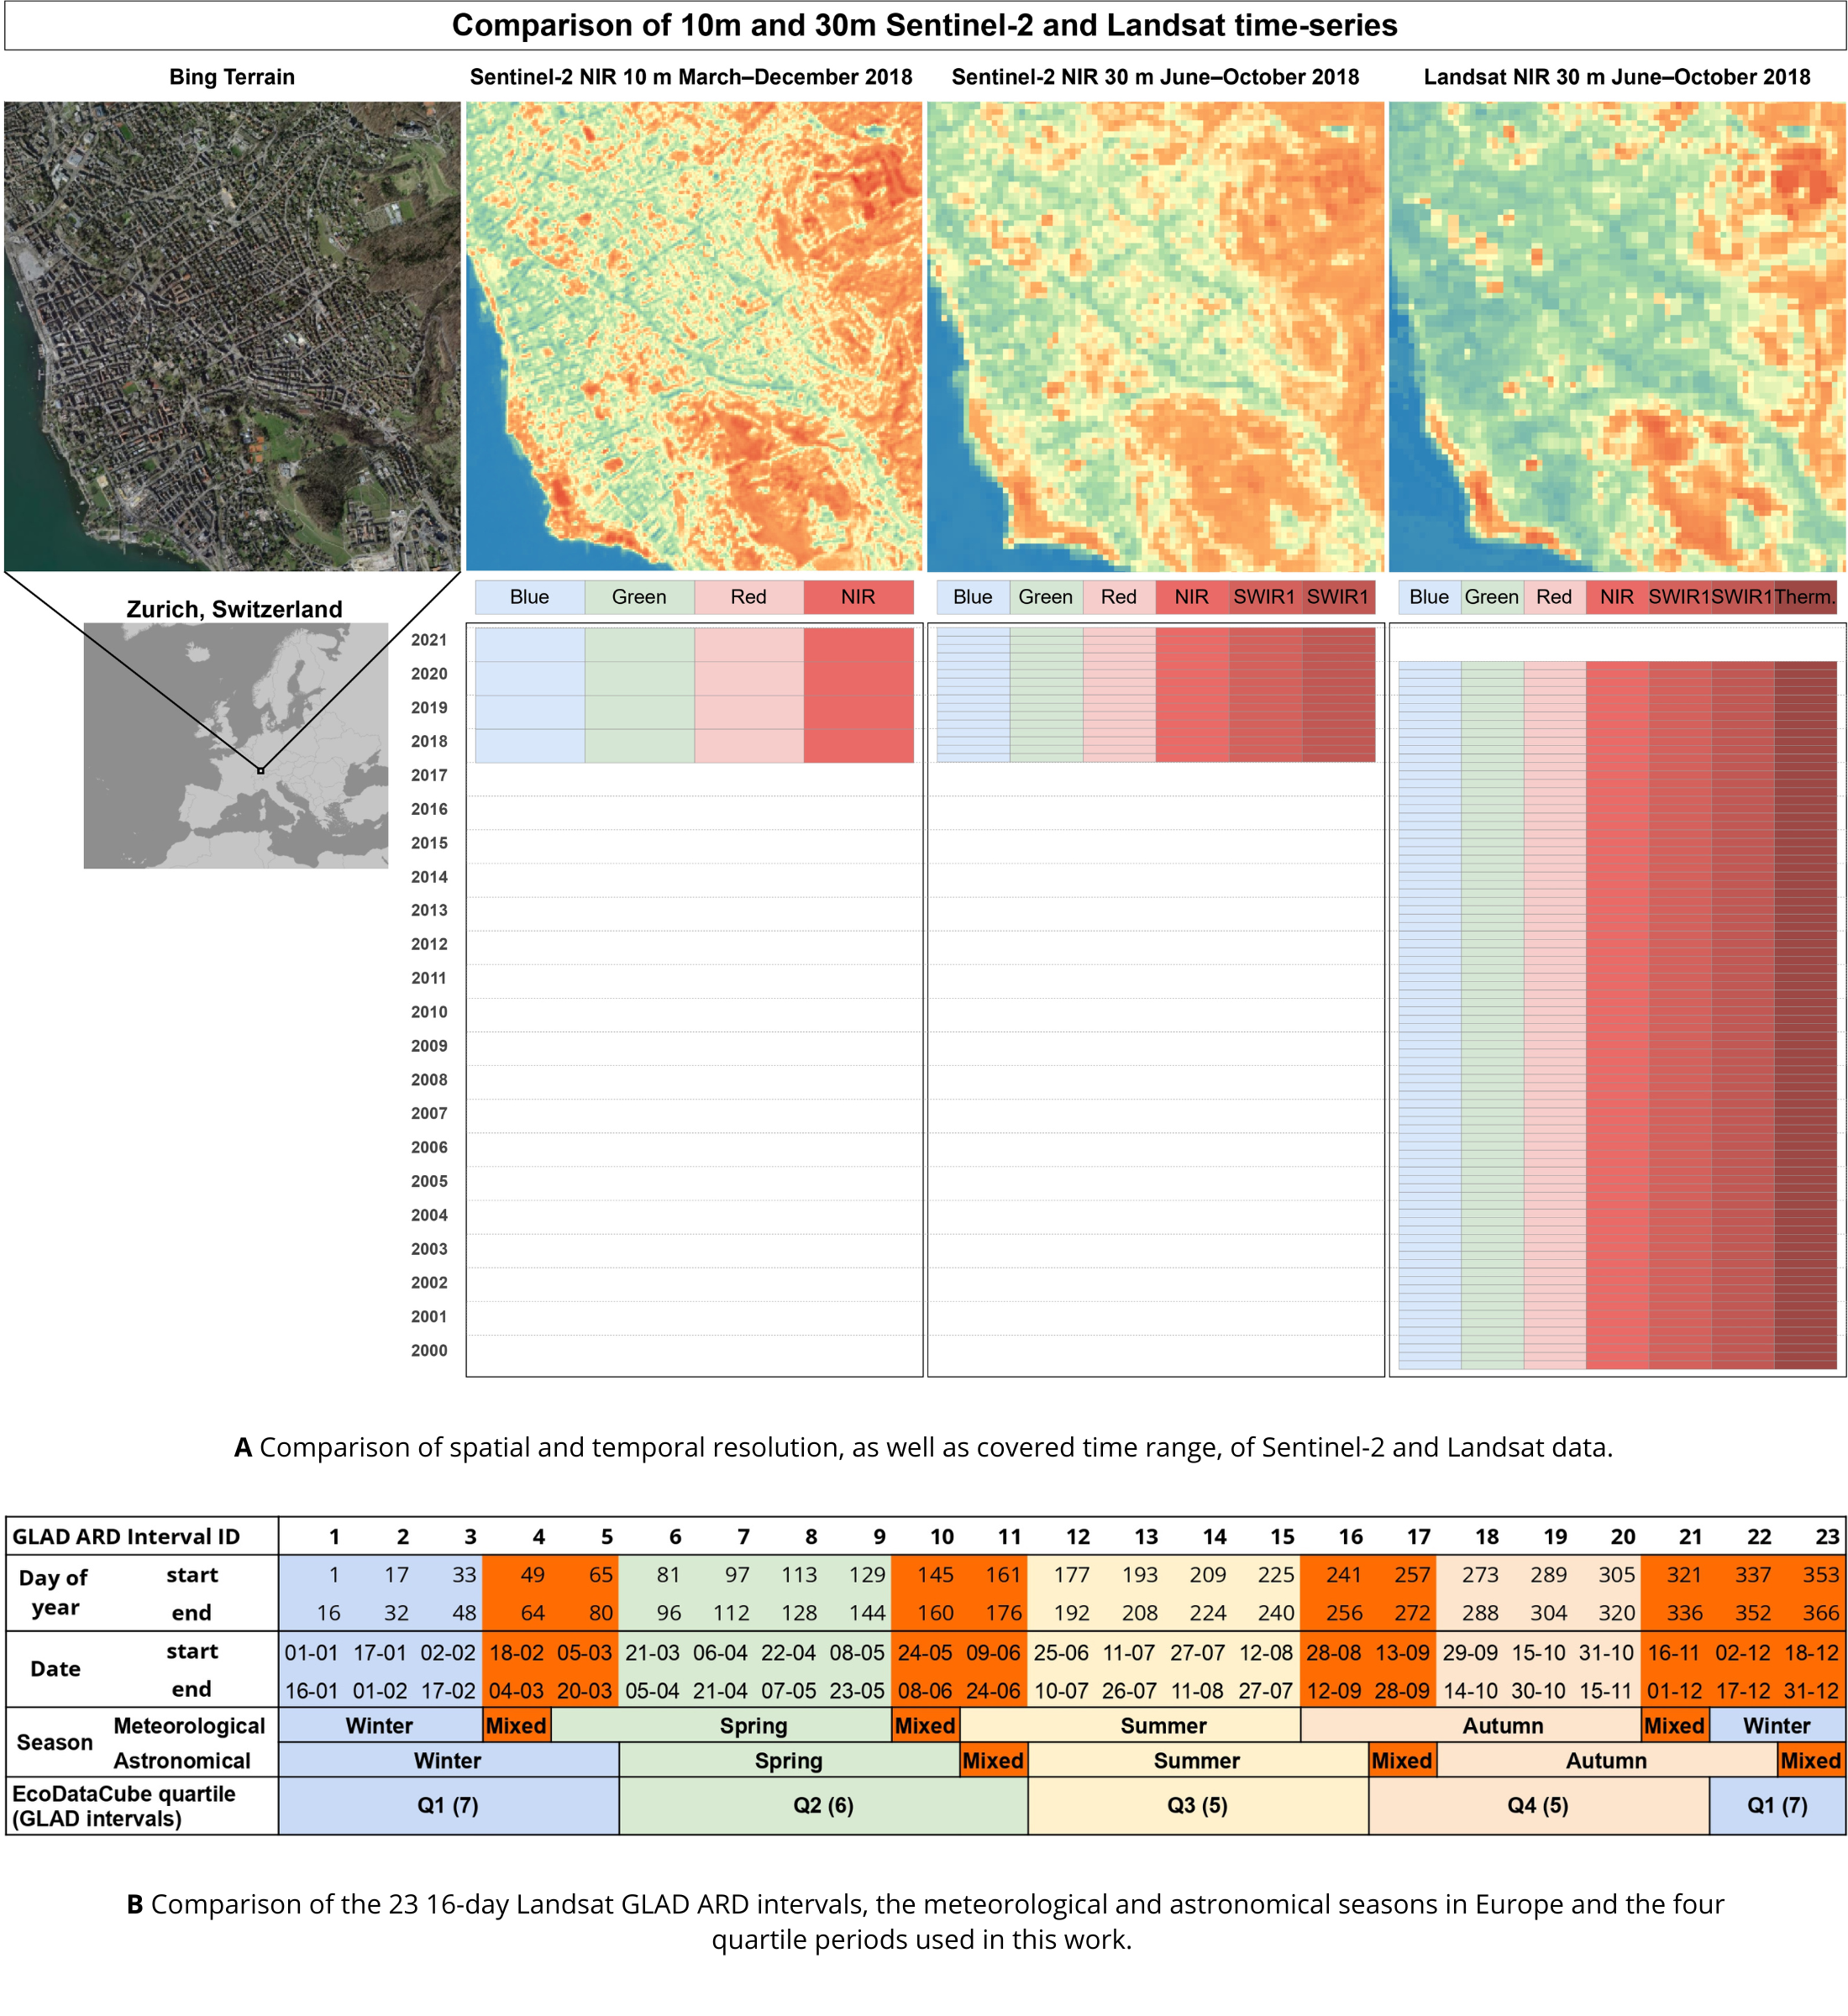
\includegraphics[width=\linewidth]{figs_02/fig_3_satellite_comparison.png}
\caption{Overview of the spatial and temporal resolution and covered time range of the presented Landsat and Sentinel-2 data. Fig.\@~A shows a comparison of the spatial and temporal resolution of the satellite imagery data sets included in EcoDataCube, as well as the available bands and time range covered per data set. Microsoft Bing Terrain screenshot \copyright~Microsoft Corporation. Fig.\@~B shows which GLAD ARD intervals were used to generate which quartiles, and how this compares to the two commonly defined seasons in Europe. GLAD ARD intervals that would be in different seasons depending on the definition are marked in bright orange.}
\label{fig:3_methods_satellite_comparison_and_intervals_seasons_quartiles}
\end{figure}

\subsubsection*{Gap-filling}

While the temporal composite aggregation reduces the number of no-data pixels in the time series at the cost of temporal resolution, gaps remain. While many gap-filling methods have been proposed, they are only well established for specific purposes (e.g. DINEOF \citep{azcarate2005dineof} for ocean modeling, Geostatistical Neighborhood Similar Pixel Interpolator \citep{zhu2012gnspi} for Landsat 7 Scan Line Corrector-off images), too computationally intensive to process multi-decade, continental-scale data (e.g. STAIR 2.0 \citep{luo2020stair} and linear temporal interpolation), and/or not available as maintained open source software. 

In order to impute these remaining missing values in this multi-decade, continental-scale data set, we developed and implemented a custom gap-filling method: Temporal Moving Window Median (TMWM). The algorithm is designed to be computationally fast and suitable to gap-fill data for annual mapping for machine learning. It therefore only uses existing values in the data set instead of estimated values like averages or linear inter- and extrapolations, which makes sure that any imputed values are from the same feature space subsequent models are trained on. It fills gaps in a pixel by deriving median pixel values from its `temporal neighbours'. If the same pixel has a value for the same period in the next and/or previous year, TMWM takes the median of that period in the two `adjacent' years. If the pixel had no value in the same period of the previous or next year, the `window' expands to include values for that period in increasingly earlier and later years. If no value exists for the specified period in any year, TMWM will derive the pixel's median value in the previous and next period of the same year. If that fails, the `window' will again expand to include the previous and next period of increasingly earlier and later years. If no value can be found in these ways, the window encompasses all values in the entire time series of the pixel. If the pixel lacks data throughout the entire time series, the value is imputed with a local spatial average and assigned a QA value of 100.

TMWM attempts to derive a value for missing pixels in three phases. Within each phase, it will first try to use only eligible values within the last X and subsequent X years, where X is half the window size. If that fails, it will try to use values within double the search range. Then, it will try to use eligible values from any year in the time series. If that yields no result, it will move to the next phase, increasing the number of eligible values by including more intra-annual time periods in its search. These phases differ in which metric they calculate and which periods they use in the following way:

\begin{enumerate}[noitemsep]
\item The median of the same period from different years;
\item An average of the medians of the previous and next periods;
\item The median of all periods.
\end{enumerate}

We validated TMWM's performance on the temporal composite Landsat data from 2000 to 2020. This was done by sampling 100 pixels from each 6,750 30~km tiles and extracting the time series for the 50th percentile of each band and each period. If tiles were not completely covered by land, the number of sampled pixels was reduced in proportion. We then created a boolean mask based on whether the pixel had a value in that year. This `missing value mask' was then inverted in order to introduce additional simulated gaps, reproducing existing patterns in which missing values occur in the data. We then used the TMWM method to fill the simulated gaps, and compare the imputed values to the original values. We quantified the performance of TMWM by deriving the root mean square error (RMSE) for each band and quartile. As different bands have different value ranges, we normalized the RMSE per band by dividing it by the range (maximum value minus minimum value) of that band's values in the entire data set. This normalized RMSE (NRMSE) allows for a standardized comparison of performance across bands and years.

\subsection*{Sentinel-2}

We created two Sentinel-2 2018--2021 time series of the study area: one series with annual values at 10~m resolution limited to the red, green, blue, and NIR bands, and one quartile/seasonal series at 30~m resolution which also includes the SWIR1 and SWIR2 bands. The data was processed in four steps (Fig.\@~\ref{fig:2_study_area_satellite_input}-E):
\begin{enumerate}
\item Computing temporal composites (annual and quarterly) for each Sentinel-2 tile;
\item Reprojecting and resampling the tiled composites to \texttt{EPSG\:3035} (\url{https://epsg.io/3035}) at 10~m and 30~m resolution;
\item Mosaicking the resampled composites over their respective orbital tracks;
\item Stitching the orbital mosaics together.
\end{enumerate}

The Sentinel-2 mosaics were built from Sentinel-2 Level 2A (S2L2A) imagery (BOA reflectance generated with scene classification and atmospheric correction algorithms), for six bands (see Table\@~\ref{tab:s2_bands}). The mosaics span 1,028 tiles. Each scene over these tiles, imaged over the time period from winter 2017/2018 (2.12.2017) to winter 2020/2021 (1.12.2021), was collected from the AWS Sentinel-2 repository, which is hosted as a Requester Pays S3 bucket (accessible without charge from AWS instances). The mosaicking and temporal aggregation was performed with the \emph{s2mosaic} functionality of the \emph{eumap} python package \footnote{Code is available at \url{https://gitlab.com/geoharmonizer_inea/eumap/-/tree/master/eumap/data sets/eo/s2mosaic}, documentation at \url{https://eumap.readthedocs.io/en/latest/notebooks/09_sentinel2_mosaicking.html}}

\begin{table}[hbt]
\centering
\caption{Sentinel-2 bands included in the data cube with their respective wavelengths and original imaging resolutions}
\label{tab:s2_bands}
\begin{tabular}{@{}cccc@{}}
\hline
Band number & Band name & Wavelength (nm) & Resolution (m) \\
\hline
B02 & Blue & 496.6--492.1 & 10~m \\
B03 & Green & 560--559 & 10 m \\
B04 & Red & 664.5--665 & 10 m \\
B08 & NIR & 835.1--833 & 10 m \\
B11 & SWIR1 & 1613.7--1610.4 & 20 m \\
B12 & SWIR2 & 2202.4--2185.7 & 20 m \\
\hline
\end{tabular}
\end{table}



\subsubsection*{Sentinel Temporal Composites}

We created annual composites of the four 10~m resolution Sentinel-2 bands: green, blue, red, and NIR. We aggregated all scenes captured between March 21st and December 1st to three percentiles: 25th, 50th (median) and 75th, excluding all pixels flagged in the S2L2A cloud and cloud shadow masks. These were then resampled to \texttt{EPSG:3035}. We also created quarterly percentile composites of all bands (green, blue, red, NIR, SWIR1, and SWIR2) with date ranges matching the Landsat quartile periods. The tile-wise composites were resampled to 30~m resolution in \texttt{EPSG:3035} and aggregated to the same quartiles as the Landsat ARD data. Since scenes that are acquired along the same orbital track are very likely to be imaged in equivalent conditions, seamless mosaicking is possible by averaging the overlapping pixels. A total of 32 orbital tracks were used (Fig.\@~\ref{fig:2_study_area_satellite_input}-D). The final mosaicking was done by stitching together the orbital mosaics with weighted averaging of overlapping pixels. For each pair of overlapping pixels, the relative distance from their respective orbital track was calculated (from 0 to 1, with 1 being the distance to the neighboring track). Overlapping pixels with a relative distance within the range of 0.4 to 0.6 (inclusive) were averaged by using their relative distances as weights, while pixels with a relative distance below 0.4 were designated the correct value, regardless of overlap, as artifacts were often observed at relative distances above 0.6. 

\subsection*{Digital Terrain Model}

Although a continental-scale DTM called \emph{``EU-DEM''} already exists, it is based on SRTM and ASTER GDEM \citep{jozsa2014evaluation}; we have built a DTM for the study area using more detailed and more up-to-date elevation products: MERIT DEM \citep{yamazaki2019merit}, ALOS AW3D \citep{takaku2018quality} and GLO-30 (\url{https://doi.org/10.5270/ESA-c5d3d65}). To generate the best estimate of the land surface/terrain elevation, we used 10 input variables, obtained by overlaying the training points on 5 elevation and 5 auxiliary raster data sets (Table~\ref{tab:input-for-dtm}), and an ensemble machine learning approach trained on a random sample of 7~million (randomly sampled from the 28 million points available) Global Ecosystem Dynamics Investigation (GEDI) points and 2~million ICESat-2 points. We specifically used GEDI level 2B points \verb"elev_lowestmode" column and ICESat-2 (ATL08) \verb"h_te_mean" column, which in both cases represent the \emph{lowest} elevation observed i.e.\@ the most likely bare ground height. We combined these two ground-truth data sets in a total of 9~million data points, and then built a machine learning model that we used to predict height without canopy and report predictions errors.

The ensemble model was composed of a random forest, a cubist model, and a generalized linear model in the \textsf{mlr} R package. These models make separate predictions using all input variables. Their estimates are then used as input for the \texttt{makeStackedLearner} meta-learner function \citep{bischl2016mlr}; in this case a linear regression model that makes the final elevation estimate for each pixel. This approach can be compared to the approach of \citet{hawker202230} who produced a global map of elevation with forests and buildings removed, however, in our approach we also use continental data set EU-DEM and numerous additional layers, at the cost of higher complexity and computational effort. We also validated the four DEMs used as input for the ensemble by comparing their values with the GEDI/ICESat-2 training data set, which can be considered ground-truth data.

Note that the predicted elevations are based on the GEDI data, hence the reference water surface (WGS84 ellipsoid) is about 43~m higher than the seawater surface for a specific EU country. Before modeling, we corrected the reference elevations to the Earth Gravitational Model 2008 (EGM2008) by using the 5-arcdegree resolution correction surface \citep{pavlis2012development}. 

We assessed the accuracy of the ensemble model and the resulting DTM by performing $k$-fold spatial cross-validation \citep{lovelace2019geocomputation}. We divide the study area into square blocks of 30{\texttimes}30~km, which are grouped to provide folds for the cross-validation approach. Because the publications describing the input DSMs do not report accuracy with comparable metrics or criteria, we also validated each input data set with our training/cross-validation data set i.e.\@ by using the GEDI and ICESat-2 points. This provides an objective comparison between each input DTM, and the cross-validation predictions of the ensemble. The produced Ensemble DTM of Europe and prediction errors were provided as GeoTIFFs using Integer format (elevations rounded to 1~dm) and have been converted to Cloud Optimized GeoTIFFs using GDAL 3.1.4.

\begin{table}[t]
\caption{Overview of data sets used as input for the ensemble that produced our DTM}
\label{tab:input-for-dtm}
\resizebox{\linewidth}{!}{%
\begin{tabular}{lll}
\hline
Dataset                     & Producer                                                  & Source                        \\
\hline
MERIT DEM                   & University of Tokyo Global Hydrodynamics lab              & \citep{yamazaki2017high}      \\
EU-DEM                      & European Environmental Agency (EEA)                       & \citep{mouratidis2019european}\\
ALOS AW3D0                  & JAXA Earth Observation Research Center (EORC)             & \citep{tadono2014precise}     \\
GLO-30                      & European Space Agency (ESA)                               & \citep{glo30}                 \\
Canopy Height               & UMD GLAD                                                  &  \citep{potapov2021mapping}   \\
Surface Water Probability   & European Commission Joint Research Centre (JRC)    & \citep{pekel2016high}         \\
Tree Cover                  & Global Forest Watch                                       & \citep{hansen2013high}        \\
Bare ground cover           & UMD GLAD                                                  & \citep{hansen2013high}        \\
Pan-European Land cover     & Humboldt University of Berlin                             & \citep{pflugmacher2019mapping}\\
\hline
\end{tabular}
}%
\end{table}

\subsection*{Land Cover Classification Experiments}

Because the intended purpose of the presented data sets is to facilitate annual mapping with machine learning, we compare the usefulness of 30~m Landsat, 30~m Sentinel-2, and 10~m Sentinel-2 for land cover classification. We do this by training several Random Forest (RF) models on 300,543 observations from the European Land Use and Land Cover Survey (LUCAS) data set harmonized by \citet{d2020harmonised} to predict the 8 LUCAS level-1 land cover classes; each of these RF models uses a different combination of the feature space provided by the data cube (Sentinel-2 10~m and 30~m, Landsat, and DTM).  Additionally, to investigate the added value of the multi-decade harmonized Landsat time series, we trained RF models on all 1.4~million available LUCAS observations from 2000--2020. 
For each classification task we used a RF classifier with 100 trees, 1 minimum sample per leaf, and 2 minimum samples per node, implemented in Python 3.8.6  using Scikit-Learn . The maximum number of features per tree was set to the square root of the amount of total features. We assess the performance of each model through both 5-fold cross-validation on its training set, and by validating each model on one randomly sampled left-out test data set of 33,394 LUCAS observations from 2018 and 2019. The different combinations of time range, data set usage, and train/test points are presented in Table~\ref{tab:landcover_experiments_methods}. 

\begin{table}[!hbt]
\centering
\caption{Overview of land cover classification experiments that were performed to quantify the added value of each data set to the data cube.}
\label{tab:landcover_experiments_methods}
\begin{tabular}{@{}llllr@{}}
\hline
Satellite    & Resolution & Time range & DTM used & Training points \\ 
\hline
Landsat    & 30~m        & 2000--2020  & Yes              & 1,443,227 \\
Landsat    & 30~m        & 2000--2020  & No               & 1,443,227 \\
Landsat    & 30~m        & 2018--2021  & Yes              & 300,543   \\
Landsat    & 30~m        & 2018--2021  & No               & 300,543   \\
Sentinel-2 & 30~m        & 2018--2021  & Yes              & 300,543   \\
Sentinel-2 & 30~m        & 2018--2021  & No               & 300,543   \\
Sentinel-2 & 10~m        & 2018--2021  & Yes              & 300,543   \\
Sentinel-2 & 10~m        & 2018--2021  & No               & 300,543   \\ 
Sentinel-2 & 10~m + 30~m  & 2018--2021  & Yes              & 300,543   \\
Sentinel-2 & 10~m + 30~m  & 2018--2021  & No               & 300,543   \\
Landsat + Sentinel-2 & 30~m        & 2018--2021  & Yes    & 300,543   \\
Landsat + Sentinel-2 & 30~m        & 2018--2021  & No     & 300,543   \\
Landsat + Sentinel-2 & 10~m + 30~m  & 2018--2021  & Yes    & 300,543   \\
Landsat + Sentinel-2 & 10~m + 30~m  & 2018--2021  & No     & 300,543   \\
\hline
\end{tabular}
\end{table}


\section*{Results}

\subsection*{Landsat}

Downloading the 2000--2020 time-series of 16-day composites for 1,149 1--degree GLAD geotiffs of 72.3GB each amounted to approximately 81~TB of data, or 1~TB per band and year. Compressing the scaled long integer values to Byte format and aggregation into temporal composites reduced this to 29~GB per band per year, constituting a size reduction of about 97.1\%. Removing all pixels not labeled as having \emph{``clear sky''} in the GLAD metadata, resulting in an average of 5.83\% empty pixels in spring, 19.7\% in summer, 11.73\% in autumn, and 54.29\% in winter, when aggregated to quarterly temporal resolution. Fig.\@~\ref{fig:4_gaps_landsat} shows that, on average across all years, more gaps occur in Scandinavia and the northern Baltic countries. Fig.\@~\ref{fig:4_gaps_landsat}-E shows that the winter quartile of each year consistently had the highest number of gaps, followed by summer in all years except 2003. It also shows a clear reduction in gaps after the winter of 2012--2013 and the inclusion of Landsat-8 data in the archive. 

%f
\begin{figure}[!hbt]
    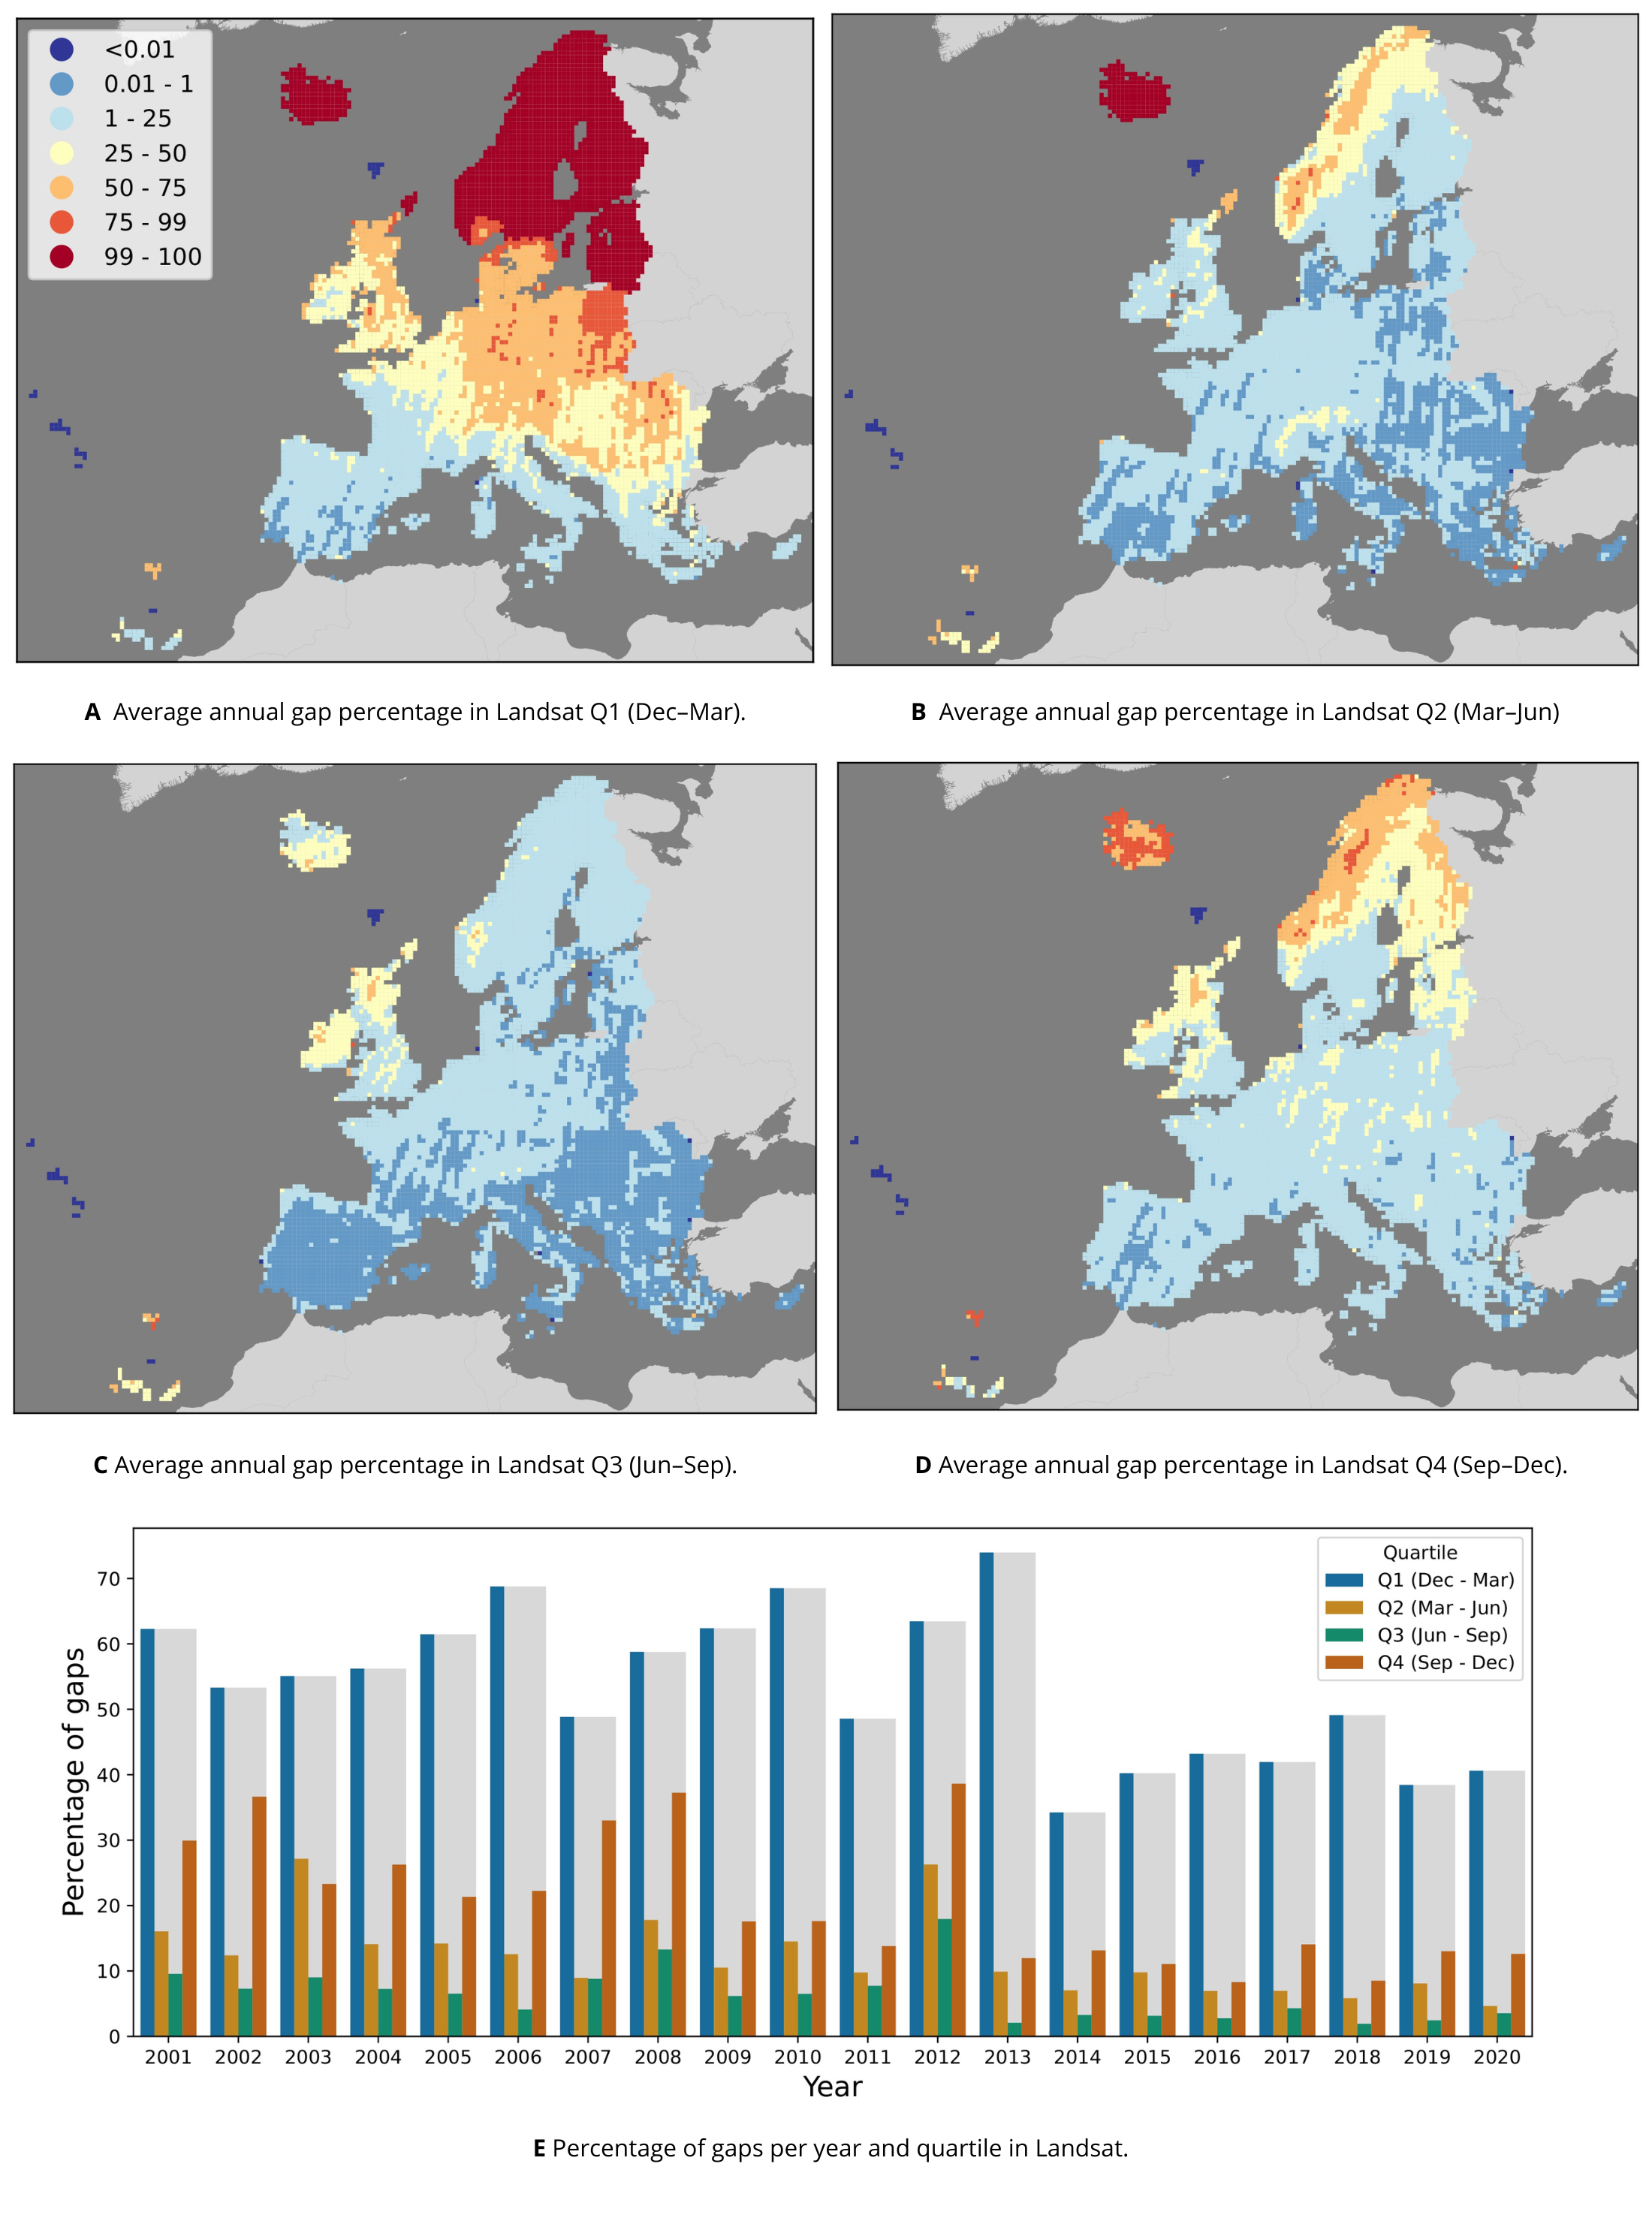
\includegraphics[width=\linewidth]{figs_02/fig_4_gaps_landsat.png}
    \caption{Percentage of gaps per pixel in the Landsat 30~m data between 2000--2020. Figs. A, B, C and D show the annual average, calculated per 30~km tile (1~million pixels) for each of the four quartiles that the GLAD Landsat ARD product was aggregated to. Fig.\@~E shows the percentage per year and quartile.}
    \label{fig:4_gaps_landsat}
\end{figure}

Sampling 100 gap-filling validation pixels for each 30~km tile in proportion to its land area resulted in 566,454~pixels from 6,750~tiles. Table\@~\ref{tab:results_gap-filling_nrmse} shows the average gap-filling NRMSE respectively per band and quartile. Our validation shows that the lowest gap-filling performance was on the NIR band in Q2 (Spring) with a NRMSE of 4.41\%, while the thermal band in Q2 was filled the most accurately with a NRMSE of 0.66\%. More generally, Q3 (Summer) was gap-filled the most accurately with an average NRMSE of 2.09\% , while Q4 (Winter) was gap-filled the least accurately with an average NRMSE of 2.36\%. Fig.\@~\ref{fig:5_map_gap-filling_nrmse} shows the spatial variability of gap-filling NRMSE per quartile, indicating a consistent higher error rate in mountainous areas, especially the Alps and the Scandinavian mountains.

\begin{figure}[!t]
    \centering
    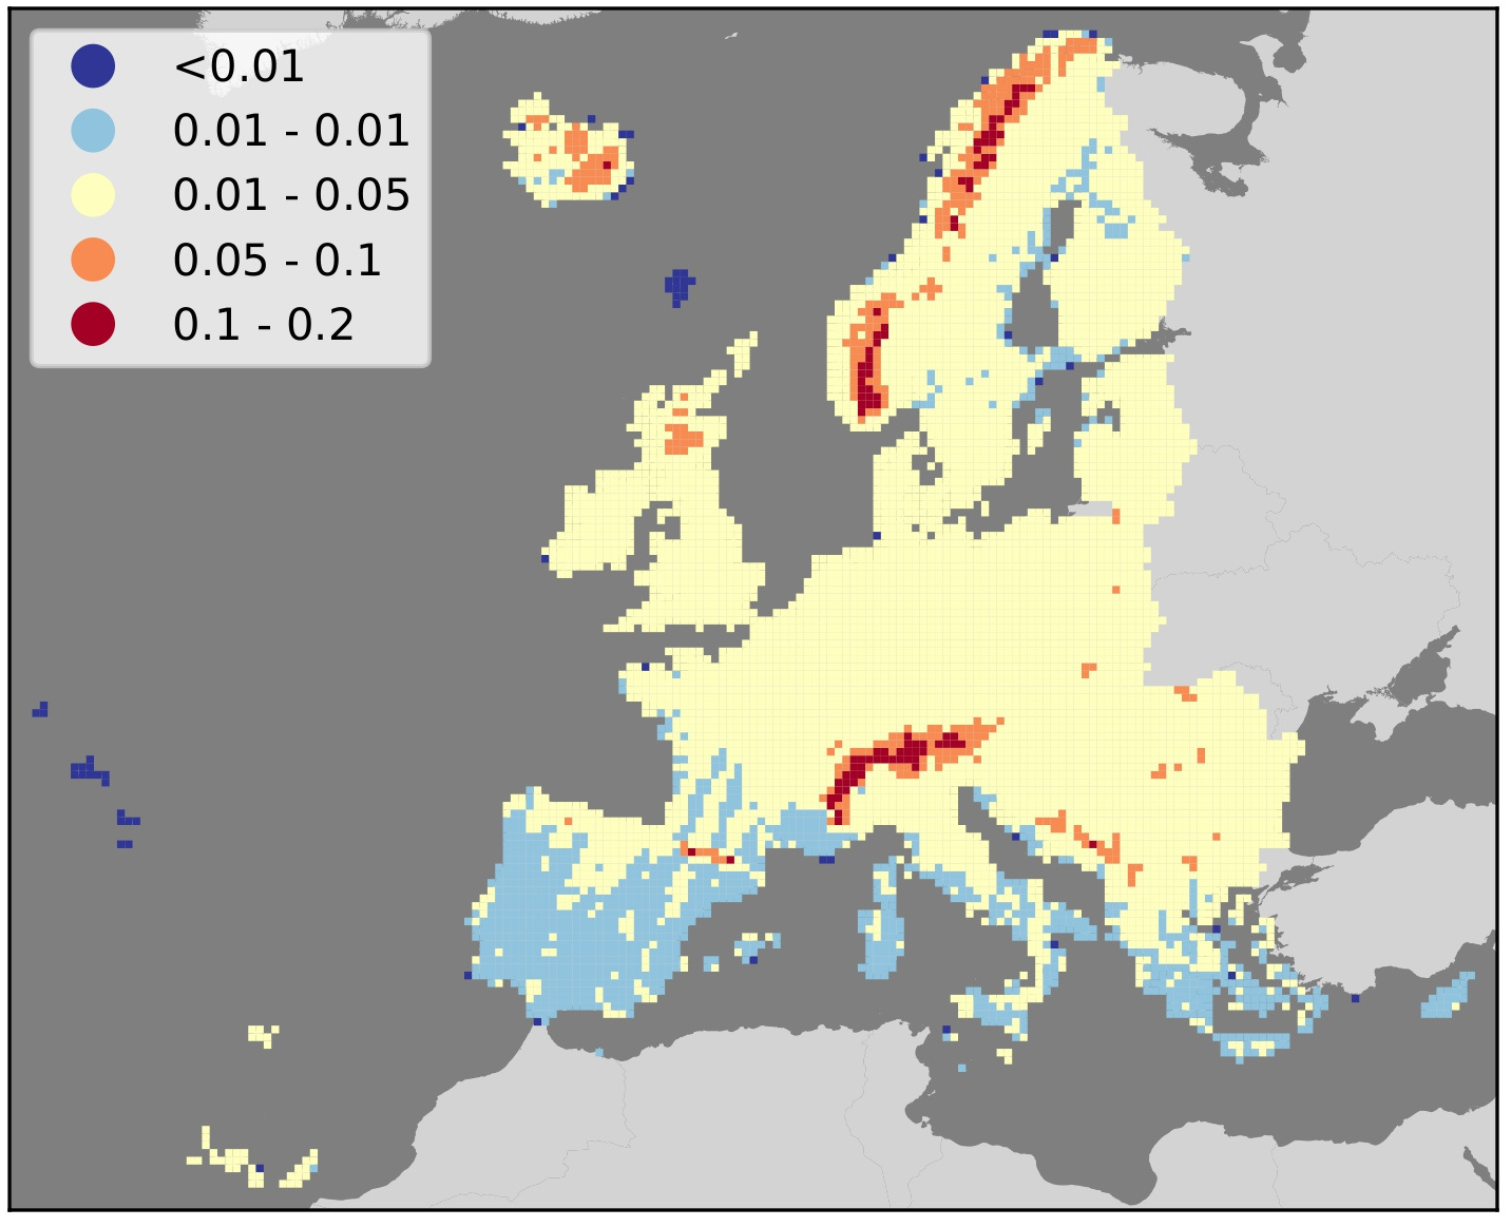
\includegraphics[width=0.6\linewidth]{figs_02/fig_5_gapfilling_accuracy_landsat.png}
    \caption{Map of average gap-filling NRMSE per 30~km tile in the study area. Results show consistently higher values in mountainous regions, and lower values in Southern Europe.}
    \label{fig:5_map_gap-filling_nrmse}
\end{figure}

\begin{table}[h!]
\centering
\caption{gap-filling validation NRMSE (in percentage) per band and quartile, as well as band \& quartile averages.}
\label{tab:results_gap-filling_nrmse}
\begin{tabular}{lrrrrr}
\hline
Band    & Q1 (Winter)  	& Q2 (Spring) 	&  Q3 (Summer) 	&  Q4 (Autumn) 	&  Average \\
\hline
Blue    &    2.10 		&    1.79 		&    1.84 		&    2.15 		&     1.97 \\
Green   &    1.64 		&    2.03 		&    1.65 		&    1.99 		&     1.83 \\
Red     &    2.37 		&    2.25 		&    2.30 		&    2.03 		&     2.24 \\
NIR     &    3.74 		&    4.41 		&    3.69 		&    4.34 		&     4.05 \\
SWIR1   &    2.46 		&    2.88 		&    2.43 		&    2.92 		&     2.67 \\
SWIR2   &    2.20 		&    2.18 		&    2.08 		&    2.37 		&     2.21 \\
Thermal &    0.68 		&    0.66 		&    0.67 		&    0.71 		&     0.68 \\
Average &    2.17 		&    2.31 		&    2.09 		&    2.36 		&     2.23 \\
\hline
\end{tabular}
\end{table}


\subsection*{Sentinel-2}

A total of 190,884 Sentinel-2 scenes were processed, ranging from 13 to 119 scenes per tile and quartile (see Table\@~\ref{tab:s2_scenes}), amounting to a data set size of roughly 15.5~TB per quartile, or 62~TB per year. The input data for each annual composite of Sentinel-2 10~m RGB+NIR was an average of 62~TB per year. Aggregating them to annual composites reduced the size to roughly 0.3~TB per band, or 1.2~TB for the four bands, resulting in 98.1\% compression. The 10~m resolution product had an average of 0.397\% gaps per year, with the median among 30~km tiles being 0\%. Fig.\@~\ref{fig:6_gaps_sentinel} shows that most 30~km tiles with gap percentages above 0.1\% occur on tiles next to water. 

\begin{table}[!hbt]
\centering
\caption{Number of Sentinel-2 scenes processed per Sentinel-2 tile and quarter}
\label{tab:s2_scenes}
\begin{tabular}{@{}lllll@{}}
\hline
Quartile & Max & Min & Mean & Standard Deviation \\ 
\hline
Q1 (Winter) & 84 & 16 & 47.95 & 11.82 \\
Q2 (Spring) & 119 & 19 & 53.07 & 17.49 \\
Q3 (Summer) & 100 & 16 & 43.87 & 14.65 \\
Q4 (Autumn) & 81 & 13 & 40.07 & 10.38 \\
\hline
\end{tabular}
\end{table}

The input data for each annual set of Sentinel-2 quarterly composites at 30~m RGB+NIR+SWIR were identical to those used for the annual 10~m composites, amounting to an average of 62~TB per year. Aggregation to quarterly composites reduced the size to 0.2~TB per quarter, or 0.8~TB yearly, resulting in a compression of 98.7\%. 

Fig.\@~\ref{fig:6_gaps_sentinel}-E shows that most gaps occur each year in the first quarter, especially in 2018. Except in 2018, the second highest number of gaps occurred in quarter 4 (September-December). Figs.\@~\ref{fig:6_gaps_sentinel}-A--D shows that across all years, Northern Scandinavia has the least gaps in quarter 2 (March-June), and that relatively more gaps occurred in a stripe pattern across Europe in quarter 1 (December-March).

\begin{figure}[!hbt]
    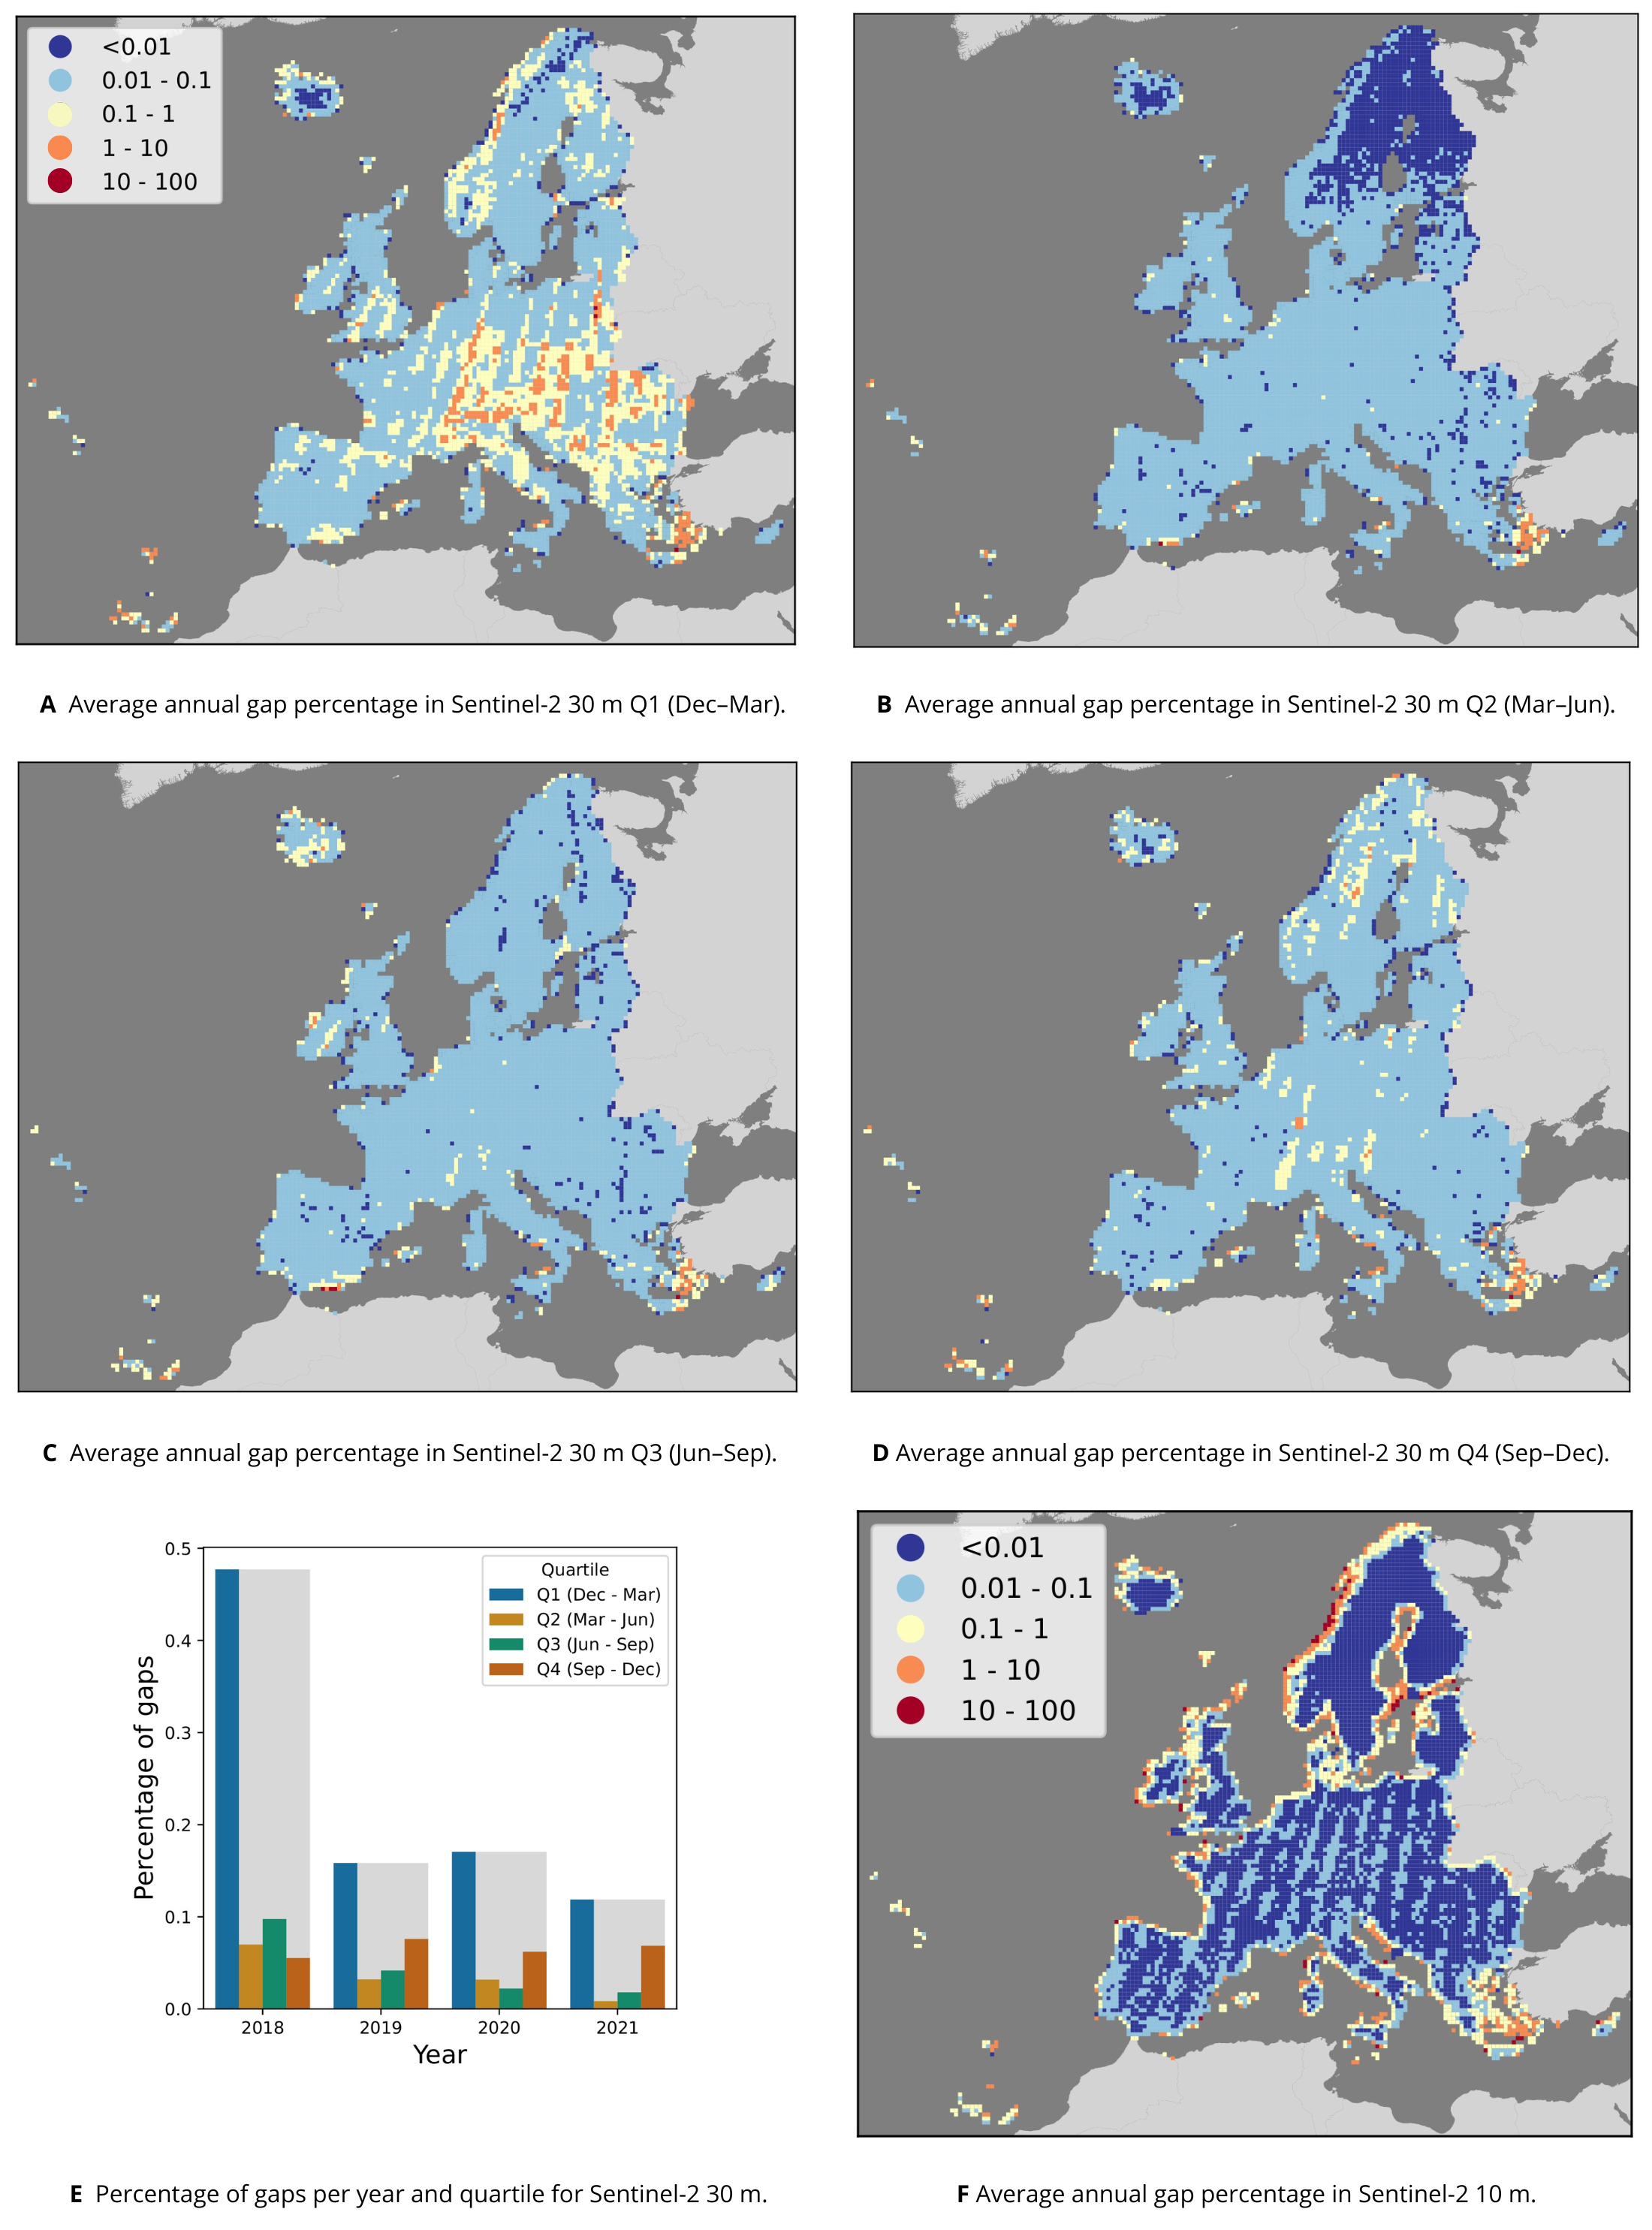
\includegraphics[width=\linewidth]{figs_02/fig_6_gaps_sentinel.png}
    \caption{Overview of gaps per pixel in the Sentinel-2 time series. Average annual percentage of gaps per quartile and 30~km tile (a, b, c, d) and in total (e) for the 30~m data, as well as average annual percentage per 30~km tile for the 10~m data (f).}
    \label{fig:6_gaps_sentinel}
\end{figure}

\subsection*{Digital Terrain Model}

Results of modeling terrain with 5~million GEDI and 2 million ICESat-2 elevation measurements, using 4 existing DEMs and 6 auxiliary data sets as input variables, show a maximum cross-validation RMSE of 6.54~m for absolute accuracy of predicting terrain (bare-earth) height with majority of errors between 2--3~m (25\% and 75\% quartiles). MERIT DEM \citep{yamazaki2019merit} is the most correlated DEM with GEDI and ICESat-2 points, most likely because it has been systematically post-processed and the majority of canopy problems have been removed (Fig.\@~\ref{fig:7_dtm_comparison}). 

\begin{figure}[hbt]
\centering
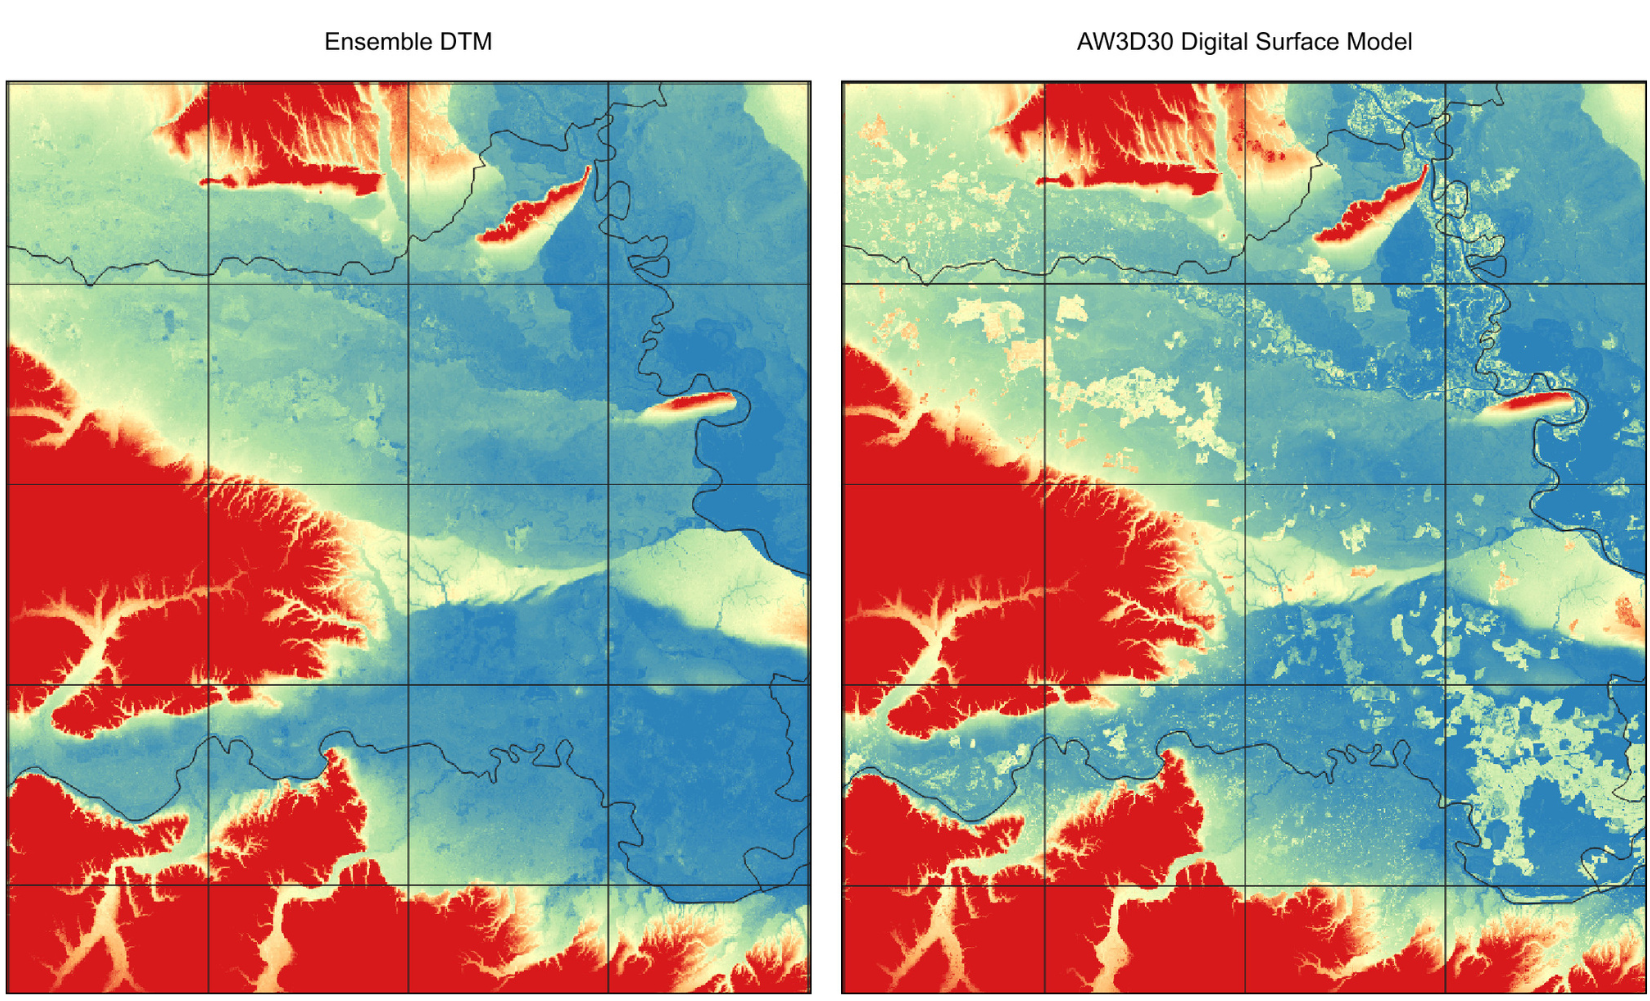
\includegraphics[width=\linewidth]{figs_02/fig_7_dtm_comparison.png}
\caption{Comparison of Ensemble DTM (left) and the AW3D Digital Surface Model for the Pannonian plane in Eastern Croatia (right). Tree height visible on AW3D seems to be systematically removed with the help of machine learning. Grid showing 30~km tiles.}
\label{fig:7_dtm_comparison}
\end{figure}

Fig.\@~\ref{fig:8_dtm_accuracy} shows the average RMSE of the four input DEMs per 30\@~km tile and the standard deviation of these four values. Our results suggest that MERIT and EUDEM are  less accurate in large parts of Sweden, while GLO30 and AW3D are less accurate in central Europe. Furthermore, red lines are visible on these maps that match GEDI orbits and no natural features. Table~\ref{tab:dem-accuracy} compares the RMSE of each DEM and the Ensemble DTM. This shows that MERIT DEM had both the lowest RMSE (8.45~m) and the highest variable importance in the model. In summary, our results show that the DTM produced by the ensemble is approximately 2~meters more accurate than MERIT in the area of interest. A copy of the all inputs, regression-matrix and outputs produced, including the code used to fit models and produce predictions, is available via \url{https://doi.org/10.5281/zenodo.4056634}.

\begin{figure}[!hbt]
    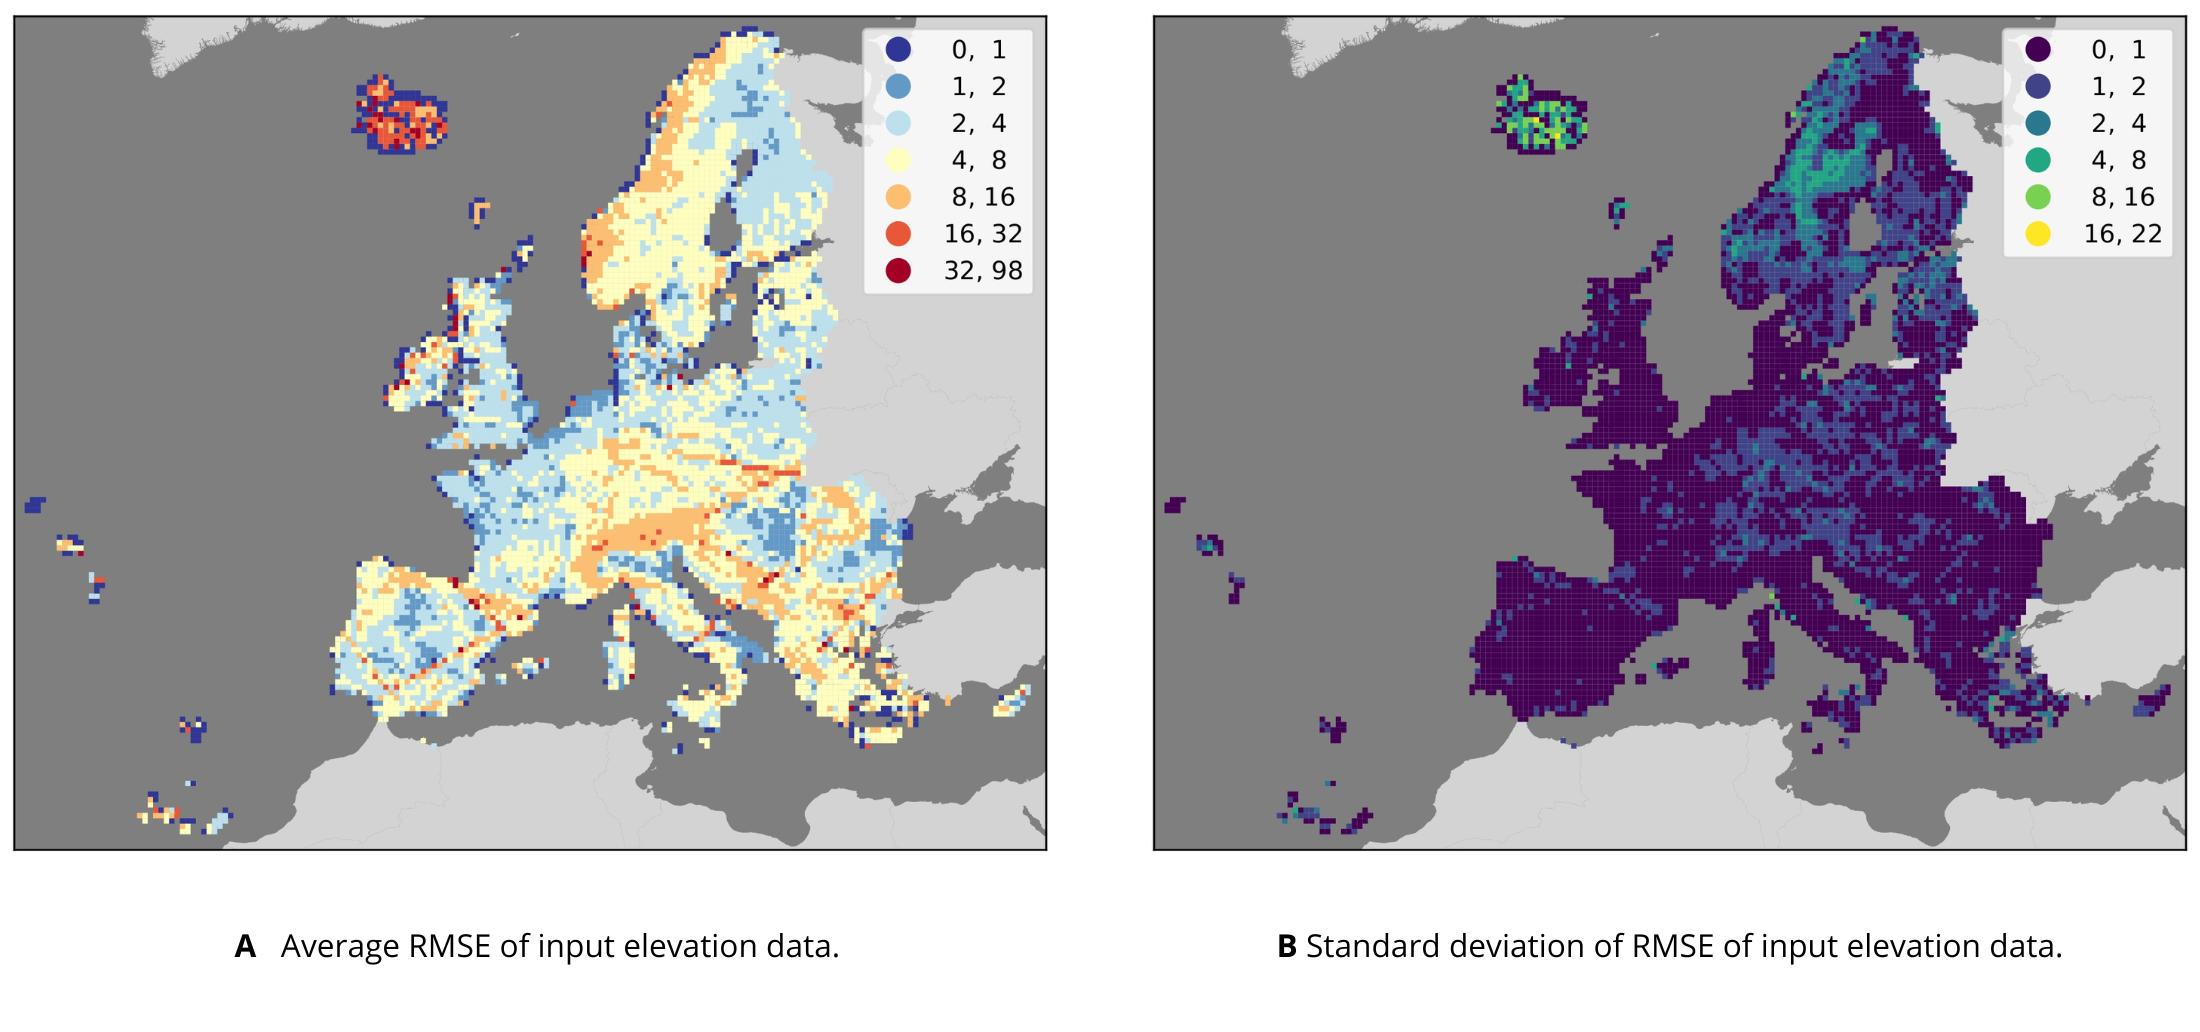
\includegraphics[width=\linewidth]{figs_02/fig_8_dtm_accuracy.png}
    \caption{Results of comparing GEDI and ICESat-2 measurements to AW3D, GLO30 EUDEM and MERIT values in 30\@~km tiles covering the study area. Fig.\@~A shows the average RMSE across the four data sets, while Fig.\@~B shows the standard deviation among RMSE values, representing the disagreement between the four data sets. Note the straight lines of higher average RMSE values in e.g. Iberia, which Fig.\@~B suggests are consistent across all four data sets. Instead, the data sets disagree most in parts of Northern Europe, especially Iceland.} 
    \label{fig:8_dtm_accuracy}
\end{figure}      

\begin{table}[hbt]
\centering
\caption{RMSE of the four input DEMs and the output DTM produced with ensemble machine learning. The RMSE of the input DEMs was acquired by comparing them to the values of 7 million GEDI/ICESat-2 points. The RMSE of the DTM was acquired through spatial cross-validation of the ensemble model. Variable importance from the random forest in the ensemble is included for the input DEMs.}
\label{tab:dem-accuracy}
\begin{tabular}{@{}lll@{}}
\hline
Dataset & RMSE  & Variable importance   \\ 
\hline
MERIT   & 8.451 & 430~B \\
AW3D    & 9.858 & 291~B \\
EUDEM   & 9.806 & 132~B \\
GLO30   & 9.900 & 201~B \\
\hline
EcoDataCube DTM & 6.544 & NA    \\ 
\hline
\end{tabular}
\end{table}

\subsection*{Land Cover Classification Tests}

The random forest utilizing all four data sets (DTM, Landsat, Sentinel-2 10~m and 30~m) achieved the highest cross-validation scores (0.761) and second-highest test score (0.767). In general, models with multiple data sets in their feature space (DTM, Landsat, Sentinel-2 at 10~m spatial resolution, and/or Sentinel-2 at 30~m) outperformed models using a single data set. However, the highest test score of 0.774 was achieved by the Landsat model trained on 300,543 LUCAS observations spread out across 2000--2020, while this model had a relatively low cross-validation score of 0.715 (see Table~\ref{tab:landcover_experiments_results}). It appears that models utilizing DTM variables achieved higher cross-validation and test F1--scores in every experiment except for the Sentinel-2 10~m model. This model also achieved the lowest cross-validation and test scores. 

Fig.\@~\ref{fig:9_landcover_feature_space} shows that models trained on data sets with multiple satellite sources and resolutions generally outperformed single-source or single-resolution models. Fig.\@~\ref{fig:9_landcover_feature_space}-A shows that \emph{``Shrubs``} and \emph{``Wetlands``} were more accurately classified by models only using 30~m data sets.  Fig.\@~\ref{fig:9_landcover_feature_space}-B shows that Sentinel-2 data was more useful for classifying \emph{``Artificial''} and \emph{``Water areas''}, while being less useful for classifying \emph{``Shrubs''} and \emph{``Wetlands''}. For these classes, Landsat data yielded higher F1-scores. Using the DTM and its derived variables generally yielded slight performance increases, except for \emph{``Crops``} and \emph{``Bare Ground``}. Fig\@~\ref{fig:9_landcover_feature_space}-A shows that including the DTM in the feature space mainly lead to higher accuracy when classifying \emph{``Shrubs''} and \emph{``Wetlands``}.

\begin{figure}[!hbt]
    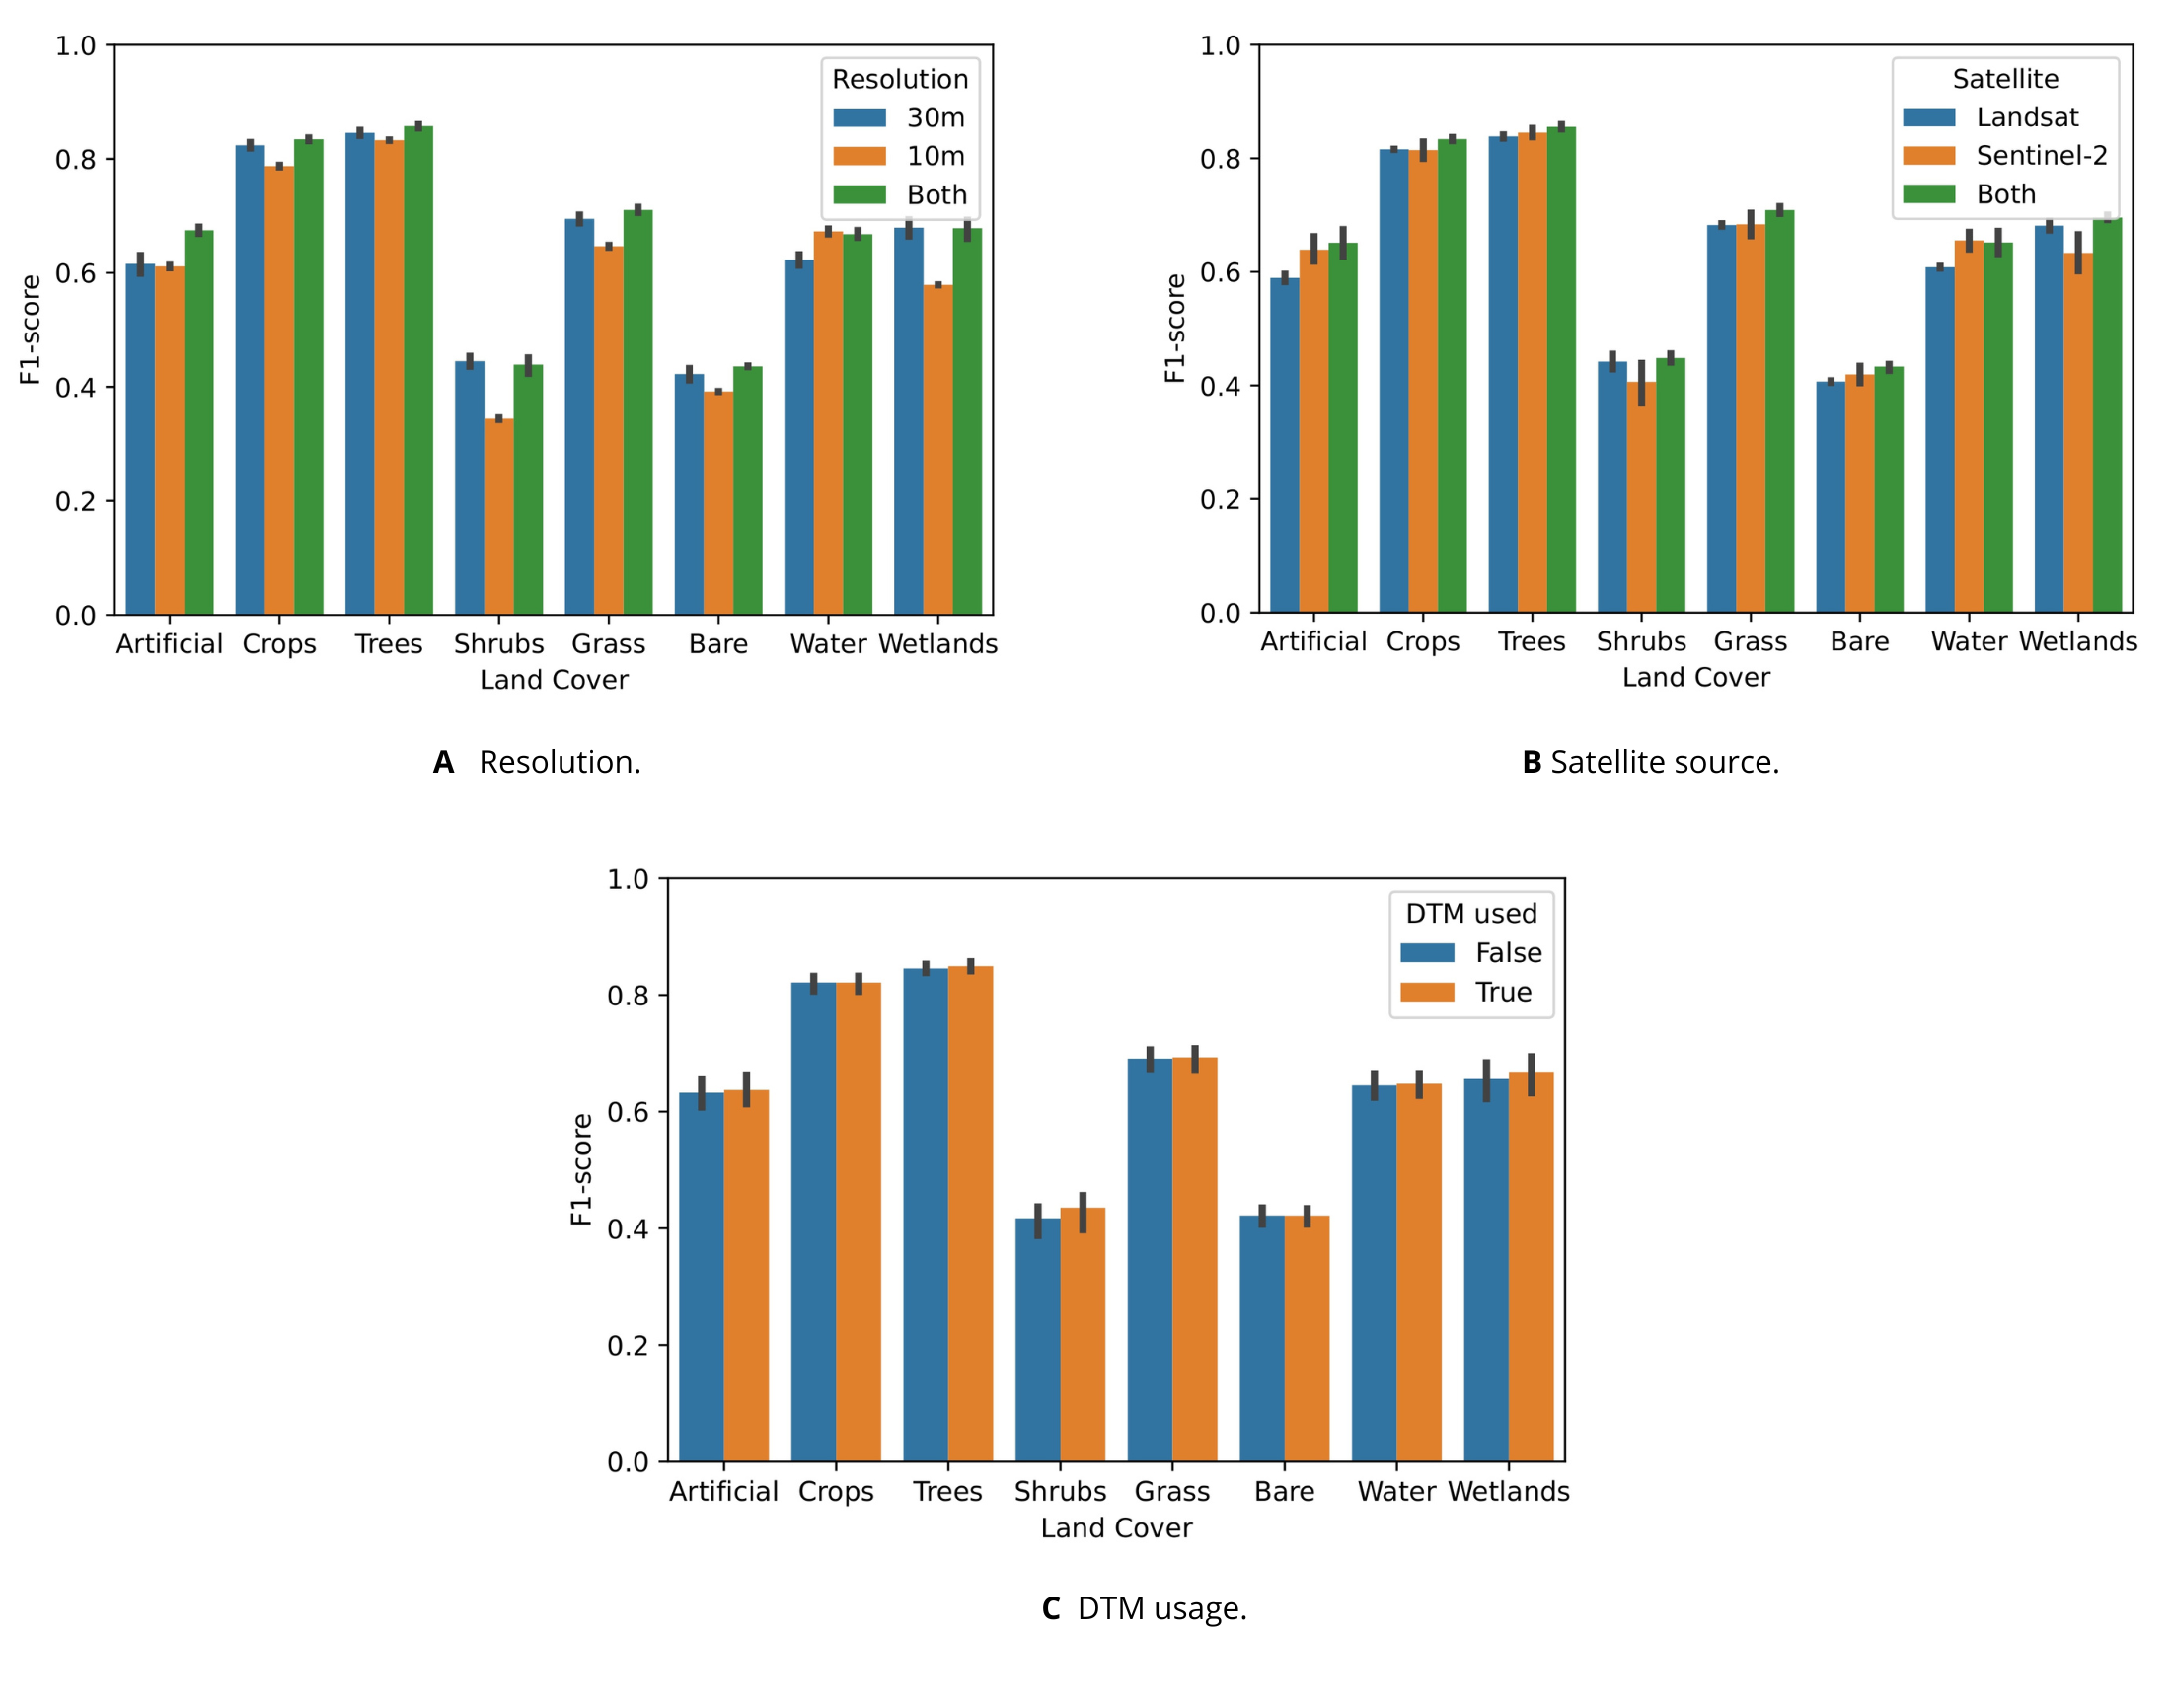
\includegraphics[width=\linewidth]{figs_02/fig_9_landcover_feature_space.png}

    \caption{Test F1-score of random forests trained to classify 8 LUCAS land cover classes, shown per class and aggregated based on which data sets were included in their feature space (A: spatial resolution, B: satellite source, and C: DTM). 
    Fig.\@~A shows that models trained on both 10\@~m and 30\@~m resolution data generally achieved the highest classification accuracy, but that models trained solely on 10~m (which is only Sentinel-2) classified water more accurately than models trained either 30m data sets or a combination of 30m and 10m. Especially the \emph{``Shrubs''}, \emph{``Grass''}, and \emph{``Wetlands''} classes were predicted much less accurately by the 10~m models. Combining 10\@~m and 30\@~m resolution data lead to the largest performance increase for the \emph{``Artificial``} class.
    Fig.\@~B shows that models trained on data from both satellite types outperformed other models on every class except \emph{``Water``}. 
    Fig.\@~C shows that models including DTM data in their feature achieved higher accuracy when classifying \emph{``Shrubs''} and \emph{``Wetlands``}.
    } 
    \label{fig:9_landcover_feature_space}
\end{figure}



\begin{table}[hbt]
\caption{Overview of land cover classification tasks that were performed to compare the usefulness of the different products, with weighted averaged F1-scores from cross-validation and from predicting on test set.}
\label{tab:landcover_experiments_results}
\resizebox{\textwidth}{!}{%
\begin{tabular}{@{}llllrll@{}}
\hline
Dataset    & Resolution & Time range & DTM  & Training points & CV F1-score & Test F1-score \\ 
\hline
Landsat    & 30m        & 2000--2020  & Yes              & 1,273,518 & 0.710 & 0.738 \\
Landsat    & 30m        & 2000--2020  & No               & 1,273,518 & 0.698 & 0.730 \\
Landsat    & 30m        & 2000--2020  & Yes              & 300,543   & 0.715 & \textbf{0.774} \\
Landsat    & 30m        & 2000--2020  & No               & 300,543   & 0.707 & 0.768 \\
Landsat    & 30m        & 2018--2021  & Yes              & 300,543   & 0.731 & 0.742 \\
Landsat    & 30m        & 2018--2021  & No               & 300,543   & 0.724 & 0.736 \\
Sentinel-2 & 30m        & 2018--2021  & Yes              & 300,543   & 0.746 & 0.753 \\
Sentinel-2 & 30m        & 2018--2021  & No               & 300,543   & 0.741 & 0.748 \\
Sentinel-2 & 10~m        & 2018--2021  & Yes              & 300,543   & 0.705 & 0.713 \\
Sentinel-2 & 10~m        & 2018--2021  & No               & 300,543   & 0.706 & 0.715 \\
Sentinel-2 & 10~m + 30m  & 2018--2021  & Yes              & 300,543   & 0.758 & 0.760 \\
Sentinel-2 & 10~m + 30m  & 2018--2021  & No               & 300,543   & 0.751 & 0.756 \\
Landsat + Sentinel-2 & 30m        & 2018--2021  & Yes    & 300,543   & 0.750 & 0.757 \\
Landsat + Sentinel-2 & 30m        & 2018--2021  & No     & 300,543   & 0.747 & 0.755 \\
Landsat + Sentinel-2 & 10~m + 30m  & 2018--2021  & Yes    & 300,543   & \textbf{0.761} & 0.767 \\
Landsat + Sentinel-2 & 10~m + 30m  & 2018--2021  & No     & 300,543   & 0.758 & 0.765 \\
\hline
\end{tabular}
}

\end{table}

%\clearpage

\section*{Discussion}

We have demonstrated a full methodological framework for processing various EO data for the purpose of producing an open Data Cube for Europe, evaluated all steps, and investigated the value of combining its component data sets using machine learning applications. Our key findings indicate that:
\begin{itemize}[noitemsep]
\item Combining all four data sets produced in this work (DTM, Landsat 30~m, Sentinel-2 30~m and Sentinel-2 10~m) yields the highest land cover classification accuracy, with different data sets improving the results for different land cover classes;
\item When used separately, the 2000--2020 Landsat data set can be used to model longer time series. In our experiments, models trained on LUCAS observations in this longer time span generalized better than those trained on an equal amount of points, but only sampled from 2018--2019;
\item Ensemble machine learning can be used as a data fusion technique to combine global elevation models and create an optimized DTM that is more accurate in the area of interest, based on an independent validation;
\item Accuracy and visual assessment of the four input DEMs suggests that DTM could still be much improved if countries would donate their national higher resolution elevation data.
\end{itemize}

In the next sections we discuss some remaining limitations of the Data Cube and suggest possible strategies to overcome them.

\subsection*{Suitability of Temporal Composite Design}

We recognize that the choice for aggregating the 23 {\texttimes} 16--day GLAD measurements into temporal composites that approximate the typical four seasons in central Europe imposes some limitations. Firstly, seasonality differs per region, even within the study area. This can cause differences in performance between regions with a matching seasonality and regions with a different one. This may be a potential explanation for the poorer accuracy of land use / land cover classification along the Mediterranean coast in \citet{witjes2022spatiotemporal}, for which this data set provided a substantial part of the feature space. Secondly, the loss of temporal resolution likely hinders the accurate classification of dynamic classes that are distinguished by intra-seasonal variation, such as different crop types \citep{vuolo2018much} or other modeling tasks involving vegetation phenology \citep{zhao2011evaluation}. However, \citet{zhao2022temporal} found that choosing an appropriate temporal compositing strategy can reduce the need for a higher temporal resolution.

While a monthly aggregation would likely help solve these issues, but would also pose new challenges: it would be more complicated to derive from the 23 measurements, as they do not perfectly match the 12 months in the Gregorian calendar. In addition, a monthly aggregation would retain more gaps in the data. While the quarterly aggregation has less temporal resolution, the three percentiles quantify some intra-seasonal variability when multiple pixel values are available per quarter. This approach retains information on the variability in the growing seasons, while reducing the lack of data in an efficient way. 

Another solution would be to use a non-symmetrical approach, where the growing season is divided into smaller time units, while the non-growing season is aggregated to a higher extent. As there are far fewer gaps in the quartiles roughly covering the growing season (Q2 and Q3, March-September; see Fig.\@~\ref{fig:4_gaps_landsat}), this approach would yield a data set that is: (1) more detailed where it matters, (2) requires less gap-filling, and (3) might be more suitable for gap-filling with TMWM. Such a technique, however, should only be used when constructing data cubes of areas with homogenous seasonal dynamics. Further research into the optimal temporal aggregation method for different subsequent modeling tasks would likely improve the usefulness of resulting data sets.

\subsection*{Gains and Limitations of gap-filling with TMWM}

The TMWM algorithm is computationally efficient and only imputes sets of existing combinations of pixel values across bands. It does have important drawbacks, however: firstly, in regions where data for a specific period is extremely sparse or non-existent (e.g. Northern Scandinavia in winter), data for this period will be almost completely derived from other periods. This can severely hamper the performance of classification tasks when a model needs intra-annual dynamics to distinguish certain classes. For example, our validation suggests that the Landsat RGB bands are easier to gap-fill with TMWM than infrared bands, especially NIR. This phenomenon is more pronounced in spring, which may be caused by the more dynamic and variable nature of vegetation in that period each year. Filling NIR data with values from other seasons may be exceptionally problematic in this respect. 

Secondly, any model trained on data using this method may be less suitable for the timely detection of changes between predicted classes. Because TMWM prioritizes previous and subsequent years when imputing missing values, the resulting feature space may stay constant while the actual situation on the ground has changed. This may make the chosen combination of temporal aggregation and gap-filling less suitable for annual change analysis. 

The \emph{qa\_f} layers included for every year and quartile at \url{https://stac.ecodatacube.eu} allow users to programmatically identify all gap-filled pixels and replace them with a gap-filling method that is optimal for their own subsequent modeling.

Finally, no gap-filling was implemented on the Sentinel-2 data sets. Although the total percentage of gaps is very low in most areas (see Fig.\@~\ref{fig:6_gaps_sentinel}, the Sentinel-2 data is not fully complete and therefore not 100\% analysis-ready.

The validation method used to assess the accuracy of the TMWM algorithm was chosen because it reproduces existing nodata patterns as observed in the intra and inter-annual dynamics of our data set, which we expect to yield to a more realistic evaluation of its performance on real-world data. However, mirroring the time-series occurrence of gaps as a validation mask simulates a larger number of missing values than their actual occurrence. Because the algorithm subsequently has less data to derive filling values with, this may lead to an underestimation of the actual accuracy.
    
\subsection*{Applicability and Limitations of Digital Terrain Model}

We validated each of the four input DTMs on the harmonized GEDI/ICESat points that we used to train our model, allowing a comparison between these data sets and with the predictions made by our ensemble. It must be noted that a thorough accuracy assessment of GEDI and ICESat-2 for generating 30~m resolution DTMS on an European scale is not available. This means that it is hard to quantify the highest attainable accuracy when using it as training data. We did notice, however, possible artifacts in the GEDI data. Fig.\@~\ref{fig:8_dtm_accuracy} shows that enough GEDI points matched poorly with each input DEM in line-shaped groups for them to cause relatively large average RMSE values in the 30~km spatial tiles. The effect is especially noticeable in Iberia, and does not match any natural features. It does, however, match the GEDI orbit track. This suggests that there might be some orbit issues affecting the local accuracy of the predictions. 

For the ensemble DTM we have produced, we noticed that in many places canopy height is still visible on the hillshading images, indicating that even after using the canopy height, the true terrain elevation in forests is overestimated. Additional filtering is needed to remove human built objects in urban areas. Our Ensemble DTM has not been hydrologically corrected and will require additional processing before it can be used for spatial modeling. Furthermore, several EU countries such as Belgium, the Netherlands, and Denmark have high-resolution terrain models built from LIDAR surveys. The 
ensemble DTM could be further improved by merging such publicly available data.  Most importantly, it should be compared with the recently published 30~m global map of elevation with forests and buildings removed \citep{hawker202230}.

\subsection*{Usefulness of EO Data for Land Cover and Land Use Mapping}

The land cover experiments, while limited in scope, clearly show that combining different data sets in the data cube improved modeling performance for classification tasks. This demonstrates the value of spatially, temporally, and spectrally harmonized multivariate data cubes such as the one presented in this work. For some of the 8 land cover classes, the combined models were outperformed by a model using only a specific data set or resolution (e.g.\@ Sentinel-2 models when classifying water areas, and 30~m resolution models when classifying wetlands).  

The different Landsat-only experiments also suggest that sacrificing spatial resolution in order to access longer time-series of training data may yield better subsequent modeling results; the 300~K 2000--2021 Landsat model outperformed the other Landsat models on the test data set. This matches findings by \citet{witjes2022spatiotemporal} and \citet{pflugmacher2019mapping}. However, the lower performance of the 1,273K 2000--2020 Landsat model suggests that using a larger training data set does not necessarily improve model performance.

Shrubland and bare land were consistently the least accurately classified land cover classes in each experiment. This was particularly the case for models trained only on 10~m Sentinel-2 data (see Fig\@~\ref{fig:9_landcover_feature_space}-A), even when taking into account their lower performance across all classes. This lower performance was likely affected by the lower number of available bands, i.e. the lack of SWIR and NIR. This possible explanation is supported by the fact that models combining 30~m and 10~m Sentinel-2 data outperformed Landsat-only models on bare land,  The model trained only on Sentinel-2 data however did outperform other models when classifying water areas, achieving a slightly higher score than even the model combining all data sources. These findings, combined with indications that the Sentinel-2 SWIR bands are highly useful for distinguishing between different tree species \citep{immitzer2019optimal} suggest that incorporating both 10~m and 30~m Sentinel-2 data sets as part of the data cube enhances subsequent land cover modeling efforts.

\subsection*{The Cost of Accessibility and Analysis-Readiness}
    
The ultimate goal of this work is to present an analysis-ready data cube that is as useful as possible to as many different users as possible, with an emphasis on time-series classification tasks. To this end, we have greatly -- sometimes by more than 90\% -- reduced the size of the input data, reduced the number of gaps to below 1\% for both Landsat and Sentinel-2 time-series, and made all products freely accessible through modern technologies and formats such as COG and SpatioTemporal Asset Catalogs (STAC) without requiring any form of user registration. However, this emphasis on accessibility and analysis-readiness comes at the cost of both temporal and spectral detail.

We aggregated a 23--part Landsat time-series and a Sentinel-2 time-series with a highly variable number of observations (13--119) into four quartiles with 3 percentiles each: a standardized total of 12 values. While this low temporal resolution approach requires less gap-filling and makes the data set less susceptible to error propagation, it may not be detailed enough to detect certain classes in some classification tasks such as those relying on vegetation phenology. Our land cover experiments did not try to distinguish between different vegetation types or inform vegetation growth models, which might only be discernible when having a higher number of observations in the growing season \citep{zhao2011evaluation}. On the other hand, \citet{vuolo2018much} present significant increases in Observer's Accuracy (OA) of crop type classification when using multi-date data, and suggest that this method alleviates the issue of finding the optimal temporal window where the highest single-date accuracy can be achieved.

We did not analyze the effects of compressing the Landsat values from long unsigned integer (0--40,000) and unsigned 16-bit integer (0--65,535), respectively, to Byte (0--255). This loss in precision may lead to similar limitations, especially in the case of infrared for vegetation-related modeling. However, \citet{bonannella2022forest} achieved high accuracy (0.81--0.89) using the Byte-scale Landsat data when classifying multiple different tree species, suggesting this may not, after all, be a significant limitation.

%f
\begin{figure}[p]
\includegraphics[width=\linewidth]{figs_02/fig_10_data_viewer.png}
\caption{Screenshot of the EcoDataCube.eu data viewer showing A: the probability of pasture land cover in 2019 near Copenhagen, Denmark, and B: Landsat-derived NDVI in the summer of 2019.}
\label{fig:10_dataviewer_pasture}
\end{figure}

\subsection*{Future Work}
    
While the EcoDataCube layers presented in this work bridge a large part of the gap between data and users through a consistent design philosophy, they are not completely finished. Notably, gaps remain in both Landsat and Sentinel-2 data. Work continues on a more efficient and effective gap-filling methodology optimized for classification tasks with probability-based post-processing such as the methodology used in \citet{witjes2022spatiotemporal}. The effects of different temporal resolutions and percentile usage will need to be compared in order to reach the optimal method for any specific task. Purely relying on time-series of the same pixel may be too limiting for areas with frequent and consistent gaps, such as Scandinavia and mountainous regions. A less stringent QA-informed removal of pixels could reduce this issue, but might require additional processing steps. Furthermore, GLAD will discontinue its current ARD Landsat archive, publishing a recomputed version that will be continued in the foreseeable future. While this necessitates a recomputation of all current EcoDataCube Landsat layers as well, it provides an excellent opportunity to compare and implement the next generation of temporal composition and gap-filling techniques.
        
The EcoDataCube platform already hosts more data sets that follow the same design philosophy of analysis-readiness and accessibility \citep{wagemann2021a}, allowing rapid and user-friendly comparisons and synthesis (see Fig.\@~\ref{fig:10_dataviewer_pasture}). Examples are the potential and realized distribution of 16 tree species \citep{bonannella2022forest}, monthly airborne fine particulate matter levels \citep{ibrahim2022machine}, 43 CORINE land cover classes \citep{witjes2022spatiotemporal}, and daily aerosol optical depth levels \citep{ibrahim2021space}. 

We aim to continuously extend the feature space of the data cube, both by producing new data sets and hosting harmonized products created by third parties. For instance, a backwards estimation of Sentinel-2 values to cover the same time period as the Landsat data set is under consideration. Data fusion approach such as the FORCE \citep{frantz2019force} provides a systematic solution for this and will likely be used for this purpose. There are thousands of data sets that could potentially be integrated in, and shared on, the EcoDataCube. For instance, with proper documentation and spatiotemporal harmonization, many of the over 1,500 data sets from the European Environmental Agency's archive (\url{https://www.eea.europa.eu/data-and-maps}) could be added to the feature space and breadth of analyses offered on the platform.

%\clearpage

\section*{Conclusions}
With the EcoDataCube data sets and platform, we present a spatiotemporally consistent, transparently and reproducibly processed continental-scale data set that is hopefully as accessible as possible across platforms. We intend it to reach the widest possible user base and to be put to as many different uses as possible --- generating more value for society --- while also facilitating collaboration and reproducibility. The intended uses of EcoDataCube include vegetation, soil, land cover and land use mapping projects, environmental monitoring by the EEA, and automated generation of data for statistical offices such as Eurostat (\url{https://ec.europa.eu/eurostat}).  
    
The EcoDataCube data sets are hosted through modern cloud-based solutions that are both humanly and programmatically accessible without limitation and with minimal effort through STAC and the EcoDataCube platform, and will be continuously updated, maintained, and expanded.

The spatiotemporal harmonization and gap-filling processes described in this work ensure that users can easily combine different data sets to perform their analyses without the need for extensive preprocessing. The included validations and published QA data sets accompanying the TMWM-gap-filled Landsat data ensure that all limitations of the data set can be easily analyzed and communicated. As we continue our work to create and host more open spatiotemporal analysis-ready data, we encourage and invite all interested parties to use these data sets and to provide feedback, especially on inaccuracies or limitations, so that these can be addressed in future versions. 

\section*{Code and data availability}
The Python code used to download the original Sentinel-2 data and GLAD Landsat archives and aggregate them into temporal composites is available at \url{https://gitlab.com/geoharmonizer\_inea/eumap} under MIT license. The code used to perform the landcover classification experiments can be found on \url{https://gitlab.com/research_m_witjes/ecodatacube}. The codebase primarily uses components of the \emph{``eumap''} python package, which is available from \url{https://eumap.readthedocs.io/en/latest/}. The accompanying Docker image can run all python code used for this paper. Data from all Landsat and Sentinel bands, quarters, and percentiles is available under a CC-BY license and can be downloaded through STAC at \url{https://stac.ecodatacube.eu}. It can also be explored and accessed through the EcoDataCube platform. All data sets are presented in the ETRS89-extended / LAEA Europe projection (\texttt{EPSG:3035}).


	\chapter[Spatiotemporal Machine Learning]{A Spatiotemporal Ensemble Machine Learning Framework for Generating Land Use / Land Cover Time-series Maps for Europe (2000--2019) based on LUCAS, CORINE and GLAD Landsat}
\label{cha:chapter3}
\vspace*{\fill}
This chapter is based on:
\\
\\
% Full citation of the published (or submitted/in review) article
% This refers to the article key in the refs.bib file.
\fullcite{witjes2022spatiotemporal}
\newpage

\section*{Abstract}
A spatiotemporal machine learning framework for automated prediction and analysis of long-term LULC dynamics is presented. The framework includes: (1) harmonization and preprocessing of 
%high-resolution 
spatial and spatiotemporal input datasets (GLAD Landsat, NPP/VIIRS) including 5~million harmonized LUCAS and CORINE Land Cover-derived training samples, (2) model building based on spatial k-fold cross-validation and hyper-parameter optimization, (3) prediction of the most probable class, class probabilities and model variance of predicted probabilities per pixel, (4) LULC change analysis on time-series of produced maps. The spatiotemporal ensemble model consists of a random forest, gradient boosted tree classifier, and an artificial neural network, with a logistic regressor as meta-learner. The results show that the most important variables for mapping LULC in Europe are: seasonal aggregates of Landsat green and near-infrared bands, multiple Landsat-derived spectral indices, long-term surface water probability, and elevation. Spatial cross-validation of the model indicates consistent performance across multiple years with overall accuracy (a weighted F1-score) of 0.49, 0.63, and 0.83 when predicting 43 (level-3), 14 (level-2), and 5 classes (level-1). 
% with artificial surface classes such as \emph{``airports''} and \emph{``railroads''} showing the lowest match with validation points. 
Additional experiments show that spatiotemporal models generalize better to unknown years, outperforming single-year models on known-year classification by 2.7\% and unknown-year classification by 3.5\%. Results of the accuracy assessment using 48,365 independent test samples shows 87\% match with the validation points. Results of time-series analysis (time-series of LULC probabilities and NDVI images) suggest forest loss in large parts of Sweden, the Alps, and Scotland. Positive and negative trends in NDVI in general match the land degradation and land restoration classes, with \emph{``urbanization''} showing the most negative NDVI trend. An advantage of using spatiotemporal ML is that the fitted model can be used to predict LULC in years that were not included in its training dataset, allowing generalization to past and future periods, e.g.\@ to predict LULC for years prior to 2000 and beyond 2020. The generated LULC time-series data stack (ODSE-LULC), including the training points, is publicly available via the ODSE Viewer. Functions used to prepare data and run modeling are available via the \textsf{eumap} library for python.

\newpage

\section{Introduction}

Anthropogenic land cover change has influenced global climate since the Paleolithic \citep{kaplan2011holocene} and continues to be a major driver of regional \citep{pielke2002influence} and global \citep{houghton2012carbon} climate change. Furthermore, it is the single largest cause of global biodiversity loss \citep{sala2000global}, and has quantifiable consequences for the availability and quality of natural resources, water, and air \citep{foley2005global}. Key applications of land cover change maps are to inform policy \citep{duveiller2020}, analyze land-based emissions \citep{hong2021luemissions}, and help estimate local climate extremes \citep{sy2020}. Quantifying land cover dynamics is often crucial for policy-making at regional and global levels \citep{liu2020assessing,trisurat2019land,shumba2020effectiveness}.
    
Land cover mapping was initially done by visual interpretation of aerial photographs and later on with automated classification of multispectral remotely sensed data with semi-supervised or fully-supervised methods \citep{townshend2012global, feranec2016european, liu2021finer}. There are currently multiple global \citep{feng2019global,buchhorn2020copernicus} and regional \citep{homer2007completion,batista2013procedure,pflugmacher2019mapping,malinowski2020,dandrimont2021lucas} land cover products based on using Machine Learning and offering predictions (or their refinements) at high spatial resolutions for the whole of continental Europe (Table\@~\ref{tbl:existing_lc}). The increasing number of land cover applications and datasets in Europe can largely be attributed to (1) the extensive LUCAS \emph{in-situ} point data being publicly available for research, and (2) NASA's Landsat and ESA's Sentinel multispectral images being increasingly available for spatial analysis \citep{szantoi2020addressing,liu2021finer}.
    
However, not all land cover prediction systems perform equally. \citet{vilar2019comparative} have done extensive evaluation of accuracy of the CLC products for period 2011--2012 using the LUCAS data and found that agreement with LUCAS was slightly higher for CCI-LC (59\%; 18 classes) than for CLC (56\%; 43 classes). \citet{gao2020consistency} has evaluated accuracy of the global 30~m resolution products GlobeLand30 with 10 classes \citep{chen2015global}, and GLFCS30 with 18 classes \citep{zhang2020glcfcs30} using the LUCAS point data and concluded that the GlobeLand30-2010 product agrees with LUCAS points up to 89\%, while GLFCS30-2015 agrees up to 85\%. The large difference in the agreement reported by \citet{vilar2019comparative} and \citet{chen2015global} can be attributed to the number of classes in the two studies: the absolute accuracy linearly drops with the number of classes \citep{herold2008some,van2019does}, and usually the accuracy results for 6--10 classes vs 40 classes can be up to 50\% better. 
    
Generally, the accuracy of European land cover mapping projects match those in other parts of the world. For example, \citet{calderon2021high} achieved 90\% producer's accuracy when classifying on 6 classes for 7 separate years between 1985 and 2015, using Landsat data of Australia. \citet{tsendbazar2018developing} reports similar accuracy levels for Africa. Likewise, \citet{liu2020annual} reports 83\% accuracy on 7 classes with 34 years of GLASS data. Finally, the US National Land Cover Database reports accuracy of at least 80\% for 16 classes at 30~m in 2001, 2004, 2006, 2008, 2011, 2013, 2016, and 2018 \citep{homer2020conterminous}.
    
\citet{inglada2017operational} report a kappa score of 0.86 for mapping 17 land cover classes for France in 2014. The most-up-to-date land cover products for Europe by \citet{malinowski2020} report a weighted F1-score of 0.86 based on predicting 13 classes with 2017 Sentinel-2 data. The ESA's CCI-LC project classified land cover in three multiyear epochs (see Table\@~\ref{tbl:existing_lc}), the last of which achieved an estimated producer's accuracy of 73\% \citep{arino2012global}. Their new WorldCover project (\url{https://esa-worldcover.org/}) aims for a consistent accuracy of at least 75\% at 10~m spatial resolution. \citet{dandrimont2021lucas} recently produced a 10~m resolution European crop type map also by combining LUCAS and plot observations and achieved an overall accuracy of 76\% for mapping 19 main crop types for year 2018.
    
\begin{table}[!hbt]
\centering
\caption{Inventory and comparison of existing land cover data products at finer spatial resolutions ($\leq$300~m) available for the continental Europe.}
\label{tbl:existing_lc}
\resizebox{\textwidth}{!}{%
\begin{tabular}{@{}lllcccc@{}}
\toprule
Product / reference & Time span & \parbox{2cm}{Spatial \par resolution} & \parbox{1.6cm}{Mapping \par accuracy} & \parbox{2cm}{Number of \par classes} & \parbox{2.5cm}{ Uncertainty /\par Probability} \\ \midrule
CLC                                      & 1990, 2000, 2006, 2012, 2018      & 100~m (25~ha) & $\leq$85\%        & 44        & N / N \\
ESA CCI-LC                    & 1998-2002, 2003-2007, 2008-2012   & 300-m         & 73\%              & 22        & N / N \\
\citet{batista2013procedure}                        & 2006                              & 100-m         & 70\%              & 42        & N / N \\
S2GLC \citep{malinowski2020}             & 2017                              & 10~m          & 89\%              & 15        & N / N \\
\citet{pflugmacher2019mapping}                      & 2014-2016                         & 30~m          & 75\%              & 12        & N / N \\
GLFCS30 \citep{zhang2020glcfcs30}      & 2015, 2020                        & 30-m          & 83\%/71\%/69\%    & 9/16/24   & N / N \\
\citet{buchhorn2020copernicus}                      & 2015, 2016, 2017, 2018            & 100~m         & 80\%              & 10        & N / \textbf{Y} \\
ESA WorldCover                           & 2020                              & 10~m          & $\leq$75\%        & $\leq$10  & N / N \\
 ELC10 \citep{venter2021continentalscale} & 2020                              & 10~m          & 90\%              & 8         & N / N \\
ODSE-LULC (our product)                  & 2000, 2001, $\dots$,  2019        & 30~m          &                   & 43        & \textbf{Y} / \textbf{Y} \\
\bottomrule
\end{tabular}%
}
\end{table}
    
    
Based on these works, it can be said that the state-of-the-art land cover mapping projects primarily aim at: 
\begin{enumerate}\renewcommand{\labelenumi}{(\alph{enumi})}
    \item Automating the process as much as possible so that land cover maps can be produced almost on monthly or even daily revisit times,
    \item using multi-source Earth Observation data, with especial focus on combining power of the Sentinel-1 and 2 data \citep{venter2021continentalscale},
    \item producing data of increasingly high spatial and thematic resolution.
\end{enumerate}

Although the modern approaches to land cover mapping listed in Table\@~\ref{tbl:existing_lc} report relatively high levels of accuracy, we recognize several limitations of the general approach:

\begin{itemize}
  \item Common land cover classification products often only report hard classes, not the underlying probability distributions, limiting the applicability for use cases that would benefit from maximizing either user's or producer's accuracy of specific classes in the legend. 
  \item Per-pixel information on the reliability of predictions is often either not reported or not derived at all.
  \item Many policy makers require time-series land cover data products compatible with legacy products such as CLC and CCI-LC, while most research produces general land cover maps for recent years only. 
  \item Many continental- or global scale land cover mapping missions employ legends with a low number of classes. While achieving high accuracy, such generalized maps are of limited use to large parts of the policy-making and scientific communities. 
\end{itemize}

Land cover data with higher thematic resolution have shown to help improve the performance of subsequent change detection \citep{buyantuyev2007effects}, as well as the performance and level of detail of modeling land cover trends \citep{conway2009impact} and other environmental phenomena \citep{castilla2009impact,zhou2014relationships}. Increasing thematic resolution while limiting the prediction to one trained classifier, however, poses several challenges: (1) training a single model on multi-year data requires extensive data harmonization efforts, and (2) the exponential increase of possible change types with each additional predicted class complicates the manual creation of post-classification temporal consistency rules. 

With an increasing spatial resolution and increasing extent of Earth Observation (EO) images, the gap between historic land cover maps and current 10~m resolution products is growing \citep{van2019does,dandrimont2021lucas}. This makes it difficult to identify key processes of land cover change over large areas \citep{veldkamp2001predicting,vilar2019comparative}. Hence, a balanced and consistent approach is needed that can take into account both accuracy gains due to spatial resolution, and applicability for time-series analysis / change detection for longer periods of time.

The main objective of this paper is to present a framework for spatiotemporal prediction and analysis of LULC dynamics over the span of 20+ years at high thematic resolution, and to assess its usefulness for reproducing the CLC classification system at an annual basis at 30~m resolution. 
To properly assess the usefulness of the framework, we investigate whether spatiotemporal models (trained on observations from multiple years) generalize better to earth observation data from unknown years than spatial models (trained on observations from a single year). Furthermore, we investigate whether an ensemble machine learning pipeline provides more accurate LULC classifications than single classifiers. Finally, we provide an in-depth analysis of the feasibility to reproduce the CLC classification system by assessing the performance of our framework at various thematic resolution levels.

To this end, we present results of predicting 43 LULC classes from the CLC classification system for continental Europe using spatiotemporal EML at 30~m spatial resolution. These annual predictions are made by a single ensemble model trained on LULC observations ranging from 2000-2018 and a data cube consisting of harmonized annual multispectral Landsat imagery, derived spectral indices, and multiple auxiliary features. 

We include the results of multiple accuracy assessments: Firstly, we use 5--fold spatial cross-validation with refitting \citep{roberts2017cross,lovelace2019geocomputation} to compare the performance of single-year and multi-year models, the performance of the separate component models of our ensemble, and the output of the entire ensemble. Secondly, we test the predictions of our ensemble on the S2GLC validation points, a dataset that was independently collected and published by \citet{malinowski2020}. 

We use, as much as possible, a consistent methodology, which implies:

\begin{enumerate}
    \item Using consistent training data based on consistent sampling methodology and sampling intensity over the complete spacetime cube of interest LUCAS; \citet{d2020harmonised});
    \item Using consistent / harmonized Earth Observation images based on the GLAD ARD Landsat product \citep{potapov2020landsat}, Night Light images NPP/VIIRS \citep{roman2018nasa} and similar;
    \item Providing consistent statistical analysis per every pixel of the space-time cube and per each probability;
\end{enumerate}

Our modeling framework comes at high costs however: the data we have produced is about 50--100 times larger in size than common land cover products with the total size of about 20~TB (Cloud-Optimized GeoTIFFs). A dataset of such volume is more complex to analyze and visualize. To deal with the data size, we ran all processing in a fully automated and fully optimized high performance computing framework. We refer to the dataset we have produced as ODSE-LULC.

In the following section we describe how we prepared data, fitted models, tested spatial vs spatiotemporal models, and fitted pixel-wise space-time regressions for NDVI and probability time-series. We then report the results and discuss advantages and limitations of spatiotemporal EML, and suggest what we consider could be next development directions and challenges.

\section{Material and methods}

\subsection*{Overview}

    The annual land cover product for continental Europe was generated using spatiotemporal modelling approach. This means that all training points are overlaid with EO variables matching both their location and their survey date, so that classification matrix contains spacetime coordinates ($x,y,t$); then a spatiotemporal model is fitted using the classification matrix. A detailed overview of the workflow used to fit models and produce predictions of land cover is presented in Fig.\@~\ref{fig:scheme}. It was implemented in Python and R programming languages, and is publicly available via the \textsf{eumap} library (\url{https://eumap.readthedocs.io/}). The \textsf{eumap} library builds upon \textsf{scikit learn} \citep{pedregosa2011scikit,geron2019hands}; with \verb"StackingClassifier" as the key function used to produce EML. 

    \begin{sidewaysfigure}[!hp]
    \centering
    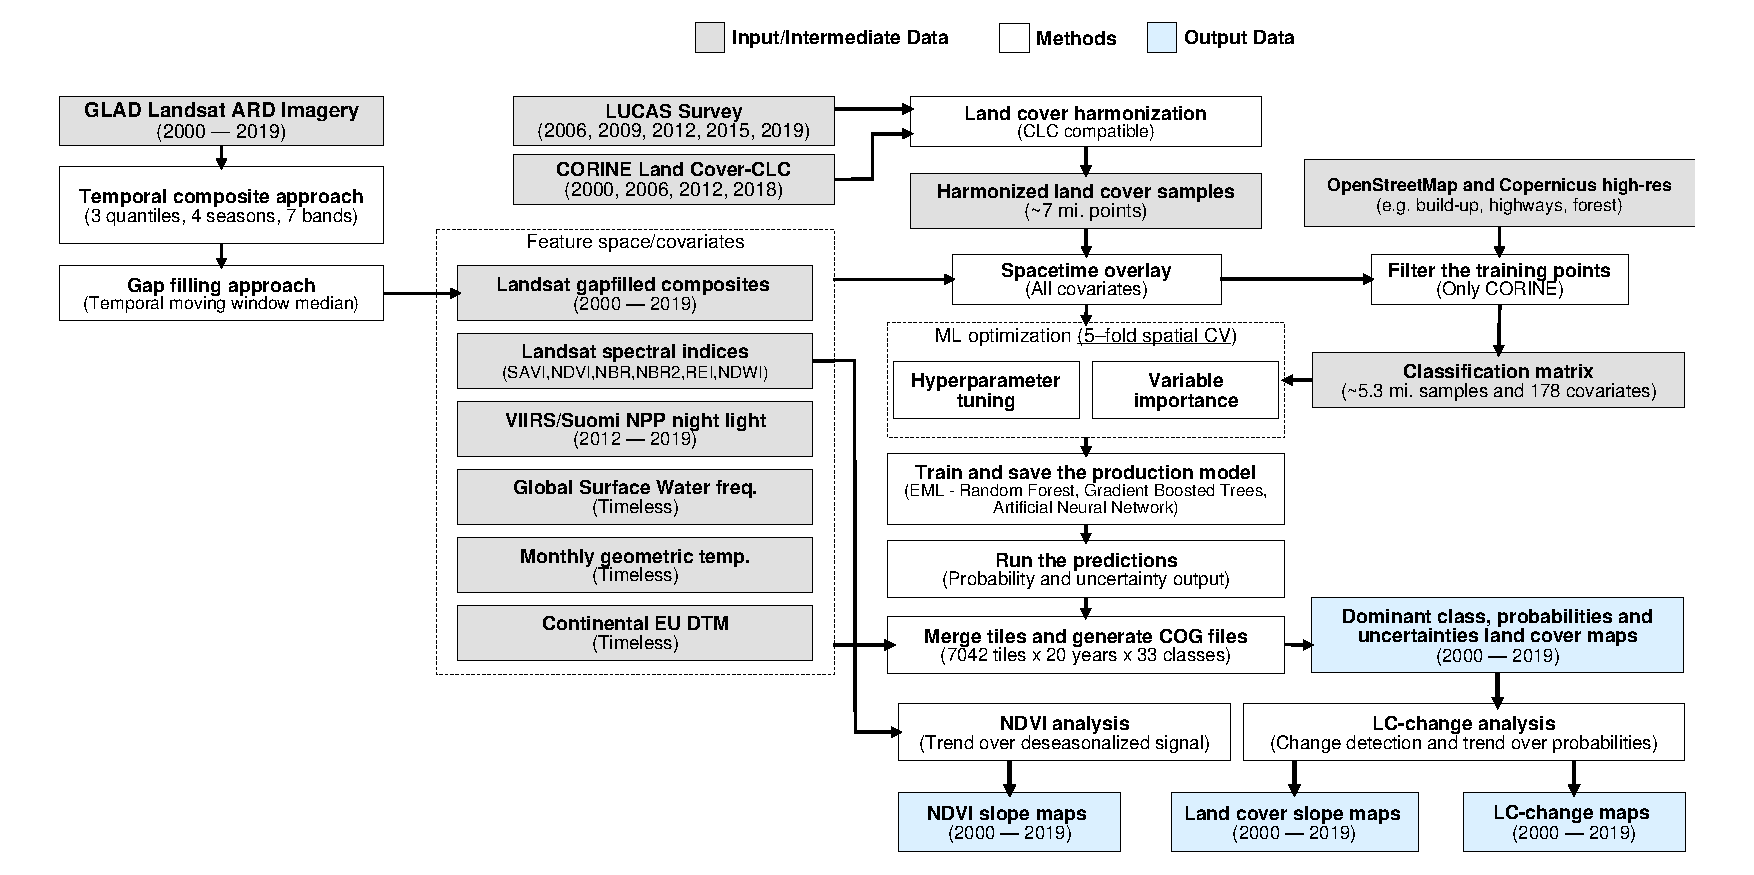
\includegraphics[width=.95\textwidth]{figs_03/methods_general_workflow.pdf}
    \caption{General workflow used to prepare point data and variable layers, fit models and generate annual land cover products (2000--2019). Components of the workflows are described in detail via the \textsf{eumap} library (\url{https://eumap.readthedocs.io/}), with technical documentation available via \url{https://gitlab.com/geoharmonizer_inea/}.} \label{fig:scheme}
    \end{sidewaysfigure}
    
    All the output predictions were predicted first per tile, then exported as Cloud Optimized Geotiffs (COGs) files and are publicly available through the Open Data Science Europe (ODS-Europe) Viewer, the S3 Cloud Object Service, and from \url{http://doi.org/10.5281/zenodo.4725429}. The classification matrix with all training points and variables is available from \url{http://doi.org/10.5281/zenodo.4740691}.
    
\subsection*{Spatiotemporal ensemble modeling}
    
    The annual land cover product for continental Europe was generated with an ensemble of three models and a meta-learner. We used a grid search strategy to find the best hyperparameters and used them to train the final model.
    
        
    Although ensemble training and inference is computationally intensive, it typically achieves higher accuracy than less complex models \citep{seni2010ensemble,zhang2012ensemble}. Furthermore, when each component learner predicts a probability per class, it is possible to use the standard deviation of the per-class probabilities (also known as \emph{model variance}) as an indicator of the prediction uncertainty (see Fig.\@~\ref{fig:ensemble_structure}).

    We selected three component learners among an initial pool of 10 learners based on their performance on sample data:

    \begin{enumerate}
    \item Random Forest \citep{breiman2001random};
    \item Gradient-boosted trees \citep{chen2016xgboost};
    \item Artificial Neural Network \citep{mcculloch1943logical};
    \end{enumerate}

    Each of these models predicts a probability for each class, resulting in 129 probabilities for 43 classes. These component probabilities are forwarded to the meta-learner, a logistic regression classifier \citep{defazio2014saga}, which in turn predicts a single probability per class. The ensemble also outputs the standard deviation of the three component-predicted probabilities per class to generate a class-wise model variance, which can help analyze the data and inform decision-makers where data is more reliable. Because the LUCAS points are based on \emph{in-situ} observations, we considered them as more reliable training data than the CLC centroid points. To prioritize performance on the LUCAS points during model training, we assigned a training weight rating of 100\% to the LUCAS points and 85\% to the CLC points.
    
    \begin{figure}[!hbt]
    \centering
    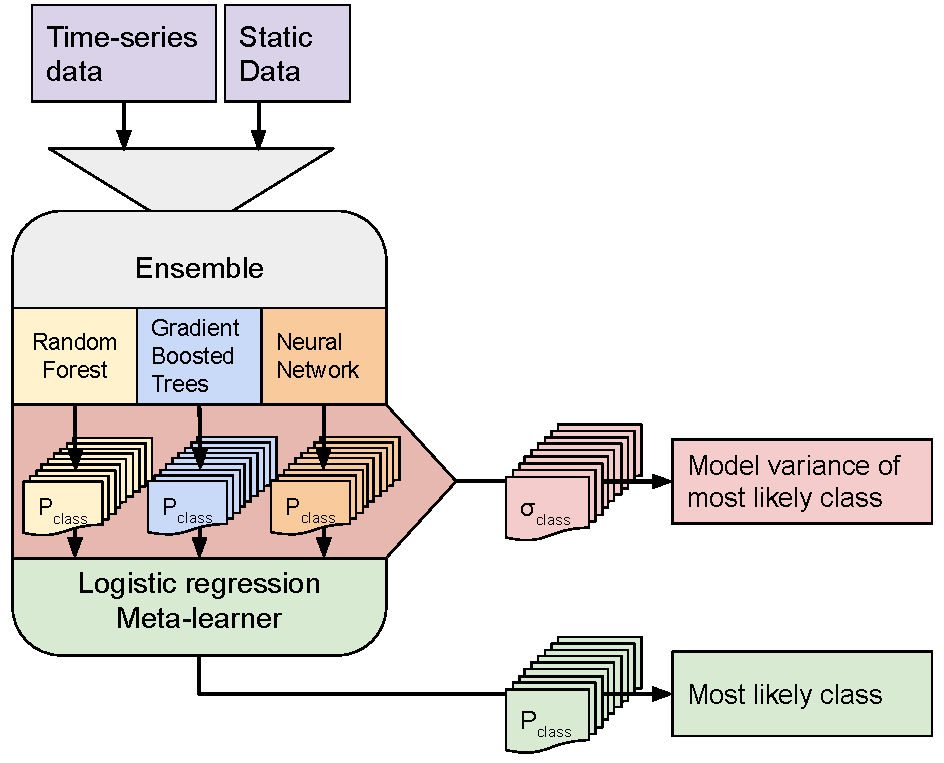
\includegraphics{figs_03/methods_ensemble_structure.pdf}
    \caption{Structure of the ensemble. Time-series data and static data are used to train three component models. Each component model predicts 43 probabilities (1 per class). We calculate class-wise model variance as a proxy of prediction uncertainty as a separate output by taking the standard deviation of the three component probabilities per class. The 129 probabilities are used to train the logistic regression meta-learner, which predicts 43 probabilities that are used to map LULC.}
    \label{fig:ensemble_structure}
    \end{figure}
        
    We optimized the hyperparameters of the random forest and gradient boosted trees component learners by minimizing the logistic (log) loss metric  \citep{lovelace2019geocomputation}:
    \begin{equation}
        L_{\log}(Y, P) = -\log \operatorname{Pr}(Y|P) = - \frac{1}{N} \sum_{i=0}^{N-1} \sum_{k=0}^{K-1} y_{i,k} \log p_{i,k}
    \end{equation}
    
    \noindent where \emph{Y} is a binary matrix of expected class labels, \emph{N} is the total number of observations, \emph{K} is the number of classes, \emph{P} is the matrix of probabilities predicted by the model, \emph{y\textsubscript{i,k}} indicates whether sample \emph{i} belongs to class \emph{k}, and \emph{p\textsubscript{i,k}} indicates the probability of sample \emph{i} belonging to class \emph{j}. A log loss value close to 0 indicate high prediction performance, 0 being a perfect match, while values above 0 indicate progressively worse performance.
    
    We performed 5--fold spatial cross-validation for each different hyperparameter combination (see Table\@~\ref{tab:hyperparameters}. These combinations were generated per model based on a grid search of 5 steps per hyperparameter.
        
    \begin{table}[!hbt]
    \centering
    \caption{Minimum and maximum value of each hyperparameter that was optimized for the random forest and gradient boosted tree learners.}
    \label{tab:hyperparameters}
    \begin{tabular}{@{}llrr@{}}
    \toprule
    Model & Hyperparameter & \multicolumn{1}{l}{Lower value} & \multicolumn{1}{l}{Upper value} \\ 
    \midrule
    Random Forest & Number of estimators & 50 & 100 \\
     & Maximum tree depth & 5 & 50 \\
     & Maximum number of features & 0 & 0.9 \\
     & Minimum samples per leaf & 5 & 30 \\
    Gradient boosted trees & Eta & 0.001 & 0.9 \\
     & Gamma & 0 & 12 \\
     & Alpha & 0 & 1 \\
     & Maximum tree depth & 2 & 10 \\
     & Number of estimators & 10 & 50 \\ 
     \bottomrule
    \end{tabular}
    \end{table}
    
    We evaluated each set of hyperparameters by performing a spatial 5-fold cross-validation. We did this by creating a Europe-wide grid of 30~km tiles (see Fig.\@~\ref{fig:study_area_point_count}) and using the tiles' unique identifiers to group their overlapping points into 5 folds.
    
    After hyperparameter optimization we trained the three component learners on the full dataset. The meta-learner was trained on the probabilities predicted by each component model during the cross-validation of their optimal hyperparameters.

\subsection*{Study area and target classification system}
    
    The study area covers all countries included in the CLC database, except Turkey (see Fig.\@~\ref{fig:study_area_point_count}). The spatiotemporal dataset used in this research contains data from the winter of 1999 to the autumn of 2019.
    
    \begin{figure}[!hbt]
    \centering
    \includegraphics[width=.9\textwidth]{figs_03/methods_study_area_point_count.pdf}
    \caption{Map of the study area, overlaid with a grid of 30~km tiles that was used for spatial 5-fold cross-validation. Grid color indicates the number of training points aggregated per tile.}
    \label{fig:study_area_point_count}
    \end{figure}
    
    The target land cover nomenclature was designed based on CLC nomenclature \citep{bossard2000} and is available in Table\@~\ref{tbl:legend_lc}. CLC is probably the most comprehensive and detailed European land cover product to date. The CLC program was established in 1985 by the European Community to provide geographically harmonized information concerning the environment on the continent. The original CLC dataset is mapped in 44 classes with a minimum mapping unit of 25 ha for areal phenomena and 10 ha for changes. CLC mapping relies on harmonized protocol and guidelines that are shared for country-wise visual photo-interpretation. 
    
    \begin{table}[!hp]
    \centering
    \caption{The  ODSE-LULC land cover legend used based on CLC \citep{bossard2000}. Note: To make table formatting easier, we refer to class 243 as \emph{`Agriculture with significant natural vegetation`} in all other tables.}
    \label{tbl:legend_lc}
    \resizebox{\textwidth}{!}{%
    \begin{tabular}{@{}ll@{}}
    \toprule
    Class name &
      Class description \\ \midrule
    111: Continuous urban fabric &
      \begin{tabular}[c]{@{}l@{}}Surface area covered for more than 80\% by urban structures and other \\ impermeable, artificial features.\end{tabular} \\
    112: Discontinuous urban fabric &
      \begin{tabular}[c]{@{}l@{}}Surface area covered between 30\% and 80\% by urban structures and \\ other impermeable, artificial features.\end{tabular} \\
    121: Industrial or commercial units &
      \begin{tabular}[c]{@{}l@{}}Land units that are under industrial or commercial use or serve for \\ public service facilities.\end{tabular} \\
    122: Road and rail networks &
      Motorways and railways, including associated installations. \\
    123: Port areas &
      Infrastructure of port areas, including quays, dockyards and marinas. \\
    124: Airports &
      Airports installations: runways, buildings and associated land. \\
    131: Mineral extraction sites &
      \begin{tabular}[c]{@{}l@{}}Areas of open-pit extraction of construction materials (sandpits, quarries) \\ or other minerals (open-cast mines).\end{tabular} \\
    132: Dump sites &
      Public, industrial or mine dump sites. \\
    133: Construction sites &
      \begin{tabular}[c]{@{}l@{}}Spaces under construction development, soil or bedrock excavations, \\ earthworks.\end{tabular} \\
    141: Urban green &
      Areas with vegetation within urban fabric. \\
    142: Sport and leisure facilities &
      Areas used for sports, leisure and recreation purposes. \\
    211: Non-irrigated arable land &
      \begin{tabular}[c]{@{}l@{}}Cultivated land parcels under rain-fed agricultural use for annually \\ harvested non-permanent crops, normally under a crop rotation system.\end{tabular} \\
    212: Permanently irrigated arable land &
      \begin{tabular}[c]{@{}l@{}}Cultivated land parcels under agricultural use for arable crops that are \\ permanently or periodically irrigated.\end{tabular} \\
    213: Rice fields &
      \begin{tabular}[c]{@{}l@{}}Cultivated land parcels prepared for rice production, consisting of \\ periodically flooded flat surfaces with irrigation channels.\end{tabular} \\
    221: Vineyards &
      Areas planted with vines. \\
    222: Fruit trees and berry plantations &
      \begin{tabular}[c]{@{}l@{}}Cultivated parcels planted with fruit trees and shrubs, including nuts, \\ intended for fruit production.\end{tabular} \\
    223: Olive groves &
      \begin{tabular}[c]{@{}l@{}}Cultivated areas planted with olive trees, including mixed occurrence \\ of vines on the same parcel.\end{tabular} \\
    231: Pastures &
      \begin{tabular}[c]{@{}l@{}}Meadows with dispersed trees and shrubs occupying up to 50\% of surface \\ characterized by rich floristic composition.\end{tabular} \\
    \begin{tabular}[c]{@{}l@{}}241: Annual crops associated \\ with permanent crops\end{tabular} &
      \begin{tabular}[c]{@{}l@{}}Cultivated land parcels with a mixed coverage of non-permanent (e.g. wheat) and permanent \\ crops (e.g. olive trees).\end{tabular} \\
    242: Complex cultivation patterns &
      \begin{tabular}[c]{@{}l@{}}Mosaic of small cultivated land parcels with different cultivation types \\ (annual and permanent crops, as well as pastures), potentially with scattered houses or gardens.\end{tabular} \\
    \begin{tabular}[c]{@{}l@{}}243: Land principally occupied by \\ agriculture with significant areas of natural vegetation\end{tabular} &
      \begin{tabular}[c]{@{}l@{}}Areas principally occupied with agriculture, interspersed with significant \\ semi-natural areas in a mosaic pattern.\end{tabular} \\
    244: Agro-forestry areas &
      Annual crops or grazing land under the wooded cover of forestry species. \\
    311: Broad-leaved forest &
      \begin{tabular}[c]{@{}l@{}}Vegetation formation composed principally of trees, including shrub and bush understorey, \\ where broad-leaved species predominate.\end{tabular} \\
    312: Coniferous forest &
      \begin{tabular}[c]{@{}l@{}}Vegetation formation composed principally of trees, including shrub and bush understorey,\\ where coniferous species predominate.\end{tabular} \\
    313: Mixed forest &
      \begin{tabular}[c]{@{}l@{}}Vegetation formation composed principally of trees, including shrub and bush understory, \\ where neither broad-leaved nor coniferous species predominate.\end{tabular} \\
    321: Natural grasslands &
      \begin{tabular}[c]{@{}l@{}}Grasslands under no or moderate human influence. Low productivity grasslands. \\ Often in areas of rough, uneven ground, also with rocky areas, or patches of \\ other (semi-)natural vegetation.\end{tabular} \\
    322: Moors and heathland &
      \begin{tabular}[c]{@{}l@{}}Vegetation with low and closed cover, dominated by bushes, shrubs (heather, briars, broom, \\ gorse, laburnum etc.) and herbaceous plants, forming a climax stage of development.\end{tabular} \\
    323: Sclerophyllous vegetation &
      \begin{tabular}[c]{@{}l@{}}Bushy sclerophyllous vegetation in a climax stage of development, \\ including maquis, matorral and garrigue.\end{tabular} \\
    324: Transitional woodland-shrub &
      \begin{tabular}[c]{@{}l@{}}Transitional bushy and herbaceous vegetation with occasional scattered trees. \\ Can represent either woodland degradation or forest regeneration / re-colonization.\end{tabular} \\
    331: Beaches, dunes, sands &
      \begin{tabular}[c]{@{}l@{}}Natural un-vegetated expanses of sand or pebble/gravel, in coastal or continental locations, \\ like beaches, dunes, gravel pads.\end{tabular} \\
    332: Bare rocks &
      Scree, cliffs, rock outcrops, including areas of active erosion. \\
    333: Sparsely vegetated areas &
      Areas with sparse vegetation, covering 10-50\% of the surface. \\
    334: Burnt areas &
      Areas affected by recent fires. \\
    335: Glaciers and perpetual snow &
      Land covered by ice or permanent snowfields. \\
    411 Inland marshes &
      \begin{tabular}[c]{@{}l@{}}Low-lying land usually flooded in winter, and with ground more or less \\ saturated by fresh water all year round.\end{tabular} \\
    412 Peat bogs &
      \begin{tabular}[c]{@{}l@{}}Wetlands with accumulation of considerable amount of decomposed moss (mostly Sphagnum) \\ and vegetation matter. Both natural and exploited peat bogs.\end{tabular} \\
    421 Salt marshes &
      \begin{tabular}[c]{@{}l@{}}Vegetated low-lying areas in the coastal zone, above the high-tide line, \\ susceptible to flooding by seawater.\end{tabular} \\
    422 Salines &
      \begin{tabular}[c]{@{}l@{}}Sections of salt marsh exploited for the production of salt by evaporation, active or in process \\ of abandonment, distinguishable from marsh by parcellation or embankment systems.\end{tabular} \\
    423 Intertidal flats &
      \begin{tabular}[c]{@{}l@{}}Area between the average lowest and highest sea water level at low tide and high tide. Generally \\ non-vegetated expanses of mud, sand or rock lying between high and low water marks.\end{tabular} \\
    511: Water courses &
      Natural or artificial water courses for water drainage channels. \\
    512: Water bodies &
      Natural or artificial water surfaces covered by standing water most of the year. \\
    521: Coastal lagoons &
      \begin{tabular}[c]{@{}l@{}}Stretches of salt or brackish water in coastal areas which are separated from the sea \\ by a tongue of land or other similar topography.\end{tabular} \\
    522: Estuaries &
      The mouth of a river under tidal influence within which the tide ebbs and flows. \\ \bottomrule
    \end{tabular}%
    }
    \end{table}
    
    The  ODSE-LULC nomenclature is identical to the CLC legend, excluding class 523: Sea and ocean, as we omitted such areas from our study area to reduce computation time. The CLC classification system has been reported to be unsuitable for pixel-wise classification due to the inclusion of: 1) heterogeneous and mixed classes defined for polygon mapping (e.g. airports, road and rail networks, complex cultivation patterns, agro-forestry, etc.) and 2) classes primarily distinguishable by land use, not land cover (e.g. commercial and industrial units, sports and leisure facilities). We did not remove these classes beforehand to provide objective information about the performance of the CLC level 3 legend for pixel-wise classification, and to enable a complete comparison to the S2GLC nomenclature, which is more optimized for such pixel-based classification.

\subsection*{Training points}

    We obtained the training dataset from the geographic location of LUCAS (\emph{in-situ} source) and the centroid of all CLC polygons (as shown in Fig.\@~\ref{fig:tp_workflow}), harmonized according to the 43 land cover classes (see Table\@~\ref{tbl:legend_lc}) and organized by year, where each unique combination of longitude, latitude and year was considered as an independent sample, resulting in more than 8~million training points.
    
    
    
    The LUCAS data from 2006, 2009, 2012, 2015 and 2018, as provided by Eurostat (obtained from: \url{https://ec.europa.eu/eurostat/web/lucas}) is the largest and most comprehensive \emph{in-situ} land cover dataset for Europe. The survey has evolved since 2000 and requires harmonisation before it can be used for mapping over several years. We imported datasets from individual years and harmonized these before merging it into one common database with an automated workflow implemented in Python and SQL (Fig.\@~\ref{fig:scheme}). For the multi-year harmonization procedure we first harmonized attribute names, re-coded variables, harmonized point locations, and aggregated the points based on their location in space and time. After these operations, we translated the LUCAS land cover nomenclature to the  ODSE-LULC nomenclature, Table\@~\ref{tbl:legend_lc}, according to the method designed by \citet{buck}. The distribution of all reference points per CLC class and per survey year is shown in Fig.\@~\ref{fig:dataset_countplot}.
    
    
    
    \begin{figure}[!hp]
    \centering
    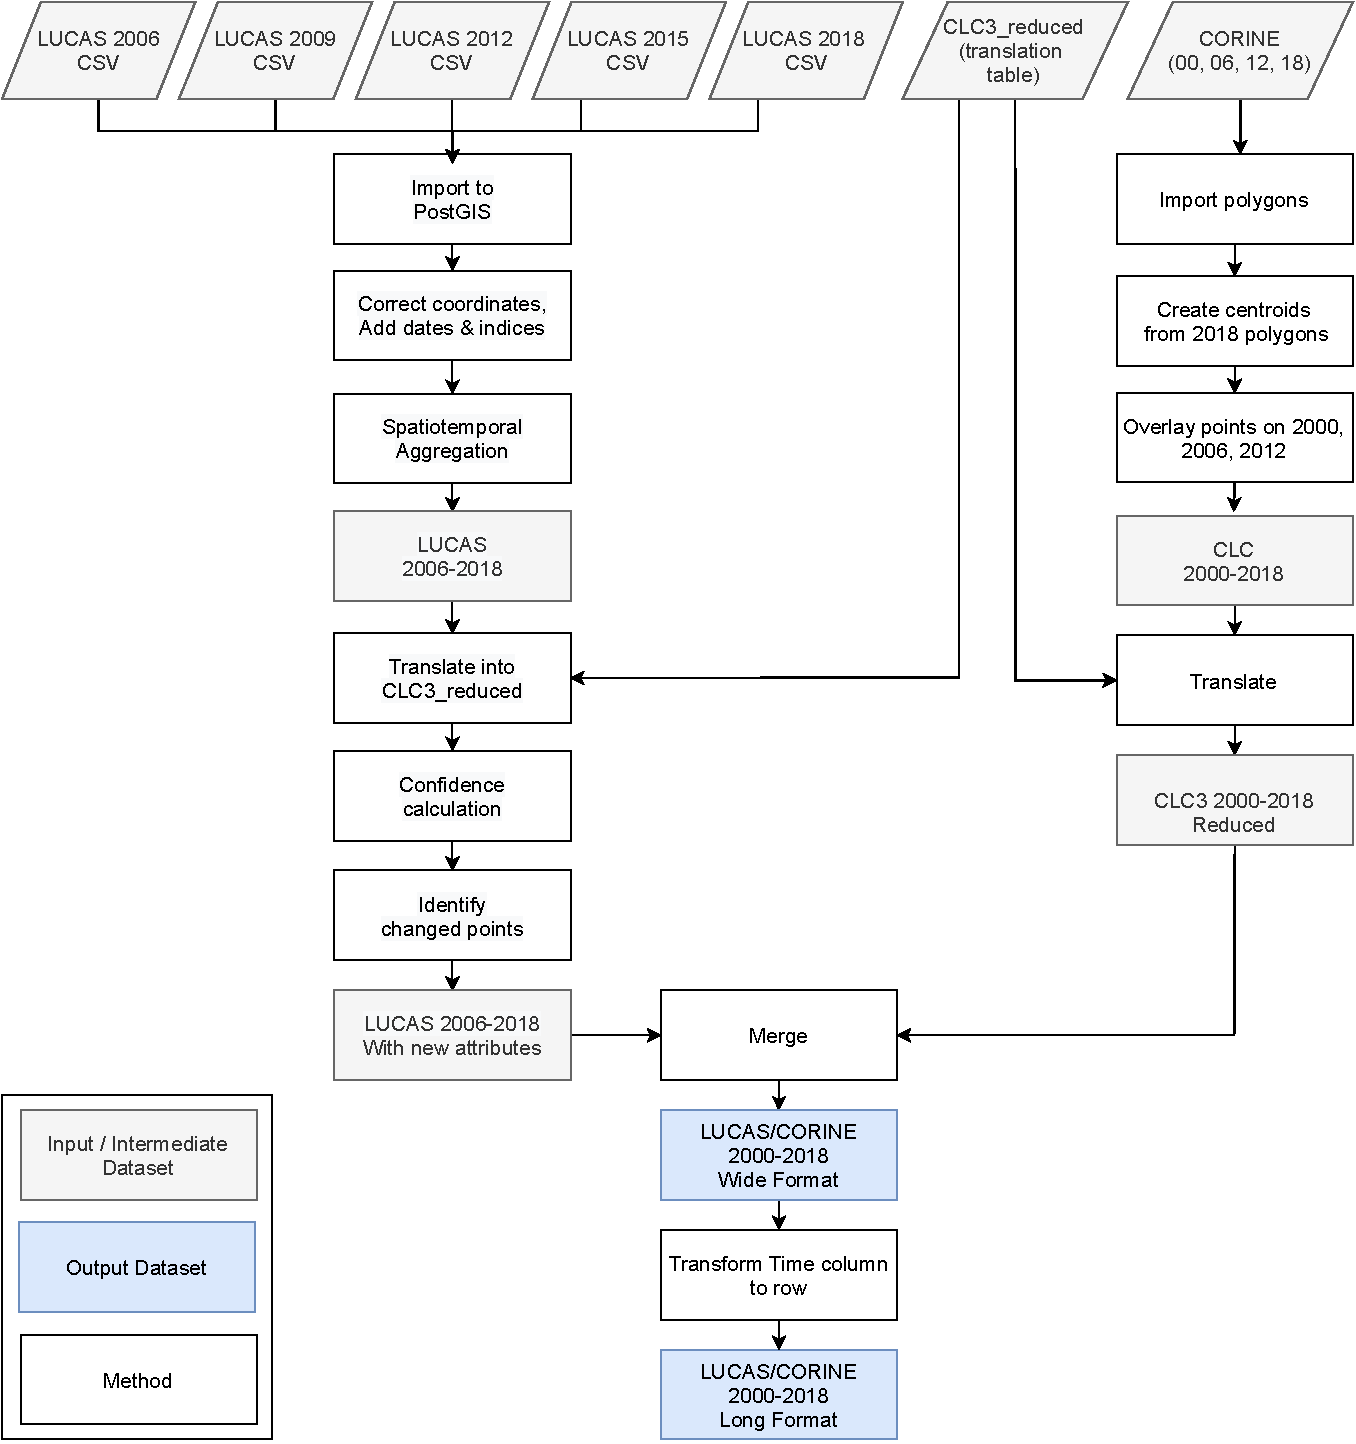
\includegraphics[width=\textwidth]{figs_03/methods_lucas_corine_workflow.pdf}
    \caption{General workflow for merging training points obtained from LUCAS and CLC.} \label{fig:tp_workflow}
    \end{figure}
    
    \begin{figure}[!hp]
    \centering
    % \vspace*{-1.5cm}
        % \hspace*{-3.5cm}
        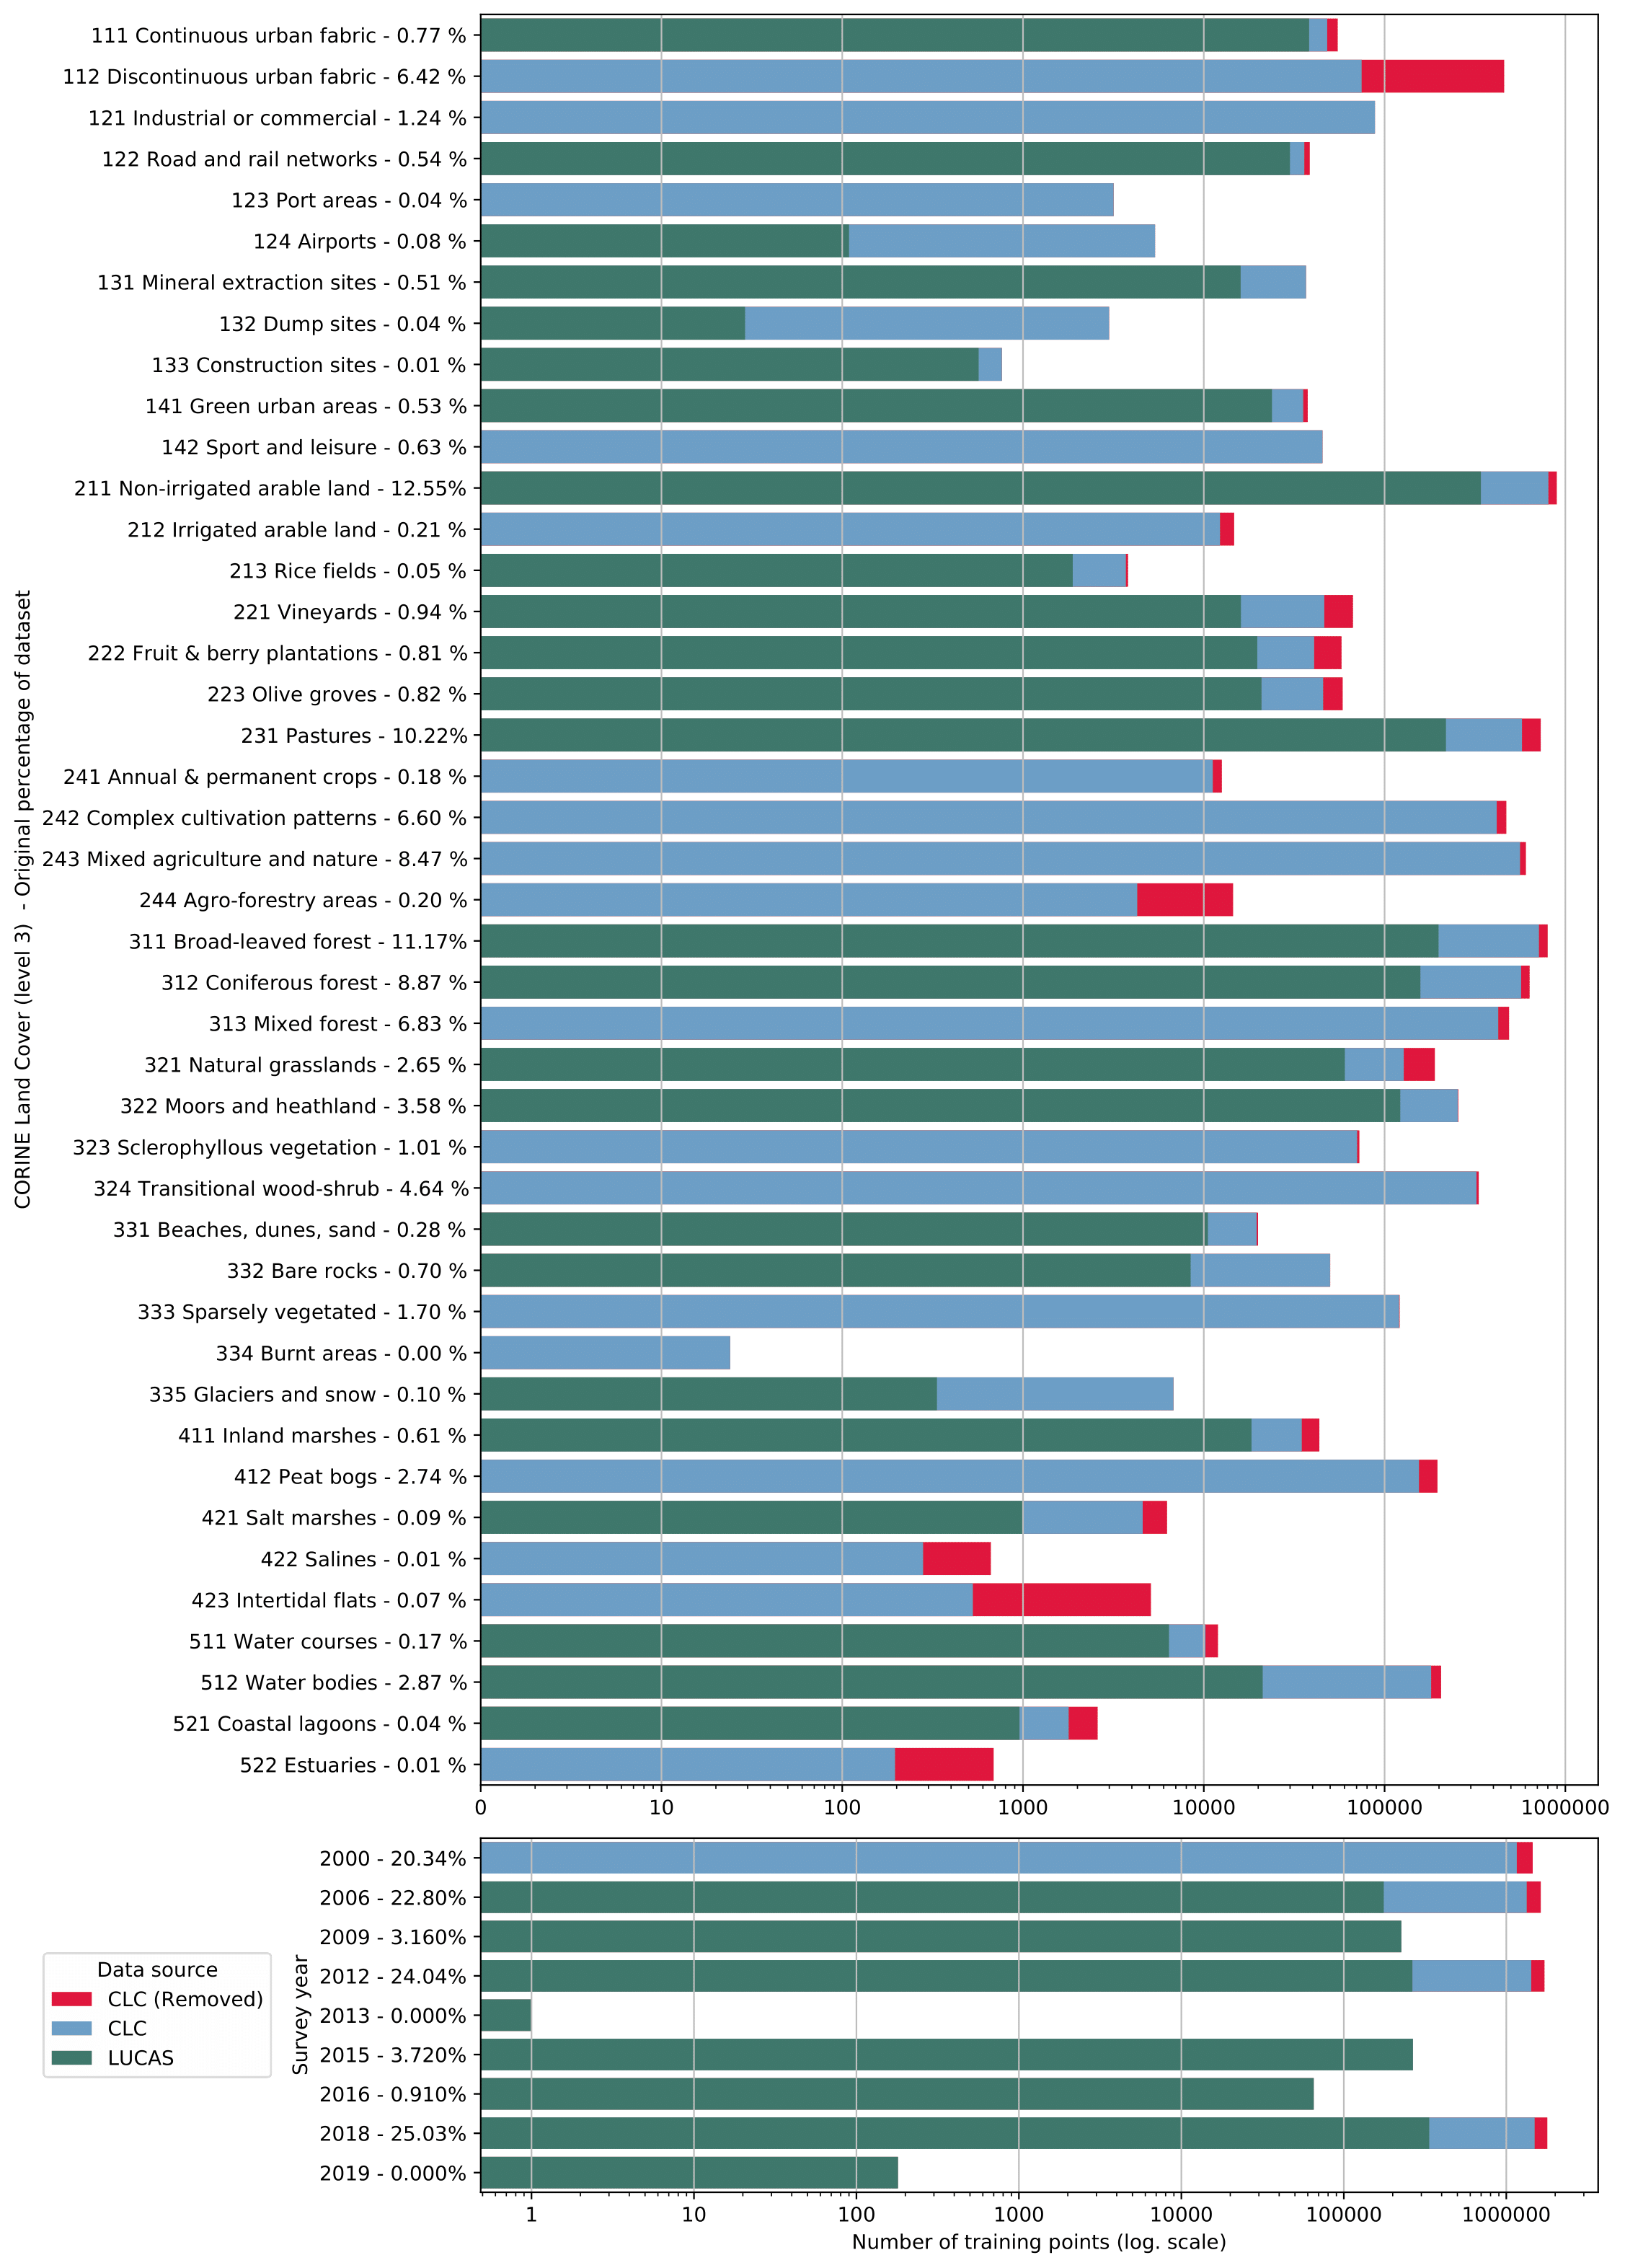
\includegraphics[width=1\textwidth]{figs_03/methods_dataset_countplot.png}
    \caption{Distribution of training points per data source (blue and green), class (top) and per survey year (bottom). The proportion of removed CLC points is indicated in red.}
    \label{fig:dataset_countplot}
    \end{figure}
    

    The CLC minimal mapping unit of 25~ha required filtering on the training points before they could be used to represent 30~m resolution LULC, for example, to remove points for \emph{``111: urban fabric''} located in small patches of urban greenery ($<$25~ha). For this purpose, we extracted vector data from OSM layers for roads, railways, and buildings (obtained from \url{https://download.geofabrik.de/}). We then created a 30~m density raster for each feature type. This was done by first creating a 10~m raster where each pixel intersecting a vector feature was assigned the value 100. These pixels were then aggregated to 10~m resolution by calculating the average of every 9 adjacent pixels.
    This resulted in a 0\textemdash100 density layer for the three feature types. 
    Although the digitized building data from OSM offers the highest level of detail, its coverage across Europe is inconsistent. To supplement the building density raster in regions where crowd-sourced OSM building data was unavailable, we combined it with Copernicus High Resolution Layers (HRL) (obtained from \url{https://land.copernicus.eu/pan-european/high-resolution-layers}), filling  the non-mapped areas in OSM with the Impervious Built-up 2018 pixel values, which was averaged to 30~m. The probability values produced by the averaged aggregation were integrated in such a way that values between 0\textemdash100 refer to OSM (lowest and highest probabilities equal to 0 and 100 respectively), and the values between 101\textemdash200 refer to Copernicus HRL (lowest and highest probability equal to 200 and 101 respectively). This resulted in a raster layer where values closer to 100 are more likely to be buildings than values closer to 0 and 200. Structuring the data in this way allows us to select the higher probability building pixels in both products by the single boolean expression: pixel \textgreater{} 50 AND pixel \textless 150.
    
    We also use HRL products to filter other classes: Table\@~\ref{tab:filter_rules} shows the exact conditions points of specific LULC classes needed to meet in order to be retained in our dataset. This procedure is similar to the one used by \citet{inglada2017operational}. This filtering process removed about 1.3 million points from our training dataset, resulting in a classification matrix with a total of ca.\@ 8.1~million samples and 232 variables. The classification matrix used to produce  ODSE-LULC is available from \url{http://doi.org/10.5281/zenodo.4740691}.
    
    \begin{table}[!hbt]
    \centering
    \caption{Per-class conditions applied only to CLC points during the filtering step. All the raster layers were upsampled to 30\texttimes30~m resolution by average and the points that did not meet the specified condition were omitted from the training dataset.}
    \label{tab:filter_rules}
    
    \resizebox{\textwidth}{!}{%
    \begin{tabular}{@{}lll|llllll|lll@{}}
    \toprule
     &  & Condition & HRL & & &  &  &  & OSM &  & HRL+OSM \\
    Code & Class &  & \begin{tabular}[c]{@{}l@{}}Tree \\ Cover\end{tabular} & Grass & Imp. & \begin{tabular}[c]{@{}l@{}}Perm. \\ Water\end{tabular} & \begin{tabular}[c]{@{}l@{}}Perm. \\ Wetness\end{tabular} & \begin{tabular}[c]{@{}l@{}}Temp. \\ Wetness\end{tabular} & Rails & Roads & Buildings \\ \midrule
    111 & Continuous urban fabric & - &  &  &  &  &  &  &  &  & \textgreater{}50 and \textless 150 \\
    112 & Discontinuous urban fabric &  &  &  &  &  &  &  &  &  & \textgreater{}50 and \textless 150 \\
    121 & Industrial or commercial units &  &  &  &  &  &  &  &  &  &  \\
    122 & Road and rail networks and associated land & OR &  &  & \textgreater{}30 &  &  &  & \textgreater{}30 & \textgreater{}30 &  \\
    123 & Port areas &  &  &  &  &  &  &  &  &  &  \\
    124 & Airports &  &  &  &  &  &  &  &  &  &  \\
    131 & Mineral extraction sites & AND & = 0 & = 0 &  &  &  &  &  &  &  \\
    132 & Dump sites &  &  &  &  &  &  &  &  &  &  \\
    133 & Construction sites &  &  &  &  &  &  &  &  &  &  \\
    141 & Green urban areas & ( OR ) AND & \textgreater{}0 & \textgreater{}0 &  &  &  &  &  &  & \textless{}50 or \textgreater 150 \\
    142 & Sport and leisure facilities &  &  &  &  &  &  &  &  &  &  \\
    211 & Non-irrigated arable land & AND & = 0 &  &  &  &  &  & = 0 & = 0 & \textless{}50 or \textgreater 150 \\
    212 & Permanently irrigated arable land &  & = 0 &  &  &  &  &  & = 0 & = 0 & \textless{}50 or \textgreater 150 \\
    213 & Rice fields &  &  &  &  &  &  &  & = 0 & = 0 & \textless{}50 or \textgreater 150 \\
    221 & Vineyards & AND &  & = 0 &  &  &  &  & = 0 & = 0 & \textless{}50 or \textgreater 150 \\
    222 & Fruit trees and berry plantations & AND &  & = 0 &  &  &  &  & = 0 & = 0 & \textless{}50 or \textgreater 150 \\
    223 & Olive groves & AND &  & = 0 &  &  &  &  & = 0 & = 0 & \textless{}50 or \textgreater 150 \\
    231 & Pastures & AND & = 0 &  &  &  &  &  & = 0 & = 0 & \textless{}50 or \textgreater 150 \\
    241 & Annual crops associated with permanent crops &  &  &  &  &  &  &  & = 0 & = 0 & \textless{}50 or \textgreater 150 \\
    242 & Complex cultivation patter &  &  &  &  &  &  &  & = 0 & = 0 & \textless{}50 or \textgreater 150 \\
    243 & Agriculture with significant natural vegetation &  &  &  &  &  &  &  & = 0 & = 0 & \textless{}50 or \textgreater 150 \\
    244 & Agro-forestry areas &  & \textgreater{}0 &  &  &  &  &  & = 0 & = 0 & \textless{}50 or \textgreater 150 \\
    311 & Broad-leaved forest & AND & \textgreater{}0 &  &  &  &  &  & = 0 & = 0 & \textless{}50 or \textgreater 150 \\
    312 & Coniferous forest & AND & \textgreater{}0 &  &  &  &  &  & = 0 & = 0 & \textless{}50 or \textgreater 150 \\
    313 & Mixed forest &  & \textgreater{}0 &  &  &  &  &  & = 0 & = 0 & \textless{}50 or \textgreater 150 \\
    321 & Natural grasslands & AND & = 0 & \textgreater{}0 &  &  &  &  & = 0 & = 0 & \textless{}50 or \textgreater 150 \\
    322 & Moors and heathland &  &  &  &  &  &  &  & = 0 & = 0 & \textless{}50 or \textgreater 150 \\
    323 & Sclerophyllous vegetation &  &  &  &  &  &  &  & = 0 & = 0 & \textless{}50 or \textgreater 150 \\
    324 & Transitional woodland-shrub &  &  &  &  &  &  &  & = 0 & = 0 & \textless{}50 or \textgreater 150 \\
    331 & Beaches, dunes, sand &  &  &  &  &  &  &  & = 0 & = 0 & \textless{}50 or \textgreater 150 \\
    332 & Bare rocks &  &  &  &  &  &  &  & = 0 & = 0 & \textless{}50 or \textgreater 150 \\
    333 & Sparsely vegetated areas &  &  &  &  &  &  &  & = 0 & = 0 & \textless{}50 or \textgreater 150 \\
    334 & Burnt areas &  &  &  &  &  &  &  & = 0 & = 0 & \textless{}50 or \textgreater 150 \\
    335 & Glaciers and perpetual snow &  &  &  &  &  &  &  & = 0 & = 0 & \textless{}50 or \textgreater 150 \\
    411 & Inland marshes & OR &  &  &  &  & \textgreater{}0 & \textgreater{}0 & = 0 & = 0 & \textless{}50 or \textgreater 150 \\
    412 & Peat bogs &  &  &  &  &  &  &  & = 0 & = 0 & \textless{}50 or \textgreater 150 \\
    421 & Salt marshes &  &  &  &  &  &  &  & = 0 & = 0 & \textless{}50 or \textgreater 150 \\
    422 & Salines &  &  &  &  &  &  &  & = 0 & = 0 & \textless{}50 or \textgreater 150 \\
    423 & Intertidal flats &  &  &  &  &  &  &  & = 0 & = 0 & \textless{}50 or \textgreater 150 \\
    511 & Water courses &  &  &  &  & \textgreater{}50 &  &  &  &  &  \\
    512 & Water bodies & - &  &  &  & = 100 &  &  &  &  &  \\
    521 & Coastal lagoons &  &  &  &  & \textgreater{}50 &  &  &  &  &  \\
    522 & Estuaries &  &  &  &  & \textgreater{}50 &  &  &  &  &  \\ \bottomrule
    \end{tabular}%
    }
    \end{table}

    We assessed the quality of the training dataset by comparing it to a number of existing land cover products:
        
    \begin{itemize}
    \item GLFCS30--2015 \citep{zhang2020glcfcs30};
    \item GLFCS30--2020 \citep{zhang2020glcfcs30};
    \item S2GLC \citep{malinowski2020};
    \item The European land cover product for 2015 created by \citet{pflugmacher2019mapping};
    \item  ELC10 \citep{venter2021continentalscale}.
    \end{itemize}
    
    For each comparison, we reclassified the training dataset to the nomenclature of the target dataset and overlaid all points from our dataset with survey dates from within one year of the land cover product. We then calculated the weighted F1-score as if the points represented predictions. Points with classes of the target products that were completely absent in the training point subsets (due to the target nomenclature of the training points) were removed before these assessments, potentially resulting in varying numbers of classes for the same dataset. 
    
    The GLFCS30 nomenclature was not suitable for direct translation because some land cover types (such as forests) are separated into several subcategories. We therefore aggregated their thematic resolution to the higher level of abstraction described in \citet{zhang2020glcfcs30}. The complete translation scheme is available via the GitLab repository of the GeoHarmonizer project (\url{https://gitlab.com/geoharmonizer_inea/spatial-layers}).

\subsection*{Input variables}
    
    In this work we combine harmonized time-series data of varying temporal resolution with static datasets. The time-series data consists of the following:
    
    \begin{itemize}
    \item Seasonal aggregates of Landsat spectral bands (blue, green, red, NIR, SWIR1, SWIR2, thermal), divided into 3 reflectance quantiles per and 4 seasons, resulting in 12 layers per band;
    \item Spectral indices calculated from the seasonal Landsat data: NDVI, SAVI, MSAVI, NDMI, Landsat NBR, REI, and NDWI derived according to formulas in Table\@~\ref{tab:spectral_indices};
    \item Terrain Roughness Index (TRI) of the Landsat green band (50th reflectance quantile of summer);
    \item SUOMI NPP VIIRS night light imagery downscaled from 500~m to 30~m resolution \citep{hillger2013first};
    \item Monthly geometric minimum and maximum temperature \citep{kilibarda2014spatio};
    \end{itemize}
    
    Additional static datasets are:
    
    \begin{itemize}
    \item Probability of surface water occurrence at 30~m resolution \citep{pekel2016high};
    \item Continental EU DTM-based elevation and slope in percent \citep{hengl2020dtm};
    \end{itemize}

    All variables used by our model are derived from remotely sensed EO data from multiple sources, the largest share being derived from Landsat imagery. Although EO data with higher spatial and temporal resolution, as well as actual surface reflection values are available (e.g. Sentinel-2), such sources do not cover the timespan required for the long-term analysis proposed by this framework. The Landsat data used in this work was obtained by downloading the Landsat ARD, provided by GLAD \citep{potapov2020landsat}, for the years 1999 to 2019 and for the entire extent of continental Europe (see \textsf{eumap} landmask \citep{hengl2020dtm}). This imagery archive was screened to remove the cloud and cloud shadow pixels, maintaining only the quality assessment-QA values labeled as clear-sky according to GLAD. Second, we averaged the individual images by season according to three different quantiles (25th, 50th and 75th) and the following calendar dates for all periods:
    
    \begin{itemize}
    \item Winter: December 2 of previous year until March 20 of current year;
    \item Spring: March 21 until June 24 of current year;
    \item Summer: June 25 until September 12 of current year;
    \item Fall: September 13 until December 1 of current year.
    \end{itemize}
    
    We decided to use the equal length definition provided by \citet{trenberth1983seasons} representing four seasons and matching the beginning and end of each season with the 16-day intervals used by \citet{potapov2020landsat}. From more than 73~TB of input data we produced 84 images (3 quantiles $\times$ 4 seasons $\times$ 7 Landsat bands) for each year with different occurrences of no-data values due to cloud contamination in all observations of a specific season. 
    
    We next impute all missing values in the Landsat temporal composites using the \emph{``Temporal Moving Window Median''} (TMWM) algorithm, implemented in python and publicly available in the \textsf{eumap} library (see Fig.\@~\ref{fig:scheme}). The algorithm uses the median values derived from temporal neighbours to impute a missing value using pixels from 1)\@~the same season, 2)\@~neighboring seasons and 3\@~the full year. For example, for a missing value in the spring season, the algorithm first tries to use values from spring seasons of neighbouring years. If no pixel value is available for the entire period (i.e. 2000--2019), the algorithm tries to use values from winter and summer of neighbouring years. If no pixel value is available from data of adjacent seasons from the same year, pixel values from adjacent years are used to derive the median values. Ultimately, a missing value will not receive an impute value only if the pixel lacks data throughout the entire time-series. The median calculation considers different sizes of temporal windows, which expands progressively for each impute attempt (i.e. \texttt{time\_win\_size} parameter); in this work we used a maximum \texttt{time\_win\_size} of 7. We selected the TMWM approach from a set of 4 algorithms through a benchmarking process. To our knowledge, it provides the best combination of gap-filling accuracy and computational costs on the scale of this project.

    We include several spectral indices as a form of feature engineering because they are each designed and tested to help identify or distinguish different types of land cover.  Table\@~\ref{tab:spectral_indices} provides an overview of how we derived them from the Landsat data. This was done for each quantile and each season, resulting in 4~{\texttimes}~3~=~12 variables per spectral index.
    
    \renewcommand{\arraystretch}{1.8}
    \begin{center}
    \small
    % \begin{table}
    \captionof{table}{Spectral indices derived from the Landsat data and used as additional variables in the spatiotemporal EML.}
    \begin{tabular}{ccc}
    \label{tab:spectral_indices}
    Spectral Index & Equation & Reference\\
    \hline
    NDVI &
    $\begin{aligned} % placement: default is "center", options are "top" and "bottom"
    \frac{nir - red}{nir + red}
    \end{aligned}$ & \citep{tucker1979red}\\
    SAVI &
    $\begin{aligned} % placement: default is "center", options are "top" and "bottom"
    \frac{nir - red}{(nir + red + 0.5) \times 1.5)}
    \end{aligned}$ & \citep{huete1988savi}\\
    MSAVI &
    $\begin{aligned} % placement: default is "center", options are "top" and "bottom"
    \frac{(2 \times nir + 1) - \sqrt{(2 \times nir + 1)^{2} - 8 \times (nir - red)}}{2}
    \end{aligned}$ &  \citep{qi1994msavi}\\
    NDWI &
    $\begin{aligned} % placement: default is "center", options are "top" and "bottom"
    \frac{green - swir2}{green + swir2}
    \end{aligned}$ & \citep{gao1996ndwi}\\
    NBR &
    $\begin{aligned} % placement: default is "center", options are "top" and "bottom"
    \frac{nir - thermal}{nir + thermal}
    \end{aligned}$ & \citep{key1999nbr}\\
    NDMI &
    $\begin{aligned} % placement: default is "center", options are "top" and "bottom"
    \frac{nir - swir1}{nir + swir1}
    \end{aligned}$ & \citep{jin2005ndmi}\\
    NBR2 &
    $\begin{aligned} % placement: default is "center", options are "top" and "bottom"
    \frac{swir1 - thermal}{swir1 + thermal}
    \end{aligned}$ & \citep{key2006nbr2}\\
    REI &
    $\begin{aligned}
    {\frac{nir - blue}{nir + blue}}\times{nir}
    \end{aligned}$ & \citep{shahi2015novel}
    \end{tabular}
    % \end{table}
    \end{center}
    \renewcommand{\arraystretch}{1}
    
    The TRI \citep{riley1999index} gives an indication of how different pixel values are from those of its neighbors. Is usually calculated from elevation data, but we include it as a derivative of the Landsat green band in order to help the model distinguish between pixels that are part of larger, homogeneous regions from pixels that are located inside more heterogeneous landscapes (e.g. airports, urban green areas, and forest edges).
        
    The Suomi-NPP VIIRS night light imagery \citep{hillger2013first} was included to introduce a variable that may help the model recognize the built-up environment, but also distinguish different types of land use within that category. This data is originally in 500~m resolution, but we re-sampled them to 30~m using a cubic spline.
    
    The geometric minimum and maximum temperature is a geometric transformation of latitude and the day of the year \citep{kilibarda2014spatio}. We include these variables to improve performance on LULC classes that occur in different situations under distant latitudes e.g.\@ coniferous forest in Greece and Norway. It can be defined anywhere on the globe using Eq.(\ref{tgeom}):
        
    \begin{align}
    \label{tgeom}
    t_{min} &= 24.2 \cdot \cos\phi -15.7 \cdot (1-\cos\theta) \cdot \sin|\phi| - 0.6 \cdot \frac{z}{100}  \\
    t_{max} &= 37 \cdot \cos\phi -15.4 \cdot (1-\cos\theta) \cdot \sin|\phi| - 0.6 \cdot \frac{z}{100}
    \end{align}
    
    \noindent where $\theta$ is derived as:
    
    \begin{equation}
    \label{eq:teta}
    \theta = (day-18) \cdot \frac{2\pi}{365} + 2^{1-\mathrm{sgn}(\phi)} \cdot \pi.
    \end{equation}
    
    \noindent where $day$ is the day of year, $\phi$ is the latitude, the number 18 represents the coldest day in the northern and warmest day in the southern hemisphere, $z$ is the elevation in meter, 0.6 is the vertical temperature gradient per 100~m, and $\mathrm{sgn}$ denotes the signum function that extracts the sign of a real number. 
        
    We include a long-term (35-year) probability estimate of surface water occurrence \citep{pekel2016high} based on the expectation that it would improve model performance when classifying LULC classes associated with water, such as wetlands and rice fields.

\subsection*{Accuracy assessment}
    We evaluate the suitability of the proposed framework with three assessments:
    \begin{enumerate}
        \item Comparison of spatial and spatiotemporal models;
        \item 5-fold spatial cross-validation;
        \item Validation on S2GLC point data.
    \end{enumerate}
    
    we compare the performance of spatial and spatiotemporal models to assess whether training models on data from multiple years can improve their ability to generalize to data from unknown years. We expect models trained on observations from multiple years to generalize better on data from unknown years than models trained on observations from a single year. In order to investigate this, we trained multiple ensemble models on several subsets of our training data that were selected from either one or several years, and validated them on data from years included in their training data and on observations from 2018, the last year of the training dataset, upon which no model was trained.
    
    The validation on the S2GLC point data is included to assess the extent to which the choice of legend affects the classification accuracy of our framework. The S2GLC legend contains less classes and does not 

    The results produced by the 5-fold spatial cross-validation are used to assess four characteristics of the proposed methodology:
    \begin{enumerate}
        \item The difference in performance between the ensemble model and its component models;
        \item classification accuracy of the framework when reproducing the 43-class CLC classification system;
        \item consistency of prediction accuracy by the framework through time;
        \item consistency of prediction accuracy by the framework through space;
    \end{enumerate}
    
    In all comparisons and experiments, we discriminate model performance with the Weighted F1-score metric \citep{van1980information}:
    
    \begin{equation}
        \mathrm{WF}_1 = \sum_{c=1}^{n}{S_{c} \cdot \frac{2 \cdot P_{c} \cdot R_{c}}{P_{c} + R_{c}}}
    \end{equation}
    
    \noindent where $n$ is the number of classes, and $S_{c}$ is the support (the number of training points), $P_{c}$ the precision (producer's accuracy), and $R_{c}$ the recall (user's accuracy) of a given class $c$. We used a weighted version of this metric because it distinguishes classification performance more strictly on imbalanced datasets, such as the one used in this work.
    
    
    
    \subsubsection*{Spatial Cross-validation}
        
        Before mapping LULC in continental Europe for all years, we performed spatial 5-fold cross-validation using the hyperparameters of the final EML model to assess its performance. The predictions for the points from each left-out fold were merged into one set of predicted values, which we used to assess the performance of our final model.
        We did this for each of the three levels in the CLC nomenclature (with 43, 15, and 5 classes) to investigate the effect of legend size. We aggregated predictions to the higher level in the hierarchy by taking the highest probability among subclasses within the same higher level class before selecting the most probable class. Besides this general performance on the total dataset, we also analyzed the performance of the ensemble per class, year, and cross-validation tile.
        
        Analyzing the performance per class and per level in the hierarchy allows us to quantify the performance increase gained from aggregating specific classes. We do this by calculating the weighted average of the F1-score of all sub-classes of a higher-level class (e.g. 311: Broad-leaved forest, 312: Coniferous forest, and 313: Mixed forest, which together comprise the level 2 class 31: Forests and seminatural areas). Finally, we subtract the weighted average F1-score of the subclasses from the F1-score of the higher-level class to quantify the performance gain. This value will tend to be higher when the model frequently confuses sub-classes of a higher-level class, as aggregation then removes more classification errors.
        
        We analyzed the temporal and spatial consistency of our model performance by calculating the weighted F1-scores for the cross-validation predictions on points from each separate year and tile, respectively. We calculated the standard deviation of these scores to assess the consistency of the model. 
        
        Finally, we also compare the cross validation log loss score per class, as well as aggregated per CLC level, with a baseline log loss score. This baseline log loss is what a random classifier would score when predicting on a given dataset. A dataset with more classes and a more unequal distribution has a higher baseline log loss score. We also calculate a log loss ratio to give a measure of model performance that is agnostic of the number and distribution of classes, instead only reflecting how well a given model performed given the difficulty of its task. We define this ratio as follows:
        
        \begin{equation}
            R(Y,P) = 1-\frac{L_{\log}(Y, P)}{B_{\log}(Y, P)}
        \end{equation}
        
        \noindent where \emph{L\textsubscript{log}} indicates the log loss score of the prediction and \emph{B\textsubscript{log}} indicates the baseline log loss score that would be scored by a randomly predicting model. A ratio of 0 means that the model did not outperform a random predictor, a ratio of 1 means a perfect prediction with a log loss score of 0.
    
    \subsubsection*{Validation on S2GLC points}
        
        After training an ensemble model with the same hyperparameters on all training data, we classified LULC in 2017. This prediction was validated with the S2GLC dataset which \citet{malinowski2020} used to validate their 2017 land cover product. The dataset contains 51,926 points with human-verified land cover classifications which were collected with a stratified random sampling method from 55 proportionally selected regions of Europe.
        
        As the S2GLC points follow a different nomenclature, we translated the  ODSE-LULC predicted classes according to Table\@~\ref{tab:malinowski_keys}. Because any predicted classes outside the S2GLC nomenclature (labeled as 000: None in Table\@~\ref{tab:malinowski_keys}) would be automatically counted as errors, we performed two validations: (1) a conservative assessment that included  points with such predictions, and (2) an optimistic assessment where they were omitted.
        
\begin{table}[!hbt]
    \centering
    \caption{Reclassification key used to validate the predictions of our ensemble model on the S2GLC point dataset collected by \citet{malinowski2020}.}
    \label{tab:malinowski_keys}
    \adjustbox{max height=0.5\textheight}{ % adjust the 5cm value as needed
        \begin{tabular}{@{}ll@{}}
        \toprule
        S2GLC &  ODSE-LULC \\ \midrule
        \multirow{8}{*}{111: Artificial Surfaces} & 111: Continuous urban fabric \\
         & 112: Discontinuous urban fabric \\
         & 121: Industrial or commercial units \\
         & 122: Road and rail networks and associated land \\
         & 123: Port areas \\
         & 124: Airports \\
         & 132: Dump sites \\
         & 133: Construction sites \\ \midrule
        311: Broadleaf tree Cover & 311: Broad-leaved forest \\ \midrule
        312: Coniferous Tree Cover & 312: Coniferous forest \\ \midrule
        \multirow{7}{*}{211: Cultivated Areas} & 211: Non-irrigated arable land \\
         & 212: Permanently irrigated arable land \\
         & 213: Rice fields \\
         & 241: Annual crops associated with permanent crops \\
         & 242: Complex cultivation patterns \\
         & 243: Agriculture with significant natural vegetation \\
         & 244: Agro-forestry areas \\ \midrule
        \multirow{2}{*}{231: Herbaceous Vegetation} & 231: Pastures \\
         & 321: Natural grasslands \\ \midrule
        \multirow{4}{*}{411: Marshes} & 411: Inland Marshes \\
         & 421: Salt Marshes \\
         & 422: Salines \\
         & 423: Intertidal Flats \\ \midrule
        322: Moors and Heathland & 322: Moors and heathland \\ \midrule
        \multirow{3}{*}{331: Natural Material Surfaces} & 131: Mineral extraction sites \\
         & 331: Beaches, dunes, sands \\
         & 332: Bare rocks \\ \midrule
        \multirow{8}{*}{000: None} & 141: Green urban areas \\
         & 142: Sport and leisure facilities \\
         & 222: Fruit trees and berry plantations \\
         & 223: Olive groves \\
         & 313: Mixed Forest \\
         & 324: Transitional woodland-shrub \\
         & 333: Sparsely vegetated areas \\
         & 334: Burnt areas \\ \midrule
        412: Peat Bogs & 412: Peat Bogs \\ \midrule
        335: Permanent Snow & 335: Glaciers and perpetual snow \\ \midrule
        323: Sclerophyllous Vegetation & 323: Sclerophyllous vegetation \\ \midrule
        221: Vineyards & 221: Vineyards \\ \midrule
        \multirow{4}{*}{511: Water Bodies} & 511: Water courses \\
         & 512: Water bodies \\
         & 521: Coastal lagoons \\
         & 522: Estuaries \\ \bottomrule
        \end{tabular}%
    }
\end{table}

    
    \subsubsection*{Comparison of ensemble and component models}
        
        Previous studies have shown that ensemble models can outperform their component models \citep{seni2010ensemble,zhang2012ensemble}. To investigate if this was the case for our approach, we compared the spatial cross-validation accuracy of the three selected component models with that of the full ensemble. We also compared variable importance of the gradient boosted trees and random forest models in order to discover to what extent the different models used different parts of the available feature space.
        
    \subsubsection*{Comparison of spatial and spatiotemporal models}
    
        We decided to use a spatiotemporal model trained on reference data from multiple years because we expect it to generalize better to data from years that were not included in its training data. We expect this because the EO covariates are more diverse in multi-year datasets, which leads to a larger feature space and likely reduces overfitting. 
        
        We also expected better performance from spatiotemporal models because combining data from multiple years allows for larger training datasets, which generally improves the predictive power of a model.
        
        To investigate these two benefits, we trained three types of models:
        \begin{itemize}
        \item Spatial models, trained on 100,000 points from a single year;
        \item Small spatiotemporal models, trained on 100,000 points sampled from our multi-year dataset;
        \item Large spatiotemporal models, trained on 100,000 points from each year of our multi-year dataset.
        \end{itemize}
        We trained a small and a large spatiotemporal model to gain separate insight into the effects of dataset size and dataset diversity. The years 2000, 2006, 2009 and 2012 had sufficient points for this experiment, resulting in 4 spatial models, 1 small spatiotemporal model, and 1 large spatiotemporal model. We then evaluated each model's classification performance on a dataset sampled from the same years as the model's training data, and a dataset sampled from 2018, which was excluded from the training data selection. Every model's validation dataset was $\frac{1}{3}$\textsuperscript{rd} the size of its training dataset. The validation on data from 2018 represents each model's ability to generalize to data from years that it was not trained to classify. We averaged the performance of all spatial models to obtain the performance of one \emph{'spatial model'}.
        
        To investigate the effect of combining the CLC and LUCAS points, we performed this experiment three times by training and validating on only CLC points, only LUCAS points, and a combination of CLC and LUCAS points.

\subsection*{Time-series analysis}
    % \emph{Edited by: Chris van Diemen and Leandro Parente}
    
    After classifying LULC in Europe between 2000--2019, we analyzed the dynamics of land cover predicted by our model in three ways:
    \begin{itemize}
        \item Probability and NDVI trend analysis using logistic regression on NDVI and the probabilities for key classes;
        \item Change class per year and between 2001--2018;
        \item Prevalent change mapping;
    \end{itemize} 
    
    These LULC change dynamics were not validated and serve as a means of analyzing the output of the presented framework. Furthermore, the GLAD ARD data-set by \citet{potapov2020landsat} is produced for analyzing land cover change but should not be used for land surface reflectance applications directly. Therefore we do not use NDVI trends as an indication of absolute vegetation vigor but only as a relative measure of change. Also, NDVI trends are only applied as a tool to understand the changes and to enhance interpretation. 
    
    We analyzed the trend over the years between 2000 and 2019 by fitting an Ordinary Least Squares (OLS) regression model on the time-series of probabilities of every pixel. We use the coefficient as a proxy for the gradual change through time. Because probabilities only have meaningful values between 0 and 1 and NDVI are only meaningful for values between -1 and 1, we applied a logit transformation to the input data of the OLS analysis. We applied this trend analysis on the four most prevalent LULC classes: (1) coniferous forest, (2) non-irrigated arable land, (3) broad leaved forest, and (4) pastures. We also applied this method on a deseasonalized \citep{seabold2010statsmodels} NDVI time-series (see Fig.\@~\ref{fig:ndvi_timeseries} and present this trend analysis as an additional tool to qualitatively appraise large-scale, long-term trends.

    \begin{figure}
    \centering
    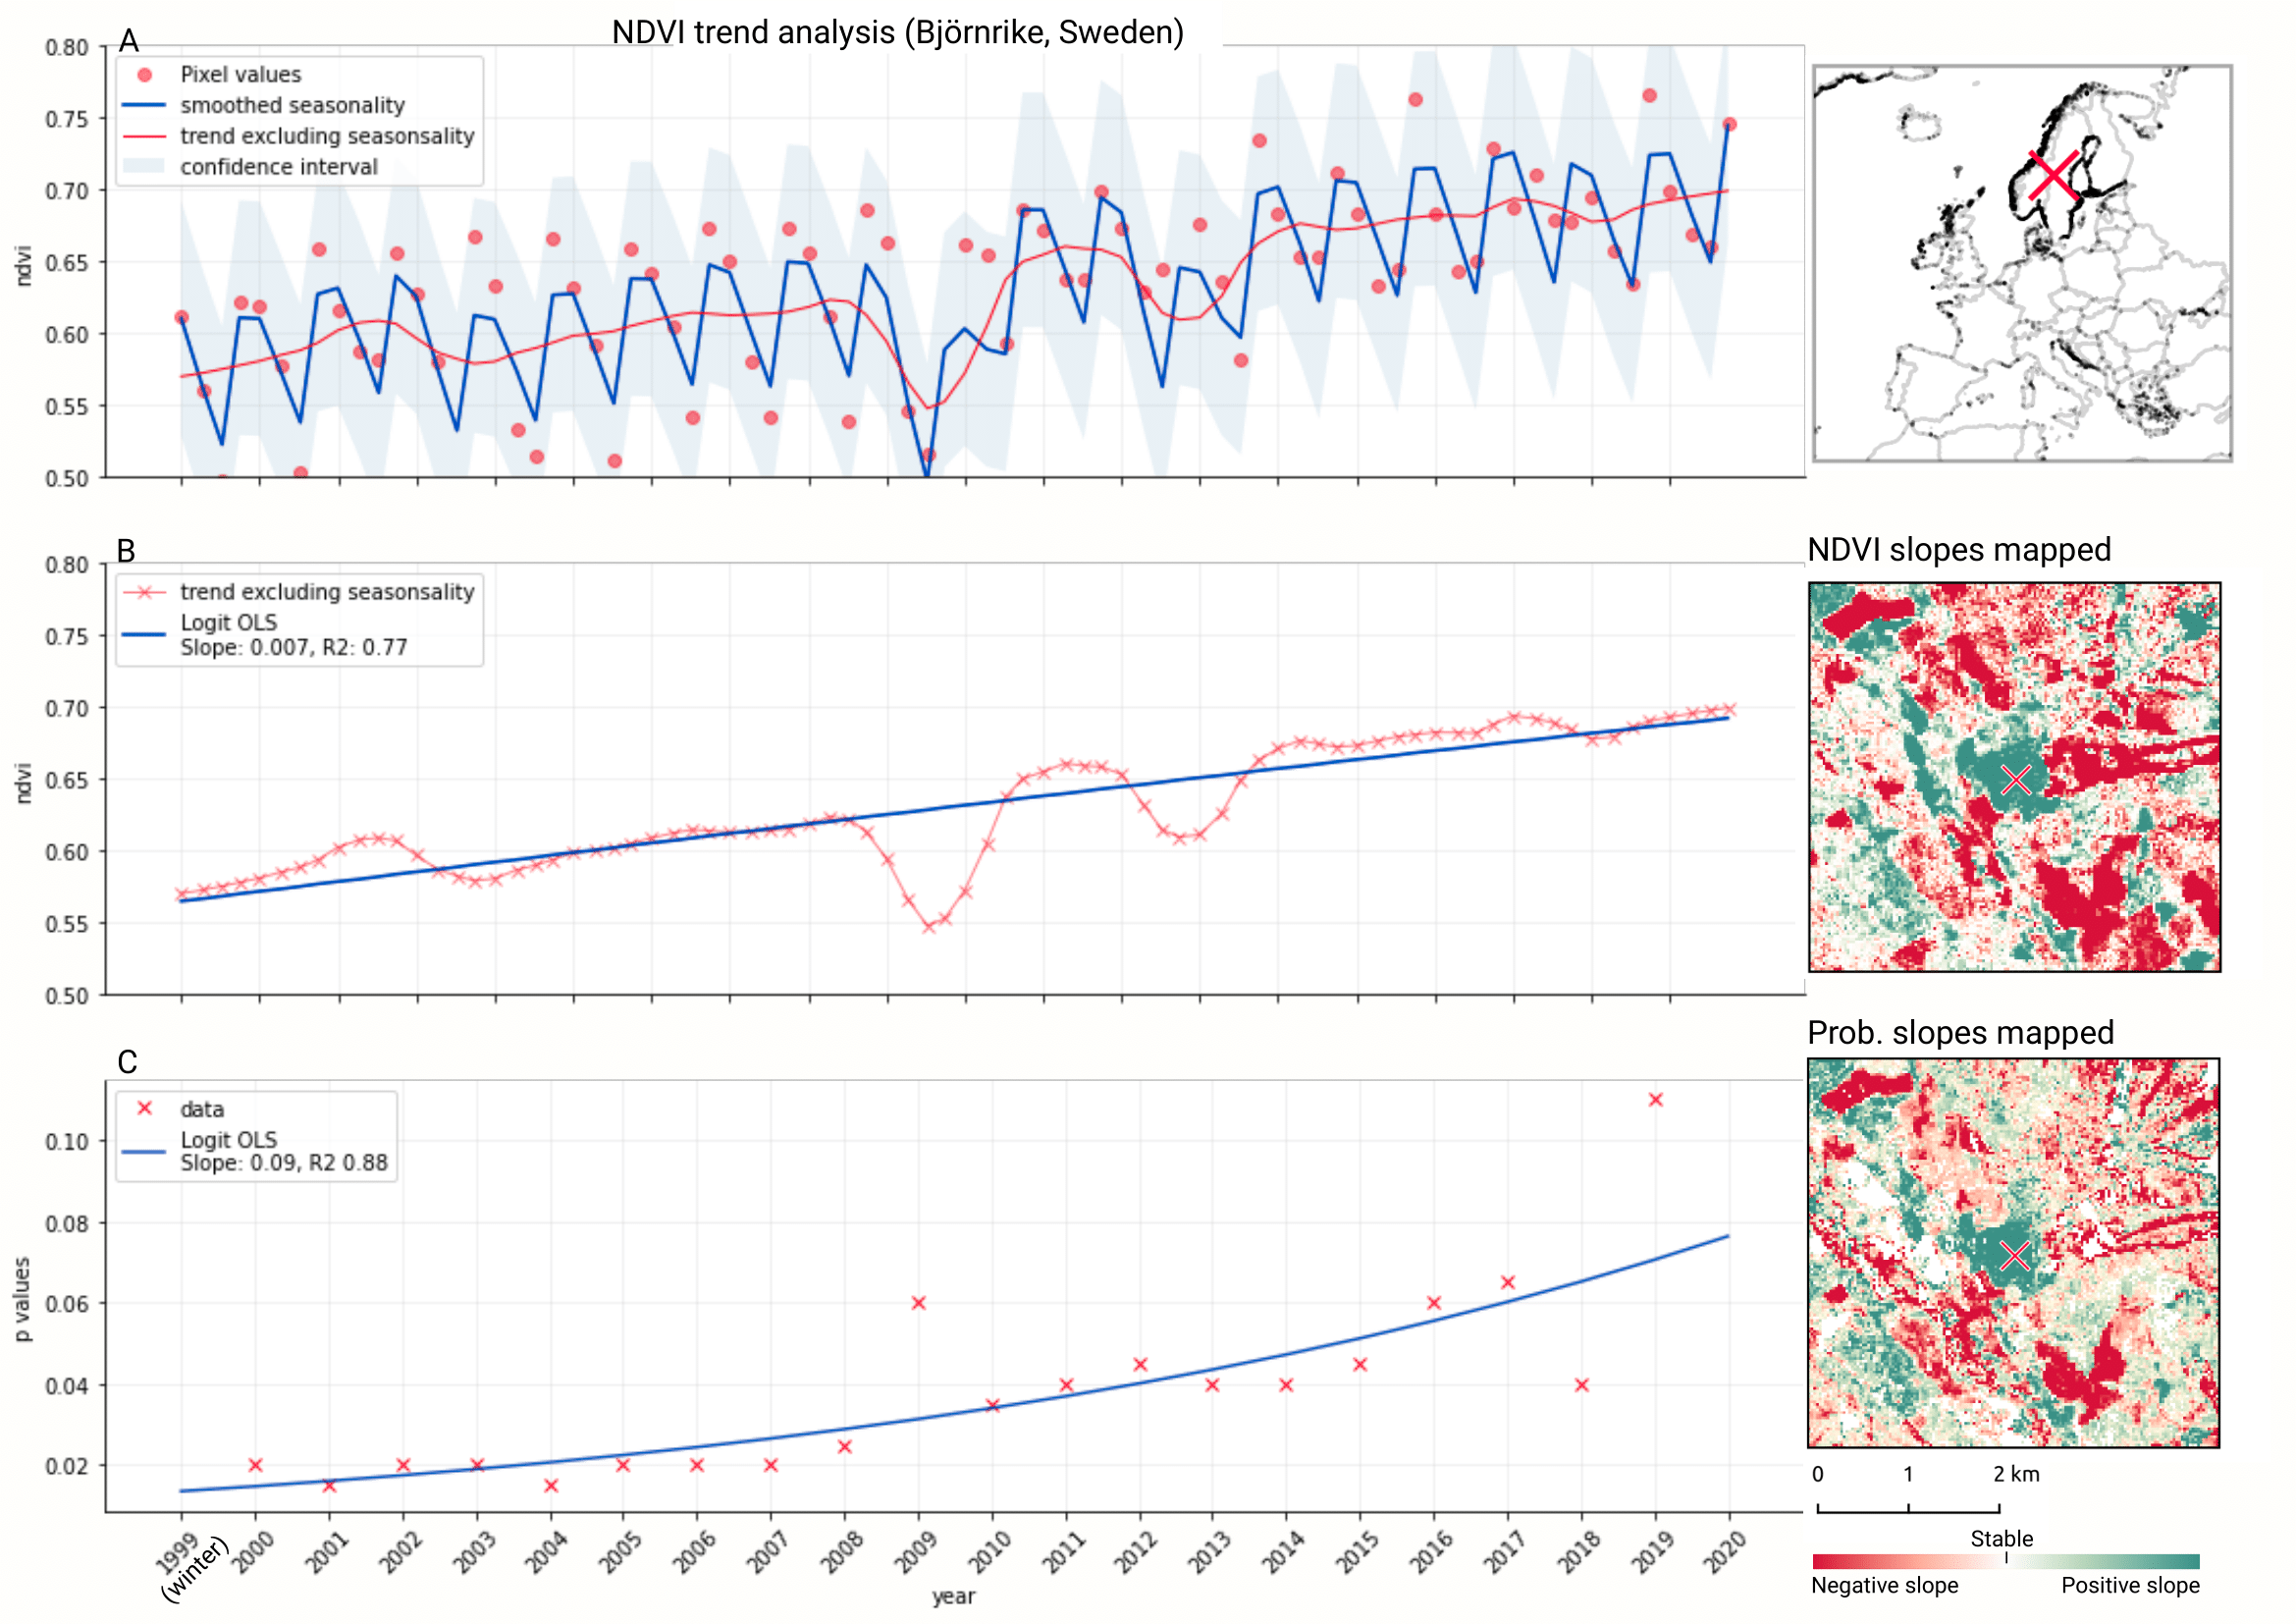
\includegraphics[width=\textwidth]{figs_03/methods_NDVI_p_slope_superplot.png}
    \caption{Example of deseasonalization \citep{seabold2010statsmodels} and subsequent Logit OLS applied on a single pixel in Sweden (Coordinates: 62{\textdegree}24'43.7"N 13{\textdegree}56'00.3"E): (a) red dots represent pixel values, the blue line represents a local weighted regression smoothed line based on the pixel values plus a light blue area indicating the confidence interval, the red line represents the trend after removing the seasonal signal; (b) red line and crosses represent the trend after removing the seasonal signal, the blue line visualizes the regression model based NDVI values in the logit space; (c) Trend analysis on probability values for non-irrigated arable land. In the case above the gradient value is 0.09 with the model R-square $=0.88$} 
    \label{fig:ndvi_timeseries}
    \end{figure}

    In order to visualise change implied by our LULC predictions, we first implement a smoothing post-processing strategy before categorizing change processes. The smoothing strategy considers the classification of a pixel in the previous and next years. If a pixel is classified as one class, but as another single class in the year before and after, this classification is considered an error. In such a case, the pixel's class is changed to match the previous and subsequent class. We call this a \emph{``T-3 temporal filter``}.
        
    After this preprocessing step, we categorize LULC change processes by applying the change classes seen in the Copernicus land cover map \citep{buchhorn2020copernicus} to our classification scheme. We translated the CLC classes to the land cover classes used by the Copernicus land cover map according to Table\@~\ref{tab:harmonization_list}. Some examples of changes include: changing from Dump sites into Urban fabric is classified as \emph{``No change''}, changing from Non-irrigated arable land into Urban fabric to \emph{``Urbanization''}, changing from Airports to Mineral extraction sites to \emph{``Other''} etc. 
    Two notable exceptions are the \emph{``forest loss''} and \emph{``Reforestation''} classes. In this paper we will refer to \emph{``Forest loss''} and \emph{``Forest increase''} instead. We renamed these change classes because we wanted to avoid making assumptions regarding the drivers of the detected trends in forest cover.
    
    In order to identify and visualize the dominant LULC change trends in Europe, we mapped the \emph{``prevalent change``} at two scales of aggregation: 5\texttimes5~km and 20\texttimes20~km. We created a Europe-covering grid with cells at both scales. Then, we counted the number of 30\texttimes30~m pixels of each change class within each grid cell. The predominant change class (see Table\@~\ref{tab:harmonization_list}) was then assigned to each grid cell. We also calculated \emph{``change intensity``} by dividing the number of 30\texttimes30~m pixels of the prevalent change class, by the sum of all pixels in each grid cell. For example, at a 20\texttimes20~km scale, each grid cell contains have $(20,000/30)\cdot (20,000/30) = ~444,444$ pixels. If the prevalent change class is present in $>$94,000 pixels this means that it covers $>$20\% of the total area. 
        
    \begin{landscape}
    \begin{table}[!hp]
    \centering
    \caption{Harmonization scheme used to convert  ODSE-LULC nomenclature to Copernicus Global Land Cover classes. On the left side,  ODSE-LULC classes are converted to Forest, Other Vegetation, Wetland, Bare, Cropland, Urban, and Water classes. Each transition from one Copernicus class to another is then categorized into a change class in the cross-table.}
    \label{tab:harmonization_list}
    \resizebox{600pt}{!}{%
    \begin{tabular}{@{}|l|l|l|l|l|l|l|l|l|@{}}
    \toprule
    \textbf{ODSE-LULC class} & \textbf{Copernicus change class} & \textbf{Forest} & \textbf{Other Vegetation} & \textbf{Wetland} & \textbf{Bare} & \textbf{Cropland} & \textbf{Urban} & \textbf{Water} \\ \midrule
    311: Broad-leaved forest & \multirow{2}{*}{\textbf{Forest}} & \multirow{2}{*}{} & \multicolumn{3}{l|}{\multirow{2}{*}{Forest loss}} & \multirow{2}{*}{\begin{tabular}[c]{@{}l@{}}Deforestation and \\ crop expansion\end{tabular}} & \multirow{2}{*}{\begin{tabular}[c]{@{}l@{}}Deforestation \\ and urbanization\end{tabular}} & \multirow{28}{*}{Water expansion} \\
    312: Coniferous forest &  &  & \multicolumn{3}{l|}{} &  &  &  \\ \cmidrule(r){1-8}
    321: Natural grasslands & \multirow{4}{*}{\textbf{Other Vegetation}} & \multirow{26}{*}{Reforestation} & \multirow{4}{*}{} & \multirow{4}{*}{Other} & \multirow{4}{*}{Desertification} & \multirow{4}{*}{Crop expansion} & \multirow{4}{*}{Urbanization} &  \\
    322: Moors and heathland &  &  &  &  &  &  &  &  \\
    324: Transitional woodland-shrub &  &  &  &  &  &  &  &  \\
    323: Sclerophyllous vegetation &  &  &  &  &  &  &  &  \\ \cmidrule(r){1-2} \cmidrule(lr){4-8}
    411: Inland wetlands & \multirow{2}{*}{\textbf{Wetland}} &  & \multirow{2}{*}{Wetland degradation} & \multirow{2}{*}{} & \multirow{2}{*}{\begin{tabular}[c]{@{}l@{}}Wetland degradation \\ and desertification\end{tabular}} & \multirow{2}{*}{\begin{tabular}[c]{@{}l@{}}Wetland degradation \\ and crop expansion\end{tabular}} & \multirow{2}{*}{\begin{tabular}[c]{@{}l@{}}Wetland degradation \\ and urbanization\end{tabular}} &  \\
    421: Maritime wetlands &  &  &  &  &  &  &  &  \\ \cmidrule(r){1-2} \cmidrule(lr){4-8}
    332: Bare rocks & \multirow{5}{*}{\textbf{Bare}} &  & \multicolumn{2}{l|}{\multirow{5}{*}{Other}} & \multirow{5}{*}{} & \multirow{5}{*}{Crop expansion} & \multirow{12}{*}{Urbanization} &  \\
    333: Sparsely vegetated areas &  &  & \multicolumn{2}{l|}{} &  &  &  &  \\
    334: Burnt areas &  &  & \multicolumn{2}{l|}{} &  &  &  &  \\
    335: Glaciers and perpetual snow &  &  & \multicolumn{2}{l|}{} &  &  &  &  \\
    335: Beaches, dunes, and sands &  &  & \multicolumn{2}{l|}{} &  &  &  &  \\ \cmidrule(r){1-2} \cmidrule(lr){4-7}
    211: Non-irrigated arable land & \multirow{7}{*}{\textbf{Cropland}} &  & \multicolumn{2}{l|}{\multirow{7}{*}{Land abandonment}} & \multirow{7}{*}{\begin{tabular}[c]{@{}l@{}}Land abandonment \\ and desertification\end{tabular}} & \multirow{7}{*}{} &  &  \\
    212: Permanently irrigated arable land &  &  & \multicolumn{2}{l|}{} &  &  &  &  \\
    213: Rice fields &  &  & \multicolumn{2}{l|}{} &  &  &  &  \\
    221: Vineyards &  &  & \multicolumn{2}{l|}{} &  &  &  &  \\
    222: Fruit trees and berry plantations &  &  & \multicolumn{2}{l|}{} &  &  &  &  \\
    223: Olive groves &  &  & \multicolumn{2}{l|}{} &  &  &  &  \\
    231: Pastures &  &  & \multicolumn{2}{l|}{} &  &  &  &  \\ \cmidrule(r){1-2} \cmidrule(lr){4-8}
    111: Urban fabric & \multirow{8}{*}{\textbf{Urban}} &  & \multicolumn{4}{l|}{\multirow{8}{*}{Other}} & \multirow{8}{*}{} &  \\
    122: Road and rail networks and associated land &  &  & \multicolumn{4}{l|}{} &  &  \\
    123: Port areas &  &  & \multicolumn{4}{l|}{} &  &  \\
    124: Airports &  &  & \multicolumn{4}{l|}{} &  &  \\
    131: Mineral extraction sites &  &  & \multicolumn{4}{l|}{} &  &  \\
    132: Dump sites &  &  & \multicolumn{4}{l|}{} &  &  \\
    133: Construction sites &  &  & \multicolumn{4}{l|}{} &  &  \\
    141: Green urban areas &  &  & \multicolumn{4}{l|}{} &  &  \\ \midrule
    511: Water courses & \multirow{5}{*}{\textbf{Water}} & \multicolumn{6}{l|}{\multirow{5}{*}{Water reduction}} & \multirow{5}{*}{} \\
    512: Water bodies &  & \multicolumn{6}{l|}{} &  \\
    523: Sea and ocean &  & \multicolumn{6}{l|}{} &  \\
    522: Estuaries &  & \multicolumn{6}{l|}{} &  \\
    521: Coastal lagoons &  & \multicolumn{6}{l|}{} &  \\ \bottomrule
    \end{tabular}%
    }
    \end{table}
    \end{landscape}

\section{Results}

\subsection*{Quality of reference data}
    %\emph{Edited by: Luka Antonić}

    Table\@~\ref{tab:odse-lulc-pts_vs_other_lulc_products} shows how well each compared land cover product matched  ODSE-LULC training data. The comparison with S2GLC with our points from 2016 and 2018 resulted in the highest F1-scores, while the land cover product made by \citet{pflugmacher2019mapping} fits more closely to the 2015 subset (0.657). The 2019 point subset was considered too small to perform any meaningful comparison between  ELC10 and GLFCS30. The number of classes can vary per dataset per year because we excluded all classes from the translated dataset that do not appear in the target land cover product.
    
    \begin{table}[!hbt]
    \centering
    \caption{Weighted F1-score of other land cover products when validated with the ODSE-LULC training dataset.}
    \label{tab:odse-lulc-pts_vs_other_lulc_products}
    \begin{tabular}{@{}lrlrrrr@{}}
    \toprule
    Land cover product & \multicolumn{1}{l}{\begin{tabular}[c]{@{}l@{}}Validation \\ year\end{tabular}} & \begin{tabular}[c]{@{}l@{}}Data \\ source\end{tabular} & \multicolumn{1}{l}{Samples} & \multicolumn{1}{l}{\begin{tabular}[c]{@{}l@{}}Weighted \\ F1-Score\end{tabular}} & \multicolumn{1}{l}{\begin{tabular}[c]{@{}l@{}}Number of \\ classes\end{tabular}} & \multicolumn{1}{l}{\begin{tabular}[c]{@{}l@{}} Res.\@ (m)\end{tabular}} \\ \midrule
    
    S2GLC & 2016 & LUCAS & 756 & 0.724 & 8 & 10 \\
    \citet{pflugmacher2019mapping} & 2016 & LUCAS & 719 & 0.719 & 10 & 30 \\
    GLFCS30--2015 & 2016 & LUCAS & 724 & 0.677 & 10 & 30 \\
    \citet{pflugmacher2019mapping} & 2015 & LUCAS & 144,027 & 0.657 & 11 & 30 \\
    S2GLC & 2018 & LUCAS & 295,152 & 0.653 & 11 & 10 \\
    S2GLC & 2018 & CLC & 1,000,063 & 0.604 & 12 & 10 \\
     ELC10 & 2018 & LUCAS & 42,629 & 0.596 & 8 & 10 \\
    GLFCS30--2015 & 2015 & LUCAS & 138,342 & 0.503 & 12 & 30 \\
     ELC10 & 2018 & CLC & 172,382 & 0.456 & 8 & 10 \\
    GLFCS30--2020 & 2018 & LUCAS & 308,838 & 0.424 & 12 & 30 \\
    GLFCS30--2020 & 2018 & CLC & 1,026,914 & 0.420 & 12 & 30 \\ \bottomrule
    \end{tabular}


    \end{table}

\subsection*{Spatiotemporal ensemble modelling results}

    The EML model optimization resulted in the following hyperparameters and architecture:
    \begin{itemize}
    \item Random forest: Number of trees equal to 85, maximum depth per tree equal to 25, number of variables to find the best split equal to 89, and 20 as minimum number of samples per leaf.  
    \item Gradient boosted trees:  Number of boosting rounds equal to 28, maximum depth per tree equal to 7, minimum loss reduction necessary to split a leaf node equal to 1, L1 regularization term on weights equal to 0.483, learning rate equal to 0.281, greedy histogram algorithm to construct the trees, and \textsf{softmax} as objective function. 
    \item Artificial Neural Network: Four fully connected hidden layers with 64 artificial neurons each; \textsf{ReLU} as activation function,  dropout rate equal to 0.15 and batch normalization in all the layers;  \textsf{softmax} as activation function for output layer; batch size and number of epochs equal to 64 and 50, respectively; and Adam with Nesterov momentum as optimizer considering  5e-4 as learning rate.
    \item Logistic Regression: SAGA solver and multinomial function to minimize the loss.
    \end{itemize}

    The variable importance, generated by the two tree-based learners and presented in Fig.\@~\ref{fig:variable_importance}, shows that the 50th quantile for summer and winter of the Landsat green band were most important to the random forest and gradient boosted tree models, respectively. In addition to spectral bands, several Landsat-derived spectral indices (NBR2, SAVI, NDVI, REI, NDWI, MSAVI appear amongst the 40 most important variables. Global surface water frequency was the third most important for the random forest. Fig.\@~\ref{fig:variable_importance} also shows that the summer aggregates of Landsat green (25th quantile) and NDVI are the two most important variables where the highest importance among the two models is less than double the importance of the other model. Except for Landsat green and NDVI, most variables were found important by only one model. For instance, the geometric temperatures and nighttime land surface temperatures were only important for the random forest. The differences in variable importance indicate that the component models use different parts of the feature space before their predictions are combined by the meta-learner, suggesting that ensembles can utilize a wider proportion of the feature space than single models.
    
    \begin{figure}[!hp]
    \centering
    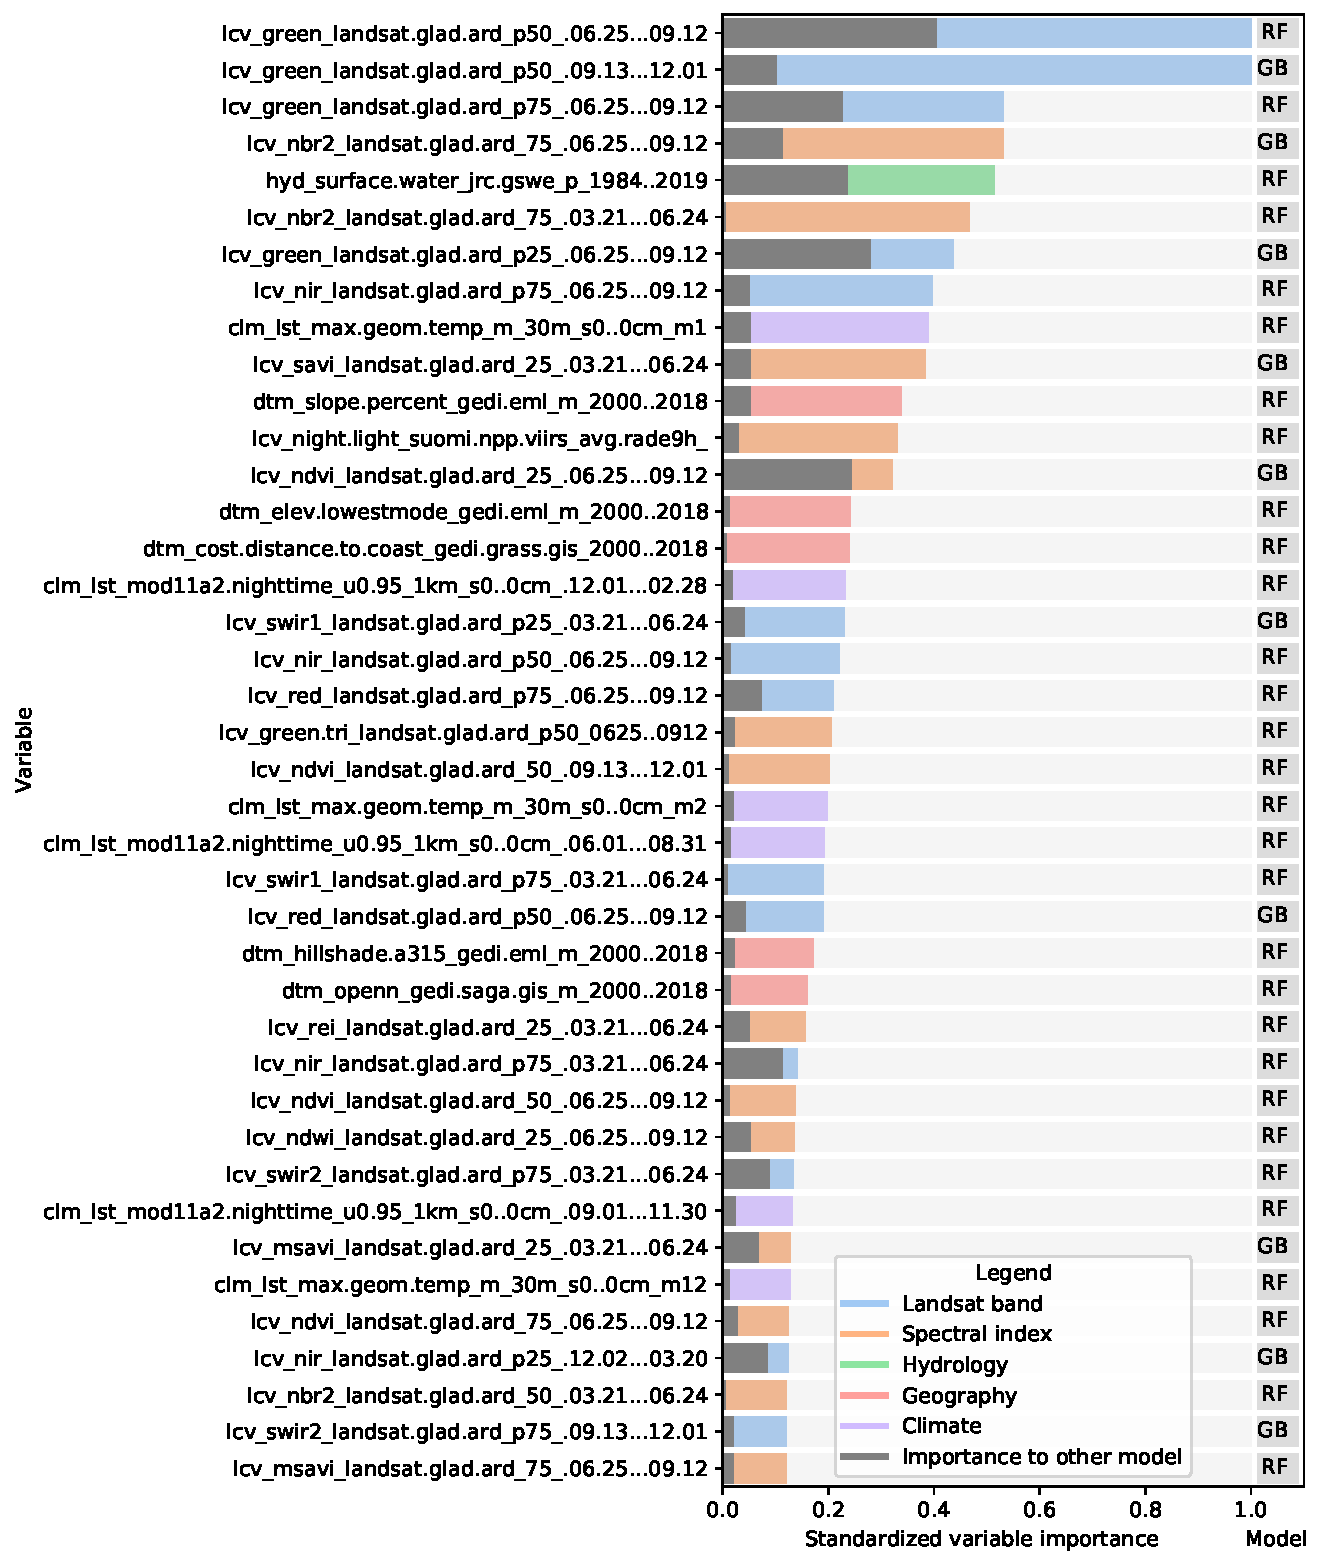
\includegraphics[width=\textwidth]{figs_03/results_variable_importance.pdf}
    \caption{Standardized importance of the top-40 most important variables to the random forest and gradient boosted tree models. The colored bar indicates the highest importance of the variable among the two models. This model is indicated to the right of each bar. The corresponding grey bar indicates the importance to the other model. The color of each bar indicates the data type. Each variable name is prefixed with either LCV (either part of a Landsat band or a landsat-derived spectral index), HYD (Hydrological data), CLM (climatic data), or DTM (digital terrain model). This prefix is followed by the specific data source, e.g. \emph{[color or index]\_landsat} indicates a Landsat band or derived spectral index. The last part of each name indicates the timespan over which the data was aggregated.}
    \label{fig:variable_importance}
    \end{figure}
        

\subsection*{Accuracy assessment results}

    \subsubsection*{Spatial cross-validation}
        
        We performed 5-fold spatial cross-validation with the final hyperparameters for our ensemble. The predictions on the left-out folds were aggregated to assess model performance on the entire dataset. Table\@~\ref{tab:cv_level} shows that the model achieved higher weighted user and producer accuracy, as well as F1-score and log loss ratio, when predictions were aggregated to their next level in the CLC hierarchy. Table\@~\ref{tab:cv_accuracy_lvl3} shows that the model only achieved an F1-score over 0.5 for 10 out of 43 classes (112, 121,211,213,311,312,332,335,412,512). The model performed best when predicting 512: Water bodies (0.924), 335: Glaciers and perpetual snow (0.834), and 412: Peat bogs (0.707). It achieved the lowest F1-scores for 334: Burnt areas (0.011), 132: Dump sites (0.026) and 133: Construction sites (0.065). However, log loss ratios for each class and each CLC level overall were higher than 0, indicating that the model assigned probabilities more accurately than a random classifier even for the most difficult classes.
        
        When the predictions were aggregated to 14 level 2 classes (see Table\@~\ref{tab:cv_accuracy_lvl2}), the model performed best when classifying 51: Inland waters (0.924), 31: Forests and seminatural areas (0.813) and 41: Inland wetlands (0.708). The biggest increase in performance through aggregation to level 2 was in 31: Forests, as the weighted average F1-score of its subclasses (311,312,313) was 0.553. The least accurately predicted classes were 14: Artificial, non-agricultural vegetated areas (0.308), 13: Mine, dump and construction sites (0.370) and 22: Permanent crops (0.412).
    
        Table\@~\ref{tab:cv_accuracy_lvl1} shows that at the highest level of aggregation with 5 general classes, the model classified 5: Water bodies most accurately (0.926) and 1: Artificial surfaces the least (0.688). The best performance improvement from aggregation was for 2: Agricultural areas, as the weighted average F1-score of its subclasses (21, 22, 23, 24) was 0.546, but increased with 0.279 upon aggregation.

        \begin{table}[!hbt]
        \centering
        \caption{Producer's and user's accuracy, Weighted F1-score, and Log loss of the ensemble predictions during spatial cross-validation. }
        \label{tab:cv_level}
        \resizebox{\textwidth}{!}{%
        \begin{tabular}{@{}lrrrrrrr@{}}
        \toprule
        Corine level & \begin{tabular}[c]{@{}l@{}}Number \\ of classes\end{tabular} & Prod acc. & User acc. & Weighted F1 & Log Loss & Baseline Log Loss & Log Loss Ratio\\ 
        \midrule
        1 & 5  & 0.835 & 0.835 & 0.834 & 0.456 & 2.018 & 0.774 \\
        2 & 14 & 0.636 & 0.639 & 0.509 & 1.033 & 3.596 & 0.713 \\
        3 & 43 & 0.494 & 0.502 & 0.491 & 1.544 & 5.142 & 0.700 \\ 
        \bottomrule
        \end{tabular}
        }
        \end{table}

        \begin{table}[!hbt]
        \centering
        \caption{Classification report for 43 CLC level 3 classes, based on the predictions made with 5-fold spatial cross-validation.}
        \label{tab:cv_accuracy_lvl3}
        \resizebox{\textwidth}{!}{%
        \begin{tabular}{lrrrrrrr}
        \toprule
        CLC code (level 3)         & Producer Acc. & User Acc. & F1-score & Support & Log loss & Baseline Log Loss & Log Loss Ratio \\ 
        \midrule
        111: Continuous urban fabric                            & 0.523         & 0.166     & 0.252    &  51,989        & 0.0230        & 0.0388        & 0.409 \\
        112: Discontinuous urban fabric                         & 0.509         & 0.572     & 0.539    &  92,151        & 0.0256        & 0.0623        & 0.590 \\
        121: Industrial or commercial units                     & 0.496         & 0.623     & 0.552    & 129,661        & 0.0382        & 0.0821        & 0.535 \\
        122: Road and rail networks and associated land         & 0.294         & 0.068     & 0.111    &  39,832        & 0.0244        & 0.0311        & 0.213 \\
        123: Port areas                                         & 0.543         & 0.321     & 0.403    &   3,994        & 0.0018        & 0.0042        & 0.578 \\
        124: Airports                                           & 0.300         & 0.023     & 0.043    &   6,702        & 0.0049        & 0.0067        & 0.265 \\
        131: Mineral extraction sites                           & 0.482         & 0.307     & 0.375    &  53,447        & 0.0264        & 0.0397        & 0.335 \\
        132: Dump sites                                         & 0.375         & 0.013     & 0.026    &   6,509        & 0.0048        & 0.0065        & 0.267 \\
        133: Construction sites                                 & 0.217         & 0.038     & 0.065    &   6,728        & 0.0047        & 0.0067        & 0.299 \\
        141: Green urban areas                                  & 0.312         & 0.125     & 0.179    &  15,717        & 0.0091        & 0.0141        & 0.350 \\
        142: Sport and leisure facilities                       & 0.407         & 0.200     & 0.268    &  64,308        & 0.0326        & 0.0463        & 0.297 \\
        211: Non-irrigated arable land                          & 0.604         & 0.733     & 0.662    & 998,381        & 0.1892        & 0.3735        & 0.493 \\
        212: Permanently irrigated arable land                  & 0.447         & 0.146     & 0.221    &  29,786        & 0.0139        & 0.0243        & 0.428 \\
        213: Rice fields                                        & 0.762         & 0.496     & 0.601    &   4,839        & 0.0020        & 0.0050        & 0.596 \\
        221: Vineyards                                          & 0.506         & 0.308     & 0.383    &  66,213        & 0.0287        & 0.0474        & 0.394 \\
        222: Fruit trees and berry plantations                  & 0.411         & 0.131     & 0.199    &  63,659        & 0.0344        & 0.0459        & 0.251 \\
        223: Olive groves                                       & 0.432         & 0.355     & 0.390    &  63,578        & 0.0244        & 0.0459        & 0.469 \\
        231: Pastures                                           & 0.455         & 0.529     & 0.489    & 529,466        & 0.1509        & 0.2415        & 0.375 \\
        241: Annual crops associated with permanent crops       & 0.269         & 0.067     & 0.107    &  16,883        & 0.0101        & 0.0150        & 0.326 \\
        242: Complex cultivation patter                         & 0.348         & 0.351     & 0.349    & 594,648        & 0.1942        & 0.2624        & 0.260 \\
        243: Agriculture with significant natural vegetation    & 0.355         & 0.373     & 0.363    & 782,237        & 0.2558        & 0.3176        & 0.194 \\
        244: Agro-forestry areas                                & 0.276         & 0.052     & 0.087    &  10,497        & 0.0060        & 0.0099        & 0.396 \\
        311: Broad-leaved forest                                & 0.537         & 0.660     & 0.592    & 855,499        & 0.1971        & 0.3373        & 0.416 \\
        312: Coniferous forest                                  & 0.596         & 0.646     & 0.620    & 759,215        & 0.1644        & 0.3112        & 0.472 \\
        313: Mixed forest                                       & 0.461         & 0.377     & 0.414    & 612,430        & 0.1707        & 0.2680        & 0.363 \\
        321: Natural grasslands                                 & 0.406         & 0.314     & 0.354    & 400,875        & 0.1431        & 0.1971        & 0.274 \\
        322: Moors and heathland                                & 0.493         & 0.350     & 0.409    & 301,693        & 0.1100        & 0.1591        & 0.309 \\
        323: Sclerophyllous vegetation                          & 0.311         & 0.372     & 0.339    & 143,521        & 0.0532        & 0.0890        & 0.403 \\
        324: Transitional woodland-shrub                        & 0.472         & 0.431     & 0.450    & 724,404        & 0.2117        & 0.3013        & 0.297 \\
        331: Beaches, dunes, sand                               & 0.551         & 0.207     & 0.301    &  25,688        & 0.0147        & 0.0214        & 0.312 \\
        332: Bare rocks                                         & 0.664         & 0.495     & 0.567    &  58,234        & 0.0162        & 0.0427        & 0.621 \\
        333: Sparsely vegetated areas                           & 0.522         & 0.471     & 0.495    & 152,571        & 0.0457        & 0.0935        & 0.511 \\
        334: Burnt areas                                        & 0.224         & 0.006     & 0.011    &   2,263        & 0.0021        & 0.0026        & 0.177 \\
        335: Glaciers and perpetual snow                        & 0.852         & 0.818     & 0.834    &   7,250        & 0.0008        & 0.0072        & 0.883 \\
        411: Inland marshes                                     & 0.425         & 0.228     & 0.297    &  39,784        & 0.0192        & 0.0310        & 0.382 \\
        412: Peat bogs                                          & 0.684         & 0.731     & 0.707    & 174,314        & 0.0333        & 0.1039        & 0.680 \\
        421: Salt marshes                                       & 0.505         & 0.441     & 0.471    &   5,598        & 0.0023        & 0.0057        & 0.600 \\
        422: Salines                                            & 0.481         & 0.081     & 0.139    &     320        & 0.0002        & 0.0004        & 0.577 \\
        423: Intertidal flats                                   & 0.497         & 0.209     & 0.295    &     788        & 0.0004        & 0.0010        & 0.570 \\
        511: Water courses                                      & 0.360         & 0.108     & 0.166    &  11,214        & 0.0068        & 0.0105        & 0.353 \\
        512: Water bodies                                       & 0.895         & 0.956     & 0.924    & 187,981        & 0.0108        & 0.1103        & 0.902 \\
        521: Coastal lagoons                                    & 0.594         & 0.429     & 0.498    &   1,904        & 0.0006        & 0.0022        & 0.708 \\
        522: Estuaries                                          & 0.382         & 0.082     & 0.135    &     353        & 0.0002        & 0.0005        & 0.566 \\
        \midrule
        Macro average    & 0.460         & 0.327     & 0.356    & \multicolumn{1}{c}{\multirow{2}{*}{8097140}} & 0.083 & 0.137 & 0.452 \\
        Weighted average & 0.494         & 0.502     & 0.491    & \multicolumn{1}{c}{} & 0.157 & 0.253 & 0.389 \\ 
        \midrule
        Accuracy         & \multicolumn{4}{l}{0.502}                      \\
        Kappa score      & \multicolumn{4}{l}{0.459}                      \\ 
        Log Loss (baseline) & \multicolumn{4}{l}{1.544 (5.142)}                      \\
        \bottomrule
        \end{tabular}%
        }
        \end{table}
        
        \begin{table}[!hbt]
        \centering
        \caption{Classification report for 14 CLC level 2 classes, based on the predictions made with 5-fold spatial cross-validation.}
        \label{tab:cv_accuracy_lvl2}
        \resizebox{\textwidth}{!}{%
        \begin{tabular}{lrrrrrrr}
        \toprule
        CLC code (level 2)      & Producer Acc. & User Acc. & f1-score & Support & Log Loss & Baseline Log Loss & Log Loss Ratio                                     \\ 
        \midrule
        11: Urban Fabric             						& 0.643 & 0.535 & 0.584	&   144,140	& 0.039 & 0.089 & 0.564 \\
        12: Industrial, commercial and transport units      & 0.568 & 0.551 & 0.559	&   180,189	& 0.057 & 0.107 & 0.469 \\
        13: Mine, dump and construction sites             	& 0.533 & 0.283 & 0.370	&    66,684	& 0.032 & 0.048 & 0.331 \\
        14: Artificial, non-agricultural vegetated areas    & 0.479 & 0.227 & 0.308	&    80,025	& 0.038 & 0.055 & 0.315 \\
        21: Arable land               						& 0.622 & 0.738 & 0.675	& 1,033,006	& 0.191 & 0.382 & 0.500 \\
        22: Permanent crops             					& 0.558 & 0.326 & 0.412	&   193,450	& 0.072 & 0.113 & 0.363 \\
        23: Pastures             							& 0.455 & 0.529 & 0.489	&   529,466	& 0.151 & 0.242 & 0.375 \\
        24: Heterogeneous agricultural areas               	& 0.488 & 0.496 & 0.492	& 1,404,265	& 0.364 & 0.461 & 0.212 \\
        31: Forests and seminatural areas               	& 0.788 & 0.840 & 0.813	& 2,227,144	& 0.302 & 0.588 & 0.487 \\
        32: Shrub and/or herbaceous vegetation associations	& 0.592 & 0.511 & 0.548	& 1,570,493	& 0.384 & 0.492 & 0.218 \\
        33: Open spaces with little or no vegetation        & 0.736 & 0.591 & 0.656	&   246,006	& 0.061 & 0.136 & 0.555 \\
        41: Inland wetlands            						& 0.719 & 0.697 & 0.708	&   214,098	& 0.044 & 0.122 & 0.643 \\
        42: Coastal wetlands             					& 0.591 & 0.465 & 0.520	&     6,706	& 0.003 & 0.007 & 0.618 \\
        51: Inland waters             						& 0.913 & 0.936 & 0.924	&   199,195	& 0.013 & 0.115 & 0.884 \\
        52: Marine waters             						& 0.614 & 0.392 & 0.479	&     2,273	& 0.001 & 0.003 & 0.699 \\
        \midrule
        Macro average    & 0.620         & 0.541     & 0.569    & \multicolumn{1}{c}{\multirow{2}{*}{8,097,140}} & 0.117 & 0.197 & 0.482 \\
        Weighted average & 0.636         & 0.639     & 0.634    & \multicolumn{1}{c}{} & 0.262 & 0.420 & 0.393                        \\ 
        \midrule
        Accuracy         & \multicolumn{4}{l}{0.639}                                                           \\
        Kappa score       & \multicolumn{4}{l}{0.565}                                                           \\
        Log Loss (baseline) & \multicolumn{4}{l}{1.033 (3.596)}                      \\
        \bottomrule
        \end{tabular}%
        }
        \end{table}

        \begin{table}[!hbt]
        \centering
        \caption{Classification report for 5 CLC level 1 classes, based on the predictions made with 5-fold spatial cross-validation.}
        \label{tab:cv_accuracy_lvl1}
        \resizebox{\textwidth}{!}{%
        \begin{tabular}{lrrrrrrr}
        \toprule
        CLC code (level 1) &  Producer Acc. &  User Acc. &  F1-score &  Support & Log Loss & Baseline Log Loss & Log Loss Ratio \\
        \midrule
        1: Artificial surfaces          & 0.784 & 0.613 & 0.688 &   471,038 & 0.123 & 0.222 & 0.445 \\
        2: Agricultural areas           & 0.798 & 0.854 & 0.825 & 3,160,187 & 0.457 & 0.669 & 0.317 \\
        3: Forest and seminatural areas	& 0.872 & 0.848 & 0.860 & 4,043,643 & 0.526 & 0.693 & 0.241 \\
        4: Wetlands            			& 0.722 & 0.696 & 0.708 &   220,804 & 0.045 & 0.125 & 0.639 \\
        5: Water bodies            		& 0.917 & 0.936 & 0.926 &   201,468 & 0.013 & 0.116 & 0.884 \\
        \midrule
        Macro average    &          0.819 &      0.789 &     0.802 & \multicolumn{1}{c}{\multirow{2}{*}{8,097,140}} & 0.233 & 0.365 & 0.505 \\
        Weighted average &          0.835 &      0.835 &     0.834 & \multicolumn{1}{c}{} & 0.450 & 0.626 &	0.309 \\
        \midrule
        Accuracy     & \multicolumn{4}{l}{0.835} \\
        Kappa score        & \multicolumn{4}{l}{0.720} \\
        Log Loss (baseline)         & \multicolumn{4}{l}{0.456 (2.018)} \\
        \bottomrule
        \end{tabular}
        }
        \end{table}
        
        We calculated a separate weighted F1-score for each tile that was used for spatial cross-validation to investigate spatial patterns in classification performance. The average weighted F1-score per tile was 0.463, with a standard deviation of 0.150. Fig.\@~\ref{fig:cv_spatial} shows a disparity in performance between northern and southern Europe. Fig.\@~\ref{fig:tiles_support_vs_v1} shows that there is a significant correlation (0.125, p=0.000) between the number of reference points and the weighted F1 score of a tile.
        
        \begin{figure}[!hp]
        \centering
        \includegraphics[width=\linewidth]{figs_03/results_study_area_tiled.pdf}
        \caption{30~km tiling system used for spatial cross-validation, showing the number of samples per tile (left) and the cross-validation weighted F1-score per tile (right).}
        \label{fig:cv_spatial}
        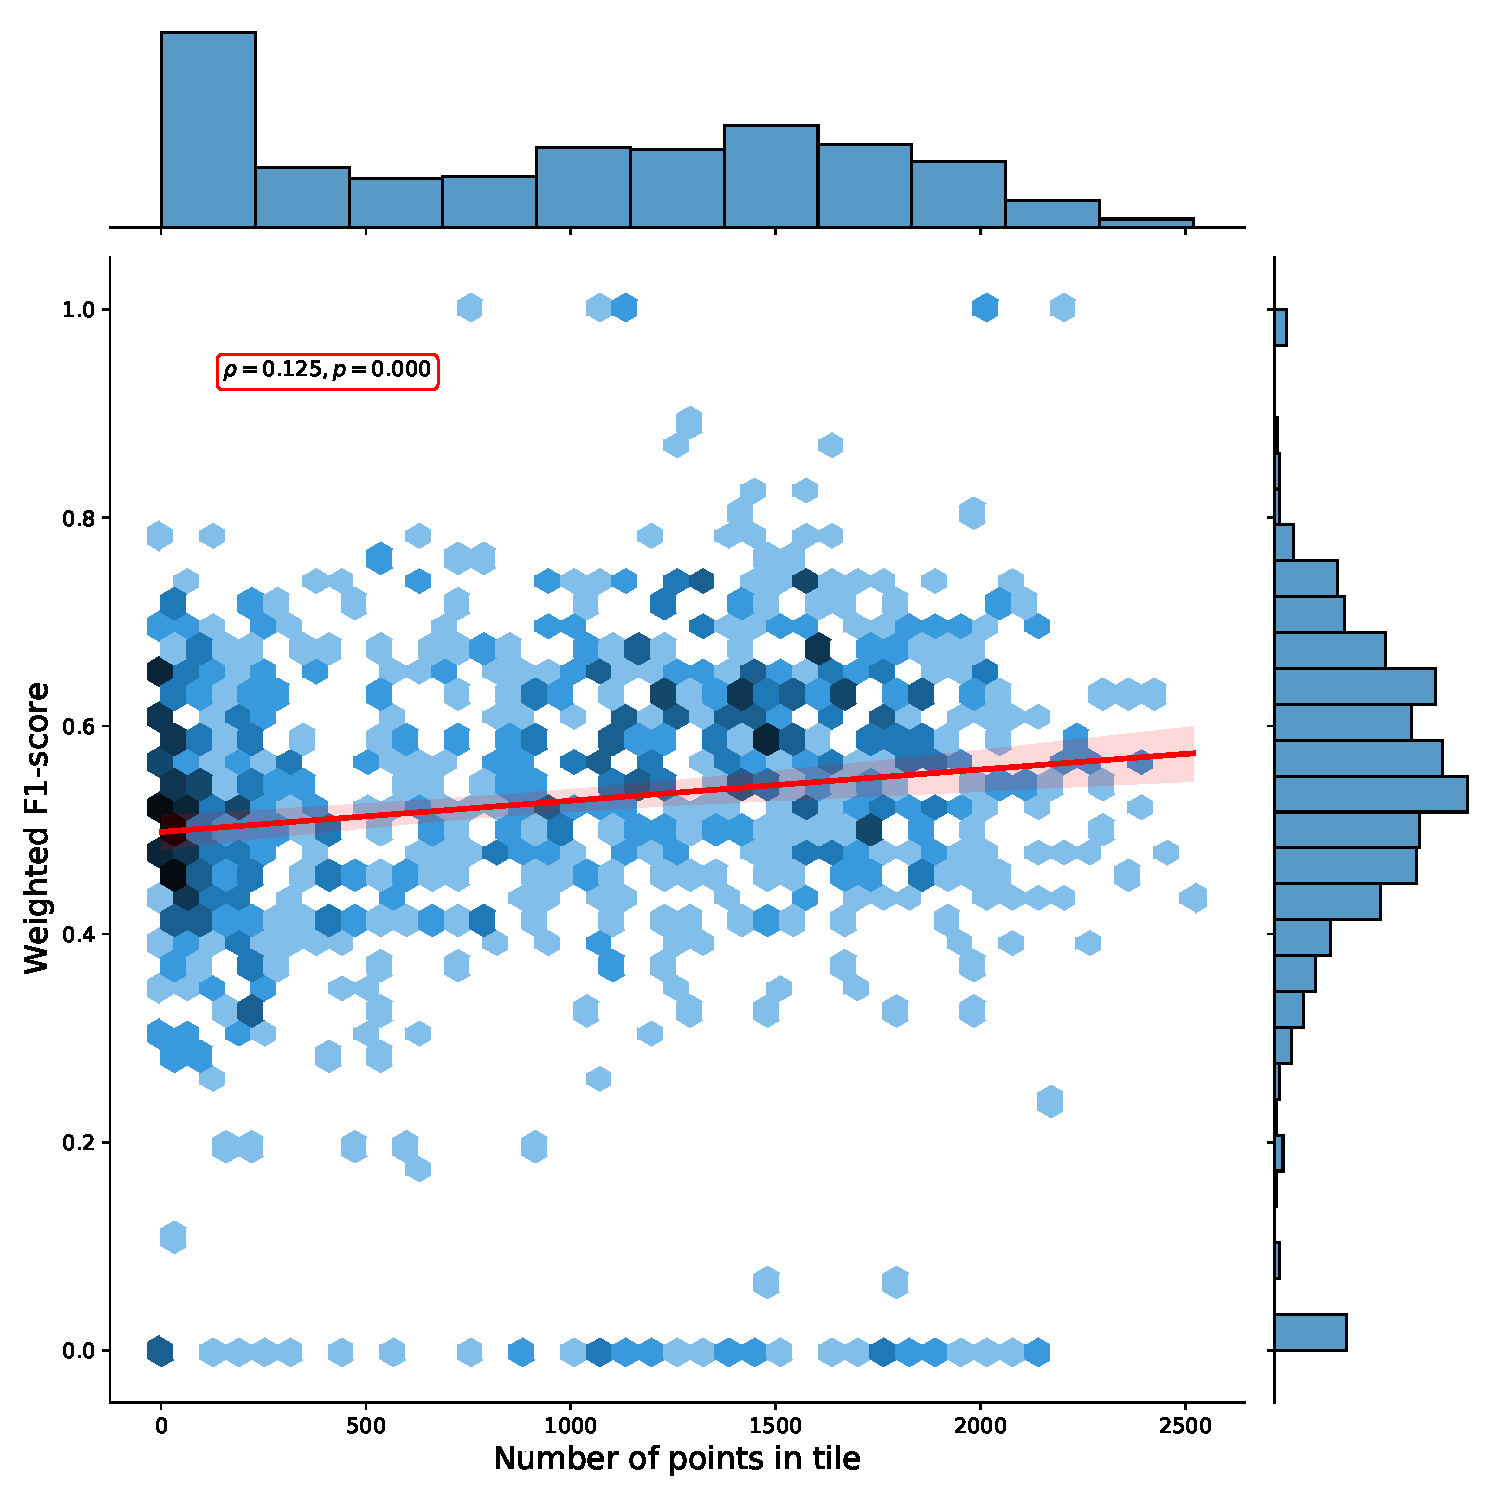
\includegraphics[width=.75\linewidth]{figs_03/results_tiles_support_vs_f1.pdf}
        \caption{Hexbin plot of the weighted F1-score and number of overlapping points per tile. The Pearson correlation coefficient of 0.125 (p: 0.000) indicates there is a weak positive correlation between the number of points in a tile and the cross-validation weighted F1-score.}
        \label{fig:tiles_support_vs_v1}
        \end{figure}
        
        We calculated a separate weighted F1-score for all cross-validation predictions from each separate year. Table\@~\ref{tab:cv_annual} shows that the average weighted F1-score per year was 0.489 with a standard deviation of 0.135. It only scored higher than 0.5 on years with less than 1~million points.
        
        \begin{table}[!hbt]
        \centering
        \caption{Cross-validation performance of our ensemble model per year.}
        \label{tab:cv_annual}
        \begin{tabular}{lrr}
        \toprule
        Year &  Weighted F1-score &  Support \\
        \midrule
        2000 &              0.497 &  1,658,715 \\
        2006 &              0.491 &  1,852,645 \\
        2009 &              0.558 &   225,416 \\
        2012 &              0.487 &  1,971,812 \\
        2015 &              0.588 &   265,830 \\
        2016 &              0.632 &    65,235 \\
        2018 &              0.481 &  2,057,306 \\
        2019 &              0.535 &      180 \\
        \midrule
        Average &              0.489 &  1,012,142 \\
        Standard deviation &              0.135 &   882,783 \\
        \bottomrule
        \end{tabular}
        \end{table}
    
        
    \subsubsection*{Validation on S2GLC points}
        \label{sec:results-s2glc}
        We validated the ensemble on S2GLC dataset.
        We overlaid 49,897 S2GLC points with our input variables for 2017 and classified 43 LULC classes with our model. These 43-class predictions were reclassified to the S2GLC nomenclature. 3,484 points had a predicted class that was not in the S2GLC nomenclature (see Table\@~\ref{tab:malinowski_keys}). The \emph{`conservative'} assessment (on all 49,897 points) including the non-S2GLC classes resulted in a weighted F1-score of 0.854 and a kappa score of 0.794 (see Table\@~\ref{tab:classification_report_s2glc_conservative}). The \emph{`optimistic`} assessment excluding non-S2GLC predictions resulted in a weighted F1-score of 0.889 and a kappa score of 0.867 (see Table\@~\ref{tab:classification_report_s2glc_optimistic}). 

        Taking into account possible noise from the translation process, these results are similar to those reported by \citet{malinowski2020}. Weighted average user and producer accuracy and F1-scores are also higher than our cross-validation scores at all thematic resolution levels (see Table\@~\ref{tab:cv_level}). They are also higher than what we obtained when we transformed our cross-validation predictions to the S2GLC nomenclature, which yielded a weighted F1-score 0.611 and a kappa score of 0.535.
        
        \begin{table}[!hbt]
        \centering
        \caption{Conservative classification report of our 2017 LULC prediction on 49,897 S2GLC points that counts 3484 points with predicted classes without an equivalent S2GLC class as errors (141: Green urban areas, 142: Sport and leisure facilities, 222: Fruit trees and berry plantations, 223: Olive groves, 313: Mixed forest, 324: Transitional woodland-shrub, 333: Sparsely vegetated areas, and 334: Burnt areas).}
        \label{tab:classification_report_s2glc_conservative}
        \begin{tabular}{@{}lrrrr@{}}
        \toprule
        S2GLC Class                      & \multicolumn{1}{l}{Producer Acc.} & \multicolumn{1}{l}{User Acc.} & \multicolumn{1}{l}{F1-score} & \multicolumn{1}{l}{Support} \\ 
        \midrule
        111: Artificial surfaces       & 0.933                             & 0.933                         & 0.933                        & 1,826                    \\
        211: Cultivated areas          & 0.849                             & 0.965                         & 0.903                        & 13,470                   \\
        221: Vineyards                 & 0.826                             & 0.694                         & 0.754                        & 500                     \\
        231: Herbaceous vegetation     & 0.861                             & 0.686                         & 0.764                        & 6,776                    \\
        311: Broadleaf tree cover      & 0.967                             & 0.814                         & 0.884                        & 10,944                   \\
        312: Coniferous tree cover     & 0.975                             & 0.914                         & 0.943                        & 8,626                    \\
        322: Moors and heathland       & 0.641                             & 0.491                         & 0.556                        & 2,070                    \\
        323: Sclerophyllous vegetation & 0.780                             & 0.265                         & 0.396                        & 815                     \\
        331: Natural material surfaces & 0.915                             & 0.751                         & 0.825                        & 2,110                    \\
        335: Permanent snow cover      & 0.624                             & 0.800                         & 0.701                        & 85                      \\
        411: Marshes                   & 0.331                             & 0.327                         & 0.329                        & 324                     \\
        412: Peatbogs                  & 0.629                             & 0.482                         & 0.546                        & 745                     \\
        511: Water bodies              & 0.992                             & 0.974                         & 0.983                        & 1,606                    \\
        \midrule
        Macro average                   & 0.737                             & 0.650                         & 0.680                        & \multirow{2}{*}{49,897}      \\
        Weighted average                & 0.892                             & 0.830                         & 0.854                        &                             \\
        \midrule
        Accuracy                        & 0.830                             & \multicolumn{1}{l}{}          & \multicolumn{1}{l}{}         & \multicolumn{1}{l}{}        \\
        Kappa score                     & 0.794                             & \multicolumn{1}{l}{}          & \multicolumn{1}{l}{}         & \multicolumn{1}{l}{}        \\ 
        \bottomrule
        \end{tabular}
        \end{table}
        
        \begin{table}[!hbt]
        \centering
        \caption{Optimistic classification report of our 2017 LULC prediction on 49,897 S2GLC points where all 3484 points with predicted classes without an equivalent S2GLC class were removed before calculating accuracy metrics (141: Green urban areas, 142: Sport and leisure facilities, 222: Fruit trees and berry plantations, 223: Olive groves, 313: Mixed forest, 324: Transitional woodland-shrub, 333: Sparsely vegetated areas, and 334: Burnt areas).}
        \label{tab:classification_report_s2glc_optimistic}
        \begin{tabular}{@{}lrrrr@{}}
        \toprule
        S2GLC Class                      & \multicolumn{1}{l}{Producer Acc.} & \multicolumn{1}{l}{User Acc.} & \multicolumn{1}{l}{F1-score} & \multicolumn{1}{l}{Support} \\
        \midrule
        111 : Artificial surfaces       & 0.933                             & 0.935                         & 0.934                        & 1,823                    \\
        211 : Cultivated areas          & 0.849                             & 0.967                         & 0.905                        & 13,429                   \\
        221 : Vineyards                 & 0.826                             & 0.720                         & 0.769                        & 482                     \\
        231 : Herbaceous vegetation     & 0.861                             & 0.722                         & 0.785                        & 6,441                    \\
        311 : Broadleaf tree cover      & 0.967                             & 0.937                         & 0.952                        & 9,512                    \\
        312 : Coniferous tree cover     & 0.975                             & 0.973                         & 0.974                        & 8,098                    \\
        322 : Moors and heathland       & 0.641                             & 0.672                         & 0.656                        & 1,511                    \\
        323 : Sclerophyllous vegetation & 0.780                             & 0.378                         & 0.509                        & 571                     \\
        331 : Natural material surfaces & 0.915                             & 0.866                         & 0.889                        & 1,831                    \\
        335 : Permanent snow cover      & 0.624                             & 0.819                         & 0.708                        & 83                      \\
        411 : Marshes                   & 0.331                             & 0.351                         & 0.341                        & 302                     \\
        412 : Peatbogs                  & 0.629                             & 0.494                         & 0.554                        & 726                     \\
        511 : Water bodies              & 0.992                             & 0.975                         & 0.984                        & 1,604                    \\
        \midrule
        Macro average                   & 0.794                             & 0.755                         & 0.766                        & \multirow{2}{*}{46,413}      \\
        Weighted average                & 0.893                             & 0.892                         & 0.889                        &                             \\
        \midrule
        Accuracy                        & 0.892                             & \multicolumn{1}{l}{}          & \multicolumn{1}{l}{}         & \multicolumn{1}{l}{}        \\
        Kappa score                     & 0.867                             & \multicolumn{1}{l}{}          & \multicolumn{1}{l}{}         & \multicolumn{1}{l}{}       \\
        \bottomrule
        \end{tabular}
        \end{table}
        
        Fig.\@~\ref{fig:confusion_matrix_s2glc_independent} shows a normalized confusion matrix of our validation on the S2GLC dataset. It shows the rate at which each true class (rows) was predicted as each other class (columns). The diagonal cells report the true positive rate of each class. Class 000 represents classes not present in the S2GLC dataset; as there were no ground truth points in the dataset with these classes, the top row of the matrix is empty. The matrix shows that, when normalized for support, the biggest sources of error were the incorrect classification of classes 323: Sclerophyllous vegetation and 322: Moors and Heathland as classes not in the S2GLC dataset with 29.9\% and 27.0\% of all errors for these classes, respectively, and of 411: Marshes as 231: Herbaceous vegetation (28.4\%). We include a similar confusion matrix of our cross-validation predictions (Fig.\@~\ref{fig:confusion_matrix_s2glc_crossvalidated}, transformed to the S2GLC nomenclature, to allow a comparison between our cross-validation and independent validation. It shows that many classes have a higher true positive rate in the independent validation on S2GLC points than in our cross-validation results, except for 211: Cultivated areas, 335: Permanent snow cover, and 412: Peatbogs.
        
        \begin{figure}[!hbt]
            \centering
            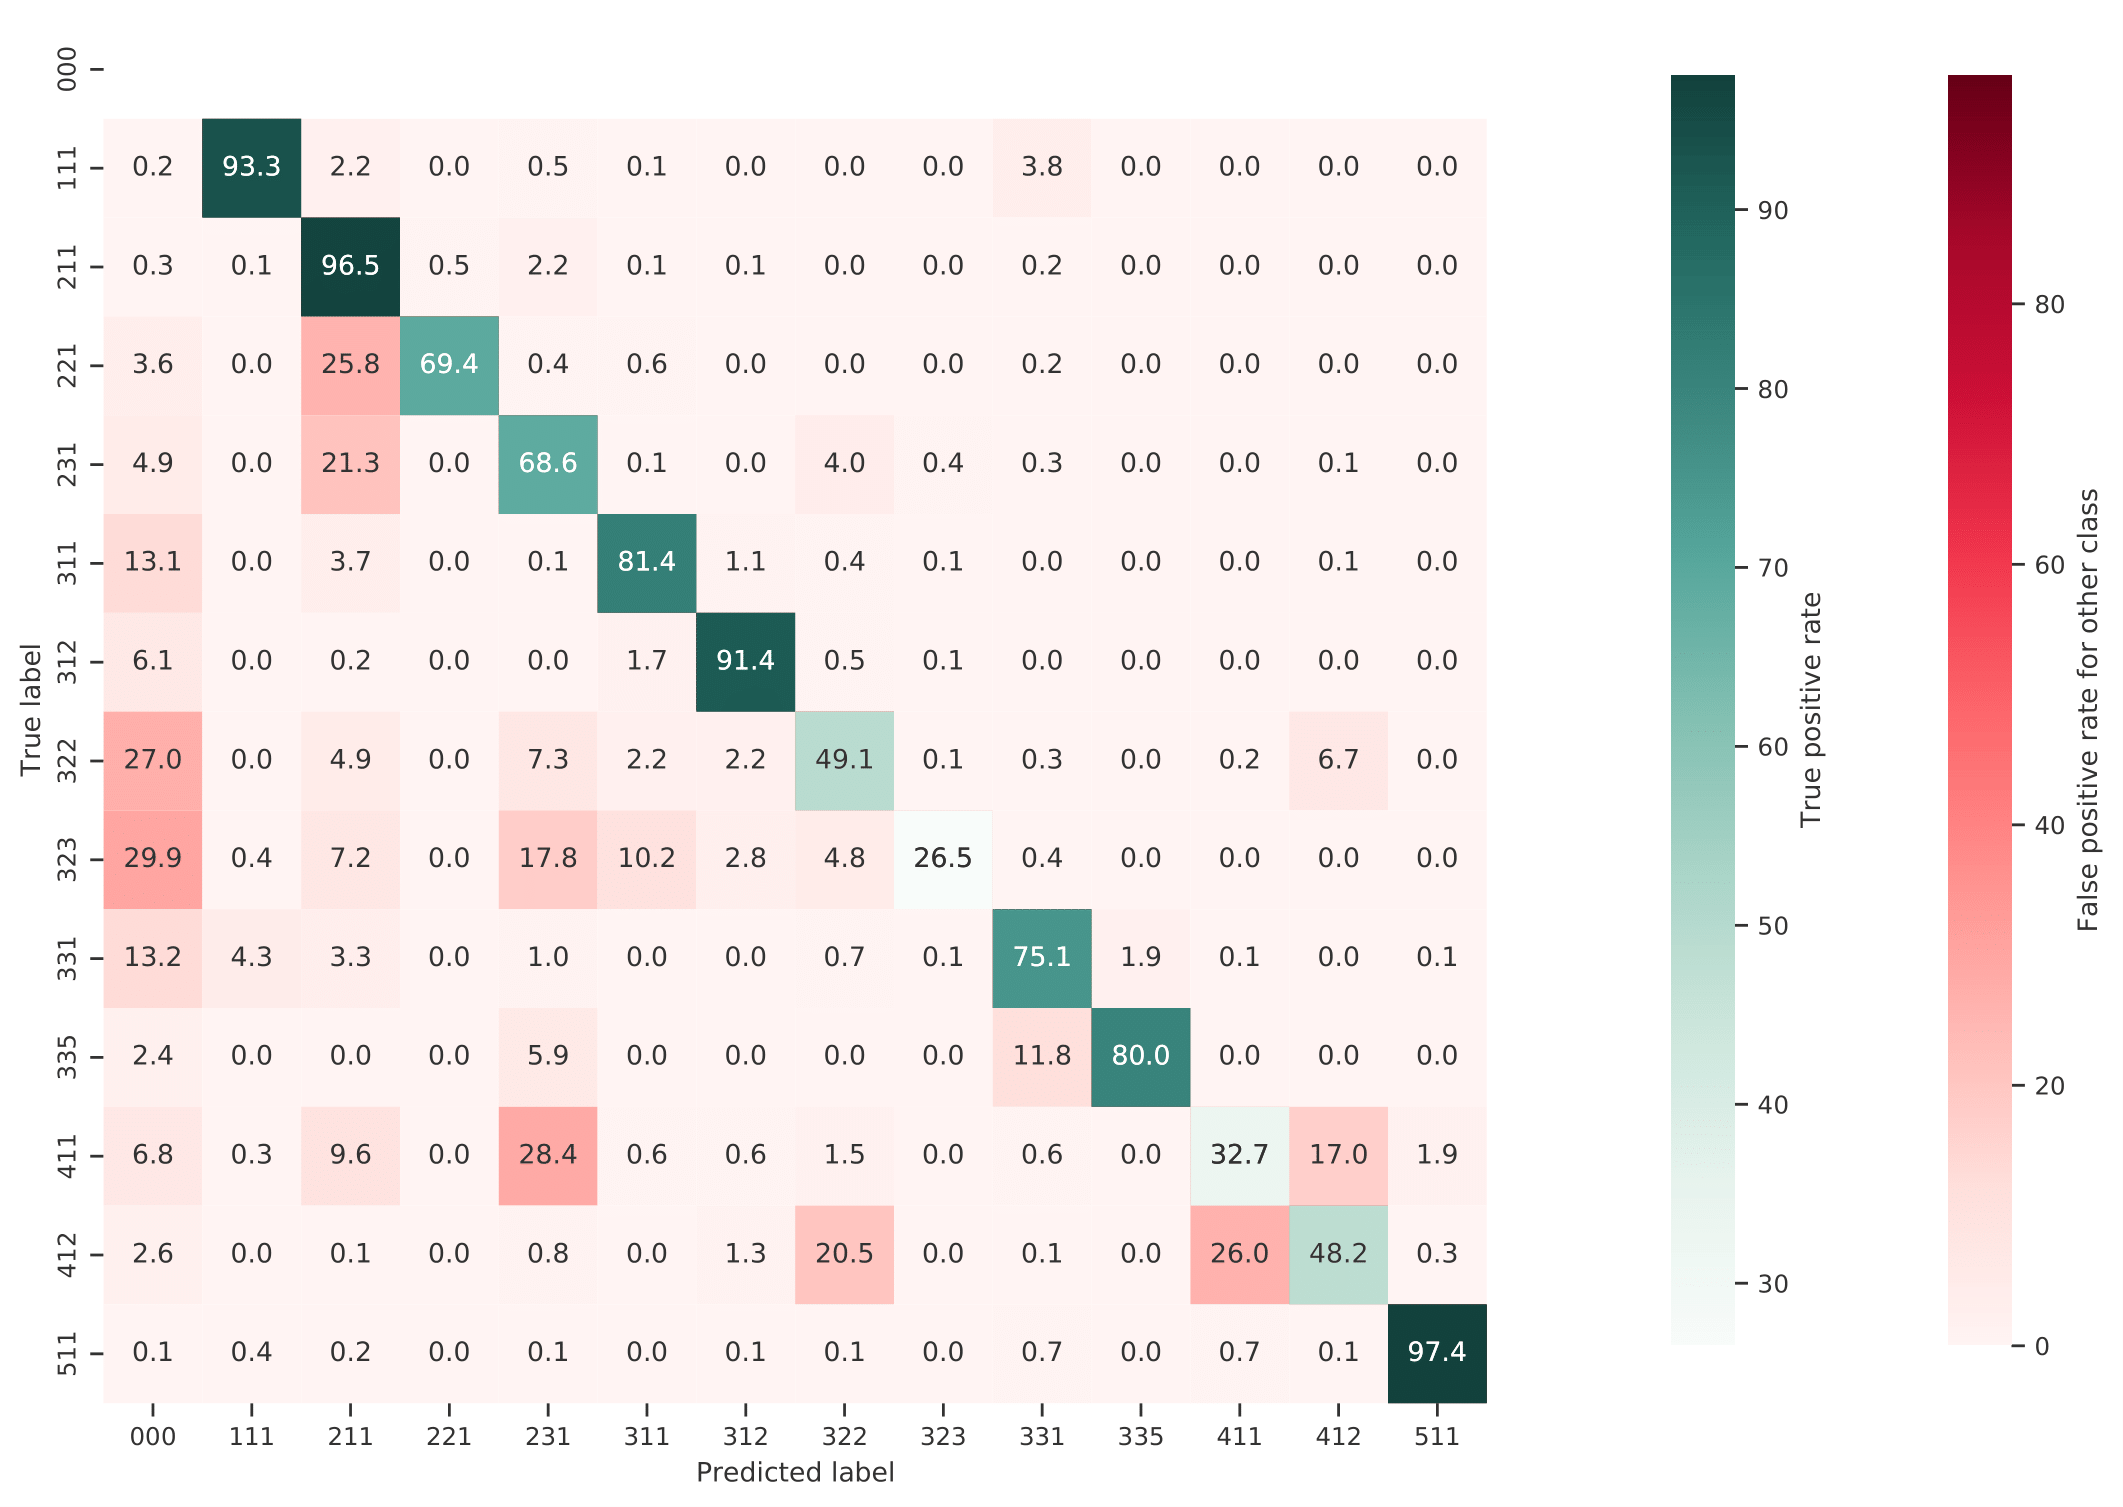
\includegraphics[width=0.95\textwidth]{figs_03/results_confusion_matrix_s2glc_conservative_predicted_rate.png}
            \caption{Normalized confusion matrix of our prediction on the independently collected S2GLC validation points. Each cell shows the percentage of the true label predicted as the predicted label.}
            \label{fig:confusion_matrix_s2glc_independent}
            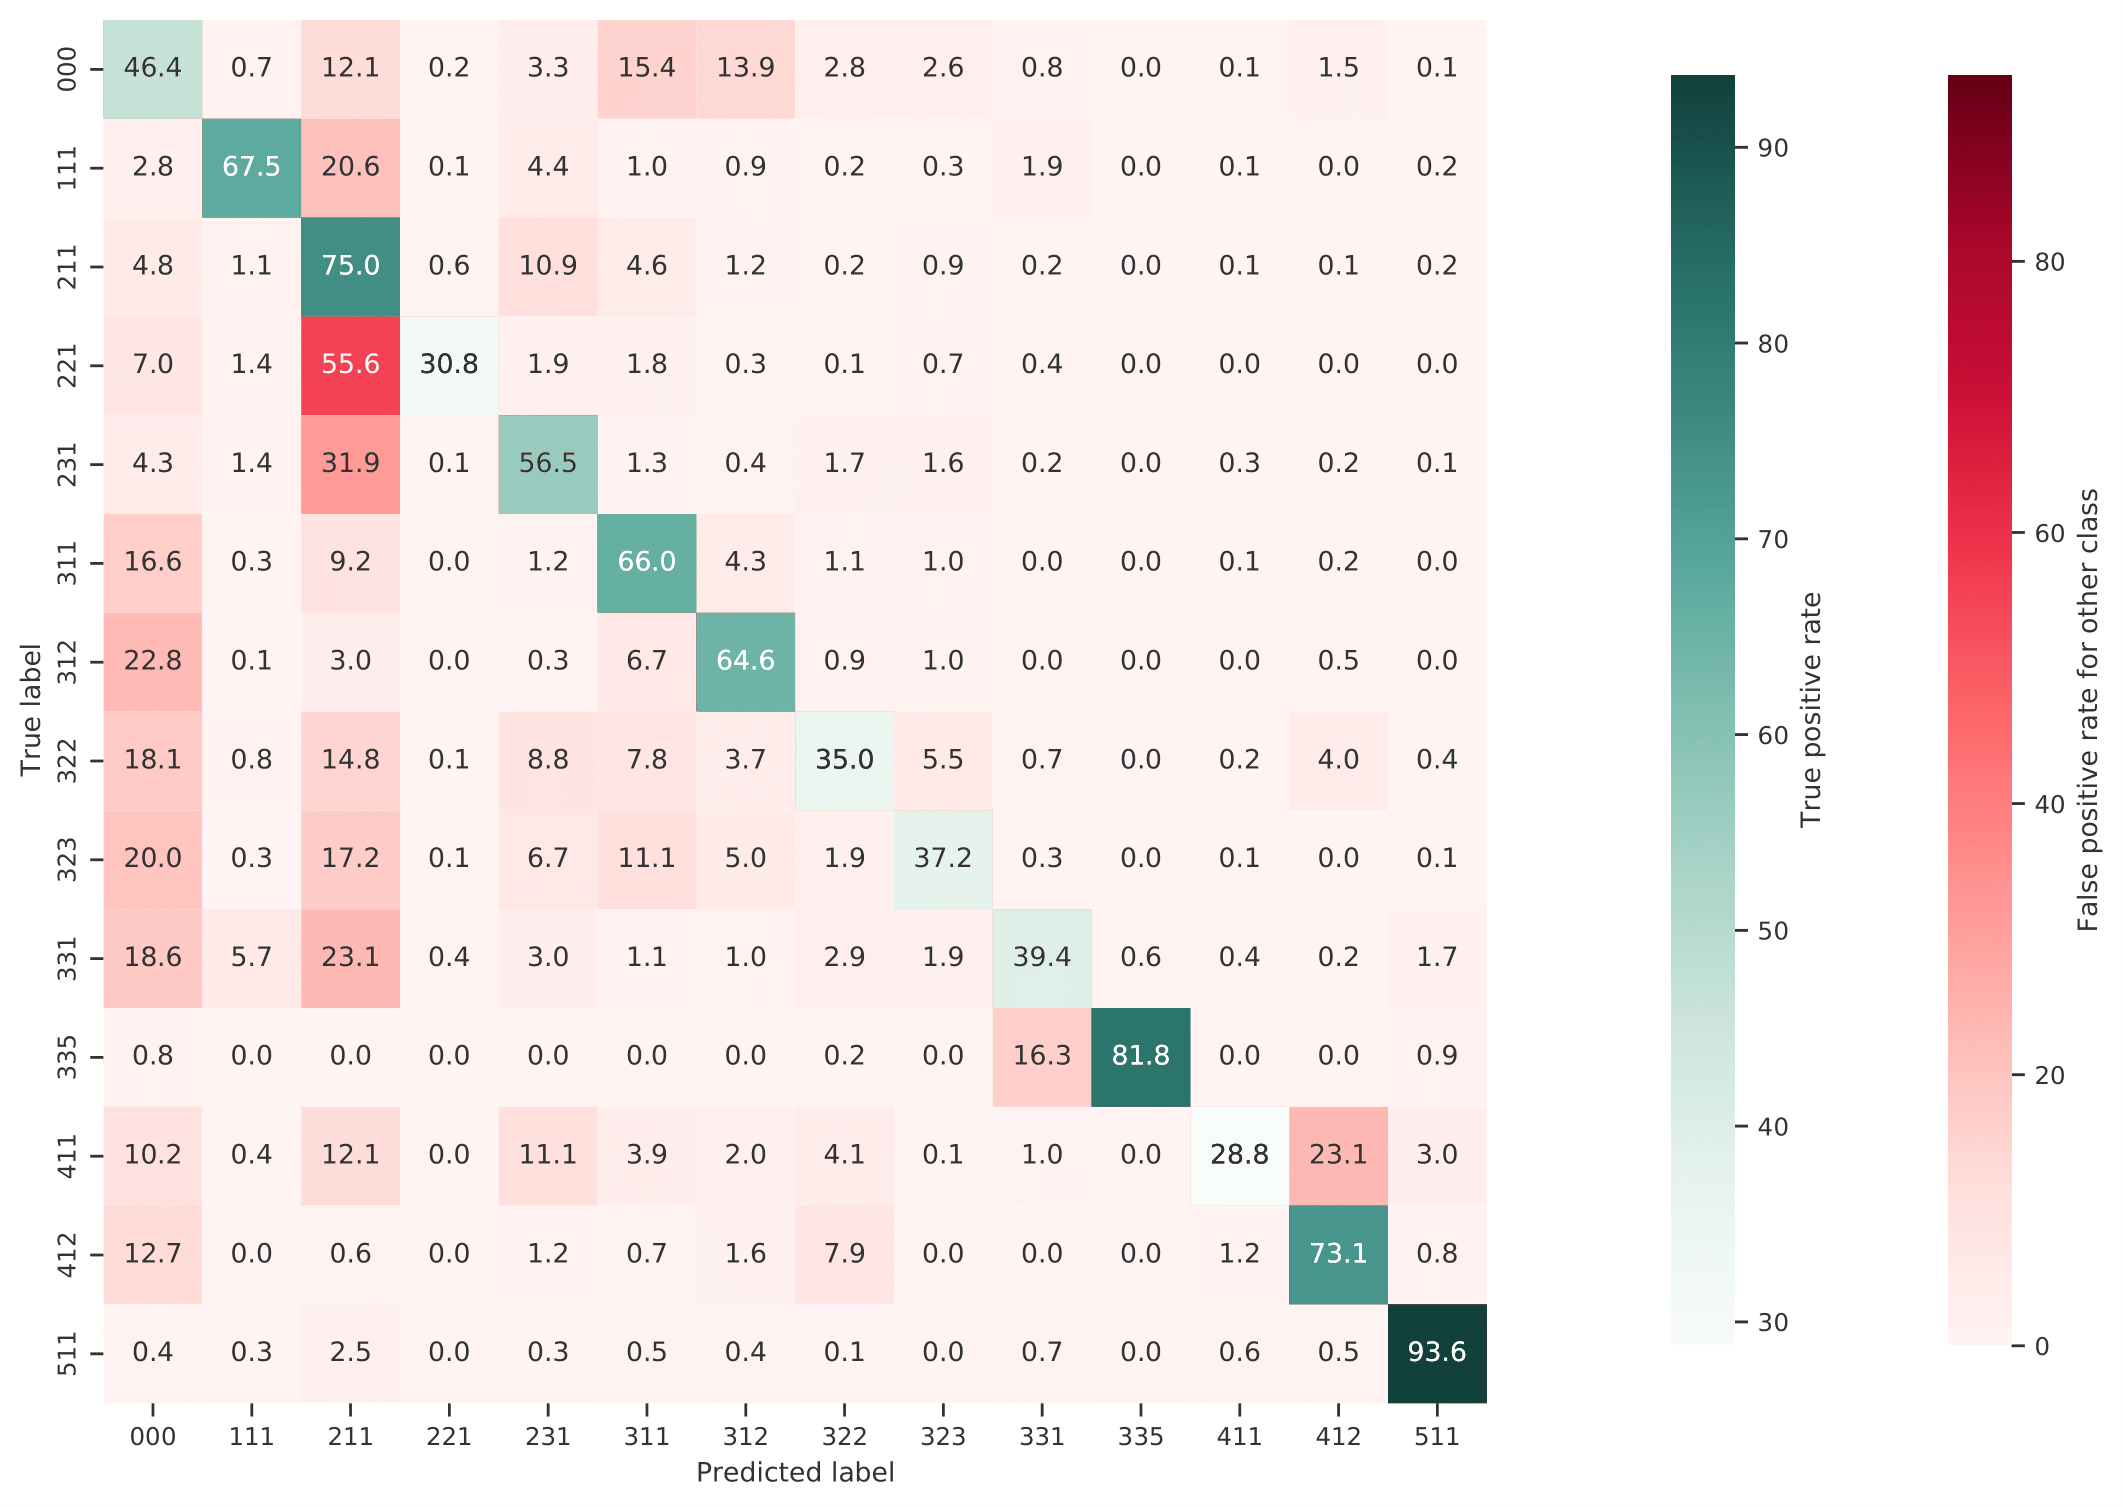
\includegraphics[width=0.95\textwidth]{figs_03/results_confusion_matrix_s2glc-CV_conservative_predicted_rate.png}
            \caption{Normalized confusion matrix of the predictions made by our model during spatial cross-validation on our own dataset, reclassed to the S2GLC nomenclature. Each cell shows the percentage of the true label predicted as the predicted label.}
            \label{fig:confusion_matrix_s2glc_crossvalidated}
        \end{figure}
        
        \clearpage
        

         

    \subsubsection*{Comparison of spatial and spatiotemporal models}
        \label{sec:results-spatial_vs_spatiotemporal}
    
        We trained two types of models and compared their performance: Spatial models, which were trained on 100,000 points sampled from one year, and spatiotemporal models, which were trained on 100,000 points equally distributed across multiple years. Table\@~\ref{tab:spatial_vs_spatiotemporal_data_source} shows the weighted F1-scores obtained through validating each model on 33,333 points from the same year(s) as its training data, and on 33,333 points from the year 2018, which was left out of all training datasets. 

        The results show that all models performed better when validated on points from the same year as their training data, regardless of data source. However, spatial models achieved higher F1-scores on average when trained and validated on only LUCAS points, while the spatiotemporal models performed better when trained and validated on only CLC points.
        
        The spatiotemporal model trained on only CLC points achieved the highest F1-scores for both known-year and unknown-year classification. This model outperformed spatial models on known-year classification by 2.7\% and unknown-year classification by 3.5\% as seen in Table\@~\ref{tab:spatial_vs_spatiotemporal_data_source}. 
        \begin{table}[!hbt]
        \centering
        \caption{Weighted F1-scores obtained by validating spatial and spatiotemporal models on data from known years and an unknown year (2018).trained on CLC points, LUCAS points, and a combination of both.}
        \label{tab:spatial_vs_spatiotemporal_data_source}
        \resizebox{\textwidth}{!}{%
        \begin{tabular}{lll|ll|ll|lllll}
        \cline{1-9}
        \multirow{2}{*}{Model} & \multirow{2}{*}{Training Year} & \multirow{2}{*}{Points} & \multicolumn{2}{l|}{Trained on CLC} & \multicolumn{2}{l|}{Trained on LUCAS} & \multicolumn{2}{l}{Trained on CLC and LUCAS} &  &  &  \\ 
        \cline{4-9}
         &  &  & \begin{tabular}[c]{@{}l@{}}Tested on\\ raining year(s)\end{tabular} & \begin{tabular}[c]{@{}l@{}}Tested on \\ 2018\end{tabular} & \begin{tabular}[c]{@{}l@{}}Tested on\\ training year(s)\end{tabular} & \begin{tabular}[c]{@{}l@{}}Tested on \\ 2018\end{tabular} & \begin{tabular}[c]{@{}l@{}}Tested on\\ training year(s)\end{tabular} & \begin{tabular}[c]{@{}l@{}}Tested on \\ 2018\end{tabular} &  &  &  \\ 
         \cline{1-9}
        Spatial & 2000 & 100,000 &  &  & 0.610 & 0.542 & 0.611 & 0.515 &  &  &  \\
        Spatial & 2006 & 100,000 & 0.595 & 0.437 & 0.604 & 0.563 & 0.587 & 0.534 &  &  &  \\
        Spatial & 2009 & 100,000 & 0.595 & 0.482 &  &  & 0.602 & 0.415 &  &  &  \\
        Spatial & 2012 & 100,000 & 0.559 & 0.476 & 0.611 & 0.574 & 0.565 & 0.529 &  &  &  \\
        Spatial & Average & 400,000 & 0.583 & 0.465 & 0.608 & 0.560 & 0.591 & 0.498 &  &  &  \\
        Spatiotemporal & All & 100,000 & 0.612 & 0.576 & 0.568 & 0.478 & 0.574 & 0.532 &  &  &  \\
        Spatiotemporal & All & 400,000 & 0.625 & 0.579 & 0.608 & 0.491 & 0.595 & 0.543 &  &  &  \\ \cline{1-9}
        \end{tabular}%
        }
        \end{table}
    
        
    \subsubsection*{Comparison of ensemble and component models}
    
        We compared the F1-score of each component model and the meta-learner. The neural network achieved the highest weighted F1-score of 0.514. The meta-learner scored 0.513, the random forest 0.506, the gradient boosted trees 0.471. Fig.\@~\ref{fig:ensemble_comparison} shows the difference in performance per model per class. When scored per class, the meta-learner achieved the highest F1-score on 36 out of 43 classes, the random forest on 1 class (523), the gradient boosted trees on 6 classes (132,334,422,423,521,522), and the neural network on 1 class (221).
        
        \begin{figure}[!hp]
        \centering
        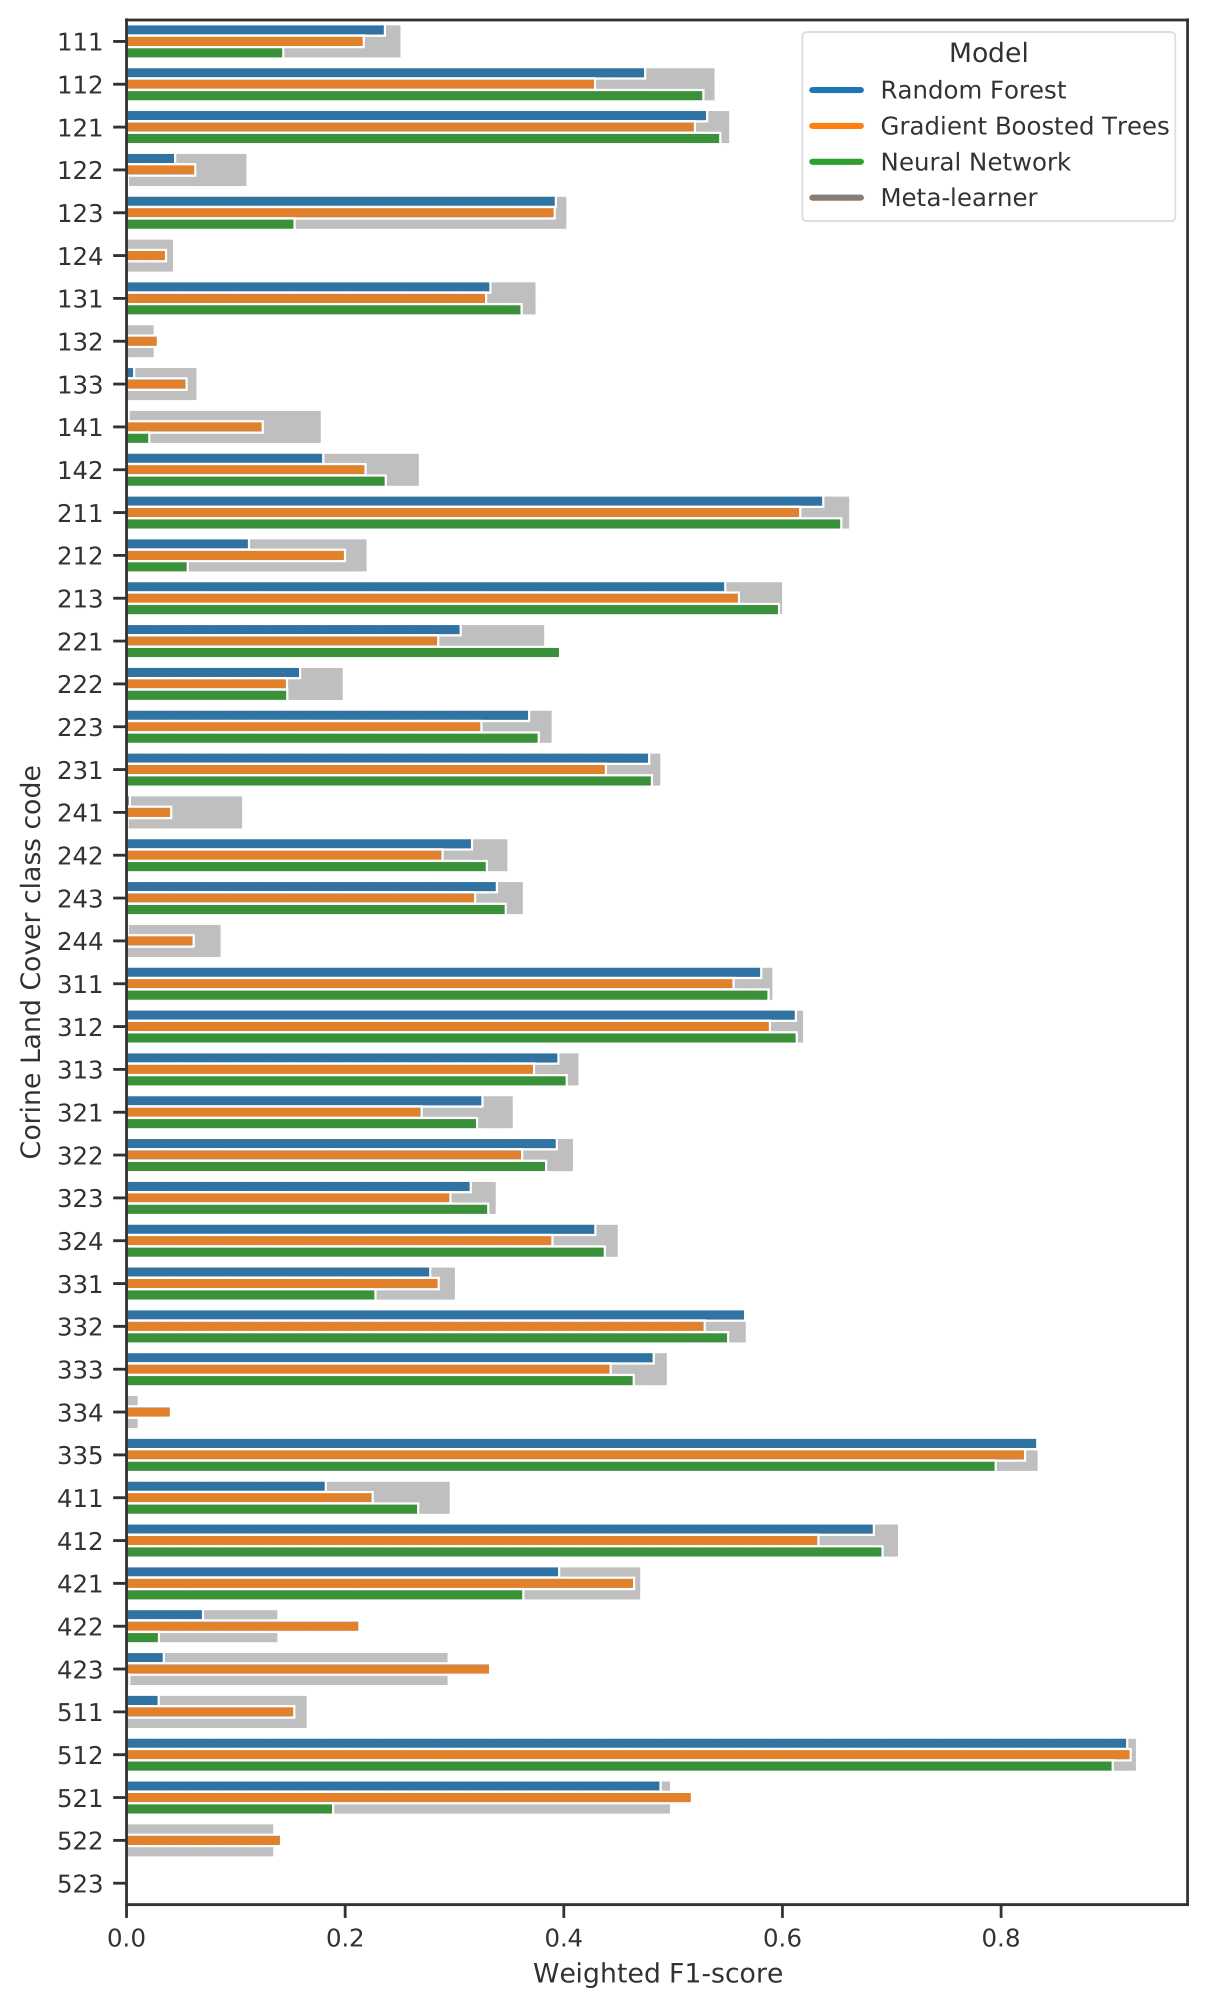
\includegraphics[width=0.8\linewidth]{figs_03/results_ensemble_comparison.png}
        \caption{Grouped bar plot of the F1-scores CLC class, plotted separately per model of the ensemble. Meta-learner performance is indicated in red on the background of each bar. If the random forest (blue), gradient boosted trees (orange) or neural network (green) outperformed the meta-learner, its bar will exceed the bigger meta-learner bar, indicating that the meta-learner did not learn to incorporate the model's higher performance into its final prediction.}
        \label{fig:ensemble_comparison}
        \end{figure}
    
\subsection*{Time-series analysis results}
    %\emph{Edited by: Chris van Diemen and Martijn Witjes}

    Our NDVI slope maps show which areas have an increase or decrease in NDVI over time.  We selected 19500 LUCAS points that experienced LULC\@~change and overlaid these with our NDVI slope values.  Figs.\@~\ref{fig:copernicus_vs_ndvi}\@~and\@~\ref{fig:ndvi_detail} show clear differences in NDVI trend between LUCAS points that have undergone different LULC change processes.
    
    We generated annual maps for change classes (see Fig.\@~\ref{fig:landcover} for the maps of 2000 and 2019). Filtered data as well as the removed noise can be viewed from the ODS-Europe viewer.
    
    Fig.\@~\ref{fig:ndvi_slope} demonstrates how trend analysis can be used to explore large-scale trends and pixel-level details.
    
    \begin{figure}[hbt]
        \centering
        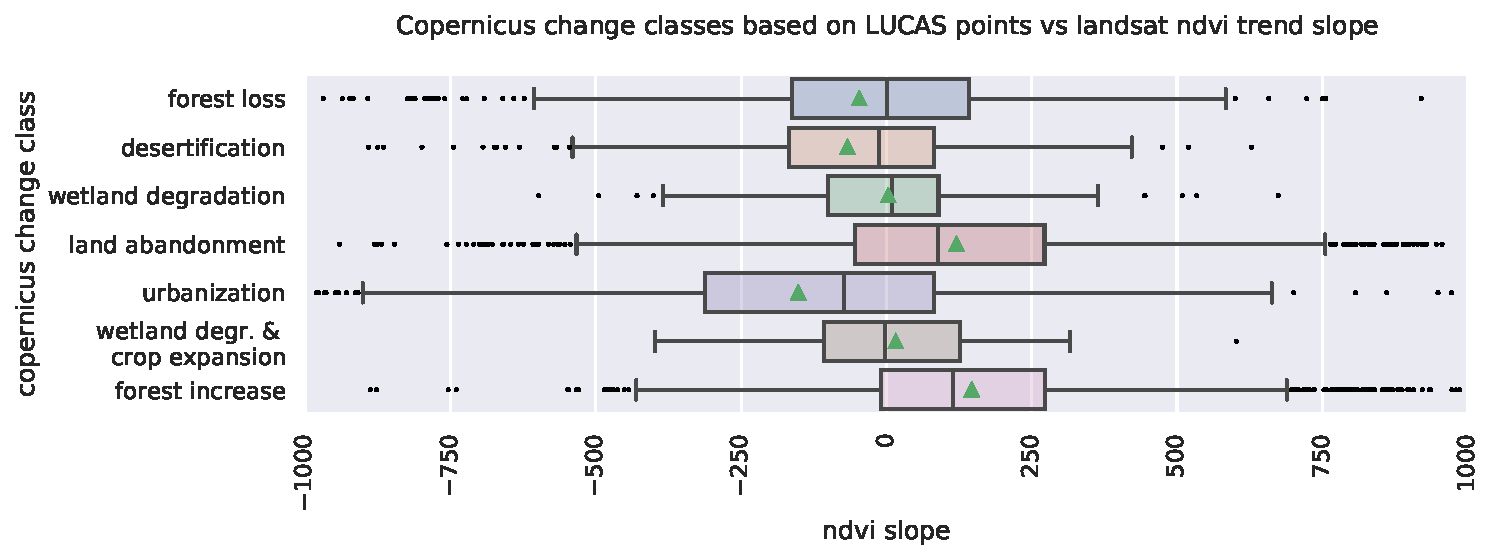
\includegraphics[width=\textwidth]{figs_03/results_cop_change_class_vs_ndvi_slopes.pdf}
        \caption{NDVI trend slope values of LUCAS points with selected LULC change dynamics, categorized according to the Copernicus change classes. The mean NDVI trend value is indicated with green triangles.
        } \label{fig:copernicus_vs_ndvi}
        \end{figure}
    
    
    \begin{figure}[hbt]
    \centering
    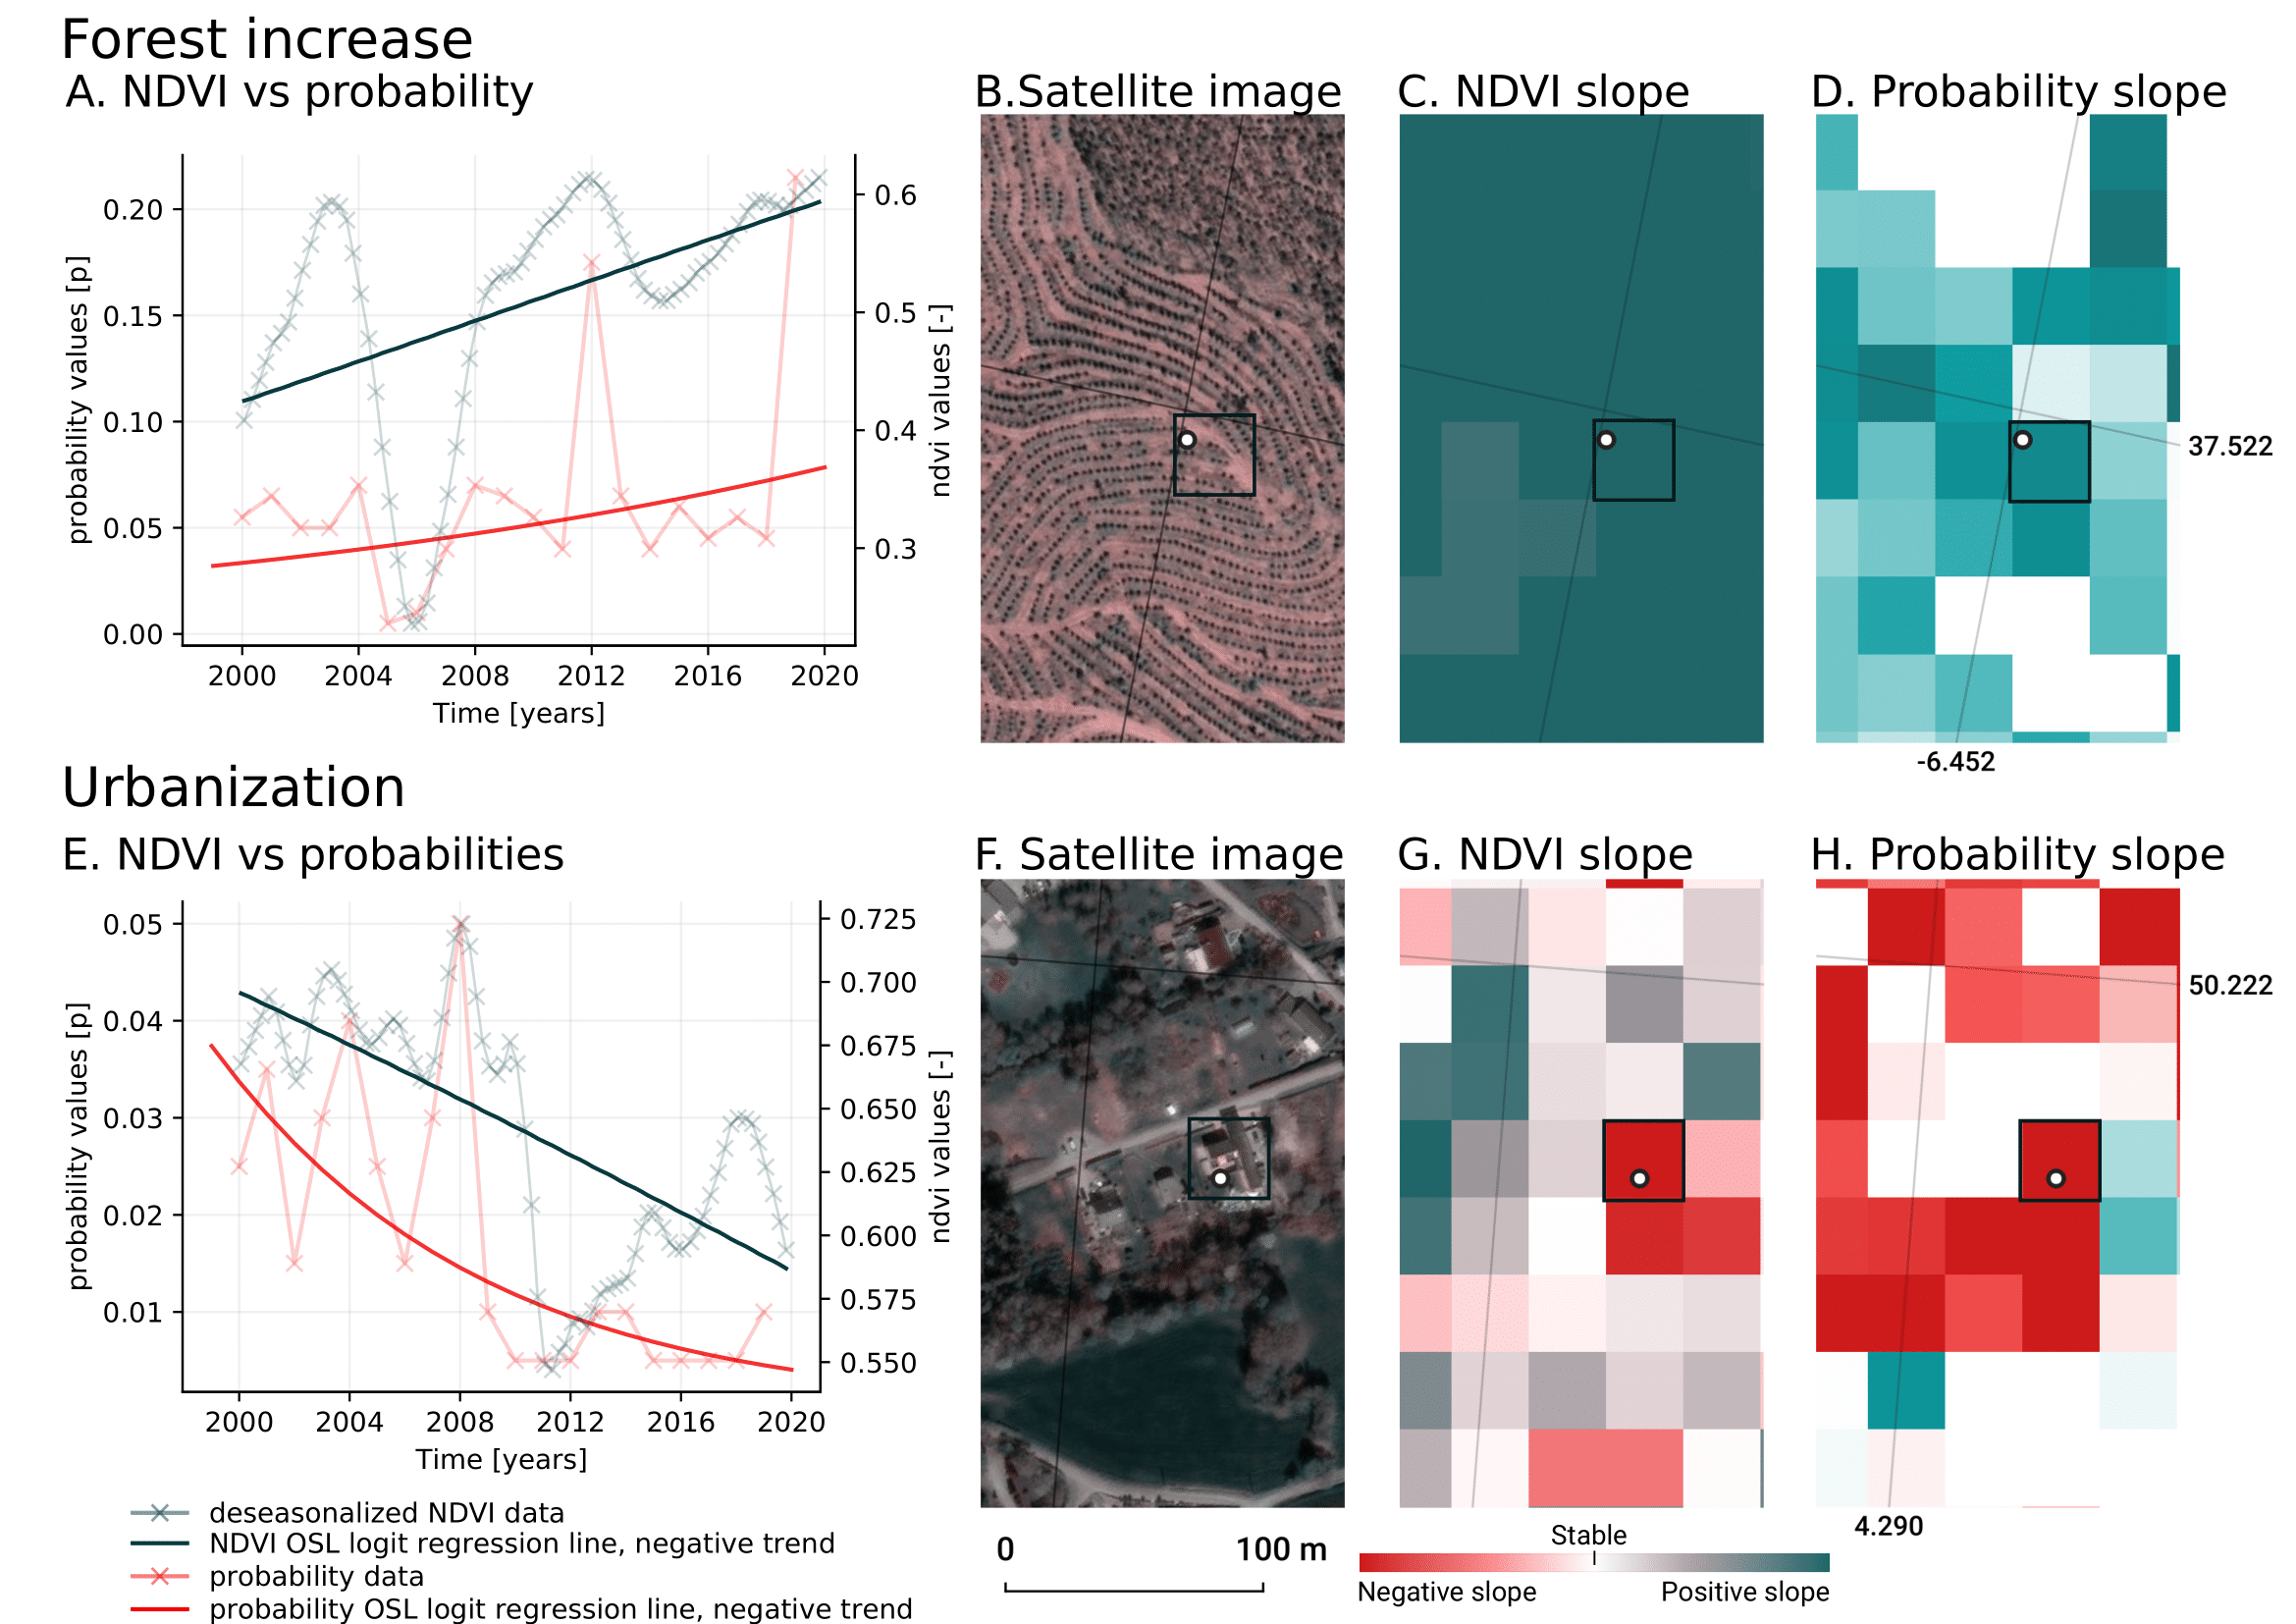
\includegraphics[width=\textwidth]{figs_03/results_ndvi_detail_plot.png}
    \caption{Detail plot of NDVI and LULC trends between 2000--2020 for 2 LUCAS points. NDVI trend is compared to forest increase (top) and urbanization (bottom). Left (A and E): A graph comparing the two trends, with green depicting de-seasonalized NDVI data and its trend, as calculated by logit OLS regression. Red depicts the annual probability values and associated trend of the compared LULC change classes (\emph{``312: Coniferous forest``} and \emph{``111: Continuous urban fabric``}, respectively). The maps, from left to right, depict the spatial context of the two points in (B/F) high-resolution satellite RGB, (C/G) slope of Landsat ARD NDVI trends, and (D/H) slope of LULC change class trends as predicted by our ensemble. The \emph{``in-situ``} observations of both points match the dynamic presented in the graph: Point 28681762 (top) experienced forest increase, while point 39143028 (bottom) is located in a recently constructed urban area.}

    \label{fig:ndvi_detail}
    \end{figure}
    
    Fig.\@~\ref{fig:ndvi_slope}-B1 and Fig.\@~\ref{fig:ndvi_slope}-B2 show areas of negative and positive slope occur adjacent to each other without gradual transitions. 
    Fig.\@~\ref{fig:ndvi_slope}-B3 and Fig.\@~\ref{fig:ndvi_slope}-B4 show examples of relatively large areas with homogeneous NDVI slope values. Overall, NDVI slopes in Europe tend to be positive, the largest exceptions being negative slope regions in Northern Scandinavia, Scotland, the Alps, South West France, Spain, Italy and Greece.
    
     The right-most subplots of Fig.\@~\ref{fig:ndvi_slope} show examples of where sudden land cover change classes at 30\texttimes30~m tend to match relatively large negative slopes, especially for change classes such as forest loss and urbanization.
    
    Fig. \@~\ref{fig:prominent_change} presents the long-term LULC change processes as suggested by our classification results. Fig.\@~\ref{fig:prominent_change}-A presents the dominant type of LULC change in a 5{\texttimes}5~km grid, while Fig.\@~\ref{fig:prominent_change}-B shows the intensity of change as part of the total area on a separate map using 20{\texttimes}20~km areas. Large parts of mainland Europe are characterized with reforestation as the main change with patches of urbanization scattered in between. Norway, Sweden and Finland are characterized with forest loss as the main LULC change class. Large areas in Spain have land abandonment and crop expansion as the main land use class. 
    When taking into account the intensity of the changes the central European countries seem to be stable with the Iberian peninsula, Scandinavia and parts of eastern Europe exhibiting more intense changes.
    
    \begin{figure}[!hp]
    % \vspace*{-1.5cm}
    % \hspace*{-3.5cm}
    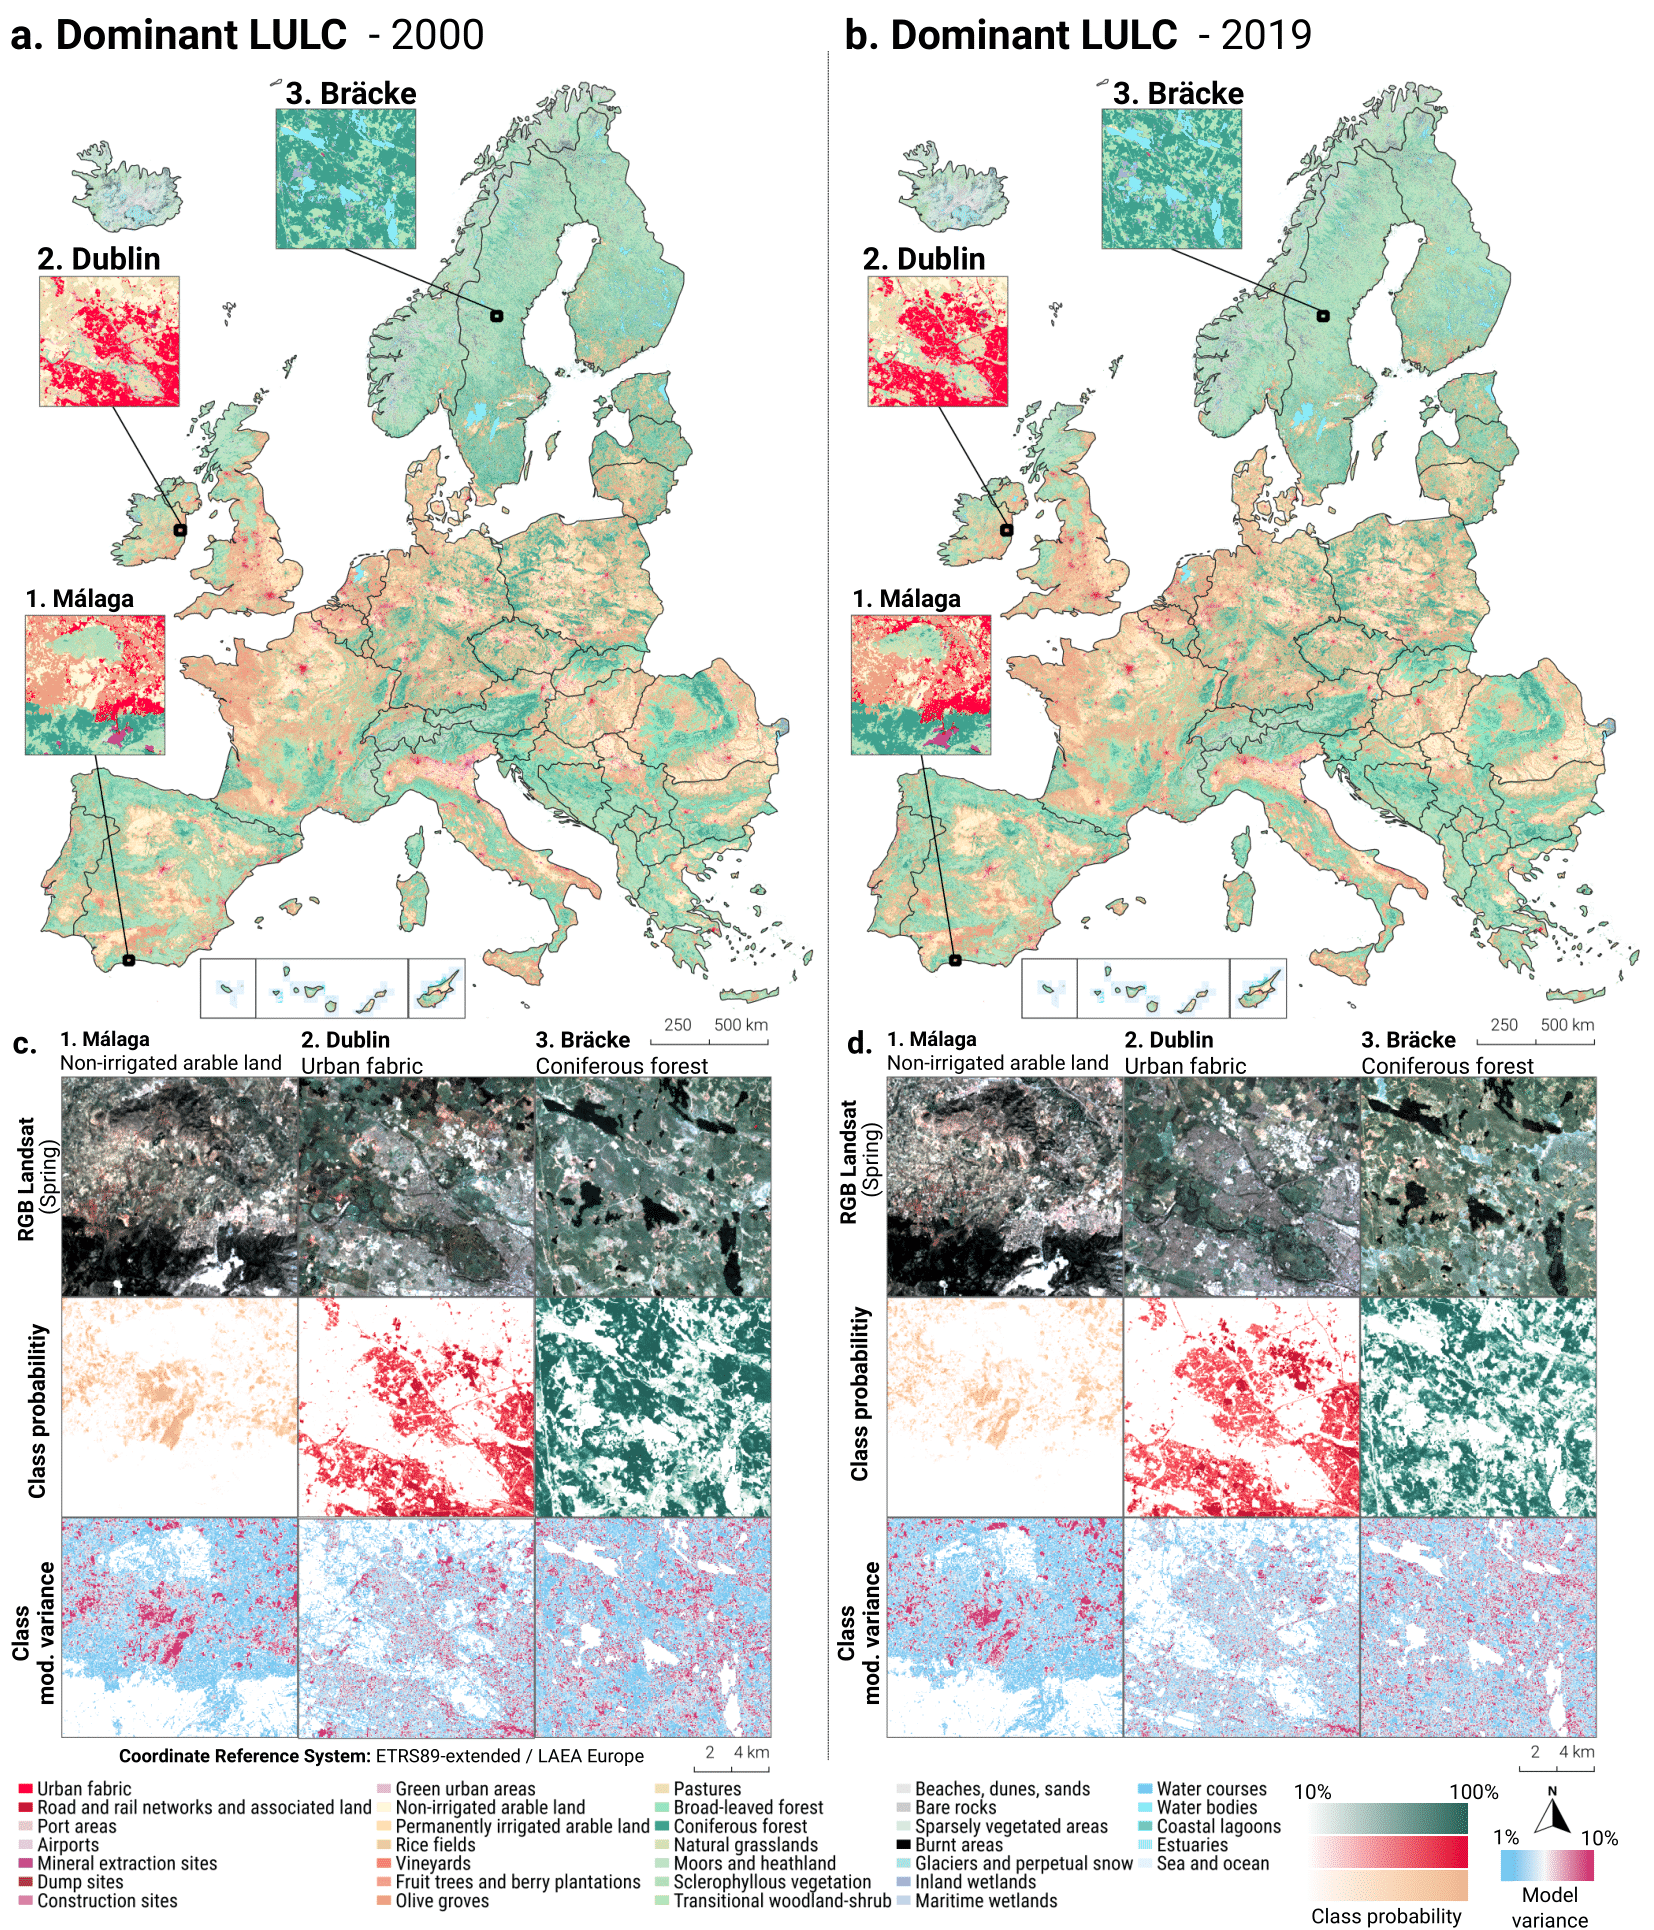
\includegraphics[width=1\textwidth]{figs_03/results_landcover.png}
    \caption{Dominant LULC classes, predicted probability and model variance for Non-irrigated arable land, Coniferous forest and Urban Fabric, RGB Landsat temporal composite (Spring season) for the years 2000 and 2019.}
    \label{fig:landcover}
    \end{figure}
    
    \begin{landscape}
    \begin{figure}[!hp]
    \vspace*{-1.5cm}
        \hspace*{-3.5cm}
    \centering 
    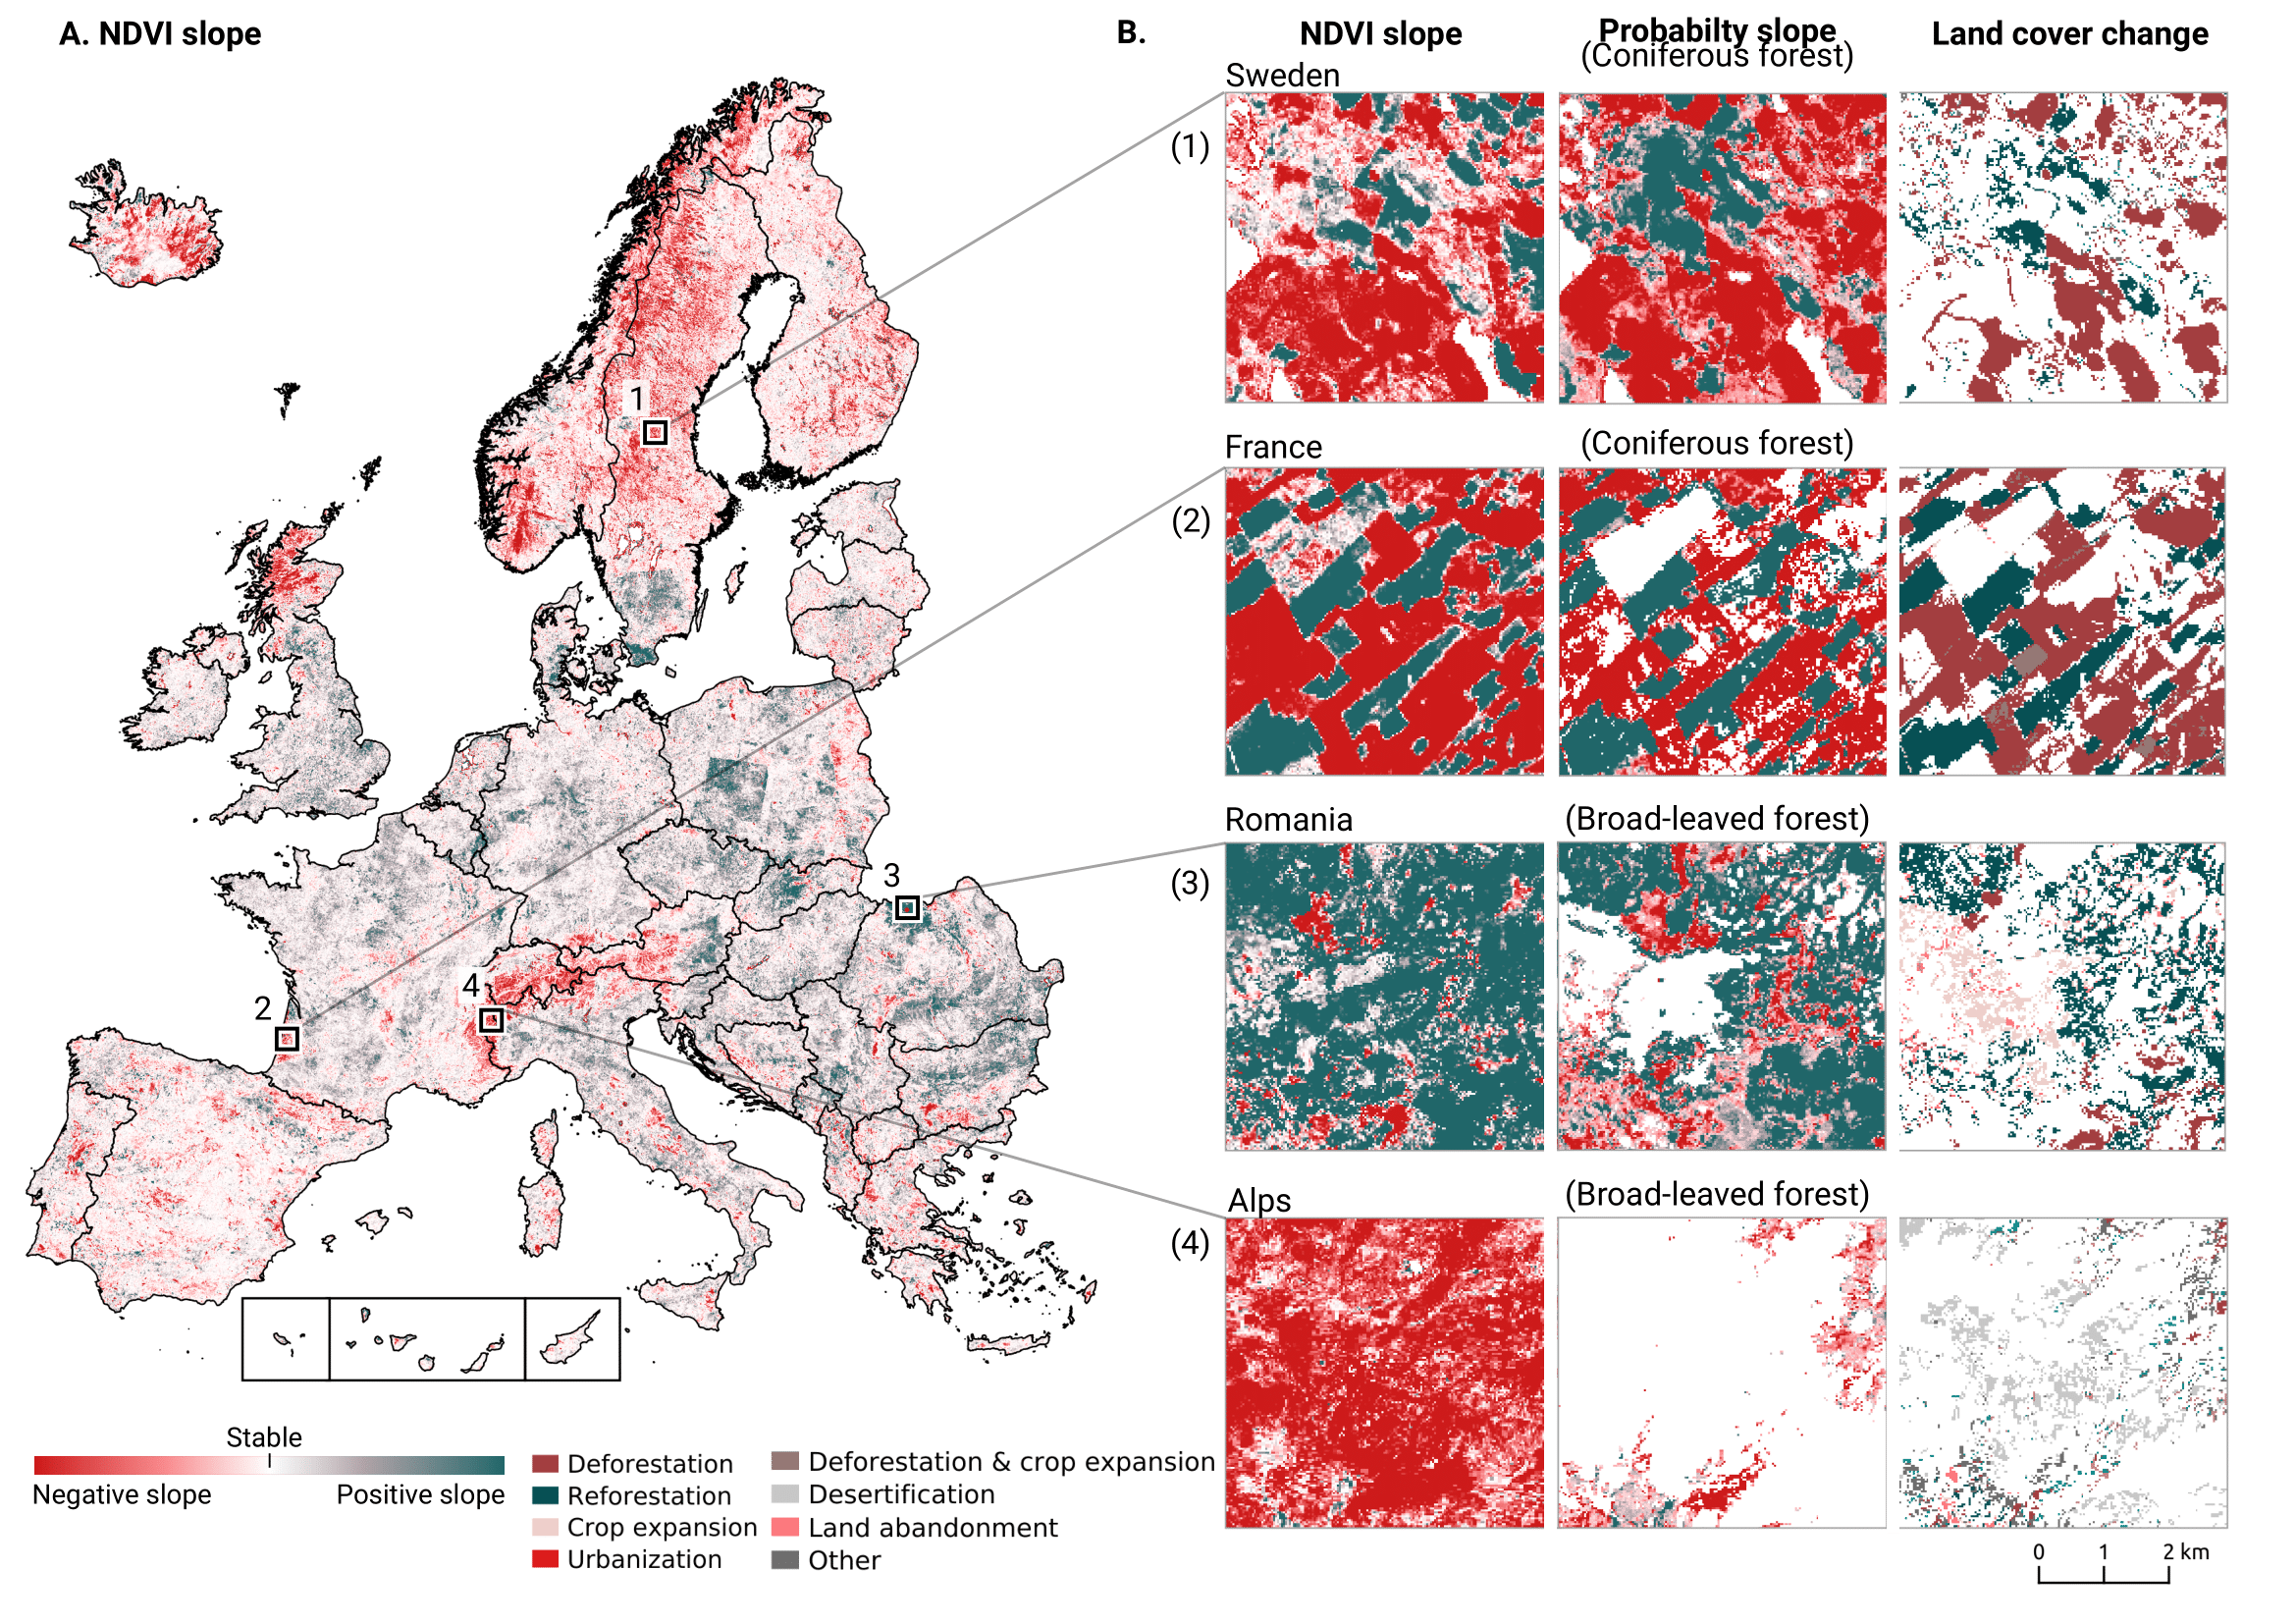
\includegraphics[width=1\textwidth]{figs_03/results_ndvi_visual.png}
    \caption{Trends in NDVI values between 2000 and 2019 compared to trends in LULC probabilities predicted by our ensemble model, as well as the derived LULC change classes between 2001 and 2018.} \label{fig:ndvi_slope}
    \end{figure}
    \end{landscape}
    
    \begin{landscape}
    \begin{figure}[!hp] 
    \centering 
    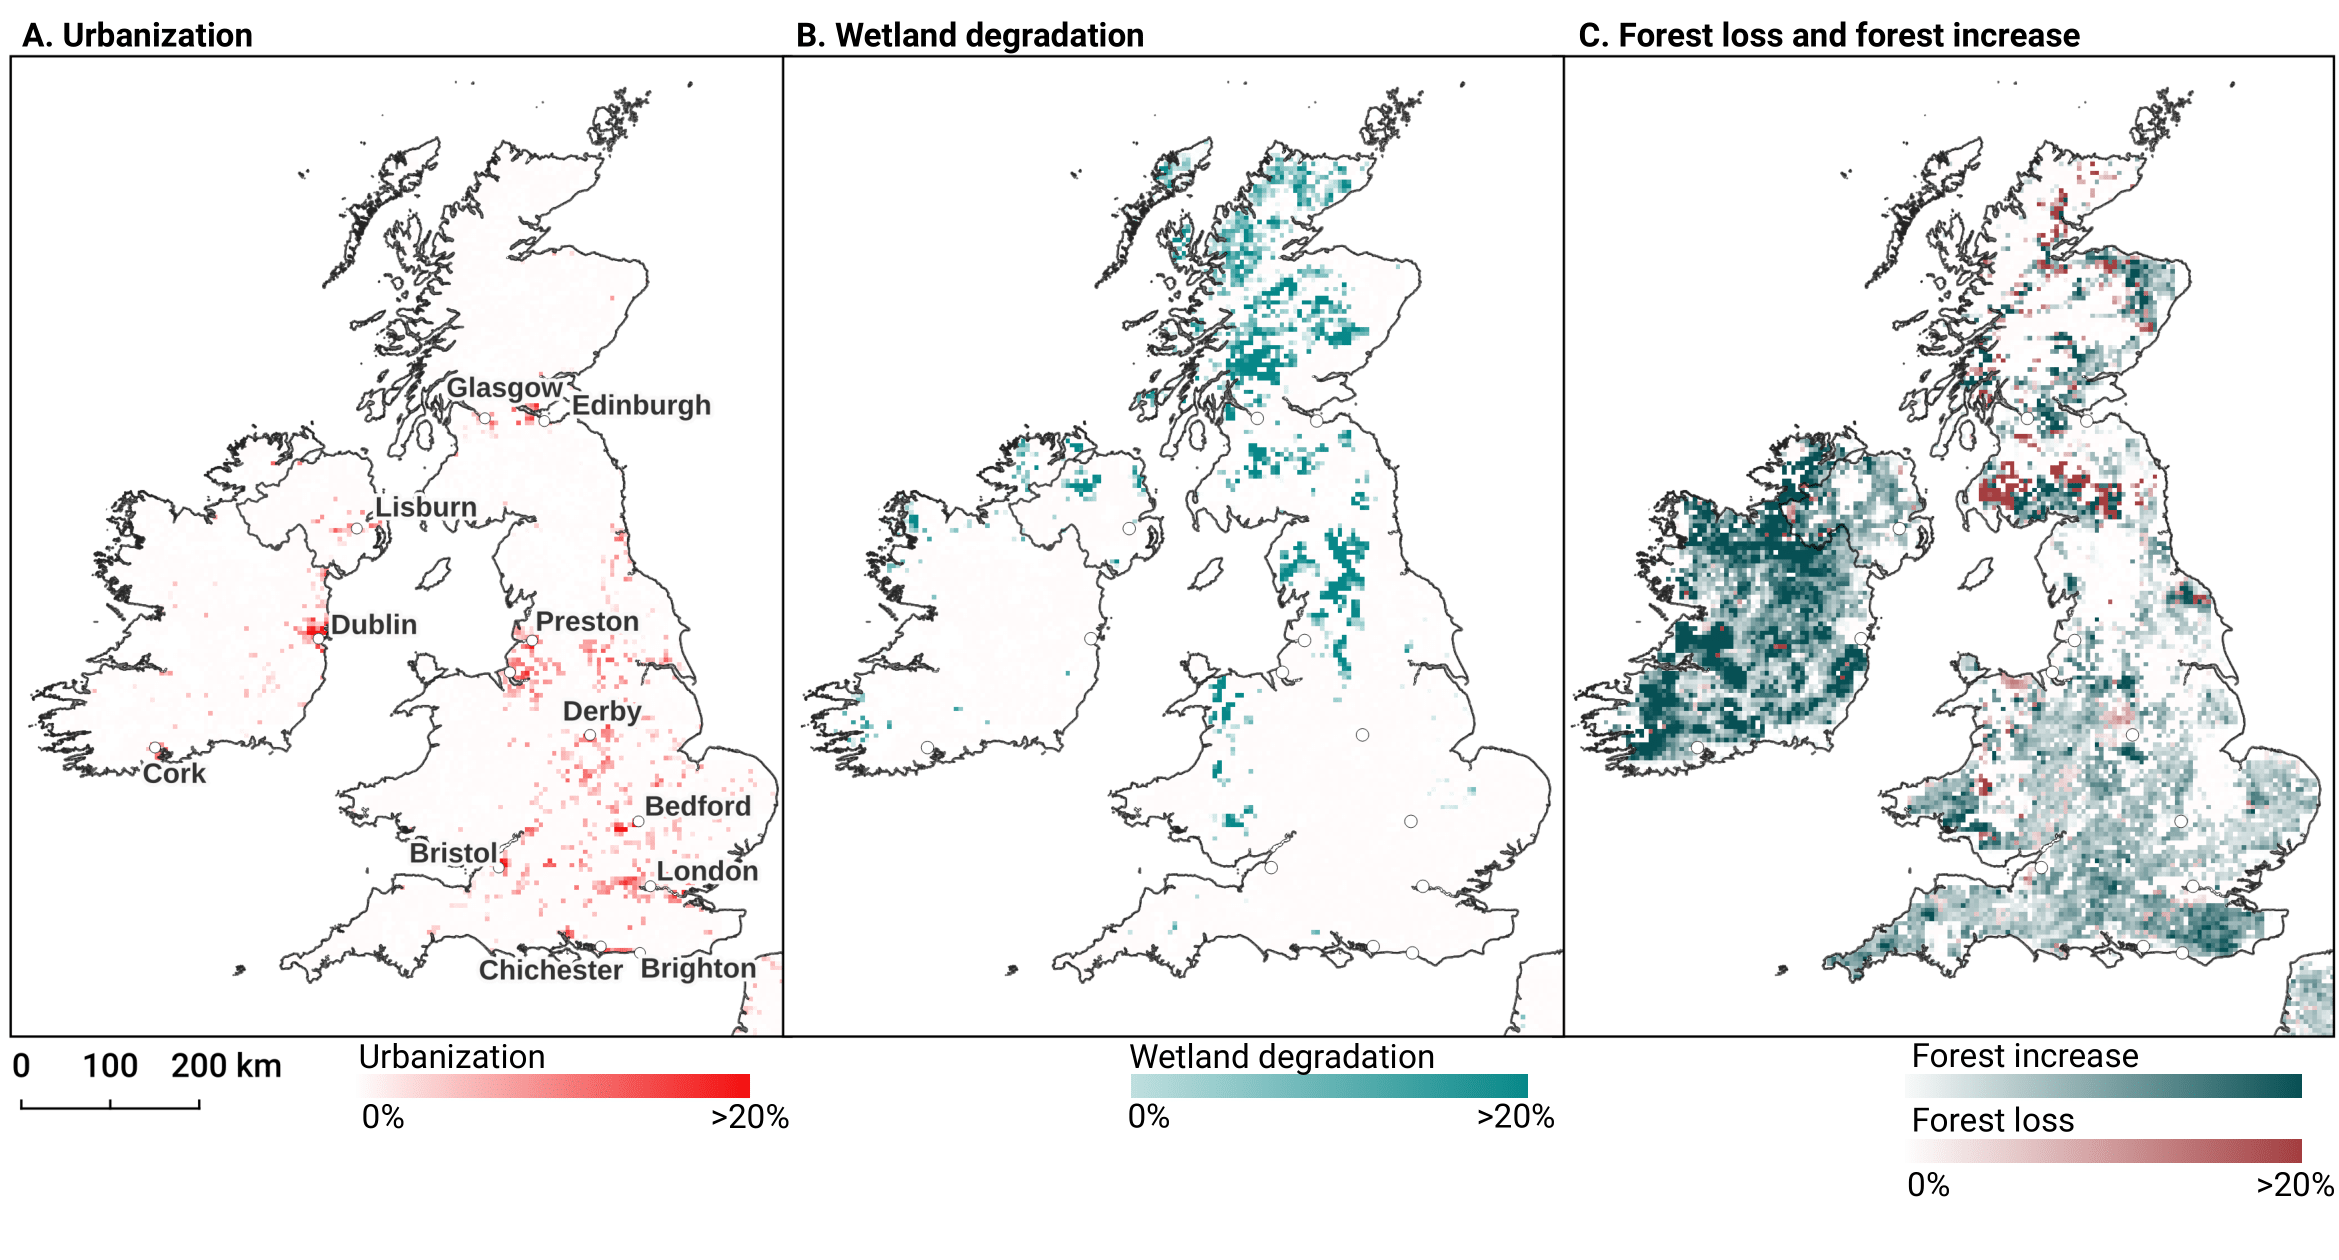
\includegraphics[width=1.3\textwidth]{figs_03/results_prevalent_change.png}
    \caption{Prevalent LULC change and change intensity on the British isles aggregated to 5{\texttimes}5km tiles, for three dynamics: Urbanization (A), Wetland degradation (B), and forest increase/decrease (C).} \label{fig:prominent_change}
    \end{figure}
    \end{landscape}

\section{Discussion}


\begin{quote}
\emph{``The appropriateness and adequacy of the 10-class schema used to describe land cover in today's human-dominated world needs a serious rethink. What is the value of a 10~m (resolution) landcover map that cannot capture a grassland being turned into a solar farm?''}\par
\textbf{Mysore Doreswamy Madhusudan}
\end{quote}

\subsection*{Summary findings}
    
We have presented a framework for automated prediction of land cover / land use classes and change analysis based on spatiotemporal Ensemble Machine Learning and per-pixel trend analysis. In this framework, we focused not only on predicting the most probable class, but also on mapping each probability and associated model variance. We believe that such detailed information gives a more holistic view of the land cover and land use and allows any future users to derive their own specialized maps of certain classes using probability thresholds and model variance per pixel and class, and/or to incorporate it in further spatial modeling. 

We show that in the context of reproducing the CLC legend, models trained on multi-year observations generalize better to unknown years than models trained on single-year observations, and that ensemble machine learning marginally outperforms single classifiers overall. Our accuracy assessment however indicates that several CLC classes remain hard to reproduce in the proposed workflow. The on-par performance on the S2GLC validation points, however, suggests that the framework is capable of generating accurate predictions for relatively detailed legends if they do not contain heterogeneous classes.
    
We further explained the time-series analysis framework for processing partial probabilities and NDVI values aiming at detection of significant spatiotemporal trends. We provide pixel-wise uncertainty measures (standard deviation of the slope / beta coefficient and R-square), which can also be used in any further spatial modeling. The whole framework, from hyper-parameter optimisation, fine-tuning, prediction and time-series analysis, is fully automated in the (\textsf{eumap} python package \url{https://eumap.readthedocs.io/}) and generates consistent results over time with quantified uncertainty, making it more cost-effective for future updates and additions.

\subsection*{Model performance}

Our spatial cross-validation accuracy assessment results indicate limited hard-class accuracy (Weighted F1-score of 0.494) at the highest classification level (43 classes) with several classes such as \emph{124: Airports''}, \emph{334: Burnt Areas} performing poorly, likely rendering them unfit for further use. However, a comparison of each class' separate log loss score indicates that the model predicted each class more accurately than the baseline. For example, \emph{522: Estuaries} was one of the least accurately predicted classes in the hard-class classification, but had a log loss ratio of 0.566. This means that probabilities were frequently correctly assigned to validation points in estuaries but overshadowed by other, more numerous classes (e.g. \emph{512: Water Bodies}), allowing a more accurate mapping of estuaries by adjusting the probability threshold for that specific class. Furthermore, our validation on the independent S2GLC dataset collected by \citet{malinowski2020} indicates that the accuracy of our model is comparable to the model used in their publication. Our conservative estimate (counting all points with predicted classes outside the S2GLC legend as errors) resulted in a weighted average F1-score of 0.854 and a kappa score of 0.794 and our optimistic estimate (where those points were removed before calculation) yielded F1: 0.889 and kappa: 0.867, while \citet{malinowski2020} reported 0.86 and 0.83, respectively. While these points were sampled to validate a 10\@~m resolution map and it is unclear how this affects the accuracy assessment, we could not find a reason to expect overestimated accuracy values in existing literature.
    
This suggests the nomenclature used by \citet{malinowski2020} is more optimized for remote sensing-based classification than the CLC legend and that the framework presented in this work is capable of achieving accuracy levels comparable to state-of-the-art 10~m resolution land cover products when using a more suitable legend. However, when we transformed our cross-validation results to the S2GLC legend, we obtained an F1-score of 0.611 and a kappa score of 0.535, which is considerably lower. This is unlikely to happen when comparing two datasets that are both sampled in a representative, proportional approach; it is therefore likely that the mismatch is caused by the training points in the  ODSE-LULC dataset that were generated from CLC centroids. 
    
The average weighted F1-score per year was 0.489 with a standard deviation of 0.135, while the average weighted F1-score per tile was 0.463, with a standard deviation of 0.150. This means that our model was more consistent through time than through space. A possible explanation is the unequal distribution of training points derived from the CLC data; we did not sample this data based on how much area they cover, but instead on how many separate areas occur in the data. Regions of Europe and classes with smaller CLC polygons may be over-represented in the data. Fig.\@~\ref{fig:tiles_support_vs_v1} shows that there is a slight but significant correlation between the number of points and cross-validation F1-score. This suggests that improving the CLC sampling strategy may improve the spatial consistency of our model.

\subsection*{Advantages and limitations of combining CLC and LUCAS points}

We included LUCAS points in our dataset in order to base our modeling and predictions on a consistent and quality-controlled dataset. However, in this work we found that training spatiotemporal models on LUCAS points lead to lower classification accuracy estimates than when only using CLC points (see Table\@~\ref{tab:spatial_vs_spatiotemporal_data_source}). This was unexpected, as LUCAS land cover information stems from actual ground observations, while the CLC points are pseudo-ground truth points from a dataset with a large minimum mapping unit. This suggests that either the LUCAS points are harder to reproduce with remote sensing techniques, or that the harmonization and data filtering process needs to be improved. Further testing is needed to clarify this.

\subsection*{Advantages and limitations of using spatiotemporal models}

The results of testing the generalization potential of spatiotemporal models with separate experiments (see methods and results sections about spatial vs spatiotemporal machine learning) show that spatiotemporal models generalize better to data from years they were not trained on. These findings suggest that we can use the existing model to predict land cover for 2020 and 2021 without collecting new training data: Preparing Landsat images for these periods would be likely enough.
    
Our results also suggests that we can use contemporary reference data to make consistent predictions for periods \textit{prior} to the year 2000, for which very little training data is available. We intend to produce predictions for the years 1995, 1990 and to 1985 in the next phase of our project. We did not do this previously because the Landsat ARD data \citep{potapov2020landsat} is only available after 1997. We need to compute and re-calibrate the Landsat 5, 6 and 7 products ourselves, which adds a higher level complexity due to the differences in sensors and acquisition plans.

What further limits us the fact that the long-term spatiotemporal approach aims at 30~m resolution data, while most current land cover products aim at a 10~m resolution. Furthermore, our approach is highly dependent on the availability of quality reference data from multiple years. Many continents except North America and Australia do not have access to datasets similar to LUCAS, which might become real challenge for applying the framework outside Europe, and especially in Africa, Latin America and Asia.
    
\subsection*{Advantages and limitations of using ensemble models}
    
We implemented ensemble machine learning in our framework for two main reasons. Firstly, to achieve the highest accuracy possible, and secondly, to allow for the inclusion of model variance as a proxy for the uncertainty of its predictions \citep{zhang2012ensemble}. Our results indicate that using an ensemble approach can indeed increase accuracy. Although the neural network component model scored a slightly higher weighted average F1-score than the meta-learner, the meta-learner achieved the highest F1-score on most classes, suggesting that the meta-learner sacrificed a slight amount of overall performance in order to improve performance on classes that the neural network could not recognize.
    
\begin{figure}[!hbt]
\centering
\includegraphics[width=\textwidth]{figs_03/discussion_model_variance.pdf}
\caption{Example of model variance (prediction uncertainty) in the city is of La Teste-de-Buch (France) for the class \emph{``Coniferous forest''}, visualized in the odse viewer (\url{https://maps.opendatascience.eu}): (a) model variance map with examples of two locations (P1 in 44{\textdegree}33'33.6"N 1{\textdegree}10'33.2"W; P2 in 44{\textdegree}32'11.8"N 1{\textdegree}02'38.0"W) with low and high variances, (b) probability values showing relatively high confidence, (c) original Landsat images RGB composite used for classification.} \label{fig:model_variance}
\end{figure}
    
Another advantage of doing ensembles with 5--fold CV with refitting of models and then stacking, is that we can generate maps of model variance (showing where multiple models have difficulties predicting probabilities). This allows users to identify problem areas (see Fig.\@~\ref{fig:model_variance}), determine where best to collect additional samples, or adjust their classification legend or probability thresholds. To our knowledge, mapping model error of predicted probabilities is a novel area and none of existing landcover datasets for EU provides such information on a per-pixel basis.



\subsection*{Time-series analysis, interpretations and challenges}
    %\emph{Edited by: Chris van Diemen and Martijn Witjes}
    
    
\citet{palahi2021concerns} found that the transition between Landsat 7 and 8 caused temporal inconsistency in the reflectance data. We tested whether these inconsistencies were propagated into our aggregated and harmonized dataset by calculating the NDVI values of 11~million pixels of our dataset. We then performed a two-sided t~test in order to analyze whether there was a difference in NDVI values before and after the launch of Landsat 8 in 2013 (see Fig.\@~\ref{fig:landsat_acquisition_vs_ndvi}). The t~test did not indicate a significant difference (test statistic of 0.0 and p=1.0) between the two distributions, suggesting that the inconsistencies from the transition were not propagated through our preprocessing step. 
    
The results of the probability trend analysis show some interesting patterns. We have focused on four geographic areas: (1) Sweden, as its forest dynamics have already garnered academic attention and it is an exemplary area where remote sensing techniques and on the ground measurements might come to different conclusions (see e.g.\@ \citet{ceccherini2020abrupt}). (2) South West France, as it is similar to the Sweden both in our data and is also compared by other authors \citep{senf2021mapping}. (3) Northern Romania because it shows a large region with positive trends for both NDVI and broad-leaved forest land cover, suggesting it is reforesting at high rates. Finally, we found large regions in the Alps (4) that show a strong negative trend for NDVI values that does not seem to correspond to a clear land use change. This signal in our data suggests there may be more artifacts and that further research is needed.
    
Forest loss in Europe is currently highly debated in academia \citep{senf2018canopy,ceccherini2020abrupt,senf2021mapping, palahi2021concerns, picard2021recent}. Discrepancies between national forest inventories and remote sensing techniques has led to disagreements in Sweden \citep{paulsson2020incorrect}, Finland \citep{korhonen2020new}, and Norway \citep{rossi2019assessing}. For instance, it was found that existing remote sensing products are deemed not fit for these types of analysis \citep{palahi2021concerns}. For these reasons, and because we do not validate our trend results, we neither attribute specific causes, nor do we analyze differences between specific time periods. 
    
Further comparison of the most prominent change between 2001--2018 and our results suggest that forest is disappearing more than it is re-appearing in multiple locations. This is corroborated by Global Forest Watch forest gain data; for example, the J\"{a}mtland region in Sweden lost 287k~ha of tree cover and gained 164k~ha between 2001 and 2012 \citep{hansen2013high}. We present the case of the Landes region in France here as well as it shows a similar pattern to large parts of Sweden and is a known area for large scale forest harvesting \citep{senf2021mapping}. These cases exemplify the usefulness of our maps for finding similar processes all over Europe by using a combination of the data that is presented here. More testing and ground-validation of the land cover changes is needed to assess which changes are over-estimations and which are realistic.
    
\begin{figure}[!hbt]
\centering
\hspace*{-1.5cm}
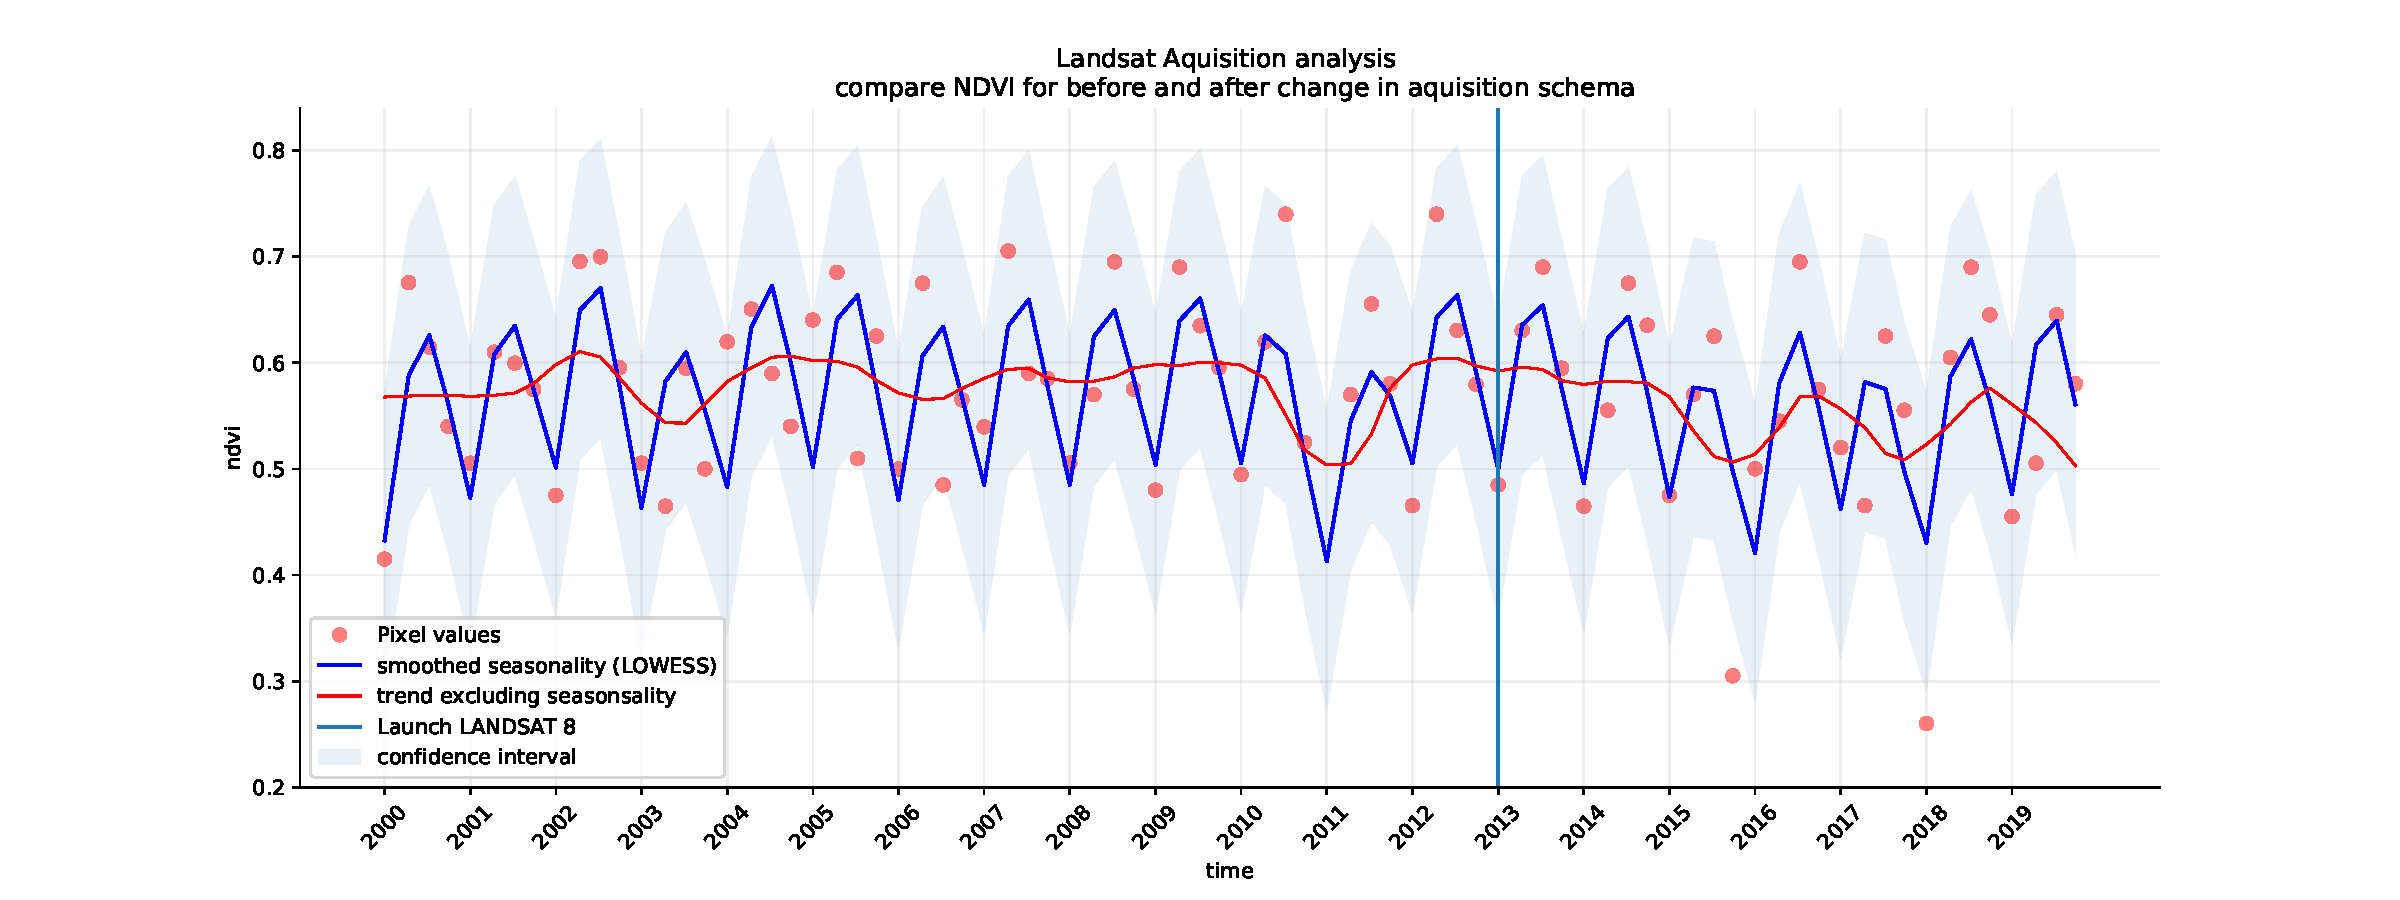
\includegraphics[width=1\textwidth]{figs_03/discussion_landsat_acquisition.pdf}
\caption{NDVI signal for 880 million pixel values in our Landsat data between 2000 and 2019. Red dots indicate the average for each season for 880 million pixels over 11 tiles. The vertical line indicates the launch of Landsat 8, after which the acquisition scheme changed. This sample suggests that the structural difference between the two acquisition schemes in the Landsat ARD product created by \citet{potapov2020landsat} were not propagated into our aggregated and harmonized dataset.} \label{fig:landsat_acquisition_vs_ndvi}
\end{figure}
        
Our data suggests that reforestation is the most prominent land cover change dynamic on a European scale. This change is accompanied by an observed increase of NDVI values. This observation is corroborated by the FAO's State of Europe’s Forests report 2020 which states that European forest cover has increased by 9\% between 1990 and 2020 \citep{rasi2020SoEF} and with global estimates that forest cover has increased by 7\% between 1982 and 2016 \citep{song2018global}. This increase is consistent with expectations that increased CO2 will enhance plant growth in general. Another concern that is raised is that most of the increase in forest gain is by planted forests \citep{payn2015changes} that are less valuable in terms of biodiversity and carbon sequestration \citep{liu2018tree} and less adaptable to climate change. One exemplary area with observed reforestation is found in Northern Romania in all parts of our time-series analysis: we see a change from grassland to forests making reforestation the dominant change class, the broad-leaved forest class probability is increasing, and NDVI values show positive trends. 
        
Finally, our data for the Alps shows unexpected negative NDVI trends for large parts of the Alps. This may be related to changes in snow cover as found by \citet{wang2018snow} in the Tibetan Plateau and by \citet{buus2006snow} in the Arctic regions. However, this is not corroborated by the probability slope for class \emph{``Glaciers and perpetual snow''} in our data. It is also possible that this is an artifact from our gap-filling step. Again, further study is necessary before any conclusions can be drawn.

\subsection*{Future work}
    
Even though our framework is comprehensive and has produced predictions of comparable accuracy to the current state-of-the-art on a less complex legend (see results section on S2GLC), after almost 14 months of processing the data and modeling land cover, we have found that that many aspects of our system could be improved:

\begin{itemize}
\item \emph{Improving performance without sacrificing detail}: We consider the poor performance on the 43-class level 3 CLC legend to be the main weakness of our approach. Including such a large and hierarchical legend theoretically makes the resulting data more useful to more potential users, but this will only manifest if the classifications are also reliable for research and policy. To this purpose, we will continue research on methods to improve classification performance while maintaining (or expanding) thematic resolution.

\item \emph{Cross-validation of land cover trends}: It was beyond the scope of our project to validate the results of our long-term trend analysis. Independently identifying and quantifying both sudden land cover changes (e.g. due to natural hazards such as fires and floods) and gradual dynamics such as urbanisation and vegetation succession. We have however published all our data online, enabling other research groups to test their usability for land monitoring projects.

\item \emph{Combining classification with Object-Based Image Analysis (OBIA) and pattern recognition}: Incorporating spatial context to our workflow could potentially improve performance for several classes that are defined by land use. For instance, class 124: \emph{``Airports''} was frequently misclassified as either urban fabric, non-irrigated arable land, pastures, or Sport and leisure facilities, another complex class that contains buildings and green areas. These predictions likely matched the land cover of the pixel, but missed the spatial patterns that make airports easily recognizable by humans (elongated landing paths). The same issue applies to most other artificial surface LULC classes. The relatively high importance of the TRI of the Landsat green band (see Fig.\@~\ref{fig:variable_importance}) suggests that additional feature engineering or other forms of incorporating the spatial context would improve classification performance on complex classes.
\end{itemize}

The field of land cover mapping is rapidly evolving. With exciting new global 10~m resolution products such as ESA WorldCover and Google's Dynamic World Map expected in 2021, we expect the LULC mapping bar to be raised quickly to higher resolution and higher accuracy. \citet{venter2021continentalscale} used low-cost infrastructure to produce land cover map of Europe at 10~m --- thanks to ESA and NASA making the majority of multispectral products publicly available, today everyone could potentially map the world's land cover from their laptop. \citet{szantoi2020addressing} show that many land cover products, however, are often ill-suited for practical actions or policy-making. As the quote at the start of this sections says \emph{``The appropriateness and adequacy of the 10-class schema used to describe land cover in today's human-dominated world needs a serious rethink''}, we assert that one should not look for land cover classification legends that are \emph{``low-laying fruits''} for the newest Sentinel imagery, but build people- and policy-oriented datasets that can directly help with spatial planning and land restoration. Our primary focus, thus, will remain on producing harmonised, complete, consistent, current and rapidly-updatable land cover maps that link to the past and allow for the unbiased estimation of long-term trends. We intend for this type of data to facilitate a better understanding of the key drivers of land degradation and restoration, so that we can help stakeholders on the ground make better decisions, and hopefully receive financial support for the ecosystem services our environment provides to us all.

\section{Conclusions} % (fold)

The spatiotemporal ensemble machine learning framework presented achieved a cross-validation weighted F1-score of 0.49, 0.63, and 0.83 when predicting 43 (level-3), 14 (level-2), and 5 classes (level-1). These values are lower than those reported by other current works that use classification systems with more optimized legends, and less classes. Our validation on an independent test dataset \citep{malinowski2020} with such an optimized legend yielded accuracy metrics comparable to  \citet{malinowski2020}. This indicates that the framework is capable of achieving similar performance to state-of-the-art methods, without any post-processing, and on a coarser spatial resolution, given a less ambitious task.

In our experiments, spatiotemporal models generalized better to EO data from previously unseen years: Spatiotemporal models outperformed spatial models on known-year classification by 2.7\% and unknown-year classification by 3.5\%. This suggests that spatiotemporal modeling, as incorporated in the presented framework, can be used to predict LULC for years of which no LULC observations exist, even prior to 2000 and beyond 2020.

Other methodological advantages of using spatiotemporal ML are (1) that it helps produce harmonized predictions over the span of years, (2) that the fitted model can be used to predict LULC in years that were not included in its training dataset, allowing generalization to past and future periods, e.g.\@ to predict LULC for years prior to 2000 and beyond 2020. Also, it is an inherently simple system with whole land cover of EU represented basically with a single ensemble ML (a single file). The disadvantages of using spatiotemporal ML is that it requires enough training points spread through time, and EO data needs to be harmonized and gap-filled for the time-period of interest (in this case 2000--2019).

Time-series analysis of predicted LULC probabilities and harmonized NDVI images over continental Europe suggests forest loss in large parts of Sweden, the Alps, and Scotland. The Landsat ARD NDVI trend analysis in general matches the land degradation / reforestation classes with urbanization resulting in the biggest decrease of NDVI in Europe.
	\chapter[Iterative Mapping of Probabilities]{Iterative Mapping of Probabilities: A data fusion framework for generating accurate land cover maps that match area statistics}
\label{cha:chapter3}
\vspace*{\fill}
This chapter is based on:
\\
\\
% Full citation of the published (or submitted/in review) article
% This refers to the article key in the refs.bib file.
\fullcite{witjes2024iterative}
\newpage

\section*{Abstract}
% Core purpose
    Providing land cover estimates with both correct pixel-level class predictions and regional class area estimates is important for many monitoring and accounting purposes but rarely achieved by current land monitoring efforts. We propose a framework that uses class probabilities predicted by machine learning to guarantee that the mapped proportion of each class matches independent area estimates. 
    % Short methodology
    We used CatBoost models trained on CORINE data to predict probabilities for 8 primary LUCAS land cover classes in five European countries. We then used the proposed algorithm to produce proportional class maps that match Eurostat class area estimates. We validate these proportional class maps and baseline highest likelihood class maps with LUCAS land cover observations and S2GLC validation points.
    % Main findings
    Our results show that the framework and algorithms create maps that match area estimates, and that may also be more accurate than maps created with highest likelihood classification. This is especially the case with general-purpose models trained on data whose class proportions are not representative of the mapped area, which means that this algorithm can be used to localize such models for more accurate mapping of individual countries.

\newpage

\section{Introduction}
    % Why do we need area estimates and maps
    Land cover changes are fundamental to understanding the complex interplay between human activities and the environment \citep{winkler2021global}. Locating and quantifying this process is essential for several UN Sustainable Development Goals (SDG) \citep{unstats2023sdgs,romijn2016monitoring}, predicting and combating climate change \citep{unfccc2015adoption}, and preserving the diversity of life on earth \citep{cbd2016indicators}. For this, we currently rely on two main techniques: model-based mapping (pixel- or polygon based predictions) and design-based area estimation for a given region.
    
    % Area estimation from maps & its limitations
    Land cover maps enable visualization and analysis of spatial patterns, allowing the identification of drivers of change \citep{sy2019tropical}, quantifying carbon emissions \citep{avitabile2016carbon}, and targeted land management \citep{verburg2011challenges}. Design-based land area estimates, on the other hand, provide statistically-robust, model-free insights and estimates (typically with confidence intervals) of long-term trends and comparisons necessary for resource allocation, economic assessments, and international accountability \citep{olofsson2014good,gallego2017copernicus}. 
    As a result, policy and decision-makers often continue to rely on design-based area estimates, while there also is interest in maps that match the statistical area estimates. Due to the costs involved in performing such sampling surveys, there has long been a large interest in deriving area estimates directly from Earth Observation \citep{gallego2004remote}. Counting the number of pixels per class in the mapped area is the simplest method, but strongly discouraged due to unpredictable biases that may lead to over- and under-prediction of specific classes \citep{gallego2004remote,olofsson2014good,waldner2017where}. These area biases stem from many sources such as imbalanced training data \citep{he2009learning,mellor2015exploring,zhu2016optimizing}, the interaction between spatial resolution and pixel heterogeneity \citep{strahler2006global,herold2008challenges}, regional accuracy differences \citep{waldner2016towards,witjes2022spatiotemporal,duarte2023thematic}, and classifier design \citep{waldner2016towards,ghorbani2020comparing,demirkaya2020exploring}, and are therefore difficult to quantify in order to assess the uncertainty of predictions. 
    
    % Supplementing area estimates with mapping
    Unbiased area estimation based on pixel counting is possible using the confusion matrix computed from additional statistical reference data that are e.g. stratified according to the mapped classes. The map-based area estimates are then adjusted using commission and omission errors from according to the confusion matrix \citep{stehman2013estimating,stehman2014estimating,olofsson2013making,olofsson2014good}. 
    While it is not always feasible to obtain additional samples directly from the mapped area, many organizations still adhere to this approach as their standard practice. This is primarily because methods that rely on obtaining (additional) samples directly from the field tend to yield more precise area estimates compared to other methods \citep{finegold2016map,gallego2017copernicus,redd2022estimating,angelopoulos2023predictionpowered}.
    Recent developments suggest that unbiased area estimation may be possible without requiring post-classification sampling. For instance \citep{kleinewillinghofer2022unbiased} used Land Use/Cover Area Frame Survey (LUCAS) data and Copernicus High Resolution Layers (HRL) layers to show that it may be possible when the sampling design of the reference data is appropriate for the mapped phenomenon. Furthermore, \citet{sales2022land} derived area estimates from probabilities predicted by a random forest that were  more accurate than pixel counting in a binary classification context. Finally, the prediction-powered inference framework recently proposed by \citet{angelopoulos2023predictionpowered} makes it possible to derive quantity estimates with statistically valid confidence intervals that are smaller than those of purely sample-based estimates, without the need for post-classification sampling to adjust for model bias.
    
    % Use existing area estimates
    While these approaches show promise towards the end goal of deriving unbiased and accurate area estimates without requiring additional sampling, policy and decision makers continue to rely on sample-based area estimates such as the European Commission's LUCAS \citep{gallego2017copernicus}, and require maps that match their class proportions to enable localized interventions \citep{olofsson2014good}. Linking trends from area estimates to periodic maps would also facilitate temporally and spatially explicit assessment of land change, which is crucial for evaluating the impacts of critical human activities on the environment \citep{olofsson2014good,szantoi2020addressing,winkler2021global}. A key issue is that land cover monitoring from remote sensing data has been producing accurate spatial maps or providing "best" area estimates but rarely the focus has been on addressing both objectives together: an accurate map whose spatial distribution of classes is an exact match to those from a provided, trusted area estimate. This would effectively minimize both allocation and quantity disagreement \citep{pontius2011death}; pixel-wise classification errors and map-wide class quantities, respectively. Although this issue has been subject to study since the early years of remote sensing \citep{strahler1980use}, little research on related approaches has been presented so far. \citet{janssen1992knowledge} showed that using ancillary data about class area proportions can be used to improve classification accuracy, especially when there is uncertainty caused by 'mixed pixels' or difficulty separating classes in the feature space. \citet{mingguo2009effect} further analyzed such methods and showed that using prior probabilities to adjust classification thresholds can be used to change the balance of user's and producers's accuracy (precision and recall, respectively), but that this can cause small classes to disappear from the classified map. There have been few attempts to use ancillary data to go beyond improving per-pixel accuracy and actually making maps that match area estimates. A notable exception is the work done by \citet{troltzsch2009spatial} and \citet{brus2012statistical}, who made 1~km within-pixel tree species proportion maps of Europe, and used an iterative scaling and calibration technique to make them correspond to national forest statistics. 
    
    % Horvaths method
    More recently, \citet{horvath2021comparison} transformed predicted probability surfaces for vegetation types \citep{horvath2019distribution} into classified maps whose class distributions matched estimates derived from area frame survey data \citep{bryn2018land}, iterating over each species and assigning pixels on the map to that species until the expected prevalence was reached. However, they found that while their proposed methods produced maps with correct area proportions, these maps were less accurate than a map where each pixel was assigned to the class with the highest predicted probability, which suggests a trade-off between allocation and quantity disagreement. Furthermore, their proposed method left approximately 10\% of the map unclassified because not every pixel had probabilities for every class. 
    As soon as a pixel is assigned to one class, it can no longer be assigned to another; if pixels with probabilities above 0 for a certain class are rare, this leaves gaps in the classified map that must be filled with other methods.     
    We hypothesize that the amount of remaining unclassified pixels can be reduced by using 'smoother' input probability data. We consider such data 'smooth' when for each class, there are more pixels with a predicted probability value above zero than the number of required pixels on the final map. 
    This might be achieved by improving a model's ability to generalize such as using a bigger training dataset. This is often unfeasible in land cover classification due to the cost involved in collecting reference data, especially when area proportions must be correctly represented to obtain matching proportional predictions \citep{sales2022land,kleinewillinghofer2022unbiased}. \citet{horvath2021comparison} state that the accuracy of their proportional maps might be improved by using more accurately predicted input probabilities, and models trained on bigger training datasets tend to be more accurate \citep{myburgh2014impact,rodriguez-perez2017influence}. While there are general recommendations for training dataset size \citep{foody2006training,koshute2021recommending} and indications that tree-based methods can attain high accuracy without large training datasets \citep{ramezan2021effects} it is important to represent as much of the feature space as possible \citep{meyer2021predicting,wadoux2019sampling}. Furthermore, \citet{witjes2022spatiotemporal,witjes2023ecodatacube} showed that models trained on larger portions of CORINE-derived training data generalized better on unseen data, especially when mapping land cover in years not covered by the training dataset.
    
    % What are we doing in this paper
    This paper proposes and demonstrates a framework that employs predicted probabilities for land cover classes to create land cover maps that are both accurate and adhere to the class distribution determined by independent area estimates. We present an expanded version of the approach suggested by \citet{horvath2021comparison} that iterates over each class multiple times to minimize the overlap between classes: Iterative Mapping of Probabilities (IMP). We investigate the effectiveness and potential advantages of the proposed approach by answering the following research questions:
        
    \begin{enumerate}
    \item How does the quantity disagreement vary between proportional maps produced by IMP compare to that of highest likelihood class maps?
    \item How does the allocation disagreement vary between proportional maps and highest likelihood class maps?
    \item What is the impact of using machine learning models trained on national or larger area training datasets for producing proportional maps?
    \end{enumerate}

    We will answer these questions by creating proportional and highest likelihood class maps for five European countries. We will measure quantity disagreement by comparing the proportion of predicted classes to EuroStat area estimates, and allocation disagreement by validating the maps LUCAS land cover samples and S2GLC validation points. To assess the impact of using larger but less proportional training datasets, we do this twice: Once with a model trained on land cover data from the mapped country, and once with a model trained on a data from a group of countries.
        
\section{Materials and Methods}

    In this study, we classify land cover and produce maps that match area estimates by Eurostat across five neighboring European countries: Belgium, Czechia, Germany, Luxembourg, and The Netherlands. We utilized CORINE training points produced by \citep{witjes2022spatiotemporal}, from which we removed potential labeling errors using data from Copernicus HRL and OpenStreetMap. CatBoost classification models were then trained on these filtered points, with distinct models trained on subsets of the CORINE points from each country (referred to as \emph{local models}) and one \emph{general model} trained on CORINE points from all countries that adopted the LUCAS survey in 2006: Belgium, Czechia, France, Germany, Hungary, Italy, Luxembourg, The Netherlands, Poland, and Slovakia. For each of the five mapped countries, we predicted LUCAS land cover probabilities with the country's local model, as well as with the general model for the years 2009, 2012, 2015, 2017, and 2018. Each set of probabilities was used to create two hard-class land cover maps: One \emph{highest likelihood class map} created through highest likelihood classification, and one \emph{proportional class map}, created by the proposed algorithm in an attempt to match land cover class quantities with official LUCAS estimates. We validated our annual maps of 2009, 2012, 2015 and 2018 with the LUCAS points compiled by \citep{dandrimont2020harmonised}. The maps for 2017 were validated with a separate dataset that was explicitly created to validate the S2GLC land cover map of 2017 \citep{jenerowicz2021validation}. We used this evaluation to compare the classification performance of local and  general models, as well as highest likelihood class maps and proportional maps. An overview of our methodology is provided in Fig.~\ref{fig:workflow}.

    \begin{figure}
    \centering
    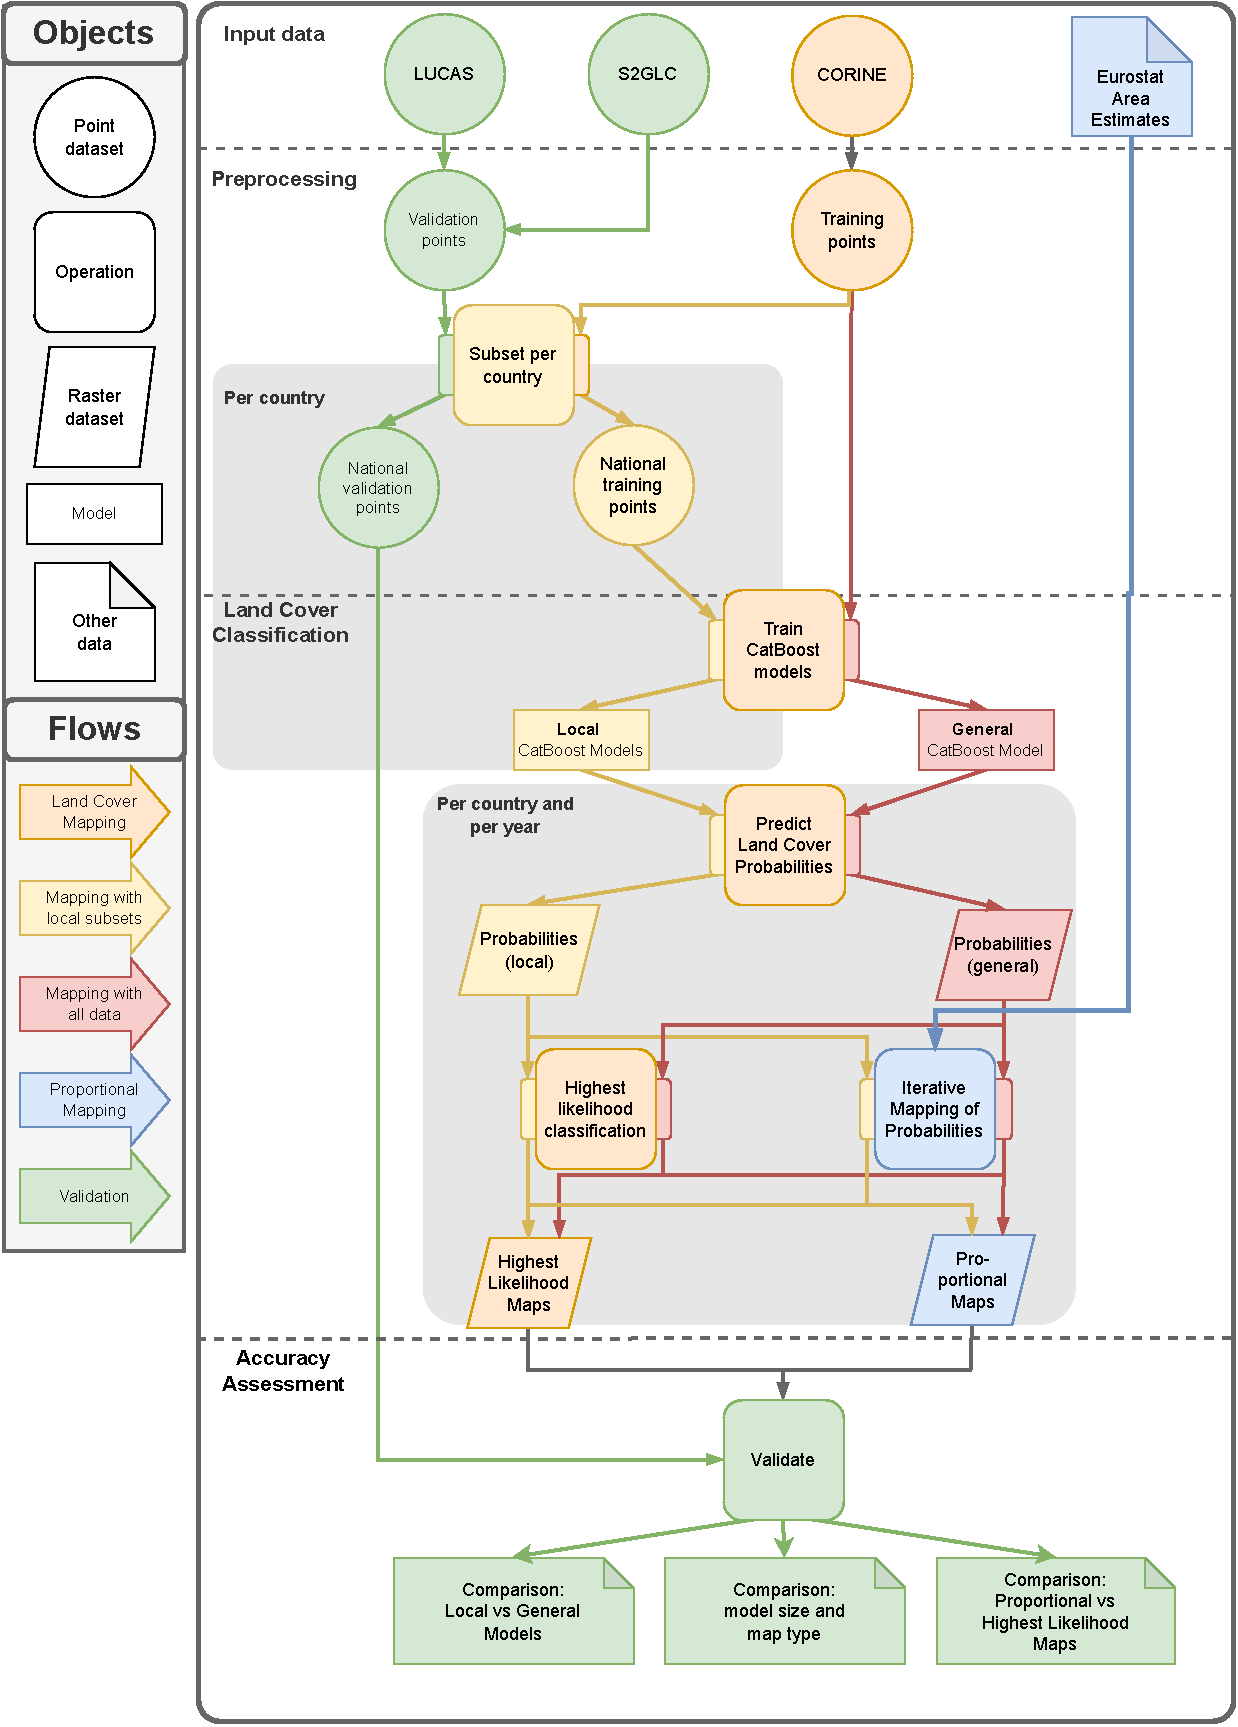
\includegraphics[width=\linewidth]{figs_04/fig1_methodology.pdf}
    % https://drive.google.com/file/d/1jB1FImQ1uke8RK1EKRSCaRF7iKUca4VG/view?usp=sharing
    \caption{Overview of the methodology to produce, validate, and compare highest likelihood and proportional maps. More detailed information on the production of the training data and features can be found in \citep{witjes2022spatiotemporal} and \citep{witjes2023ecodatacube}.}
    \label{fig:workflow}
    \end{figure}
    
    \subsection{Training and reference data}
    
        We used three different land cover point datasets for this study: 1) centroids of CORINE land cover polygons from 2006, 2012 and 2018 extracted by \citet{witjes2022spatiotemporal} (available on Zenodo \citep{landa2021multi}), 2) in-situ LUCAS samples of harmonized by \citet{dandrimont2020harmonised}, and 3) validation points of S2GLC land cover maps \citep{malinowski2020automated} produced by \citet{jenerowicz2021validation} (see Fig.~\ref{fig:points}). All classifiers were trained using CORINE centroids as reference, and all produced maps were validated on S2GLC and LUCAS samples. The strict sampling design and high accuracy of the LUCAS survey has made it a valuable resource in training and validating land cover models across Europe \citep{benevides2021land,pflugmacher2019mapping,sparks2022mapping,verhegghen2021accuracy,witjes2022spatiotemporal}, while S2GLC was specifically designed to validate land cover maps of Europe, using a stratified random sampling design to ensure proportional coverage of all European countries equal or larger in size than Luxembourg (see section 2.4 of \citet{malinowski2020automated}).

        \begin{figure}
        \centering
        \includegraphics[width=0.9\linewidth]{figs_04/fig2_points.pdf}
        
        \caption{Example of the distribution of CORINE training data \citep{witjes2022spatiotemporal}, LUCAS validation data \citep{dandrimont2020harmonised}, and S2GLC validation data \citep{jenerowicz2021validation}, each subset to the Netherlands to visualise their spatial distribution. Bottom right: An overview of countries and S2GLC validation sites surrounding the area of interest. Countries that were mapped and from which CORINE training data was extracted ("\textit{Mapped and trained}") are marked in dark gray, while countries from which additional CORINE points were extracted for the general model (\textit{"Trained"})are marked in light gray.}
        \label{fig:points}
        \end{figure}

    \subsubsection{Legend harmonization and filtering}
    
        We reclassified all CORINE-derived and S2GLC points to eight LUCAS land cover classes (level-1). In the case of CORINE points, we removed any points that belong to CORINE classes with no clear and exclusive match to a LUCAS class. This process was conducted according to the key shown in table \ref{tab:clc3_to_lucas1}

        Considering that the minimum mapping unit of CORINE is 25 hectares and the minimal width of mapped features 100m, CORINE polygons can encompass smaller-scale land cover types that differ from the main category of the polygon, introducing a risk of labeling errors. We counteracted this by screening the CORINE-derived points and removing all points whose land cover class were inconsistent with data from Copernicus HRL layers and OpenStreetMap in a similar way as the one detailed in \citet{witjes2022spatiotemporal}. For example, grassland training points were removed if Copernicus HRL layers indicated tree cover, or if OpenStreetMap rasters indicated roads or buildings were present at the points' coordinates. \ref{tab:corine_filtering} provides an overview of the data and conditions used to remove potentially faulty training points for each class.
    
        \begin{table}[H]
        \centering
        \caption{Reclassification key of CORINE and S2GLC land cover codes to LUCAS level 1 land cover. CORINE centroids of classes in the \textit{Not Used} category were removed from the training set.}
        \label{tab:clc3_to_lucas1}
        \begin{tabular}{lll}
        \hline
        LUCAS land cover & CORINE codes                             & S2GLC codes  \\ 
        \hline
        Artificial       & 111, 112, 121, 122, 132, 133             & 111          \\
        Cropland         & 211, 212, 213, 221, 222, 223, 241        & 211, 221     \\
        Woodland         & 311, 312, 313                            & 311, 312     \\
        Shrubland        & 322, 323, 324                            & 322          \\
        Grassland        & 231, 321                                 & 231          \\
        Bare land        & 331, 332, 333, 334, 335                  & 331, 335     \\
        Wetlands         & 411, 412, 421, 422, 423                  & 411, 412     \\
        Water            & 511, 512, 521, 522, 523                  & 511          \\ 
        \hline
        Not used         & 123, 124, 131, 141, 142, 242, 243, 244   &          \\
        \hline
        \end{tabular}
        \end{table} 


    \subsubsection{Feature space}
        All training points were overlaid on 224 covariates: Landsat data, derived spectral indices, a digital terrain model, and monthly minimum and maximum geometric temperature. 
        
        The Landsat data were originally published by \citet{potapov2020landsat}, aggregated to seasonal composites and gap-filled with a temporal moving window median (TMWM) algorithm by \citet{witjes2023ecodatacube}, and are openly available for download on \url{stac.ecodatacube.eu}. From the original bands (Blue, Green, Red, NIR, SWIR1, SWIR2, Thermal), several spectral indices were calculated: 
        \begin{enumerate}
            \item Normalized Difference Vegetation Index (NDVI) \citep{rouse1974monitoring}, 
            \item Soil Adjusted Vegetation Index (SAVI) \citep{huete1988soil}, 
            \item Modified Soil Adjusted Vegetation Index (MSAVI) \citep{qi1994modified}, 
            \item Normalized Difference Water Index (NDWI)  \citep{mcfeeters1996use}
            \item Normalized Difference Moisture Index(NDMI) \citep{gao1996ndwi},
            \item Normalized Burn Ratio (NBR) \citep{garcia1991mapping}, 
            \item Normalized Burn Ratio Plus (NBR+) \citep{alcaras2022normalized},
            \item Road Extraction Index (REI) \citep{shahi2015novel}, 
            \item Enhanced Vegetation Index (EVI) \citep{liu1995feedback}
        \end{enumerate}
        For each Landsat band and spectral index, the highest 25th percentile, median, and 75th percentile was included for each of the 4 seasons typical in Central Europe, resulting in 12 covariates for each of 7 bands and 8 indices, amounting to 192 Landsat-derived covariates.

        The digital terrain model was originally published by \citet{hengl2020continental}. We used 8 derived variables:
        \begin{enumerate}
            \item Slope percent
            \item Elevation (Lowest mode)
            \item Northness
            \item Easterness
            \item Positive openness \citep{yokoyama2002visualizing}
            \item Negative openness \citep{yokoyama2002visualizing}
            \item Multidirectional hillshade \citep{mark1992multidirectional}
            \item 315 degree sun azimuth hillshade \citep{mark1992multidirectional}
        \end{enumerate}
        
        The minimum and maximum geometric temperature is a geometric transformation of latitude and the day of the year \citep{kilibarda2014spatio}. Aggregated to monthly averages, this amounts to 24 covariates.

    \subsubsection{Area estimates}

        The area estimates used as input for the proposed algorithm, and to validate the quantity disagreement of all produced maps, were obtained from Eurostat \citep{eurostat_lucas}. This database reports how much of each LUCAS land cover class covers each country in each year that the LUCAS survey was performed: 2006, 2009, 2012, 2015, and 2018. We derived proxy area estimates for 2017 through linear interpolation of the area estimates of 2015 and 2018.
    
    \subsection{Machine learning}
    
        We trained CatBoost classifiers on the filtered and overlaid CORINE-derived points. CatBoost is an implementation of gradient boosting \citep{prokhorenkova2018catboost} that has seen much use in recent years due to its ability to achieve relatively high accuracy on large datasets in several fields \citep{hancock2020catboost}, notably being used to produce ESA WorldCover \citep{zanaga2022esa} and WorldCereal \citep{tricht2023worldcereal}. 
        
        %old= To study whether a larger feature space compensates for a class distribution that less closely matches the distributions of the target area, we created separate models trained only on samples from each country, as well as one model trained on samples from all countries that participated in the LUCAS program in 2006, resulting in five \textit{local} models and one \textit{general} model (see table \ref{tab:total_samples}).

        We trained six models in total: five \textit{local} models trained exclusively on CORINE training data from each country, and one \textit{general} model trained not only on data from the five countries, but also on CORINE data from all countries that participated in the LUCAS program in 2006. Each model was trained on CORINE data from all available years: 2006, 2012, and 2018. Table \ref{tab:total_samples} shows how many training points were used for the local models of each country, with the column \textit{Other} representing the countries from which training data was extracted, but which were not mapped by a local model (see also Fig. \ref{fig:points}). We included this general model in our analysis to investigate whether a larger feature space compensates for a less balanced class distribution.
        
        \begin{table}[H]
        \caption{Summary of CORINE points per country and LUCAS level 1 class, used to train the land cover models in this work. Local models were only trained on the available points for that country, while the general model was trained on all points, including those from other countries.}
        \label{tab:total_samples}
        \resizebox{\linewidth}{!}{%
        \begin{tabular}{lrrrrrrr}
        Lucas class & Belgium & Czechia & Germany & Luxembourg & Netherlands & Other   & Total \\
        \hline
        Woodland    & 13,661   & 46,555   & 202,657  & 1,575      & 4,934        & 683,623  & 953,005  \\
        Cropland    & 12,637   & 25,506   & 112,383  & 1,104      & 3,608        & 512,865  & 668,103  \\
        Grassland   & 10,176   & 21,923   & 69,541   & 689       & 2,647        & 255,673  & 354,649  \\
        Artificial  & 2,028    & 3,286    & 19,274   & 170       & 2,046        & 65,012   & 90,816   \\
        Shrubland   & 494     & 1,005    & 2,932    & 11        & 614         & 144,393  & 150,449  \\
        Water       & 451     & 1,994    & 8,415    & 20        & 1,222        & 25,085   & 37,187   \\
        Wetlands    & 50      & 272     & 2,903    & 3         & 584         & 8,385    & 12,197   \\
        Bare land   & 41      & 18      & 833     & 0         & 152         & 31,431   & 32,475   \\
        \hline
        Total       & 39,538   & 100,559  & 418,938  & 3,572      & 15,807       & 1,726,467 & 2,250,881 \\
        \hline
        \end{tabular}}
        \end{table}
    
        The training points were split up into 2996 30~km tiles. We randomly selected 5\% of these tiles as validation data. The remaining points were used to train all models. To prevent overfitting, we validated each model after each iteration on the points from the validation tiles. Training was automatically stopped when validation accuracy had not improved for 10 consecutive epochs, and the model resulting from the epoch where the most recent validation accuracy improvement was recorded was selected as the final model.
    
    \subsection{Land Cover Classification}
        For each country, we predicted probabilities for the eight LUCAS land cover classes in the years 2009, 2012, 2015, 2017 and 2018. We did this once with that country's local model, and once with general model. For each set of predicted probabilities, we created a \textit{highest probability class map} (HPC) by assigning each pixel to the class having the highest class probability. This resulted in ten highest probability class maps per country (five years,times two models).


    \subsection{Iterative Mapping of Probabilities}
    We implemented IMP, a post-processing algorithm, on each set of predicted probabilities (year, country, model). IMP is designed to create the most accurate possible hard-class map with 1) a given set of predicted probabilities and 2) an existing area estimate, based on the following assumptions: 
    \begin{enumerate}
        \item \textbf{Bias between classes} Models can have unknown biases and may overpredict certain classes by assigning relatively higher probabilities for them on average, which leads to rarer classes being underrepresented by highest likelihood classification \citep{he2009learning,waldner2017where}.
        \item \textbf{Ranking within classes} Within each class, the pixels with higher predicted values are more likely to correspond with actual occurrence of that class in a given pixel, regardless of the predicted probability values for other classes in the same pixel. Essentially, even if all probabilities for a single class are relatively low, they are at least roughly ranked in the correct order of likelihood for a given class. This is not always guaranteed \citep{niculescu2005predicting}, but can generally can be expected from accurate classifiers.
        \item \textbf{Overlap between classes:} When selecting pixels based on the level of their within-class relative probability, some pixels may be the best candidates for multiple classes (i.e. being in the top percentile of probabilities), either due to model bias, or due to multiple classes actually occurring inside the same pixel \citep{horvath2021comparison}.
    \end{enumerate}

    In general, IMP functions similar to the method proposed by \citet{horvath2021comparison}: It loops over every class, selecting the pixels with the highest predicted probability for that class and assigns the corresponding pixels on the output map to that class. However, to minimize the overlap problem, IMP does not do this once, but several times, each time selecting only the top percentile of available pixels for each class. We set the number of iterations to 20 in our presented experiments. This means that at every iteration, IMP selects the best 5\% of the target proportion from the best available pixels for each class.
    For example, a class which was estimated to cover 20\% of a country's surface, at the first iteration, only the pixels with 0.2\% of that class' highest predicted probabilities will be assigned to that class. At the second iteration, it would select and the pixels that are within 0.4\% of that range, but some of those pixels will have been assigned to other classes. Instead, it will select the pixels with the top 0.2\% highest probabilities for that class \textit{amongst the remaining unassigned pixels in the output map}. Figure~\ref{fig:imp} presents a visualisation of how IMP gradually fills a map until the proportions of each class matches those in the target area estimate. A detailed description of IMP is provided in \ref{alg:imp}.

    \begin{figure}[H]
        \centering
        % https://app.diagrams.net/#G1jB1FImQ1uke8RK1EKRSCaRF7iKUca4VG#%7B%22pageId%22%3A%22ZHYfUoFFE5HdqB9tgYix%22%7D
        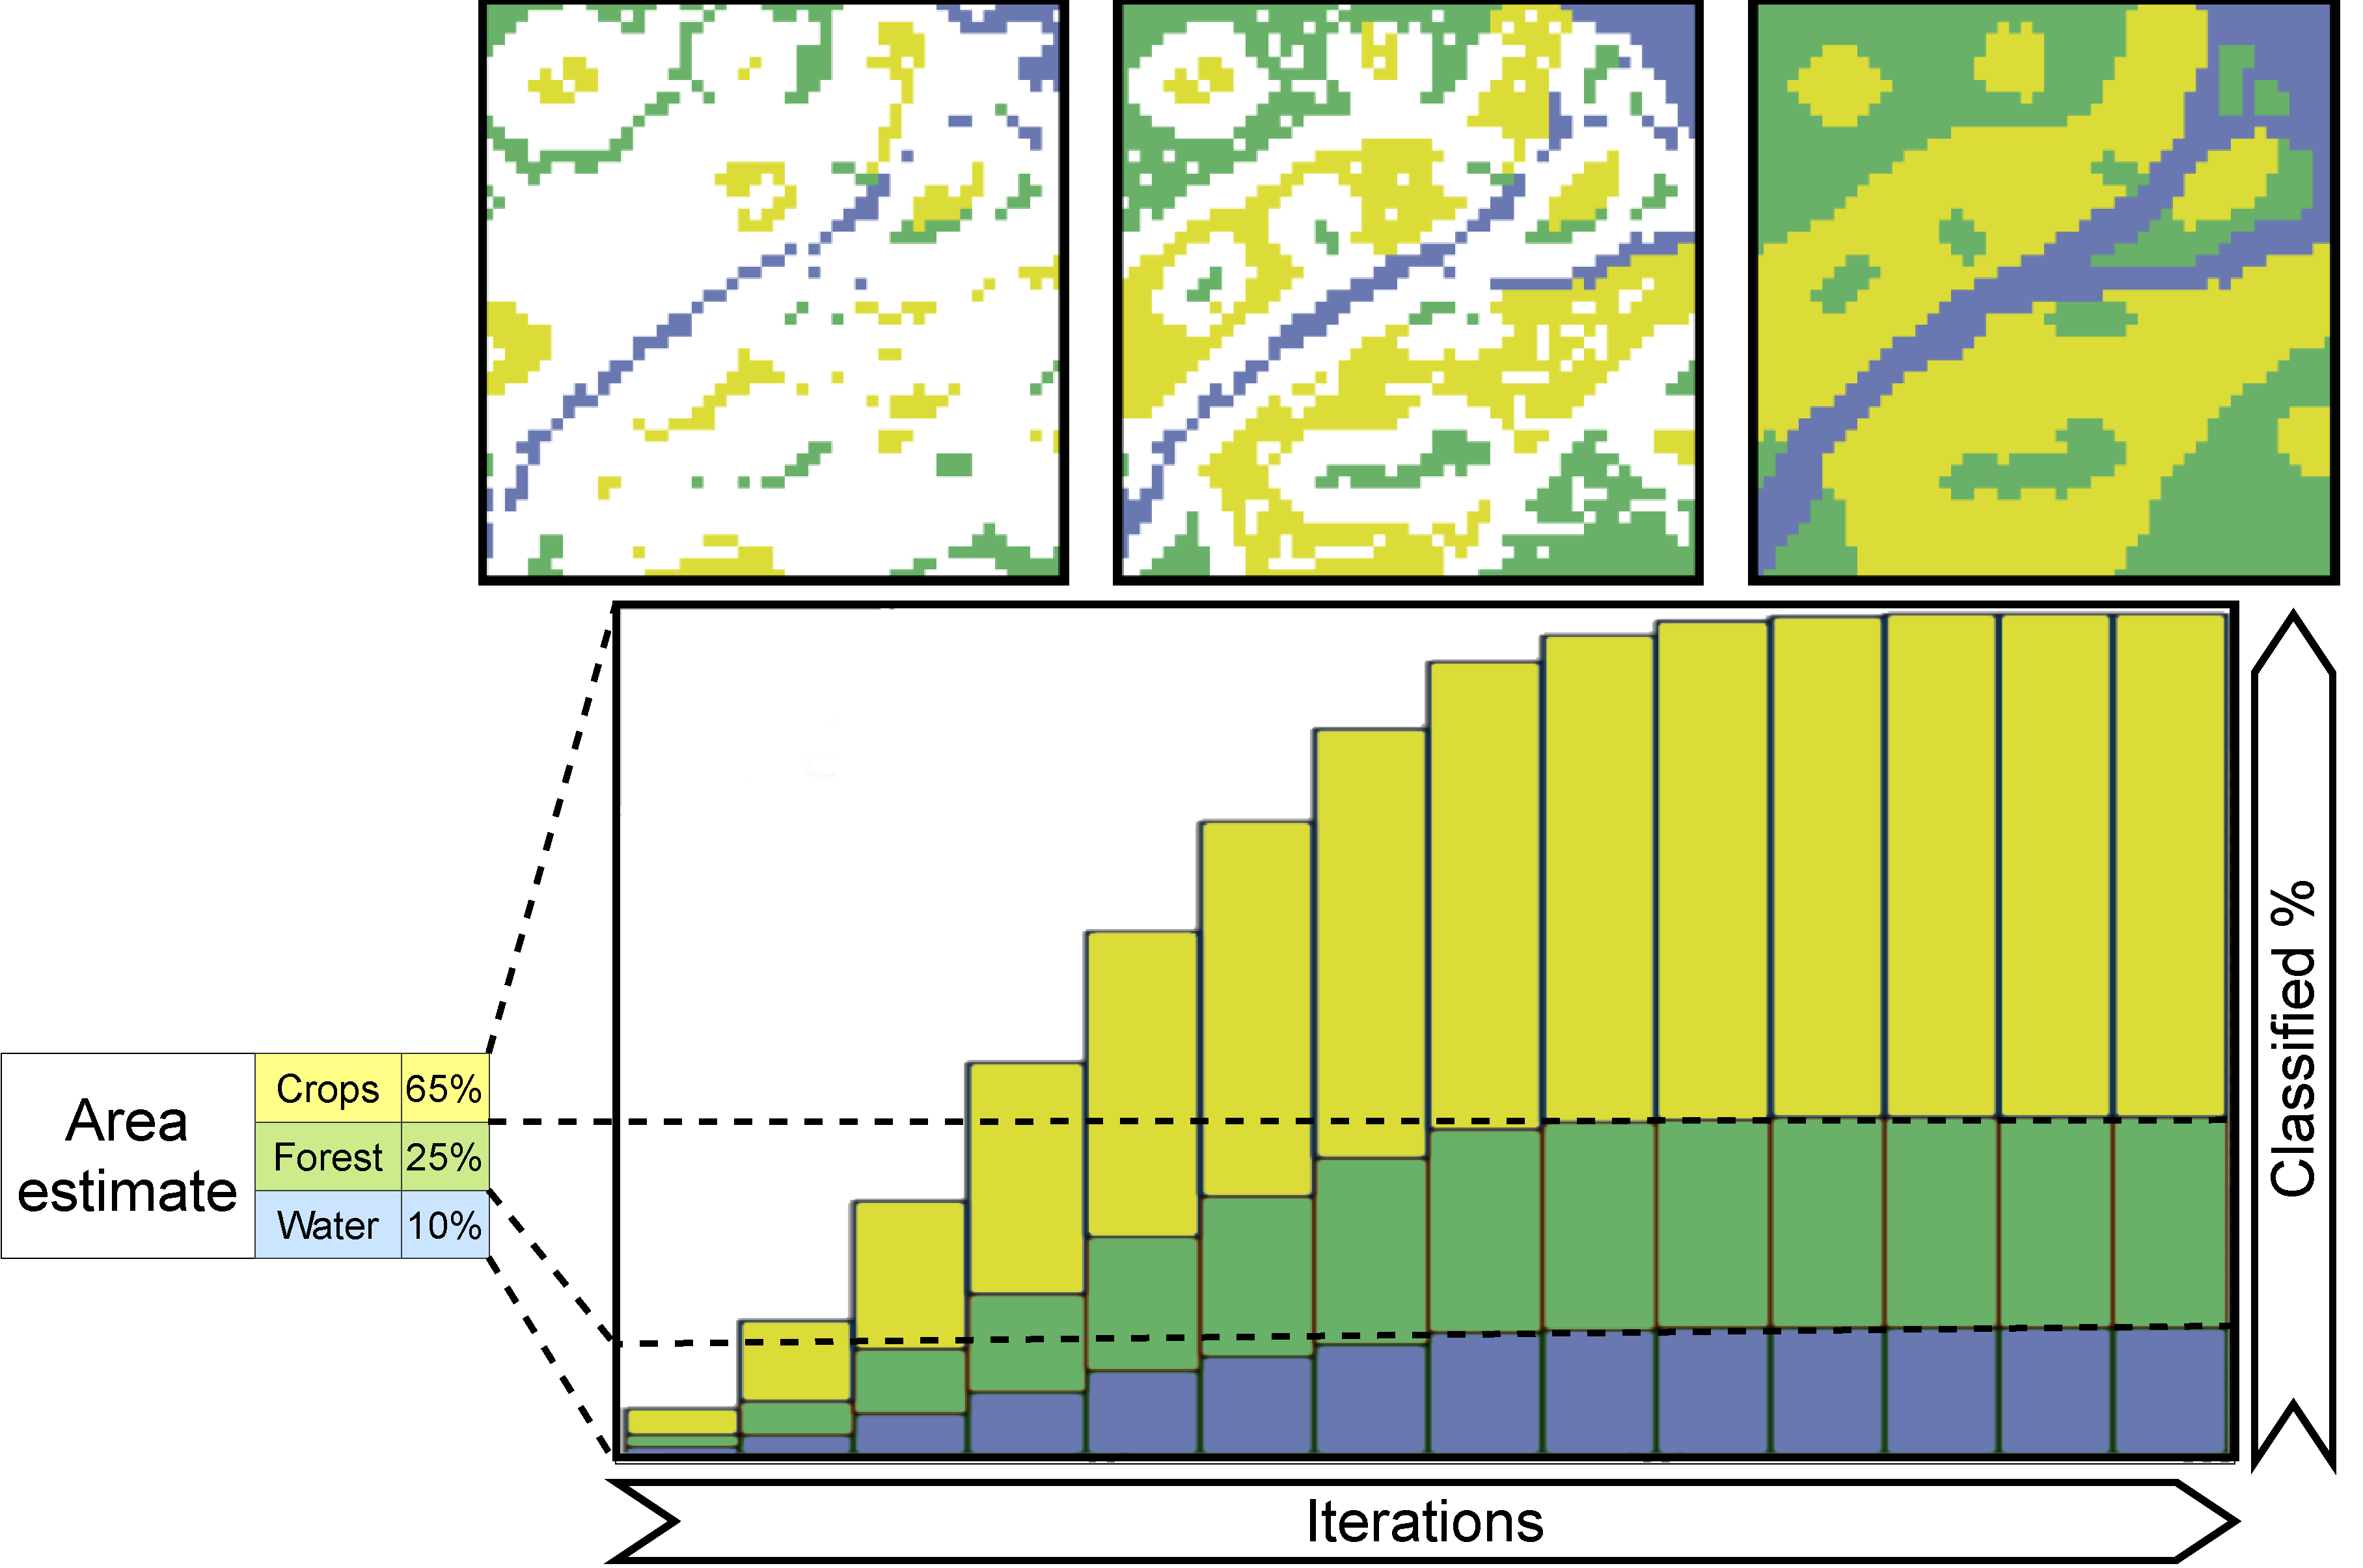
\includegraphics[width=0.9\textwidth]{figs_04/fig3_imp.pdf}
        \caption{Visualisation of how IMP gradually classifies each pixel in the study area, selecting the pixels with the highest available probabilities for each class in each iteration.}
        \label{fig:imp}
    \end{figure}

    \subsection{Accuracy Assessment}
    
    We assess the allocation and quantity disagreement \citep{pontius2011death} of the produced models and maps by validating the maps of 2009, 2012, 2015 and 2018 with LUCAS points \citep{dandrimont2020harmonised} and the maps of 2017 with S2GLC points \citep{jenerowicz2021validation}. Table~\ref{tab:total_lucas} shows the support per class per country for LUCAS points, and table~\ref{tab:total_s2glc} for the S2GLC points. We quantify allocation disagreement with the Weighted F1-score metric \citep{rijsbergen1980information}, a harmonic mean of user's and producer's accuracy (precision and recall), because it distinguishes classification performance more strictly on datasets with imbalanced class distributions. This makes it a useful metric to compare the classification performance when both accuracy and proportion of each class are important. This is done both for the \textit{highest likelihood} class maps (based on the highest probability per point or pixel) and the \textit{proportional} class maps produced by IMP. We measure quantity disagreement with the percentage that class-wise proportions of each map deviate from the area assessment of the target country in the target year.

    \begin{table}[H]
        \caption{Summary of LUCAS points per country and LUCAS level 1 class, used to validate the land cover maps of 2009, 2012, 2015, and 2018}
        \label{tab:total_lucas}
        \resizebox{\linewidth}{!}{%
        \begin{tabular}{lllllll}
        \toprule
        Lucas class & Belgium & Czechia & Germany & Luxembourg & Netherlands &   Total \\
        \midrule
         Artificial &   1,365 &   1,120 &   8,911 &         83 &       1,742 &  13,221 \\
           Cropland &   4,006 &  10,487 &  47,926 &        285 &       4,147 &  66,851 \\
           Woodland &   2,902 &   8,552 &  34,813 &        347 &       1,845 &  48,459 \\
          Shrubland &     139 &     218 &   1,042 &         15 &         271 &   1,685 \\
          Grassland &   4,332 &   6,199 &  30,540 &        402 &       6,014 &  47,487 \\
          Bare land &     236 &     306 &   1,332 &         13 &         286 &   2,173 \\
           Wetlands &     150 &     283 &   1,786 &          8 &         720 &   2,947 \\
              Water &      42 &      62 &     542 &          0 &         101 &     747 \\
              Total &  13,172 &  27,227 & 126,892 &      1,153 &      15,126 & 183,570 \\
        \bottomrule
        \end{tabular}}
    \end{table}

    \begin{table}[H]
        \caption{Summary of S2GLC points per country and LUCAS level 1 class, used to validate the land cover maps of 2017}
        \label{tab:total_s2glc}
        \resizebox{\linewidth}{!}{%
        \begin{tabular}{lrrrrrr}
        \toprule
        Lucas class & Belgium & Czechia & Germany & Luxembourg & Netherlands & Total \\
        \midrule
         Artificial &     115 &      39 &     183 &          8 &         193 &   538 \\
           Cropland &     325 &     439 &   1,211 &         16 &         246 & 2,237 \\
           Woodland &     225 &     258 &   1,039 &         23 &         202 & 1,747 \\
          Shrubland &       2 &       1 &       8 &          0 &          18 &    29 \\
          Grassland &     200 &      60 &     459 &         17 &         329 & 1,065 \\
          Bare land &      15 &      14 &      42 &          0 &          21 &    92 \\
           Wetlands &      12 &       6 &      10 &          0 &          49 &    77 \\
              Water &       2 &       0 &      23 &          0 &           7 &    32 \\
              Total &     896 &     817 &   2,975 &         64 &       1,065 & 5,817 \\
        \bottomrule
        \end{tabular}}
    \end{table}
    
\section{Results}

    \subsection{Training data preprocessing}

    The LUCAS/CORINE training dataset used by \citep{witjes2022spatiotemporal} contained 3,381,460 CORINE centroids with CORINE classes that were compatible to the LUCAS level 1 legend. Filtering the CORINE centroids with Copernicus HRL and OpenStreetMap data removed 1,076,579 points, or 31.84 percent of the data. \ref{tab:corine_filtering} presents a full overview of the amount of training points removed by each filtering rule. 

    \subsection{Land cover classification and Proportional Post-Processing}

    Predicting eight land cover classes for five years with two models (a country-specific local model and a common general model) resulted in 80 predicted probability layers per country. Creating hard-class maps with highest likelihood classification yielded one map with eight classes for each year and each country, resulting in 25 hard-class maps. 
    
    Applying the algorithm in 20 iterations on the probabilities predicted by a country-specific local model and the general model produced an equal number of proportional class maps each country, year, and model type. Fig.~\ref{fig:big_map_proportional} shows the proportional land cover map of the entire study area for 2009, based on probabilities predicted by the LUCAS mode. Fig.~\ref{fig:map_example} shows an example of the iterative classification process resulting in a proportional land cover map, as well as a comparison with the highest likelihood map and the iteration at which each pixel was filled. Note that pixels that were classified at later iterations tend to also be marked as differences with the highest likelihood map, and that there are distinct spatial patterns in their occurrence: For instance, the edges of the grassland patches in the northern part of the area, the suburban part in the southern area, and the urban green areas in the city proper.

    \begin{figure}[H]
        \centering
        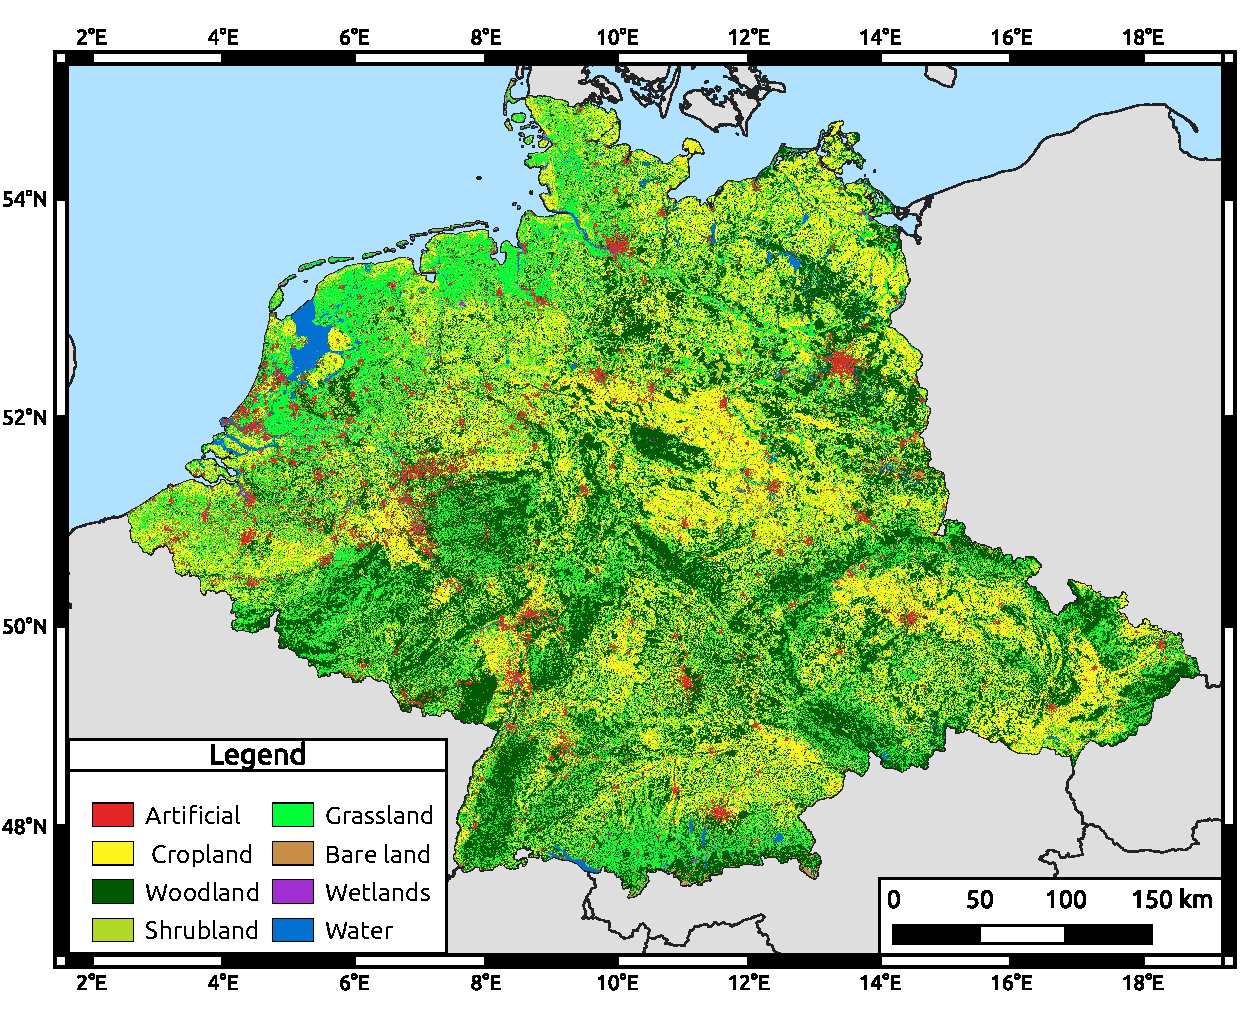
\includegraphics[width=\linewidth]{figs_04/fig4_map.pdf}
        \caption{LUCAS Land cover maps of Belgium, Czechia, Germany, Luxembourg and the Netherlands of 2009 generated with the proposed algorithm, using Eurostat national area estimates and probabilities predicted by the general CatBoost model trained on CORINE centroid points from all countries that implemented LUCAS in 2006.}
        \label{fig:big_map_proportional}
    \end{figure}
    
    \begin{figure}[H]
        \centering
        \includegraphics[width=\linewidth]{figs_04/fig5_example.pdf}
        \caption{Example of the IMP iterative classification process and comparison to highest likelihood classification, using the northwestern outskirts of Apeldoorn, the Netherlands. A: high-resolution reference imagery from Google Earth; B-D: classifications over subsequent iterations, identified in E; F: differences between  the proportional map and the highest likelihood map; G: the highest likelihood map itself.}
        \label{fig:map_example}
    \end{figure}

    A complete overview of the area estimates by Eurostat and mapped area per country, year, class, model type, and map type is included in ~\ref{appendix:full_area_results}. Almost all proportional maps had pixel proportions that fell within the confidence intervals of the Eurostat-derived area estimate. Only some maps derived from probabilities predicted by local models had class proportions that were outside the confidence intervals of the Eurostat area estimates. The only case of underrepresentation was \textit{Bare Land} in the maps derived from probabilities predicted by the local model for Luxembourg, as this class was not represented in the training data. Also in Luxembourg, Woodland was overrepresented by the local model by an average of 0.03 percent above the upper bound of the Eurostat-supplied confidence interval. Both issues are likely due to the fact that Luxembourg's local model was trained on a relatively small dataset compared to the other models, as no under- or overrepresentation occurred in proportional maps derived from probabilities produced by the general model.

    The \textit{Artificial} class was overrepresented in the 2012 map of Germany by 0.04 percent of the upper bound, and finally, the \textit{Shrubland} class was overrepresented in the 2009 map of Czechia by 11 percent. This is the biggest percentual error in all proportional maps, and constitutes a representation of 0.87 percent of Czechia's surface instead of the 0.69 percent estimated by Eurostat, with an upper confidence bound of 0.78 percent. This relatively large overrepresentation was caused after the final iteration, where remaining gaps in the map were filled with the highest likelihood class. These gaps were assigned to \textit{Grassland} and \textit{Shrubland}, for which more pixels were available with higher probabilities. Fig.~\ref{fig:fill_by_iterations} shows how the iterative classification, or 'filling' of the 2009 map of Czechia proceeded. The general behavior of each class is similar to those observed in other countries and years, but not every class approaches the area estimate at the same rate, with \textit{Woodland} reaching the confidence interval at iteration 8, and \textit{Grassland} at iteration 19.
    We observed a similar pattern in other maps: More gaps remained at the final iteration when there was a relatively small surplus of pixels with predicted probabilities for each class. Generally, classes for which there was a low number of pixels with any probability compared to their proportion according to the Eurostat estimate were classified less accurately, and in proportions that less closely matched the Eurostat estimates.
    Predictions by the general model tended to have probabilities for more different classes in each pixel, especially for rarer classes. Fig.~\ref{fig:probability_pixels} shows this for predictions for the Netherlands in 2009. Both models predicted probabilities above zero for \textit{Cropland} and \textit{Grassland} on a large number of pixels compared to their prevalence as estimated by Eurostat, but the local model barely predicted enough pixels for \textit{Bare Land}, and an insufficient amount for \textit{Water}. While the general model predicted a smaller surplus of pixels with probability above zero for Artificial and Woodland, it predicted surpluses for each class. The comparison of Eurostat estimates and counts based on classification in \ref{appendix:full_area_results} show that proportional maps based on probabilities predicted by the general model matched the Eurostat estimates more closely than those based on probabilities predicted by the local model.
    
    \begin{figure}[H]
        \centering
        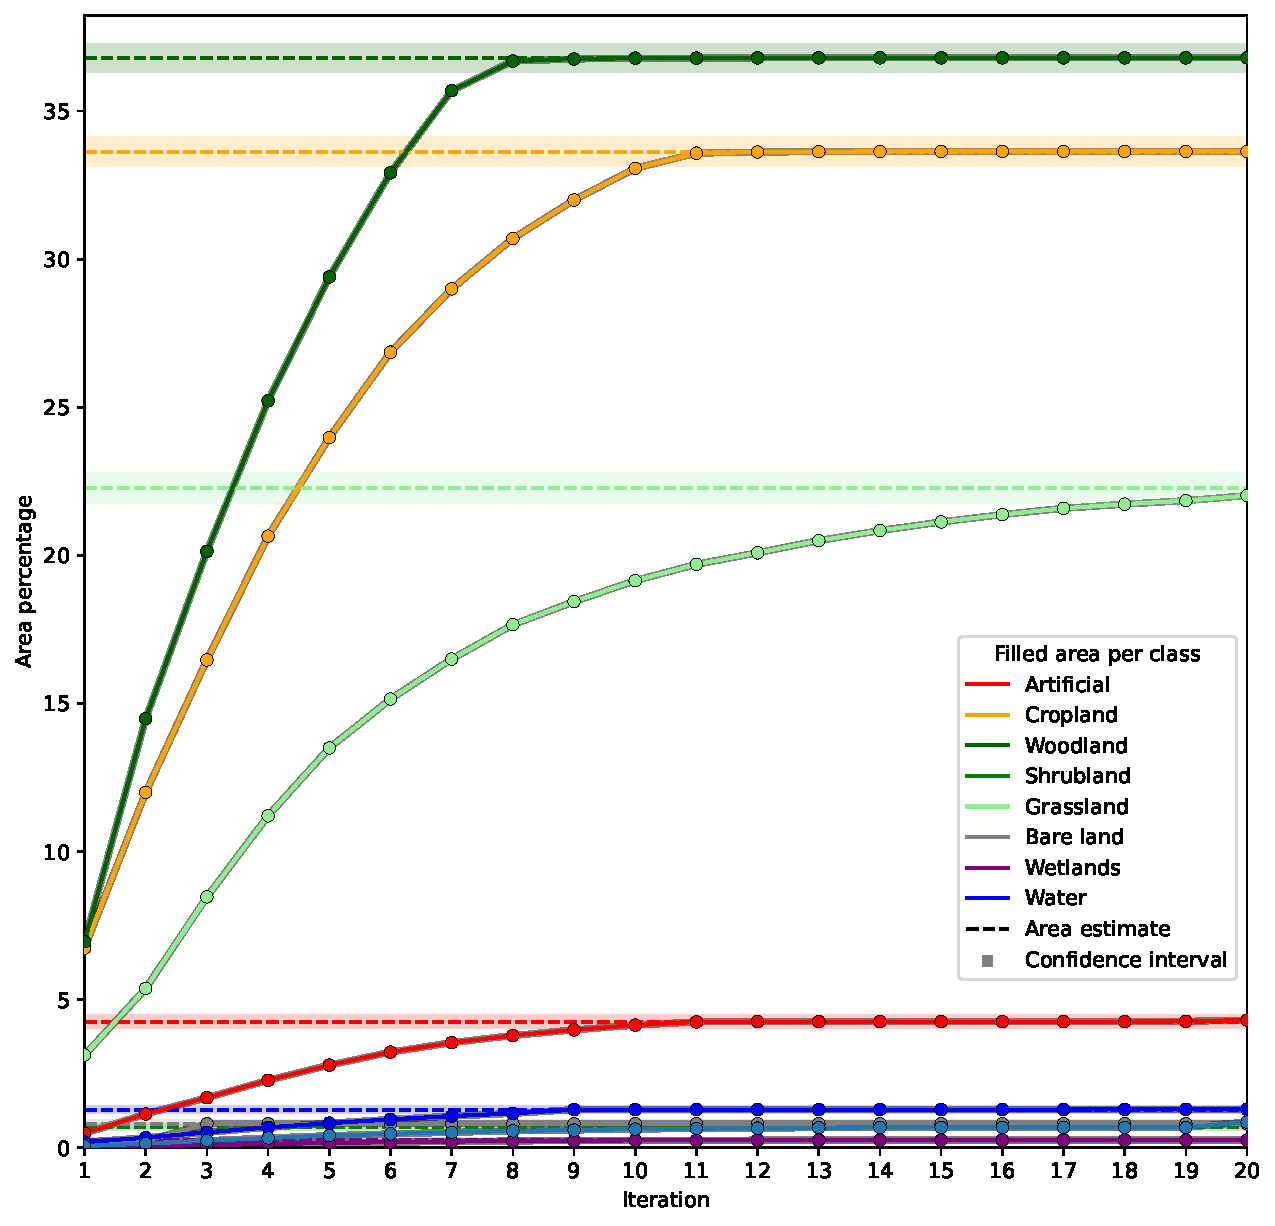
\includegraphics[width=\linewidth]{figs_04/fig6_fill_by_iterations.pdf}
        \caption{Percentage of map area filled per iteration of the IMP algorithm, for the map of Czechia for 2009. Each line with dots indicates the percentage of area assigned to each LUCAS land cover class at each iteration. The dashed lines indicate the mean area estimated by Eurostat, with the lighter-colored area around each dashed line indicating the accompanying confidence interval.}
        \label{fig:fill_by_iterations}
    \end{figure}

    \begin{figure}[H]
        \vspace*{-4cm}
        \centering
        \begin{subfigure}[b]{\textwidth}
            \centering
            \caption{Local Model}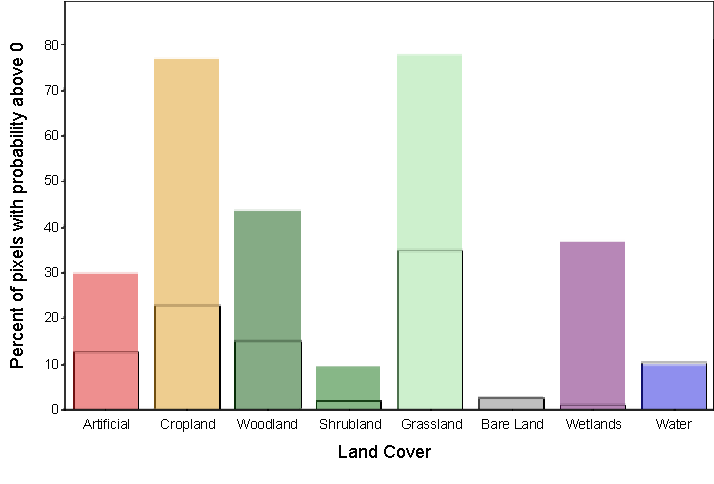
\includegraphics[width=\textwidth]{figs_04/fig7a_probability_pixels_NL_local.pdf}
            \label{fig:probability_pixels_local}
            % \hspace{-0.9em}       
        \end{subfigure}
        \begin{subfigure}[b]{\textwidth}
           \centering
           \caption{General Model}
           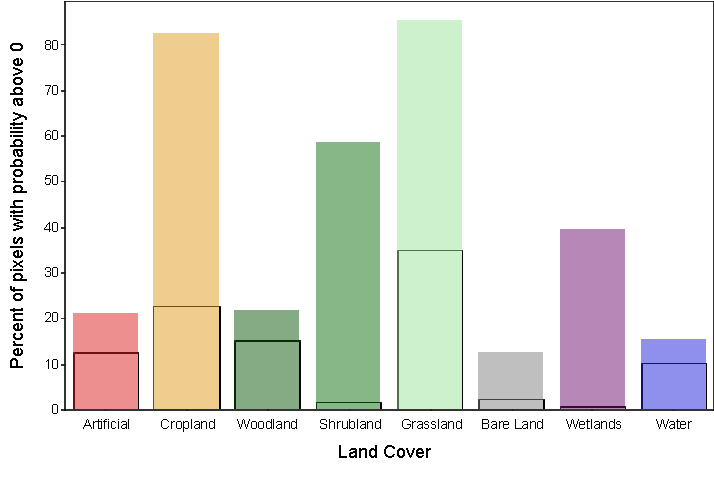
\includegraphics[width=\textwidth]{figs_04/fig7b_probability_pixels_NL_general.pdf}
           \label{fig:probability_pixels_general}   
        \end{subfigure}
        % \vspace*{-0.75cm}
        
        \caption{Percentage of pixels for which any probability above zero was predicted per class, compared to the proportion of that class according to the Eurostat area estimate used to create proportional maps of the Netherlands in 2009. Note that the general model predicted a surplus of probabilities above zero for each class, while the local model did not predict probabilities above zero in enough pixels for \textit{Water}.}
        \label{fig:probability_pixels}
    \end{figure}



    \subsection{Accuracy assessment}
    
    F1-scores calculated by overlaying the highest likelihood and proportional maps of 2009, 2012, 2015 and 2018 on LUCAS points of matching years and the maps of 2017 on S2GLC points show (see Fig.~\ref{fig:f1}) the accuracy of proportional maps tended to be higher or equal to the accuracy of highest likelihood maps. The difference between highest likelihood maps and proportional maps created from the same predicted probabilities is more pronounced on maps created by the general model, which was trained on the entire training dataset. On average across all mapped years (see table \ref{tab:f1_scores}, proportional maps were more accurate than highest likelihood maps in most cases. Proportional maps consistently achieved a weighted F1-score above 0.7 on LUCAS points, and above 0.85 on S2GLC points. Fig.~\ref{fig:precision} shows that the highest likelihood maps generally had higher precision (User's accuracy) than proportional maps, while Fig.~\ref{fig:recall} shows that proportional maps generally had higher recall (Producer's accuracy). This sacrifice of precision for gains in recall can explain the noted increase in F1-score. Note that we use the \textit{weighted} precision and recall metrics to give equal importance to the performance of every class. 
    
    As shown in Fig.~\ref{fig:quantity_disagreement}, the proportional maps had a lower quantity disagreement than the maximum likelihood maps, reducing it to near-zero in most cases. It also shows that maximum likelihood maps based on probabilities predicted by local models tended to be more accurate than those based on probabilities predicted by the general model.

    \begin{table}[H]
    \caption{Comparison of F1-scores for different countries, validation datasets, and model types. The table presents the F1-scores for both highest likelihood and proportional maps across five countries, using two validation datasets (S2GLC and LUCAS) and two model types (local and general). The "Difference" column quantifies the difference in F1-scores between the highest likelihood and proportional maps. Note that the LUCAS values are averages of the 4 years that were mapped and validated: 2009, 2012, 2015 and 2018.}
    \centering
    \label{tab:f1_scores}
    \begin{tabular}{c|c|c|p{2.1cm}|p{2.12cm}|p{2cm}}
    Country & Dataset & Model Type & \multicolumn{3}{c}{F1-score} \\
    \cline{4-6}
           &         &            & Proportional & Highest Likelihood & Difference \\
    \hline
    \multirow{4}{*}{NL} & \multirow{2}{*}{S2GLC} & local & 0.85 & 0.86 & -0.01 \\
                        &                        & general & 0.86 & 0.80 & 0.06 \\
                        & \multirow{2}{*}{LUCAS} & local & 0.71 & 0.72 & -0.01 \\
                        &                        & general & 0.73 & 0.67 & 0.06 \\
    \hline
    \multirow{4}{*}{LU} & \multirow{2}{*}{S2GLC} & local & 0.95 & 0.98 & -0.03 \\
                        &                        & general & 0.97 & 0.91 & 0.06 \\
                        & \multirow{2}{*}{LUCAS} & local & 0.75 & 0.73 & 0.02 \\
                        &                        & general & 0.73 & 0.68 & 0.05 \\
    \hline
    \multirow{4}{*}{DE} & \multirow{2}{*}{S2GLC} & local & 0.94 & 0.93 & 0.01 \\
                        &                        & general & 0.93 & 0.83 & 0.10 \\
                        & \multirow{2}{*}{LUCAS} & local & 0.77 & 0.77 & 0.00 \\
                        &                        & general & 0.76 & 0.70 & 0.06 \\
    \hline
    \multirow{4}{*}{BE} & \multirow{2}{*}{S2GLC} & local & 0.90 & 0.87 & 0.03 \\
                        &                        & general & 0.92 & 0.87 & 0.05 \\
                        & \multirow{2}{*}{LUCAS} & local & 0.71 & 0.71 & 0.00 \\
                        &                        & general & 0.72 & 0.70 & 0.02 \\
    \hline
    \multirow{4}{*}{CZ} & \multirow{2}{*}{S2GLC} & local & 0.94 & 0.91 & 0.03 \\
                        &                        & general & 0.96 & 0.88 & 0.08 \\
                        & \multirow{2}{*}{LUCAS} & local & 0.78 & 0.78 & 0.00 \\
                        &                        & general & 0.78 & 0.73 & 0.05 \\
    \end{tabular}
    \end{table}




    \begin{figure}[H]
        \centering
        \includegraphics[width=\linewidth]{figs_04/fig8_jointplot_F1.pdf}
        \caption{Weighted F1-score of the land cover maps classified with maximum likelihood (X-axis) and the iterative mapping (Y-axis), validated on LUCAS and S2GLC reference data. Maps based on probabilities predicted by the general model are shown in blue, while maps based on probabilities predicted by local models are shown in orange. The boxplots at the top and right summarize the F1-scores of maximum likelihood and proportional classification, respectively. The diagonal reference line shows where the F1-score would be equal, while the horizontal and vertical line represent the average across all F1-scores. Points above the diagonal reference line indicate maps where proportional maps were more accurate. 
        In most cases, proportional maps had higher F1-scores than maximum likelihood maps. This difference was generally larger when using probabilities predicted by the general model, although maps based on predictions by local models were more accurate on average.}
        \label{fig:f1}
    \end{figure}

    \begin{figure}[H]
        \centering
        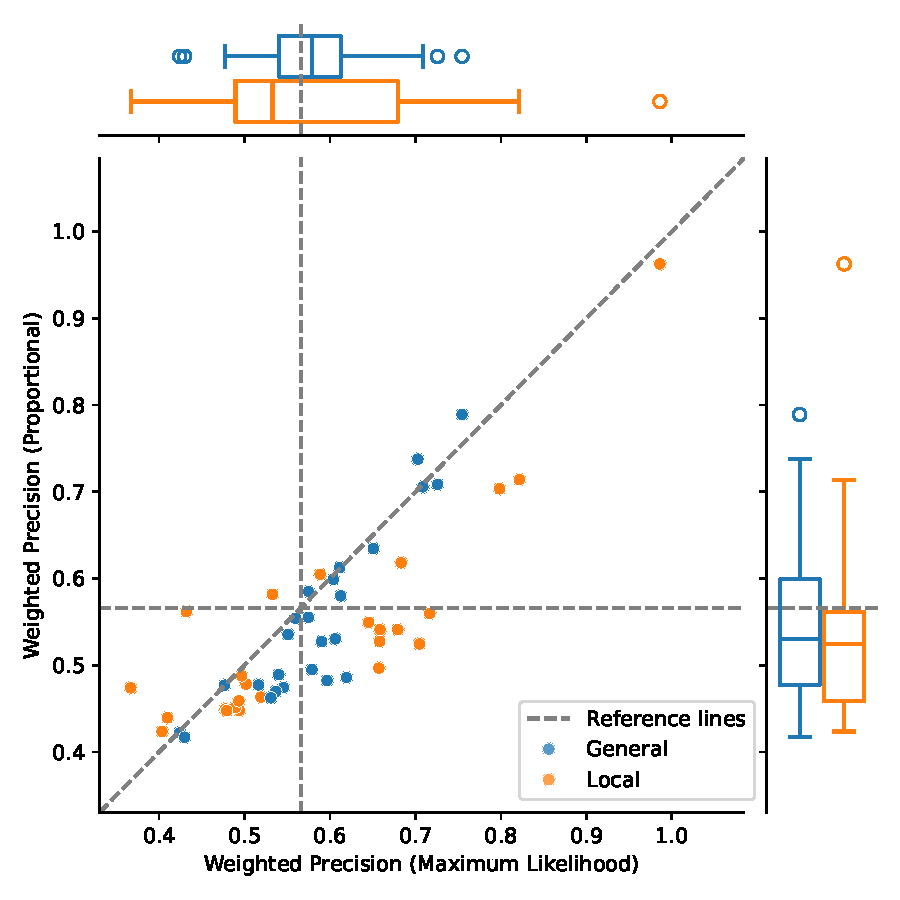
\includegraphics[width=\linewidth]{figs_04/fig9_jointplot_precision.pdf}
        \caption{Weighted precision (User's accuracy) of the land cover maps classified with maximum likelihood (X-axis) and the iterative mapping (Y-axis), validated on LUCAS and S2GLC reference data. Maps based on probabilities predicted by the general model are shown in blue, while maps based on probabilities predicted by local models are shown in orange. The boxplots at the top and right summarize the precision of maximum likelihood and proportional classification, respectively. The diagonal reference line shows where the F1-score would be equal, while the horizontal and vertical line represent the average across all precision scores. Points above the diagonal reference line indicate maps where proportional maps were more precise. 
        Note that proportional maps generally had a lower precision than maximum likelihood maps, and that this difference was bigger for maps based on probabilities predicted by local models.}
        \label{fig:precision}
    \end{figure}

    \begin{figure}[H]
        \centering
        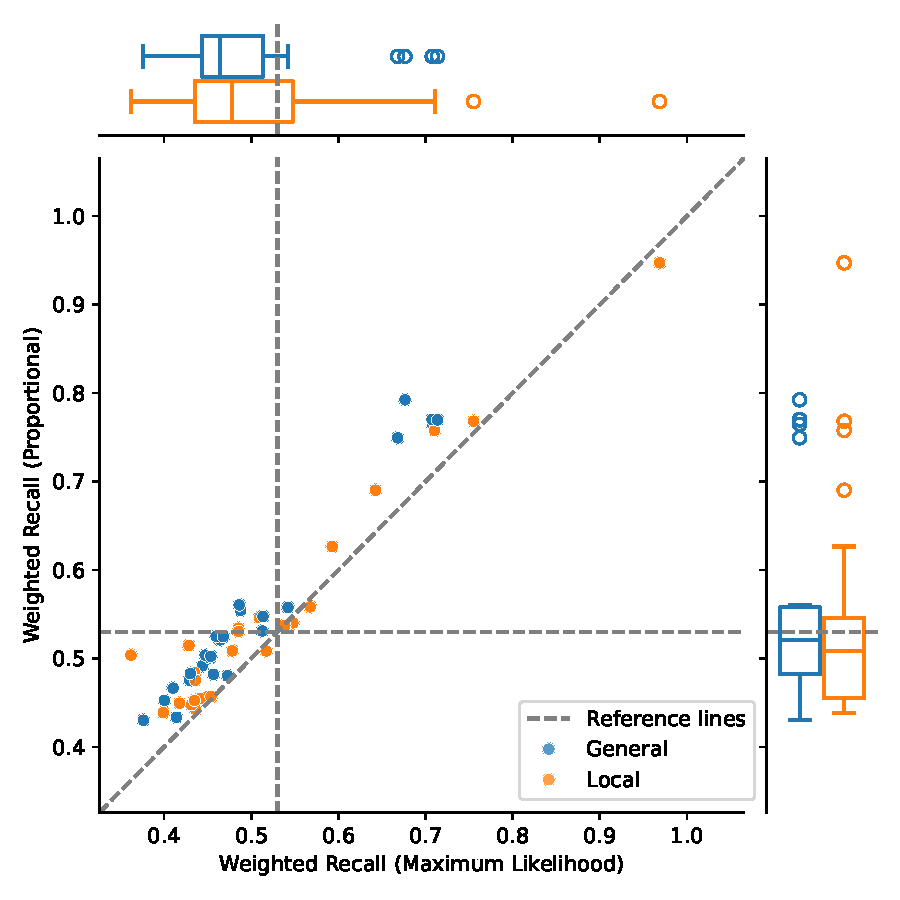
\includegraphics[width=\linewidth]{figs_04/fig10_jointplot_recall.pdf}
        \caption{Weighted recall (Producer's accuracy) of the land cover maps classified with maximum likelihood (X-axis) and the iterative mapping (Y-axis), validated on LUCAS and S2GLC reference data. Maps based on probabilities predicted by the general model are shown in blue, while maps based on probabilities predicted by local models are shown in orange. The boxplots at the top and right summarize the recall of maximum likelihood and proportional classification, respectively. The diagonal reference line shows where the F1-score would be equal, while the horizontal and vertical line represent the average across all recall scores. Points above the diagonal reference line indicate maps where proportional maps had a higher recall. 
        Observations include: 1) Proportional class maps generally exhibit a marginally higher F1-score, 2) The range of quantity error for proportional class maps narrow compared to highest probability class maps, and 3) Highest probability maps generated by the general model were less accurate in terms of both quantity and allocation disagreement than those generated by local models.}
        \label{fig:recall}
    \end{figure}

    \begin{figure}[H]
    \vspace{-2cm}
        \centering
        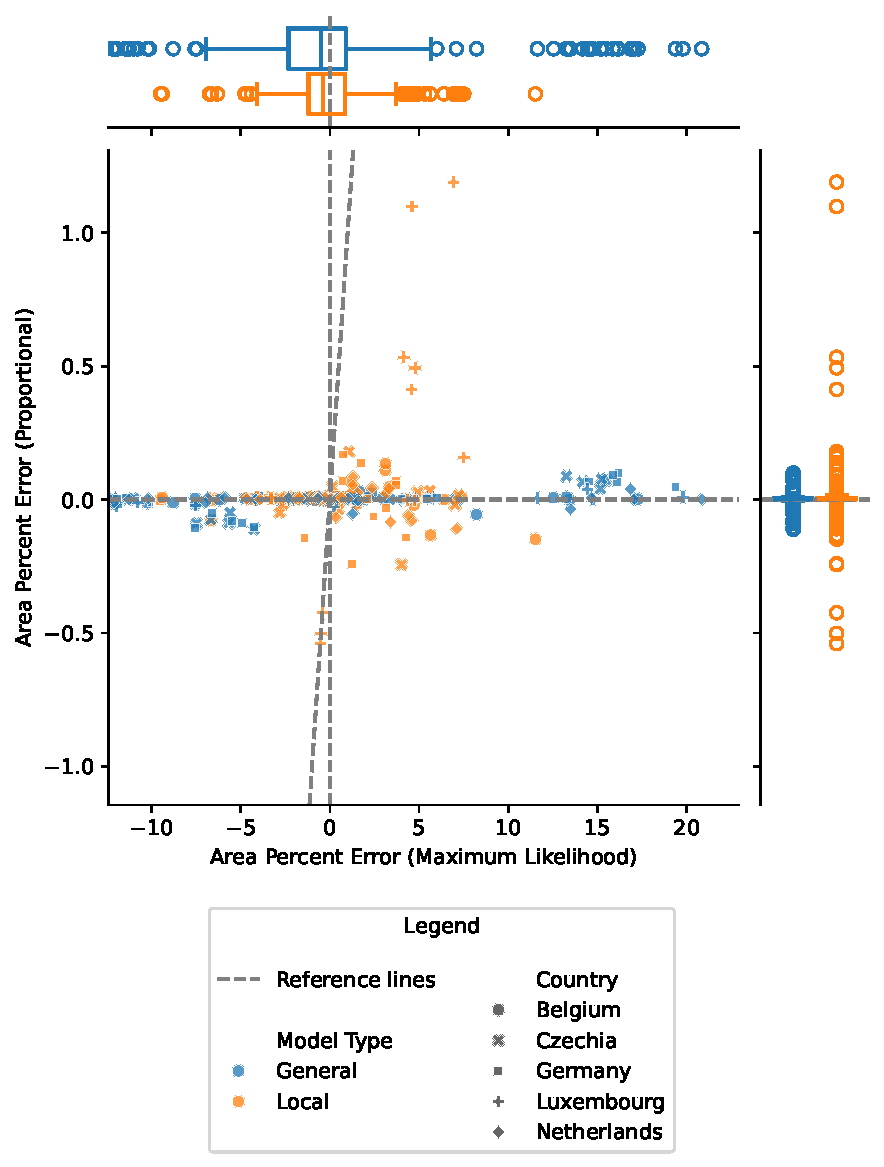
\includegraphics[width=\linewidth]{figs_04/fig11_jointplot_area_percent_error.pdf}
        \caption{Class-wise allocation disagreement of maximum likelihood (X-axis) and proportional (Y-axis) maps based on probabilities predicted by the general model (blue) and local models (orange). Allocation disagreement is quantified as area percent error: the percent point difference between the target area estimate and the amount of pixels classified on the map. Note that proportional maps had errors close to zero, with the exception of Luxembourg (indicated with $+$), and that highest likelihood maps based on probabilities predicted by local models had lower quantity disagreement than those based on predictions by the general model.}
        \label{fig:quantity_disagreement}
    \end{figure}
    
\section{Discussion}

    \subsection{Algorithm design and performance}

        We found that IMP yielded higher accuracy compared to highest probability class assignment. 
    
        Where the use of prior probabilities to adjust classification thresholds such as summarized by \citet{mingguo2009effect} does not guarantee  method proposed by \citep{horvath2021comparison} leaves considerable gaps due to overlapping 'best probability' pixels for several classes, our iterative approach with a decaying threshold minimizes this problem by classifying the best pixels for every class first. Any remaining unclassified pixels can be filled in with the highest likelihood class without severely affecting the distribution of classes. The number of iterations can be increased to improve convergence to area estimates, which might be needed if there are relatively few pixels with probabilities for one or more classes. Using models that push probability mass away from 0 and 1 like boosting \citep{niculescu2005predicting}, as was used in this work, may play a role as well.
    
        We did not expect the proportional maps to be consistently either equally or more accurate than those created by highest likelihood classification. A possible explanation for this improvement in accuracy is that by forcing the classification to be stratified according to an accurate area estimate, we reduce the bias of the model. This is supported by the fact that the difference in accuracy between proportional and highest likelihood class maps was higher when using probabilities predicted by the general model: A general model, having been trained on a dataset that is less representative of any given country, is therefore likely to be more biased \citep{he2009learning}, which gives more space for the iterative algorithm to improve the map. This corresponds to claims by \citet{sales2022land} and \citet{kleinewillinghofer2022unbiased} that area estimates are better derived from predictions by models that were trained on datasets representative of the area of interest.

    \subsection{Limitations and potential improvements}

        While the proposed algorithm correctly mapped to area proportions in most attempts, this is not generally guaranteed. Experiments with different preprocessing workflows, model types, and parameters such as the number of iterations, suggested that the algorithm performs better in both quantity and allocation accuracy when, respectively, more pixels in the area of interest have a predicted probability for multiple classes (see Figs.\ref{fig:fill_by_iterations}~and~\ref{fig:probability_availability_pixels}), and when these probabilities are properly ranked within each class. We did not include these initial experiments for the sake of brevity, but this should be taken into account when applying our method to other probability predictions. Based on our omitted findings about the quantity of pixels with predicted probabilities for any given class, we expect techniques that push probability mass away from extreme values, such as label smoothing \citep{müller2020when} might help the algorithm converge to the area estimates, as more pixels will be available with probabilities for more classes. This might not lead to more accurate maps by itself, however. It is possible that accuracy of proportional maps could be increased by using probabilities that more closely meet the assumption that probabilities are properly ranked, such as those produced by Platt Scaling \citep{niculescu2005predicting}.

    \subsection{Potential applications}

        The primary purpose for which this algorithm was designed is to create, or update, land cover maps based on predicted probabilities, using a given area estimate. This area estimate can be derived from an external source, such as a sample-based measurement, like in the case of this study. However, the algorithm might also be used to update a map used to derive area estimates with post-stratification sampling \citep{olofsson2014good}, using the corrected area estimates and the original probabilities that were used to make the initial map. Besides this purpose, however, we suggest interested parties consider the following:

        Our results show that the single, bigger \textit{general model} was often less accurate when mapping a single area of interest than the \textit{local models} that were trained only on data from their corresponding country. However, this difference in accuracy disappeared in proportional maps, and the general model successfully detected a rare class that was not present in the training data for Luxembourg, whereas the local model simply skipped these classes.

        Additionally, the iterative nature of IMP enables the production of spatially explicit uncertainty assessments. Pixel-level uncertainty is useful because it can be propagated in spatial models that use land cover as a covariate \citep{herold2016toward}. During this study, we found that the pixels classified in earlier iterations have a higher validation allocation disagreement than those classified in later iterations (see Fig.~\ref{fig:f1_score_during_filling} for an example). It is therefore possible to calculate separate precision (User's accuracy) scores per class and per iteration, leading to a more fine-grained indicator of each pixel's reliability for decision makers or use in subsequent modeling. The combination these 'iteration maps' (see Fig.~\ref{fig:map_example}~E)  with the user's accuracy of each iteration needs further study. 

        \begin{figure}
            \vspace*{-4cm}
            \centering
            \begin{subfigure}[b]{0.82\textwidth}
            \centering
            \caption{Local Model}\includegraphics[width=\textwidth]{figs_04/fig12a_f1_during_filling_local.pdf}
            \label{fig:f1_filling_local}
            \hspace{-0.9em}
            
            \end{subfigure}
            
            \begin{subfigure}[b]{0.82\textwidth}
           \centering
           \caption{General Model}
           \includegraphics[width=\textwidth]{figs_04/fig12b_f1_during_filling_general.pdf}
           \label{fig:f1_filling_general}
           
        \end{subfigure}
            \vspace*{-0.75cm}
            \caption{Validation performance of proportional maps compared to the highest likelihood baseline. This example of the weighted F1 score of the partially filled-in map during each iteration of IMP, and a comparison with the weighted F1-score of the highest likelihood map when derived from probabilities predicted by the local (a) and general (b) model. The lines represent validations of all maps of Czechia. Note that the pixels classified at early iterations achieve a higher score, and that the score gradually decreases as a greater number of pixels is classified, stabilizing at or above baseline established by highest likelihood maps.}
            \label{fig:f1_score_during_filling}
        \end{figure}
    
        Furthermore, it is possible that our proposed algorithm might improve the temporal consistency of land cover classification, leading to better land cover change mapping. Due to variations in satellite reflectance per mapped time period, spurious changes are often included in land cover change maps that do not implement proper post-processing techniques. While many such techniques already exist, they often rely on contiguous time series of predictions or are computationally intensive. Our proposed algorithm does not have these limitations, only requiring an up-to-date area estimate of each year, or an interpolation such as the one used to make maps of the year 2017 in this study. If further research indicates that the algorithm can reduce spurious change, it would therefore be a useful addition to the existing methods.
        
        Lastly, during this study it became clear that the method might be suitable for more than only making maps whose proportions match area estimates. The observed improvement in accuracy of proportional maps output by IMP over highest likelihood classification suggests that forcibly improving quantity disagreement with posterior quantity estimates can improve allocation disagreement to a certain extent. This means that IMP could be used to validate area estimates themselves. When provided with 1) a validation dataset that was not used in the area estimation process and suitable for the mapped resolution (such as the S2GLC points in this study), 2) predicted probabilities of sufficient quality, and 3) multiple area estimates, the best area estimate should lead to the most accurate proportional map possible. Exploring this further was beyond the scope of this study but may prove a promising use case.

\section{Conclusion}

    We present an algorithm that can transform predicted probabilities by a given machine learning model into maps whose class proportions match area estimates. Our validation on two independent test datasets (LUCAS and S2GLC points) across five years and five countries show that these maps were also equally, if not more, accurate than maps classified according to the maximum probability per pixel. In our experiments, this increase in accuracy was achieved by sacrificing some degree of precision (User's accuracy) for relatively larger gains in recall (Producer's accuracy). Because pixels classified at each iteration have different precision and recall values, the iteration at which a pixel was classified can be used to approximate pixel-wise uncertainty. 
    IMP greatly improves the accuracy of models trained on a bigger, but imbalanced, training dataset. This means that it can be used to optimize predictions by big models to local contexts if reliable area estimates are available. This offers potential for the increasing number of global and continental-scale maps which are trained on a rich feature space and achieve high overall accuracy, but have also been criticized for their relatively low accuracy and/or usefulness at more local scales. By negating the bias from large scale models, IMP can therefore contribute to make accurate and useful maps of smaller regions. This, combined with the potential to generate pixel-based error estimates, suggests that IMP can be a valuable tool for decision makers and other stakeholders.

\section{Data Availability}
The 400 predicted probability layers, 50 highest likelihood class maps, and 50 proportional class maps, are available on zenodo at https://zenodo.org/records/10641340. This download is accompanied by the used area estimates, and a script that produces proportional maps.

\section{Appendices}

    \subsection*{Training point filtering}
    \label{tab:corine_filtering}
    \begin{table}[H]
    \caption{Point filtering rules per class used to remove potential label errors from the CORINE centroids before using them as training data, as well as the number of points that resulted.}
    
    \begin{tabular}{lrlrr}
    \hline
    LUCAS class    & Condition  & dataset                                      & Source & Removed \\
    \hline
    Artificial     & \verb|>| 150    & OSM Buildings / Cop Imp.  & \citep{witjes2022spatiotemporal}       & 68,444  \\
    Artificial     & \verb|<| 50     & OSM buildings / Cop Imp.  & \citep{witjes2022spatiotemporal}       & 333,526 \\
    Non-Artificial & \verb|> 50 <| 150 & OSM buildings / Cop Imp.  & \citep{witjes2022spatiotemporal}       & 9,594   \\
    Non-Artificial & \verb|>| 30     & Rasterized OSM Roads                       & \citep{witjes2022spatiotemporal}       & 161,576 \\
    Non-Artificial & \verb|>| 30     & Rasterized OSM Railroads                   & \citep{witjes2022spatiotemporal}       & 2,759   \\
    Woodland       & \verb|<| 1      & Cop Tree Cover                      &   \citep{copernicus2023hrl}      & 62,731  \\
    Shrubland      & \verb|>| 50     & Cop Tree Cover                      &  \citep{copernicus2023hrl}       & 121,464 \\
    Shrubland      & \verb|>| 50     & Cop Grassland                       &  \citep{copernicus2023hrl}       & 48,734  \\
    Grassland      & \verb|<| 1      & Cop Grassland                       &  \citep{copernicus2023hrl}       & 174,616 \\
    Grassland      & \verb|>| 30     & Cop Tree Cover                      &  \citep{copernicus2023hrl}       & 48,443  \\
    Bare Land      & \verb|>| 1      & Cop Tree Cover                      &  \citep{copernicus2023hrl}       & 16,156  \\
    Bare Land      & \verb|>| 1      & Cop Grassland                       &  \citep{copernicus2023hrl}       & 11,052  \\
    Wetlands       & \verb|<| 1      & Cop Temp and Perm Wetness &  \citep{copernicus2023hrl}       & 7,973   \\
    Water          & \verb|<| 50     & Cop Permanent Water                 &  \citep{copernicus2023hrl}       & 9,511 \\
    \hline
    \end{tabular}
    \end{table}
    
\subsection*{IMP Algorithm in pseudocode}
    \label{alg:imp}
    \newcommand{\lbox}[2]{\parbox[t]{\dimexpr 0.9\linewidth-#1em}{#2 \strut}}

    \begin{algorithm}[H]
    \caption{Iterative Mapping of Probabilities}
    
    \begin{algorithmic}[1]
    \Statex \textbf{Input:} 
    \Statex \textbullet~$P$, predicted probabilities for each class $C$
    \Statex \textbullet~$E$, the target area estimate 
    \Statex \textbullet~$I$, the number of iterations
    \Statex \textbf{Output:}
    \Statex \textbullet~$M$, the land cover map whose class proportions should match $E$.
    
    \noindent\rule[0.5ex]{\linewidth}{1pt}
    \Statex \textbf{1:} Initialize the empty output map $M$
    \Statex \textbf{2:} \textbf{for} iteration $i = 1$ to $I+1$ \textbf{do}
        \Statex\hspace*{1em} \textbf{2.1} \lbox{1}{Set ratio $r_i$ to $\frac{i}{I}$}
        \Statex\hspace*{1em} \textbf{2.2} \lbox{1}{\textbf{for} each $C$ \textbf{do}}
            \Statex\hspace*{2em} \textbf{2.2.1} \lbox{2}{$E_C$ = The target number of pixels of $C$ in the output $M$ according to $E$}
            \Statex\hspace*{2em} \textbf{2.2.2} \lbox{2}{$M_{Ci}$ = Number of pixels in $M$ already classified as $C$ at $i$}
            \Statex\hspace*{2em} \textbf{2.2.3} \lbox{2}{$N_{Ci}$ = Number of pixels that must still be classified as $C$ to match $E_C$}
            \Statex\hspace*{2em} \textbf{2.2.4} \lbox{2}{$P_C$ = All pixels in $P$ with probability for $C$ above 0}
            \Statex\hspace*{2em} \textbf{2.2.5} \lbox{2}{$P_{Ci}$ = All unclassified pixels in $P_C$}
            \Statex\hspace*{2em} \textbf{2.2.6} \lbox{2}{$E_{Ci}$ = Number of pixels to classify in $i$ = $N_C \times r_i$}
            \Statex\hspace*{2em} \textbf{2.2.7} \lbox{2}{$Q$ = the top $\frac{E_{Ci}}{P_{Ci}}$-th percentile of $P_{Ci}$}
            \Statex\hspace*{2em} \textbf{2.2.8} \lbox{2}{$P_Q$ = The lowest probability among pixels in $Q$}
            \Statex\hspace*{2em} \textbf{2.2.9} \lbox{2}{$N_{CQ}$ = Number of pixels in $P$ with probability values  $\ge{} P_Q$ for $C$.}
            \Statex\hspace*{2em} \textbf{2.2.10} \lbox{2}{\textbf{if} $N_{CQ} > N_{Ci}$ \textbf{do}}
                \Statex\hspace*{3em}\textbullet~\lbox{3}{Select all pixels with probability $\ge{} P_Q + 1$ \& update $N_{CQ}$}
                \Statex\hspace*{3em}\textbullet~\lbox{3}{Randomly sample $N_{CQ}-N_{Ci}$ pixels with probability $P_Q$}
                \Statex\hspace*{3em}\textbullet~\lbox{3}{Classify both pixel groups as $C$}                
            \Statex\hspace*{2em} \textbf{else}
                \Statex\hspace*{3em}\textbullet~\lbox{3}{Classify all pixels in $P_{Ci}$ with probability $\ge{} P_Q$ as $C$.}
    \Statex \textbf{3:} \lbox{0}{Classify all remaining unclassified pixels using highest likelihood classification.}
    \end{algorithmic}
    \end{algorithm}

    \subsection*{Full area results}
    \label{appendix:full_area_results}
    This appendix shows the area per land cover as estimated by Eurostat, predicted by both the country's local model and the general model, and processed into a hard-class map by both highest likelihood classification and iterative mapping of probabilities. The 'Best' columns show which combination of model type and mapping type resulted in a mapped area that most closely matched the mean estimated by Eurostat. The Eurostat 'Min' and 'Max' columns are the estimated mean minus and plus the reported variance of the estimate; these indicate the range that should ideally contain the mapped area. 
    
    
    
    \subsubsection{Belgium}
    Proportional maps of Belgium consistently matched Eurostat area estimates more closely than highest likelihood maps. Out of 5 years for 8 classes, classes mapped from predictions by general models matched Eurostat estimates more closely than those made from predictions by local models 8 times, while classes mapped from local model predictions had a closer match 6 times.
    \begin{table}[H]
    \centering
    \caption{Land cover area estimated by Eurostat and classified by both model (local and general) and map (highest likelihood and proportional) types for BE in 2009.}
    
    \begin{tabular}{r|rrr|rr|rr|rr}
    \toprule
    {} & \multicolumn{3}{|c}{Eurostat} & \multicolumn{2}{|c}{Highest Likelihood} & \multicolumn{2}{|c}{Proportional} & \multicolumn{2}{|c}{Best} \\
    {} &      Min &   Mean &    Max &              Local & General &        Local & General &  Model &    Map \\
    \midrule
    Artificial &     9.39 &   9.92 &  10.45 &              16.32 &   11.58 &         9.92 &    9.95 &  Local &  Prop. \\
    Cropland   &    26.05 &  26.72 &  27.38 &              20.41 &   19.16 &        26.72 &   26.72 &    Tie &  Prop. \\
    Woodland   &    23.88 &  24.54 &   25.2 &               25.0 &   21.31 &        24.54 &   24.54 &    Tie &  Prop. \\
    Shrubland  &     0.79 &   0.94 &   1.09 &               0.96 &    3.27 &         0.94 &    0.96 &  Local &  Prop. \\
    Grassland  &    34.37 &  35.29 &   36.2 &              36.82 &   43.51 &        35.27 &   35.23 &  Local &  Prop. \\
    Bare land  &      0.9 &   1.13 &   1.37 &                0.0 &    0.13 &         1.14 &    1.14 &    Tie &  Prop. \\
    Wetlands   &     0.05 &   0.07 &   0.09 &                0.0 &    0.08 &         0.08 &    0.08 &    Tie &    Tie \\
    Water      &     1.23 &    1.4 &   1.57 &               0.49 &    0.95 &          1.4 &     1.4 &    Tie &  Prop. \\
    \bottomrule
    \end{tabular}
    \end{table}
    
    \begin{table}[H]
    \centering
    \caption{Land cover area estimated by Eurostat and classified by both model (local and general) and map (highest likelihood and proportional) types for BE in 2012.}
    
    \begin{tabular}{r|rrr|rr|rr|rr}
    \toprule
    {} & \multicolumn{3}{|c}{Eurostat} & \multicolumn{2}{|c}{Highest Likelihood} & \multicolumn{2}{|c}{Proportional} & \multicolumn{2}{|c}{Best} \\
    {} &      Min &   Mean &    Max &              Local & General &        Local & General &    Model &    Map \\
    \midrule
    Artificial &    10.33 &  10.84 &  11.35 &              16.15 &   11.48 &        10.85 &   10.85 &      Tie &  Prop. \\
    Cropland   &     28.7 &  29.44 &  30.18 &              19.95 &    16.9 &        29.44 &   29.42 &    Local &  Prop. \\
    Woodland   &    23.75 &  24.31 &  24.87 &              25.23 &    21.2 &        24.31 &   24.31 &      Tie &  Prop. \\
    Shrubland  &     0.74 &   0.85 &   0.97 &               1.39 &    3.83 &         0.86 &    0.86 &      Tie &  Prop. \\
    Grassland  &    31.08 &  31.98 &  32.88 &               36.7 &   45.42 &        31.96 &   31.98 &  General &  Prop. \\
    Bare land  &      0.7 &   0.81 &   0.91 &                0.0 &    0.11 &         0.81 &    0.81 &      Tie &  Prop. \\
    Wetlands   &     0.28 &   0.34 &    0.4 &                0.0 &    0.12 &         0.35 &    0.35 &      Tie &  Prop. \\
    Water      &     1.24 &   1.43 &   1.62 &               0.58 &    0.94 &         1.43 &    1.43 &      Tie &  Prop. \\
    \bottomrule
    \end{tabular}
    \end{table}
    
    \begin{table}[H]
    \centering
    \caption{Land cover area estimated by Eurostat and classified by both model (local and general) and map (highest likelihood and proportional) types for BE in 2015.}
    
    \begin{tabular}{r|rrr|rr|rr|rr}
    \toprule
    {} & \multicolumn{3}{|c}{Eurostat} & \multicolumn{2}{|c}{Highest Likelihood} & \multicolumn{2}{|c}{Proportional} & \multicolumn{2}{|c}{Best} \\
    {} &      Min &   Mean &    Max &              Local & General &        Local & General &    Model &    Map \\
    \midrule
    Artificial &     10.9 &  11.39 &  11.88 &              14.49 &   10.59 &         11.5 &   11.39 &  General &  Prop. \\
    Cropland   &     28.2 &  28.54 &  28.88 &               21.9 &   19.75 &        28.54 &   28.53 &    Local &  Prop. \\
    Woodland   &    24.42 &  24.67 &  24.92 &              25.21 &   21.94 &        24.68 &   24.67 &  General &  Prop. \\
    Shrubland  &     1.56 &   1.63 &    1.7 &               1.14 &    2.94 &         1.63 &    1.63 &      Tie &  Prop. \\
    Grassland  &     30.4 &  31.02 &  31.64 &              36.67 &   43.57 &        30.89 &   31.03 &  General &  Prop. \\
    Bare land  &     0.75 &   0.83 &   0.91 &                0.0 &    0.11 &         0.83 &    0.83 &      Tie &  Prop. \\
    Wetlands   &     0.27 &   0.47 &   0.67 &                0.0 &    0.08 &         0.47 &    0.47 &      Tie &  Prop. \\
    Water      &     1.29 &   1.45 &   1.61 &               0.59 &    1.01 &         1.46 &    1.46 &      Tie &  Prop. \\
    \bottomrule
    \end{tabular}
    \end{table}
    
    \begin{table}[H]
    \centering
    \caption{Land cover area estimated by Eurostat and classified by both model (local and general) and map (highest likelihood and proportional) types for BE in 2017.}
    
    \begin{tabular}{r|rrr|rr|rr|rr}
    \toprule
    {} & \multicolumn{3}{|c}{Eurostat} & \multicolumn{2}{|c}{Highest Likelihood} & \multicolumn{2}{|c}{Proportional} & \multicolumn{2}{|c}{Best} \\
    {} &      Min &   Mean &    Max &              Local & General &        Local & General &    Model &    Map \\
    \midrule
    Artificial &    11.13 &  11.62 &  12.12 &              14.75 &   10.74 &        11.76 &   11.63 &  General &  Prop. \\
    Cropland   &    28.53 &  28.89 &  29.26 &              19.49 &   18.67 &         28.9 &   28.88 &    Local &  Prop. \\
    Woodland   &     25.6 &  25.86 &  26.12 &              23.47 &   19.67 &        25.86 &   25.86 &      Tie &  Prop. \\
    Shrubland  &     1.33 &   1.39 &   1.45 &               1.13 &    3.24 &         1.39 &    1.39 &      Tie &  Prop. \\
    Grassland  &    28.51 &  29.11 &  29.71 &              40.63 &   46.39 &        28.96 &   29.11 &  General &  Prop. \\
    Bare land  &     1.33 &   1.44 &   1.55 &                0.0 &    0.11 &         1.45 &    1.45 &      Tie &  Prop. \\
    Wetlands   &     0.31 &   0.46 &    0.6 &                0.0 &    0.16 &         0.46 &    0.46 &      Tie &  Prop. \\
    Water      &      1.1 &   1.22 &   1.34 &               0.54 &    1.02 &         1.23 &    1.23 &      Tie &  Prop. \\
    \bottomrule
    \end{tabular}
    \end{table}
    
    \begin{table}[H]
    \centering
    \caption{Land cover area estimated by Eurostat and classified by both model (local and general) and map (highest likelihood and proportional) types for BE in 2018.}
    
    \begin{tabular}{r|rrr|rr|rr|rr}
    \toprule
    {} & \multicolumn{3}{|c}{Eurostat} & \multicolumn{2}{|c}{Highest Likelihood} & \multicolumn{2}{|c}{Proportional} & \multicolumn{2}{|c}{Best} \\
    {} &      Min &   Mean &    Max &              Local & General &        Local & General &    Model &    Map \\
    \midrule
    Artificial &    11.25 &  11.74 &  12.24 &              15.07 &   10.72 &        11.79 &   11.75 &  General &  Prop. \\
    Cropland   &    28.69 &  29.07 &  29.44 &               22.4 &   21.55 &        28.99 &   29.05 &  General &  Prop. \\
    Woodland   &    26.19 &  26.46 &  26.72 &              25.02 &   21.66 &        26.46 &   26.46 &      Tie &  Prop. \\
    Shrubland  &     1.21 &   1.27 &   1.33 &               1.39 &    3.41 &         1.28 &    1.28 &      Tie &  Prop. \\
    Grassland  &    27.56 &  28.15 &  28.74 &              35.54 &   41.43 &        28.16 &   28.16 &      Tie &  Prop. \\
    Bare land  &     1.63 &   1.75 &   1.87 &                0.0 &    0.12 &         1.76 &    1.76 &      Tie &  Prop. \\
    Wetlands   &     0.33 &   0.45 &   0.57 &                0.0 &    0.09 &         0.46 &    0.46 &      Tie &  Prop. \\
    Water      &     1.01 &   1.11 &   1.21 &               0.58 &    1.01 &         1.11 &    1.11 &      Tie &  Prop. \\
    \bottomrule
    \end{tabular}
    \end{table}
    
    \subsubsection{Czechia}
    Proportional maps of Czechia consistently matched Eurostat area estimates more closely than highest likelihood maps. Out of 5 years for 8 classes, classes mapped from predictions by general models matched Eurostat estimates more closely than those made from predictions by local models 4 times, while classes mapped from local model predictions had a closer match 9 times.
    
    \begin{table}[H]
    \centering
    \caption{Land cover area estimated by Eurostat and classified by both model (local and general) and map (highest likelihood and proportional) types for CZ in 2009.}
    
    \begin{tabular}{r|rrr|rr|rr|rr}
    \toprule
    {} & \multicolumn{3}{|c}{Eurostat} & \multicolumn{2}{|c}{Highest Likelihood} & \multicolumn{2}{|c}{Proportional} & \multicolumn{2}{|c}{Best} \\
    {} &      Min &   Mean &    Max &              Local & General &        Local & General &    Model &    Map \\
    \midrule
    Artificial &     4.05 &   4.26 &   4.47 &               4.41 &     4.0 &         4.31 &    4.27 &  General &  Prop. \\
    Cropland   &    33.16 &  33.63 &  34.11 &               31.7 &   26.96 &        33.64 &   33.56 &    Local &  Prop. \\
    Woodland   &    36.35 &   36.8 &  37.24 &              34.74 &   23.82 &         36.8 &    36.8 &      Tie &  Prop. \\
    Shrubland  &      0.6 &   0.69 &   0.78 &               1.77 &    7.78 &         0.87 &    0.69 &  General &  Prop. \\
    Grassland  &    21.77 &  22.26 &  22.75 &              26.28 &   36.44 &        22.02 &   22.33 &  General &  Prop. \\
    Bare land  &      0.7 &   0.81 &   0.92 &                0.0 &    0.05 &         0.81 &    0.81 &      Tie &  Prop. \\
    Wetlands   &     0.19 &   0.26 &   0.32 &               0.28 &    0.06 &         0.26 &    0.26 &      Tie &  Prop. \\
    Water      &     1.19 &   1.29 &   1.39 &               0.83 &    0.89 &          1.3 &     1.3 &      Tie &  Prop. \\
    \bottomrule
    \end{tabular}
    \end{table}
    
    \begin{table}[H]
    \centering
    \caption{Land cover area estimated by Eurostat and classified by both model (local and general) and map (highest likelihood and proportional) types for CZ in 2012.}
    
    \begin{tabular}{r|rrr|rr|rr|rr}
    \toprule
    {} & \multicolumn{3}{|c}{Eurostat} & \multicolumn{2}{|c}{Highest Likelihood} & \multicolumn{2}{|c}{Proportional} & \multicolumn{2}{|c}{Best} \\
    {} &      Min &   Mean &    Max &              Local & General &        Local & General &  Model &    Map \\
    \midrule
    Artificial &     4.21 &   4.41 &   4.61 &               4.42 &    4.13 &         4.41 &    4.41 &    Tie &  Prop. \\
    Cropland   &    32.21 &  32.84 &  33.46 &              30.03 &   25.35 &        32.79 &   32.75 &  Local &  Prop. \\
    Woodland   &     37.0 &  37.72 &  38.43 &              35.21 &   25.57 &        37.72 &   37.72 &    Tie &  Prop. \\
    Shrubland  &     0.67 &   0.78 &   0.89 &               1.63 &    6.43 &         0.79 &    0.79 &    Tie &  Prop. \\
    Grassland  &    20.95 &  21.99 &  23.02 &               27.6 &   37.47 &        22.02 &   22.06 &  Local &  Prop. \\
    Bare land  &      0.6 &    0.7 &   0.79 &                0.0 &    0.06 &          0.7 &     0.7 &    Tie &  Prop. \\
    Wetlands   &     0.14 &   0.18 &   0.21 &               0.25 &    0.06 &         0.18 &    0.18 &    Tie &  Prop. \\
    Water      &     1.14 &   1.39 &   1.65 &               0.86 &    0.95 &          1.4 &     1.4 &    Tie &  Prop. \\
    \bottomrule
    \end{tabular}
    \end{table}
    
    \begin{table}[H]
    \centering
    \caption{Land cover area estimated by Eurostat and classified by both model (local and general) and map (highest likelihood and proportional) types for CZ in 2015.}
    
    \begin{tabular}{r|rrr|rr|rr|rr}
    \toprule
    {} & \multicolumn{3}{|c}{Eurostat} & \multicolumn{2}{|c}{Highest Likelihood} & \multicolumn{2}{|c}{Proportional} & \multicolumn{2}{|c}{Best} \\
    {} &      Min &   Mean &    Max &              Local & General &        Local & General &    Model &    Map \\
    \midrule
    Artificial &     4.42 &   4.62 &   4.83 &               3.82 &    3.71 &         4.63 &    4.63 &      Tie &  Prop. \\
    Cropland   &    31.77 &  32.03 &  32.29 &              31.72 &   27.78 &        32.04 &   31.92 &    Local &  Prop. \\
    Woodland   &    37.27 &  37.53 &  37.79 &              34.64 &   26.23 &        37.53 &   37.53 &      Tie &  Prop. \\
    Shrubland  &     0.93 &    1.0 &   1.07 &               1.49 &    5.63 &         0.96 &     1.0 &  General &  Prop. \\
    Grassland  &    22.07 &  22.31 &  22.56 &              27.25 &   35.57 &        22.34 &    22.4 &    Local &  Prop. \\
    Bare land  &     0.81 &   0.87 &   0.92 &                0.0 &    0.06 &         0.87 &    0.87 &      Tie &  Prop. \\
    Wetlands   &     0.23 &   0.26 &   0.29 &               0.21 &    0.07 &         0.26 &    0.26 &      Tie &  Prop. \\
    Water      &     1.33 &   1.38 &   1.43 &               0.86 &    0.95 &         1.38 &    1.38 &      Tie &  Prop. \\
    \bottomrule
    \end{tabular}
    \end{table}
    
    \begin{table}[H]
    \centering
    \caption{Land cover area estimated by Eurostat and classified by both model (local and general) and map (highest likelihood and proportional) types for CZ in 2017.}
    
    \begin{tabular}{r|rrr|rr|rr|rr}
    \toprule
    {} & \multicolumn{3}{|c}{Eurostat} & \multicolumn{2}{|c}{Highest Likelihood} & \multicolumn{2}{|c}{Proportional} & \multicolumn{2}{|c}{Best} \\
    {} &      Min &   Mean &    Max &              Local & General &        Local & General &  Model &    Map \\
    \midrule
    Artificial &     4.32 &   4.46 &   4.59 &               4.22 &    3.91 &         4.46 &    4.46 &    Tie &  Prop. \\
    Cropland   &    32.93 &  33.17 &  33.41 &               30.9 &   27.57 &        33.17 &   33.12 &  Local &  Prop. \\
    Woodland   &    37.82 &  38.06 &  38.31 &              34.82 &   27.07 &        38.07 &   38.07 &    Tie &  Prop. \\
    Shrubland  &     0.94 &    1.0 &   1.06 &               1.11 &    4.36 &          1.0 &     1.0 &    Tie &  Prop. \\
    Grassland  &    20.64 &  20.86 &  21.08 &              27.87 &   36.04 &        20.84 &    20.9 &  Local &  Prop. \\
    Bare land  &     0.82 &   0.87 &   0.93 &                0.0 &    0.04 &         0.88 &    0.88 &    Tie &  Prop. \\
    Wetlands   &     0.27 &   0.29 &   0.32 &               0.19 &    0.06 &          0.3 &     0.3 &    Tie &  Prop. \\
    Water      &     1.24 &   1.29 &   1.33 &               0.89 &    0.96 &         1.29 &    1.29 &    Tie &  Prop. \\
    \bottomrule
    \end{tabular}
    \end{table}
    
    \begin{table}[H]
    \centering
    \caption{Land cover area estimated by Eurostat and classified by both model (local and general) and map (highest likelihood and proportional) types for CZ in 2018.}
    
    \begin{tabular}{r|rrr|rr|rr|rr}
    \toprule
    {} & \multicolumn{3}{|c}{Eurostat} & \multicolumn{2}{|c}{Highest Likelihood} & \multicolumn{2}{|c}{Proportional} & \multicolumn{2}{|c}{Best} \\
    {} &      Min &   Mean &    Max &              Local & General &        Local & General &  Model &    Map \\
    \midrule
    Artificial &     4.28 &   4.37 &   4.47 &               4.41 &    4.16 &         4.38 &    4.38 &    Tie &  Prop. \\
    Cropland   &     33.5 &  33.74 &  33.97 &              31.13 &   28.08 &        33.72 &   33.65 &  Local &  Prop. \\
    Woodland   &     38.1 &  38.33 &  38.56 &              34.67 &   26.14 &        38.34 &   38.34 &    Tie &  Prop. \\
    Shrubland  &     0.95 &    1.0 &   1.06 &               1.41 &    5.21 &          1.0 &     1.0 &    Tie &  Prop. \\
    Grassland  &    19.93 &  20.13 &  20.33 &              27.34 &   35.37 &        20.15 &   20.21 &  Local &  Prop. \\
    Bare land  &     0.82 &   0.88 &   0.93 &                0.0 &    0.05 &         0.88 &    0.88 &    Tie &  Prop. \\
    Wetlands   &     0.28 &   0.31 &   0.33 &               0.17 &    0.05 &         0.31 &    0.31 &    Tie &  Prop. \\
    Water      &      1.2 &   1.24 &   1.28 &               0.86 &    0.93 &         1.24 &    1.24 &    Tie &  Prop. \\
    \bottomrule
    \end{tabular}
    \end{table}
    
    
    \subsubsection{Germany}
    Proportional maps of Germany consistently matched Eurostat area estimates more closely than highest likelihood maps, with the exception of a tie for Artificial land cover in 2017. Out of 5 years for 8 classes, classes mapped from predictions by general models matched Eurostat estimates more closely than those made from predictions by local models 7 times, while classes mapped from local model predictions had a closer match 6 times.
    \begin{table}[H]
    \centering
    \caption{Land cover area estimated by Eurostat and classified by both model (local and general) and map (highest likelihood and proportional) types for DE in 2009.}
    
    \begin{tabular}{r|rrr|rr|rr|rr}
    \toprule
    {} & \multicolumn{3}{|c}{Eurostat} & \multicolumn{2}{|c}{Highest Likelihood} & \multicolumn{2}{|c}{Proportional} & \multicolumn{2}{|c}{Best} \\
    {} &      Min &   Mean &    Max &              Local & General &        Local & General &    Model &    Map \\
    \midrule
    Artificial &      6.7 &   6.84 &   6.98 &                7.6 &    5.69 &         6.91 &    6.84 &  General &  Prop. \\
    Cropland   &    32.04 &  32.27 &   32.5 &              35.96 &   26.77 &        32.34 &   32.19 &    Local &  Prop. \\
    Woodland   &    32.09 &  32.28 &  32.47 &               30.7 &   20.18 &        32.28 &   32.28 &      Tie &  Prop. \\
    Shrubland  &     0.86 &   0.91 &   0.97 &               0.94 &    6.29 &         0.92 &    0.92 &      Tie &  Prop. \\
    Grassland  &    24.49 &  24.74 &  24.99 &              23.32 &   39.26 &         24.6 &   24.81 &  General &  Prop. \\
    Bare land  &     0.76 &   0.81 &   0.85 &               0.11 &    0.33 &         0.81 &    0.81 &      Tie &  Prop. \\
    Wetlands   &     0.36 &   0.38 &   0.41 &               0.15 &    0.25 &         0.39 &    0.39 &      Tie &  Prop. \\
    Water      &      1.7 &   1.76 &   1.83 &                1.2 &    1.23 &         1.77 &    1.77 &      Tie &  Prop. \\
    \bottomrule
    \end{tabular}
    \end{table}
    
    \begin{table}[H]
    \centering
    \caption{Land cover area estimated by Eurostat and classified by both model (local and general) and map (highest likelihood and proportional) types for DE in 2012.}
    
    \begin{tabular}{r|rrr|rr|rr|rr}
    \toprule
    {} & \multicolumn{3}{|c}{Eurostat} & \multicolumn{2}{|c}{Highest Likelihood} & \multicolumn{2}{|c}{Proportional} & \multicolumn{2}{|c}{Best} \\
    {} &      Min &   Mean &    Max &              Local & General &        Local & General &    Model &    Map \\
    \midrule
    Artificial &     6.93 &   7.06 &   7.19 &                7.8 &    5.78 &         7.23 &    7.06 &  General &  Prop. \\
    Cropland   &    31.88 &  32.21 &  32.53 &              33.38 &   24.65 &        32.27 &    32.1 &    Local &  Prop. \\
    Woodland   &    32.51 &   32.8 &   33.1 &              31.43 &   21.35 &        32.81 &   32.81 &      Tie &  Prop. \\
    Shrubland  &     1.01 &   1.12 &   1.22 &               0.98 &    6.54 &         1.12 &    1.12 &      Tie &  Prop. \\
    Grassland  &    23.27 &  23.62 &  23.97 &              24.88 &    39.8 &        23.38 &   23.72 &  General &  Prop. \\
    Bare land  &     0.83 &   0.89 &   0.94 &               0.11 &    0.34 &         0.89 &    0.89 &      Tie &  Prop. \\
    Wetlands   &     0.48 &   0.53 &   0.58 &               0.16 &    0.27 &         0.53 &    0.53 &      Tie &  Prop. \\
    Water      &     1.65 &   1.78 &    1.9 &               1.25 &    1.27 &         1.78 &    1.78 &      Tie &  Prop. \\
    \bottomrule
    \end{tabular}
    \end{table}
    
    \begin{table}[H]
    \centering
    \caption{Land cover area estimated by Eurostat and classified by both model (local and general) and map (highest likelihood and proportional) types for DE in 2015.}
    
    \begin{tabular}{r|rrr|rr|rr|rr}
    \toprule
    {} & \multicolumn{3}{|c}{Eurostat} & \multicolumn{2}{|c}{Highest Likelihood} & \multicolumn{2}{|c}{Proportional} & \multicolumn{2}{|c}{Best} \\
    {} &      Min &   Mean &    Max &              Local & General &        Local & General &    Model &    Map \\
    \midrule
    Artificial &      7.2 &   7.38 &   7.57 &               7.73 &    5.75 &          7.4 &    7.38 &  General &  Prop. \\
    Cropland   &    31.72 &  32.27 &  32.82 &              34.37 &   27.34 &        32.27 &   32.18 &    Local &  Prop. \\
    Woodland   &    32.54 &  33.79 &  35.04 &              30.41 &   21.87 &        33.79 &   33.79 &      Tie &  Prop. \\
    Shrubland  &     0.92 &   1.06 &    1.2 &               0.92 &    5.22 &         1.06 &    1.06 &      Tie &  Prop. \\
    Grassland  &    21.14 &  21.88 &  22.63 &              25.04 &   37.99 &        21.85 &   21.95 &    Local &  Prop. \\
    Bare land  &     1.03 &   1.23 &   1.43 &               0.09 &    0.29 &         1.24 &    1.24 &      Tie &  Prop. \\
    Wetlands   &     0.46 &   0.57 &   0.69 &               0.17 &    0.23 &         0.58 &    0.58 &      Tie &  Prop. \\
    Water      &     1.55 &   1.82 &   2.08 &               1.27 &    1.31 &         1.82 &    1.82 &      Tie &  Prop. \\
    \bottomrule
    \end{tabular}
    \end{table}
    
    \begin{table}[H]
    \centering
    \caption{Land cover area estimated by Eurostat and classified by both model (local and general) and map (highest likelihood and proportional) types for DE in 2017.}
    
    \begin{tabular}{r|rrr|rr|rr|rr}
    \toprule
    {} & \multicolumn{3}{|c}{Eurostat} & \multicolumn{2}{|c}{Highest Likelihood} & \multicolumn{2}{|c}{Proportional} & \multicolumn{2}{|c}{Best} \\
    {} &      Min &   Mean &    Max &              Local & General &        Local & General &    Model &    Map \\
    \midrule
    Artificial &     7.11 &    7.5 &   7.88 &                7.5 &    5.65 &          7.5 &     7.5 &      Tie &    Tie \\
    Cropland   &    31.77 &  32.27 &  32.78 &              34.03 &   25.65 &        32.41 &   32.22 &  General &  Prop. \\
    Woodland   &    33.21 &  34.34 &  35.47 &              30.61 &   21.22 &        34.34 &   34.34 &      Tie &  Prop. \\
    Shrubland  &     0.94 &   1.07 &   1.19 &               0.87 &    5.09 &         1.07 &    1.07 &      Tie &  Prop. \\
    Grassland  &    20.47 &  21.13 &  21.79 &              25.42 &   40.51 &        20.99 &   21.18 &  General &  Prop. \\
    Bare land  &     1.18 &   1.38 &   1.57 &               0.11 &    0.32 &         1.38 &    1.38 &      Tie &  Prop. \\
    Wetlands   &     0.48 &   0.57 &   0.66 &               0.18 &    0.28 &         0.57 &    0.57 &      Tie &  Prop. \\
    Water      &     1.53 &   1.75 &   1.97 &               1.27 &    1.29 &         1.75 &    1.75 &      Tie &  Prop. \\
    \bottomrule
    \end{tabular}
    \end{table}
    
    \begin{table}[H]
    \centering
    \caption{Land cover area estimated by Eurostat and classified by both model (local and general) and map (highest likelihood and proportional) types for DE in 2018.}
    
    \begin{tabular}{r|rrr|rr|rr|rr}
    \toprule
    {} & \multicolumn{3}{|c}{Eurostat} & \multicolumn{2}{|c}{Highest Likelihood} & \multicolumn{2}{|c}{Proportional} & \multicolumn{2}{|c}{Best} \\
    {} &      Min &   Mean &    Max &              Local & General &        Local & General &  Model &    Map \\
    \midrule
    Artificial &     7.07 &   7.56 &   8.04 &                7.5 &    5.61 &         7.56 &    7.56 &    Tie &  Prop. \\
    Cropland   &    31.79 &  32.27 &  32.76 &              34.72 &   28.01 &        32.21 &   32.17 &  Local &  Prop. \\
    Woodland   &    33.54 &  34.61 &  35.69 &              30.95 &   20.83 &        34.62 &   34.62 &    Tie &  Prop. \\
    Shrubland  &     0.95 &   1.07 &   1.19 &               0.83 &    7.07 &         1.08 &    1.08 &    Tie &  Prop. \\
    Grassland  &    20.13 &  20.76 &  21.38 &              24.47 &   36.63 &        20.81 &   20.85 &  Local &  Prop. \\
    Bare land  &     1.25 &   1.45 &   1.64 &                0.1 &    0.33 &         1.45 &    1.45 &    Tie &  Prop. \\
    Wetlands   &     0.49 &   0.56 &   0.64 &               0.16 &    0.22 &         0.57 &    0.57 &    Tie &  Prop. \\
    Water      &     1.51 &   1.72 &   1.92 &               1.26 &     1.3 &         1.72 &    1.72 &    Tie &  Prop. \\
    \bottomrule
    \end{tabular}
    \end{table}
    
    \subsubsection{Luxembourg}
    Proportional maps of the Netherlands consistently matched Eurostat area estimates more closely than highest likelihood maps, with the exception of ties for the Wetlands class, which was estimated at zero percent by Eurostat and not predicted inside Luxembourg by any of the general models. Out of 5 years for 8 classes, classes mapped from predictions by general model matched Eurostat estimates more closely than those made from predictions by local models 12 times, while classes mapped from local model predictions had a closer match 6 times.
    
    \begin{table}[H]
    \centering
    \caption{Land cover area estimated by Eurostat and classified by both model (local and general) and map (highest likelihood and proportional) types for LU in 2009.}
    
    \begin{tabular}{r|rrr|rr|rr|rr}
    \toprule
    {} & \multicolumn{3}{|c}{Eurostat} & \multicolumn{2}{|c}{Highest Likelihood} & \multicolumn{2}{|c}{Proportional} & \multicolumn{2}{|c}{Best} \\
    {} &      Min &   Mean &    Max &              Local & General &        Local & General &    Model &    Map \\
    \midrule
    Artificial &     7.59 &   8.86 &  10.13 &               5.56 &    5.65 &         8.86 &    8.86 &      Tie &  Prop. \\
    Cropland   &    16.53 &  18.45 &  20.37 &              25.96 &   10.93 &        18.61 &   18.43 &  General &  Prop. \\
    Woodland   &    31.34 &  33.55 &  35.77 &              38.16 &   32.97 &        34.65 &   33.56 &  General &  Prop. \\
    Shrubland  &     0.44 &   0.69 &   0.94 &               0.01 &    1.58 &          0.7 &     0.7 &      Tie &  Prop. \\
    Grassland  &    33.51 &  36.86 &  40.22 &              30.11 &    48.5 &        36.87 &   36.87 &      Tie &  Prop. \\
    Bare land  &    -0.08 &   1.27 &   2.63 &                0.0 &    0.02 &          0.0 &    1.28 &  General &  Prop. \\
    Wetlands   &      0.0 &    0.0 &    0.0 &                0.2 &     0.0 &          0.0 &     0.0 &      Tie &    Tie \\
    Water      &     -0.0 &   0.31 &   0.62 &                0.0 &    0.34 &         0.31 &    0.31 &      Tie &  Prop. \\
    \bottomrule
    \end{tabular}
    \end{table}
    
    \begin{table}[H]
    \centering
    \caption{Land cover area estimated by Eurostat and classified by both model (local and general) and map (highest likelihood and proportional) types for LU in 2012.}
    
    \begin{tabular}{r|rrr|rr|rr|rr}
    \toprule
    {} & \multicolumn{3}{|c}{Eurostat} & \multicolumn{2}{|c}{Highest Likelihood} & \multicolumn{2}{|c}{Proportional} & \multicolumn{2}{|c}{Best} \\
    {} &      Min &   Mean &    Max &              Local & General &        Local & General &    Model &    Map \\
    \midrule
    Artificial &     8.29 &   9.71 &  11.12 &               5.62 &    5.53 &         9.71 &    9.71 &      Tie &  Prop. \\
    Cropland   &    19.05 &   20.8 &  22.55 &              25.17 &   10.03 &         20.8 &   20.79 &    Local &  Prop. \\
    Woodland   &    31.09 &  32.55 &  34.01 &              39.48 &   34.24 &        33.74 &   32.55 &  General &  Prop. \\
    Shrubland  &     0.62 &   1.23 &   1.84 &               0.01 &    1.18 &         1.24 &    1.23 &  General &  Prop. \\
    Grassland  &    31.53 &   33.9 &  36.27 &               29.5 &   48.65 &         33.9 &    33.9 &      Tie &  Prop. \\
    Bare land  &     0.28 &   1.19 &    2.1 &                0.0 &    0.02 &          0.0 &     1.2 &  General &  Prop. \\
    Wetlands   &      0.0 &    0.0 &    0.0 &               0.23 &     0.0 &          0.0 &     0.0 &      Tie &    Tie \\
    Water      &     0.34 &   0.62 &   0.89 &                0.0 &    0.34 &         0.62 &    0.62 &      Tie &  Prop. \\
    \bottomrule
    \end{tabular}
    \end{table}
    
    \begin{table}[H]
    \centering
    \caption{Land cover area estimated by Eurostat and classified by both model (local and general) and map (highest likelihood and proportional) types for LU in 2015.}
    
    \begin{tabular}{r|rrr|rr|rr|rr}
    \toprule
    {} & \multicolumn{3}{|c}{Eurostat} & \multicolumn{2}{|c}{Highest Likelihood} & \multicolumn{2}{|c}{Proportional} & \multicolumn{2}{|c}{Best} \\
    {} &      Min &   Mean &    Max &              Local & General &        Local & General &    Model &    Map \\
    \midrule
    Artificial &     8.74 &   9.82 &   10.9 &               5.74 &     6.0 &         9.83 &    9.83 &      Tie &  Prop. \\
    Cropland   &     22.4 &  23.31 &  24.21 &              24.89 &   11.38 &        23.31 &   23.29 &    Local &  Prop. \\
    Woodland   &    33.53 &  33.94 &  34.34 &              38.52 &   31.49 &        34.35 &   33.94 &  General &  Prop. \\
    Shrubland  &     3.05 &   3.31 &   3.57 &               0.01 &    2.09 &         3.32 &    3.32 &      Tie &  Prop. \\
    Grassland  &    28.26 &  28.89 &  29.53 &              30.62 &   48.69 &        28.89 &    28.9 &    Local &  Prop. \\
    Bare land  &     0.36 &   0.42 &   0.49 &                0.0 &    0.01 &          0.0 &    0.43 &  General &  Prop. \\
    Wetlands   &      0.0 &    0.0 &    0.0 &               0.22 &     0.0 &          0.0 &     0.0 &      Tie &    Tie \\
    Water      &     0.29 &   0.31 &   0.33 &                0.0 &    0.33 &         0.31 &    0.31 &      Tie &  Prop. \\
    \bottomrule
    \end{tabular}
    \end{table}
    
    \begin{table}[H]
    \centering
    \caption{Land cover area estimated by Eurostat and classified by both model (local and general) and map (highest likelihood and proportional) types for LU in 2017.}
    
    \begin{tabular}{r|rrr|rr|rr|rr}
    \toprule
    {} & \multicolumn{3}{|c}{Eurostat} & \multicolumn{2}{|c}{Highest Likelihood} & \multicolumn{2}{|c}{Proportional} & \multicolumn{2}{|c}{Best} \\
    {} &      Min &   Mean &    Max &              Local & General &        Local & General &    Model &    Map \\
    \midrule
    Artificial &     7.37 &   8.23 &    9.1 &               6.07 &     5.9 &         8.24 &    8.24 &      Tie &  Prop. \\
    Cropland   &    21.47 &  22.28 &  23.09 &              23.93 &   10.32 &        22.29 &   22.26 &    Local &  Prop. \\
    Woodland   &    34.17 &  34.54 &   34.9 &              39.32 &   32.79 &        35.03 &   34.54 &  General &  Prop. \\
    Shrubland  &     2.18 &   2.41 &   2.64 &               0.01 &    2.05 &         2.42 &    2.42 &      Tie &  Prop. \\
    Grassland  &    30.83 &  31.54 &  32.26 &              30.46 &   48.57 &        31.55 &   31.55 &      Tie &  Prop. \\
    Bare land  &     0.43 &    0.5 &   0.57 &                0.0 &    0.01 &          0.0 &    0.51 &  General &  Prop. \\
    Wetlands   &      0.0 &    0.0 &    0.0 &                0.2 &     0.0 &          0.0 &     0.0 &      Tie &    Tie \\
    Water      &     0.46 &   0.49 &   0.52 &                0.0 &    0.35 &         0.49 &    0.49 &      Tie &  Prop. \\
    \bottomrule
    \end{tabular}
    \end{table}
    
    \begin{table}[H]
    \centering
    \caption{Land cover area estimated by Eurostat and classified by both model (local and general) and map (highest likelihood and proportional) types for LU in 2018.}
    
    \begin{tabular}{r|rrr|rr|rr|rr}
    \toprule
    {} & \multicolumn{3}{|c}{Eurostat} & \multicolumn{2}{|c}{Highest Likelihood} & \multicolumn{2}{|c}{Proportional} & \multicolumn{2}{|c}{Best} \\
    {} &      Min &   Mean &    Max &              Local & General &        Local & General &    Model &    Map \\
    \midrule
    Artificial &     6.68 &   7.44 &    8.2 &               5.59 &    5.42 &         7.44 &    7.44 &      Tie &  Prop. \\
    Cropland   &    21.01 &  21.77 &  22.53 &               26.5 &   11.65 &        21.77 &   21.77 &      Tie &  Prop. \\
    Woodland   &    34.49 &  34.84 &  35.18 &              38.98 &   33.08 &        35.37 &   34.84 &  General &  Prop. \\
    Shrubland  &     1.75 &   1.97 &   2.18 &                0.0 &     2.2 &         1.97 &    1.94 &    Local &  Prop. \\
    Grassland  &    32.11 &  32.87 &  33.63 &              28.78 &   47.31 &        32.88 &   32.91 &    Local &  Prop. \\
    Bare land  &     0.46 &   0.54 &   0.62 &                0.0 &    0.01 &          0.0 &    0.54 &  General &  Prop. \\
    Wetlands   &      0.0 &    0.0 &    0.0 &               0.14 &     0.0 &          0.0 &     0.0 &      Tie &    Tie \\
    Water      &     0.54 &   0.58 &   0.62 &                0.0 &    0.34 &         0.58 &    0.58 &      Tie &  Prop. \\
    \bottomrule
    \end{tabular}
    \end{table}
    
    
    \subsubsection{Netherlands}
    Proportional maps of the Netherlands consistently matched Eurostat area estimates more closely than highest likelihood maps. Out of 5 years for 8 classes, classes mapped from predictions by general models matched Eurostat estimates more closely than those made from predictions by local models 15 times, while classes mapped from local model predictions had a closer match 4 times.
    
    \begin{table}[H]
    \centering
    \caption{Land cover area estimated by Eurostat and classified by both model (local and general) and map (highest likelihood and proportional) types for NL in 2009.}
    
    \begin{tabular}{r|rrr|rr|rr|rr}
    \toprule
    {} & \multicolumn{3}{|c}{Eurostat} & \multicolumn{2}{|c}{Highest Likelihood} & \multicolumn{2}{|c}{Proportional} & \multicolumn{2}{|c}{Best} \\
    {} &      Min &   Mean &    Max &              Local & General &        Local & General &    Model &    Map \\
    \midrule
    Artificial &    10.39 &  10.83 &  11.27 &              12.47 &   10.93 &        10.83 &   10.83 &      Tie &  Prop. \\
    Cropland   &    23.04 &  23.73 &  24.41 &              21.38 &   13.52 &        23.73 &   23.73 &      Tie &  Prop. \\
    Woodland   &    11.37 &  11.85 &  12.32 &               15.0 &    7.68 &        11.87 &   11.85 &  General &  Prop. \\
    Shrubland  &     1.75 &    2.0 &   2.26 &               0.82 &    3.57 &         2.01 &    2.01 &      Tie &  Prop. \\
    Grassland  &     38.8 &  39.72 &  40.63 &              40.05 &   53.21 &        39.65 &   39.68 &  General &  Prop. \\
    Bare land  &      1.0 &   1.25 &   1.51 &               0.32 &    0.72 &         1.26 &    1.26 &      Tie &  Prop. \\
    Wetlands   &     0.19 &   0.24 &    0.3 &               1.81 &    1.25 &         0.27 &    0.25 &  General &  Prop. \\
    Water      &     9.92 &  10.38 &  10.84 &               8.16 &    9.12 &        10.39 &   10.38 &  General &  Prop. \\
    \bottomrule
    \end{tabular}
    \end{table}
    
    \begin{table}[H]
    \centering
    \caption{Land cover area estimated by Eurostat and classified by both model (local and general) and map (highest likelihood and proportional) types for NL in 2012.}
    
    \begin{tabular}{r|rrr|rr|rr|rr}
    \toprule
    {} & \multicolumn{3}{|c}{Eurostat} & \multicolumn{2}{|c}{Highest Likelihood} & \multicolumn{2}{|c}{Proportional} & \multicolumn{2}{|c}{Best} \\
    {} &      Min &   Mean &    Max &              Local & General &        Local & General &    Model &    Map \\
    \midrule
    Artificial &    11.04 &  11.48 &  11.92 &               12.0 &   10.88 &        11.48 &   11.48 &      Tie &  Prop. \\
    Cropland   &    23.56 &  24.19 &  24.82 &              19.43 &    12.1 &         24.2 &   24.18 &    Local &  Prop. \\
    Woodland   &     11.7 &  12.13 &  12.55 &              15.44 &    7.97 &        12.17 &   12.13 &  General &  Prop. \\
    Shrubland  &     1.76 &   1.96 &   2.17 &                0.9 &    3.44 &         1.97 &    1.97 &      Tie &  Prop. \\
    Grassland  &    36.35 &  37.24 &  38.13 &              41.84 &   54.31 &        37.16 &   37.24 &  General &  Prop. \\
    Bare land  &     1.34 &    1.5 &   1.65 &               0.34 &     0.8 &          1.5 &     1.5 &      Tie &  Prop. \\
    Wetlands   &     0.48 &   0.58 &   0.67 &               1.73 &    1.37 &          0.6 &    0.58 &  General &  Prop. \\
    Water      &    10.02 &  10.92 &  11.83 &               8.32 &    9.12 &        10.93 &   10.93 &      Tie &  Prop. \\
    \bottomrule
    \end{tabular}
    \end{table}
    
    \begin{table}[H]
    \centering
    \caption{Land cover area estimated by Eurostat and classified by both model (local and general) and map (highest likelihood and proportional) types for NL in 2015.}
    
    \begin{tabular}{r|rrr|rr|rr|rr}
    \toprule
    {} & \multicolumn{3}{|c}{Eurostat} & \multicolumn{2}{|c}{Highest Likelihood} & \multicolumn{2}{|c}{Proportional} & \multicolumn{2}{|c}{Best} \\
    {} &      Min &   Mean &    Max &              Local & General &        Local & General &    Model &    Map \\
    \midrule
    Artificial &    11.67 &  12.14 &   12.6 &              12.19 &   10.65 &        12.14 &   12.14 &      Tie &  Prop. \\
    Cropland   &    23.98 &  24.17 &  24.36 &              20.25 &   12.91 &        24.17 &   24.17 &      Tie &  Prop. \\
    Woodland   &    12.91 &  13.02 &  13.12 &              15.37 &    8.39 &        13.06 &   13.02 &  General &  Prop. \\
    Shrubland  &     1.88 &   2.02 &   2.17 &               0.91 &    3.31 &         2.03 &    1.97 &    Local &  Prop. \\
    Grassland  &    35.89 &  36.29 &  36.69 &               40.7 &   53.15 &        36.23 &   36.33 &  General &  Prop. \\
    Bare land  &     0.86 &   0.94 &   1.01 &               0.34 &    0.72 &         0.94 &    0.94 &      Tie &  Prop. \\
    Wetlands   &     0.92 &   1.05 &   1.19 &               1.75 &    1.46 &         1.06 &    1.06 &      Tie &  Prop. \\
    Water      &     9.96 &  10.37 &  10.79 &                8.5 &     9.4 &        10.38 &   10.38 &      Tie &  Prop. \\
    \bottomrule
    \end{tabular}
    \end{table}
    
    \begin{table}[H]
    \centering
    \caption{Land cover area estimated by Eurostat and classified by both model (local and general) and map (highest likelihood and proportional) types for NL in 2017.}
    
    \begin{tabular}{r|rrr|rr|rr|rr}
    \toprule
    {} & \multicolumn{3}{|c}{Eurostat} & \multicolumn{2}{|c}{Highest Likelihood} & \multicolumn{2}{|c}{Proportional} & \multicolumn{2}{|c}{Best} \\
    {} &      Min &   Mean &    Max &              Local & General &        Local & General &    Model &    Map \\
    \midrule
    Artificial &    12.01 &  12.45 &  12.89 &              12.06 &   10.41 &        12.45 &   12.45 &      Tie &  Prop. \\
    Cropland   &    23.03 &  23.22 &   23.4 &              18.55 &   10.64 &        23.22 &    23.2 &    Local &  Prop. \\
    Woodland   &    14.29 &  14.39 &   14.5 &              15.29 &    7.53 &         14.4 &    14.4 &      Tie &  Prop. \\
    Shrubland  &     1.69 &   1.81 &   1.93 &                0.8 &    3.17 &         1.82 &    1.81 &  General &  Prop. \\
    Grassland  &    34.95 &  35.34 &  35.73 &              42.44 &   56.19 &        35.23 &   35.34 &  General &  Prop. \\
    Bare land  &     1.67 &    1.8 &   1.92 &               0.32 &    0.77 &          1.8 &     1.8 &      Tie &  Prop. \\
    Wetlands   &     0.75 &   0.83 &   0.92 &               2.14 &    1.92 &         0.92 &    0.84 &  General &  Prop. \\
    Water      &     9.77 &  10.16 &  10.55 &               8.39 &    9.36 &        10.17 &   10.17 &      Tie &  Prop. \\
    \bottomrule
    \end{tabular}
    \end{table}
    
    \begin{table}[H]
    \centering
    \caption{Land cover area estimated by Eurostat and classified by both model (local and general) and map (highest likelihood and proportional) types for NL in 2018.}
    
    \begin{tabular}{r|rrr|rr|rr|rr}
    \toprule
    {} & \multicolumn{3}{|c}{Eurostat} & \multicolumn{2}{|c}{Highest Likelihood} & \multicolumn{2}{|c}{Proportional} & \multicolumn{2}{|c}{Best} \\
    {} &      Min &   Mean &    Max &              Local & General &        Local & General &    Model &    Map \\
    \midrule
    Artificial &    12.18 &   12.6 &  13.03 &              11.88 &   10.29 &        12.61 &   12.61 &      Tie &  Prop. \\
    Cropland   &    22.56 &  22.74 &  22.92 &              22.47 &   15.78 &        22.75 &   22.73 &    Local &  Prop. \\
    Woodland   &    14.98 &  15.08 &  15.19 &              15.71 &    9.18 &        15.09 &   15.09 &      Tie &  Prop. \\
    Shrubland  &      1.6 &    1.7 &   1.81 &               0.97 &     3.3 &         1.71 &     1.7 &  General &  Prop. \\
    Grassland  &    34.48 &  34.86 &  35.25 &              38.26 &   49.53 &        34.78 &   34.87 &  General &  Prop. \\
    Bare land  &     2.07 &   2.23 &   2.38 &               0.34 &    0.78 &         2.23 &    2.23 &      Tie &  Prop. \\
    Wetlands   &     0.66 &   0.73 &   0.79 &               2.01 &    1.75 &         0.78 &    0.73 &  General &  Prop. \\
    Water      &     9.68 &  10.05 &  10.43 &               8.35 &     9.4 &        10.06 &   10.06 &      Tie &  Prop. \\
    \bottomrule
    \end{tabular}
    \end{table}
	\chapter[Synthesis]{Synthesis}
\label{cha:Chapter6}
\newpage

This thesis aims to contribute towards efforts made in large-scale land cover mapping, with an emphasis on the benefits of combining several datasets from different sources and of different types. It presents different steps of a methodology to extract training data from multiple rich human-annotated datasets and overlay them on Earth observation data from diverse sources. It furthermore details the challenges and benefits of creating land cover maps that navigate the trade-off between spatial, temporal, and thematic resolution, as well as quantity and allocation accuracy.

This thesis, especially in its first two chapters, describes a relatively applied line of research. Besides the chapters themselves, several datasets were produced, and have been published as open data (CC-BY license):
\begin{enumerate}
    \item 2000-2020 quarterly Landsat composites at 30~m resolution and 7 bands (on \url{stac.ecodatacube.eu});
    \item 2016-2019 quarterly/annual Sentinel-2 composites at 10--30m resolution, depending on the band (on \url{stac.ecodatacube.eu});
    \item Harmonized LUCAS and CORINE training points for LULC classification \citep{landa2021multi};
    \item Input dataset for gap filling and land cover mapping using the eumap library \citep{parente2020input};
    \item An Ensemble Digital Terrain Model of Europe at 30~m resolution \citep{hengl2021continental}
    \item 2000-2019 annual Land Use / Land Cover maps of Europe at 30m resolution and 43 classes \citep{parente2021continental};
    \item Five annual land cover maps of five European countries (Belgium, Czechia, Germany, Luxembourg and The Netherlands) at 30m resolution and 8 classes, whose class proportions match Eurostat area estimates \citep{witjes2024iterative_data}.
\end{enumerate}
The third chapter of the thesis describes relatively more innovative attempts to model land cover in a way that is faithful to area estimates. The proposed algorithm (IMP) may have further uses and implications, these will also be discussed in this synthesis chapter. It is divided into two sections: the first summarizes contributions to the research objectives formulated in Section~\ref{sec:research_objectives} and the second section reflects on these contributions, offering perspectives on future research opportunities. 

\section{Main Findings}
    The chapters of this thesis all address multiple research questions. Their results will be discussed from the perspective of the research questions; each question is discussed below.
    
    \subsection{What are the benefits and challenges of combining multiple large time-series and static EO datasets into Analysis-Ready Data for the purpose of land cover classification?}
    \label{syn:rq1}

        This research question was largely explored in Chapters\@~\ref{cha:chapter2}\@~and\@~\ref{cha:chapter3}. Chapter\@~\ref{cha:chapter2} details the construction of an Earth observation data cube from various sources (Landsat, Sentinel-2 and several DTMs), and includes experiments that investigate the performance of land cover models using different combinations of these datasets. Chapter\@~\ref{cha:chapter3} uses most of this data cube to train a single LULC classification model, which is subsequently used to create annual maps of Europe between 2000 and 2019. 

        \subsubsection{Benefits}
    
            Our land cover experiments in Chapter\@~\ref{cha:chapter2} show that random forest models trained on the largest combination of datasets achieved a higher classification accuracy than models trained only on data from one satellite program during both cross-validation (0.761 vs 0.741) and on the test set (0.774 vs 0.768). This is in line with other work reporting that including auxiliary variables in the feature space can improve performance \citep{zhu2016optimizing, hurskainen2019auxiliary, hosseiny2022urban, santos2012multiscale}.

            Chapter\@~\ref{cha:chapter2} also details the creation of an Ensemble DTM which was more accurate than its four source datasets, with a RMSE 6.544 vs RMSE of 8.451-9.900. This demonstrates that in the case of continuous variables, different versions or representations of that variable can be used as input for a machine learning algorithm, and that the predictions by this algorithm can be more accurate.
            
            In Chapter\@~\ref{cha:chapter3}, the top 15 most important variables of the ensemble land cover model contain data from six sources: several bands from two satellite programs (Landsat and MODIS), long-term probability of surface water occurrence \citep{pekel2016high}, geometric temperature \citep{kilibarda2014spatio}, multiple DTM variables, and the cost distance to the nearest coastline (see Fig.~\ref{fig:variable_importance}). 
    
        \subsubsection{Challenges}
            
            Experiments in Chapter\@~\ref{cha:chapter2} showed that models using the full feature space (Landsat, Sentinel-2 and DTM) achieved the highest classification accuracy, with different datasets improving the results for different land cover classes. This is supported by variable importance in Chapter \ref{cha:chapter3}: data from four different sources (Landsat, surface water frequency, DTM, and distance to coast) were among the top 15 of 200 variables for LULC modeling. While it is clear that combining different datasets into one feature space can improve model performance, there are some challenges:
    
            \textbf{Spatial resolution}: Overlaying different raster datasets onto training samples may yield high accuracy (like in Chapter\@~\ref{cha:chapter2}), but can cause artifacts in the shape of low-resolution raster cells when creating maps at the highest resolution among the used datasets. Fortunately, recent findings suggest that certain modeling techniques, such as convolutional neural networks, can counteract this effect \citep{robinson2019large}. In Chapters\@~\ref{cha:chapter3}\@~and\@~\ref{cha:chapter4}, we used low-resolution MODIS data as part of the feature space. To avoid artifacts, we smoothed it while resampling it to a 30~m resolution, but this is a very unsophisticated method and may have led to the loss of a lot of explanatory power. This is also reflected by its low position in the variable importance of the ensemble model in Chapter\@~\ref{cha:chapter3}.

            \textbf{Temporal resolution} can be subdivided into the temporal resolution of the feature space and that of the mapped units. It is essential to have a high temporal resolution in the feature space to correctly detect and distinguish different vegetation types due to the temporal dynamics of their phenology. The time range represented by a single map has different implications for the accuracy of different classes. In Chapters\@~\ref{cha:chapter3}\@~and\@~\ref{cha:chapter4}, we chose to make annual maps, and in Chapter\@~\ref{cha:chapter3}, we made annual maps for each consecutive year. This does not work equally well for each class. For example, mapping classes that only periodically cover a certain patch of ground, such as crops, or areas that are prone to different water levels, such as flood plains. At a high thematic resolution, this problem may be minimal: a change of crops due to crop rotation will still be cropland, but when mapping different crops, this will quickly become problematic. Another example from Chapter\@~\ref{cha:chapter3} is \textit{Burnt areas}, which was among the least accurately mapped classes. This is likely due to the fact that these areas don't stay \textit{Burnt} for a long time.

        In conclusion, integrating large time-series and static Earth observation datasets into Analysis-Ready Data can enhance land cover classification accuracy. However, challenges such as spatial resolution discrepancies, temporal resolution constraints, and class balance issues present hurdles that must be addressed to make full use of their potential.
            
    \subsection{To what extent does training data from multiple times and places improve the accuracy and generalization of land cover classification?}
    \label{syn:rq2}
    
        The land cover experiments in Chapters 2 and 3 investigate the generalization potential of models trained on data from a single year, and those trained on data from several years. Results from both chapters show that models trained on samples from different years were more accurate; both on years with available training data, and on unseen years. 
        
        In the land cover classification experiments of Chapter~\ref{cha:chapter2}, the model that was trained on a small multi-year Landsat-only data outperformed the model trained on Landsat, sentinel, and DTM data on the test set. This suggests that there is a unique benefit in training a model on data from a larger time range.
        
        In Chapter~\ref{cha:chapter3}, we combined LUCAS points with samples extracted from CORINE polygons to create a training dataset with samples from 8 years (see table~\ref{tab:cv_annual}). On average, models trained on CORINE and LUCAS points from multiple years were more accurate (0.543 vs 0.498) than those trained only on one year when validated on points from 2018, which was left out of the training set in that experiment. We did notice that training on the LUCAS data lead to lower accuracy than on only CORINE (0.579) across all experiments, whether it be in combination with CORINE points (0.543) or stand-alone (0.491). This is likely because the LUCAS points are a stricter validation set, whose class only describes a 10~m square. Leveraging the higher amount of points available from using a multi-year dataset improved generalization accuracy on 2018 by 1\% and accuracy on trained years by 2\%. Cross-validation of the final model showed that the weighted F1-score of the model was more consistent through time than through space (with standard deviations of 0.135 per year and 0.150 per 30~km tile, respectively). While this is only a small increase, we achieved high accuracy when validating our map of 2017 on the points collected by \citep{jenerowicz2021validation} to validate the S2GLC maps made by \citet{malinowski2020automated}: We achieved a similar accuracy without having training data from 2017 and operating on a lower spatial resolution.

        \subsubsection{Dealing with bias}
        
        Combining training data from multiple sources and a wide range of locations and times can introduce bias in the model because the proportion of classes might not match the proportions on the ground in the mapped area in a given time frame. Collecting land cover observations from multiple sources requires consideration of the quality and type of each component dataset. which all have their own problems. For instance, we tried to reproduce the CORINE land cover legend at 30~m resolution, but some classes, such as \textit{urban fabric}, don't directly translate to \textit{buildings} at CORINE's large minimal mapping unit. This can lead to sampled points of an urban area falling within a garden, and therefore being a bad example of a 'buildings' class. Furthermore, some classes with small or narrow patches (e.g., roads) can be relatively rare at the scale of CORINE, which leads to under-representation in the resulting 30~m training set. 

        In Chapter\@~\ref{cha:chapter3}, we did not pay any attention to this issue and selected one point per polygon, which led to some classes being drastically underrepresented and more inaccurately classified than expected, even with a large legend of heterogeneous combinations of land use and land cover classes such as CORINE. In chapters 2 and 4, we only used the LUCAS points because the emphasis was on the benefits of combining EO data sources and the effects of the IMP algorithm, respectively. In future research, a logical improvement to the point sample extraction from polygons will be to sample several points from each polygon, and having the number be dependent on the size and land cover class of the polygon. The scarcity of narrow and small-polygon classes is best dealt with by integrating more different datasets, such as OpenStreetMap for roads, and EUBUCCO for buildings \citep{milojevic2023eubucco}. In volunteered geographical information, errors can come from different sources. For example, when collecting \textit{Buildings} data from OpenStreetMap for Chapter\@~\ref{cha:chapter3}, we encountered buildings labeled in many different terms, including \textit{residential}, personal names, \textit{yes}, and, perplexingly, \textit{no}. To correctly capture the right instances of a class, these issues need to be dealt with.
        
        Our results in Chapter\@~\ref{cha:chapter3} show that the ensemble model was much less accurate in Southern Europe than in Central and Northern Europe. We found a weak but significant positive correlation between the number of training samples and the F1-score in 30~km tiles across Europe (see Figs.\@~\ref{fig:cv_spatial}\@~and\@~\ref{fig:tiles_support_vs_v1}). We did not analyze whether this was due to low precision or recall, but it is likely due to differences in proportions of locally abundant classes, such as \textit{Sclerophyllous vegetation}, which are mostly found around the Mediterranean, played a role in lowering the accuracy where they occur more than the European average. On a large scale, the spatial distribution of its probabilities matches its geographical spread quite well (See Fig.\@~\ref{fig:sclerophyllous}) but this class was hardly predicted in the hard-class map, being frequently overshadowed by \textit{Coniferous forest} and other vegetation types.  

        \begin{figure}[H]
        \centering
        \includegraphics[width=1\linewidth]{figs_06/sclerophyllous.png}
        \caption{Predicted probabilities for Sclerophyllous vegetation.}
        \label{fig:sclerophyllous}
        \end{figure}
        
        The proportional mapping approach demonstrated in Chapter\@~\ref{cha:chapter4} may provide a solution to a discrepancy between given class proportions and mapped hard-class proportions, as long as some level of meaningful probability is predicted in the right locations. In that chapter, we mapped the 8 level 1 LUCAS land cover classes across five years and five countries, and compared the performance of models trained only on the country they mapped with the performance of a model that was trained on data from multiple European countries. We found that proportional maps based on predictions by the general model were of similar accuracy to maps based on probabilities predicted by the less biased local models. This suggests that it is possible to train one model that can recognize many classes. If such a model is well-calibrated within each class and the top 5\% of predicted probabilities, for e.g., \textit{Sclerophyllous vegetation}, are indeed the most likely to actually be that class---even if they are overshadowed by more common classes---local area estimates can be used to force them to the forefront in areas where such classes are known to be more numerous. 

        In conclusion, leveraging training data from across a wide temporal and geographical range can strongly improve the accuracy and generalization of land cover classification. Models trained on a diverse temporal dataset consistently outperformed those limited to a single year's data, even when restricted to being trained on similarly sized datasets. Integrating training data in such ways can cause model bias that can strongly reduce accuracy, but these can be countered by incorporating area statistics during the hard-class classification process.
        
    \subsection{How do the number and type of classes in a legend affect the accuracy of land cover classification?}
    \label{syn:rq3}

        In Chapter\@~\ref{cha:chapter3}, we found large differences in hard-class accuracy between the three different levels of the CORINE legend: At level 3, only 10 out of 43 classes were mapped with an F1-score above 0.5 (\textit{Discontinuous urban fabric, Industrial or commercial units, Non-irrigated arable land, Rice fields, Broad-leaved forest, Coniferous forest, Bare rocks, Glaciers and perpetual snow, Peat bogs, and Water bodies}). At level 2, this was 9 out of 14 classes, and at level 1, all 5 classes. At level 3, we can see a positive relationship between the number of samples ('support' in table~\ref{tab:cv_accuracy_lvl3}) and the F1-score, although there are classes with many samples that still scored poorly. There are a number of error sources: 

        Firstly, some of these classes are 'mixed types' such as \textit{Complex cultivation patterns}, \textit{Agriculture with significant natural vegetation} and \textit{Mixed forest}. Some other classes occur mostly at a sub-pixel level, in effect being mixed classes with whatever class they border. For instance, \textit{Roads and rail networks and associated land} in Chapter\@~\ref{cha:chapter3}. Stretches of road or rail infrastructure that are wider than 30~m are relatively rare, and this type of land cover is often very close to other classes such as buildings. If there are classes in the same (level of the) legend, these classes 'compete', even if a prediction for any of them would be true. 
        Second, some LULC classes have the same land cover, but differ in land \textbf{use}, such as \textit{Pasture}, \textit{Natural grasslands}, and \textit{Airports} (which also have significant grasslands, see Fig.\@~\ref{fig:heathrow}). Properly distinguishing those classes may require higher temporal and spectral resolution or feature engineering to detect differences in mowing policy or grass species. 

        \subsubsection{The accuracy/detail trade-off}
        
            These mixed class and land use errors largely disappeared when aggregating classes to a level in the hierarchy where mixed nature or land use distinctions ceased to matter, such as \textit{313: Mixed Forests} to \textit{CLC 31: Forests and seminatural areas}. This only works for classes that are placed in a logical order in the legend, for instance, \textit{Pastures} and \textit{Natural grasslands} are considered completely different LULC types even at the highest level of the legend, where they are aggregated to \textit{Agricultural areas} and \textit{Forest and semi-natural areas}, respectively. In the S2GLC legend, however, we both aggregated these grass classes to \textit{Herbaceous vegetation}, which was much more effective. This applied to the S2GLC legend in general: When we summed the probabilities of all classes according to the S2GLC scheme, we achieved similar or higher accuracy than the S2GLC land cover maps. This means that training a model on many classes, even more classes than 'needed' for a specific use case, does not intrinsically harm its accuracy in a simpler legend, even when the land cover predictions are inaccurate at the highest level of detail.

        In conclusion, this thesis proves that the number and type of classes within a land cover classification legend can adversely influence classification accuracy. However, aggregating predictions into a smaller set of less ambiguous classes can negate this impact. Therefore, pursuing the classification of diverse and detailed land cover maps---without the objective of achieving minimum accuracy for each class at the highest level of thematic detail---holds merit.
    
            \begin{figure}[H]
            \centering
            % Left column
            \begin{minipage}{0.48\textwidth}
                \centering
                \includegraphics[width=\linewidth]{figs_06/heathrow_osm.png}
                \includegraphics[width=\linewidth]{figs_06/heathrow_clc.png}
                \includegraphics[width=\linewidth]{figs_06/heathrow_lulc.png}
            \end{minipage}
            \hfill
            % Right column
            \begin{minipage}{0.5\textwidth}
                \centering
                \includegraphics[width=\linewidth,height=2.15\textwidth,keepaspectratio]{figs_01/corine_legend.pdf}
                \caption{Left: Heathrow Airport, London, UK, as represented by OpenStreetMap (top), CORINE Land Cover (center), and the predictions of Chapter~\ref{cha:chapter3}. Right: The 43-class CORINE Land Cover legend. Note that while the predictions replicate the patterns of the actual airport infrastructure much more closely, they are classified as \textit{Industrial and commercial units}, \textit{Pastures}, and \textit{Roads}.}
            \end{minipage}
            \label{fig:heathrow}
        \end{figure}

    \subsection{What is the effect of enforcing design-based class proportions on map accuracy?}
    \label{syn:rq4}
 
        In Chapter\@~\ref{cha:chapter4}, we created annual maps of 5 European countries. For each country, we predicted probabilities with a local model that was trained only on data from that country. We also predicted probabilities for each country with a model that was trained on a larger, pan-European dataset. We then made hard-class maps of each country and year in two ways: by maximum probability assignment and with a novel algorithm called Iterative Mapping of Probabilities (IMP).
        
        The IMP algorithm was developed as a tool to produce maps that match existing area estimates without sacrificing accuracy. Our experiments in Chapter\@~\ref{cha:chapter4} show that classifications by IMP tend to be \textit{more accurate} than those by maximum probability assignment, especially in the case of models that are biased to over- and underpredict certain classes. 
        
        Results showed that maximum probability maps using the probability of the local models tended to be more accurate than those by the general model, but this was not the case when using IMP instead of maximum probability assignment. The maps created by IMP were however of equal or better accuracy than those made with maximum probability assignment, while having class proportions as estimated by Eurostat. The effect of IMP on accuracy can be summarized as sacrificing precision (user accuracy) of some classes, to raise recall (producer's accuracy), with a net benefit to higher weighted F1-scores.

        \subsubsection{Future research}
        
        Essentially, IMP quantifies the bias of a model when compared to a given class proportion estimate and uses the iteration probability thresholds to impose its own bias on the model predictions, minimizing the difference between precision and recall.
        While class-wise precision and recall values of proportional maps were closer to each other than those of maximum probability maps, they were not identical. While Eurostat area estimates are considered to be quite reliable, a direct class count from a dataset is by definition 100\% accurate. It is likely that using these counts could further harmonize precision and recall on a class-by-class basis. If this is true, IMP can potentially be used to quantify either how representative a validation dataset is for its study area, or the accuracy of a class proportion (area) estimate. Additional experiments that did not make it into the thesis provide strong suggestions that this is true, and we will keep researching this in the near future.
        
        Chapter\@~\ref{cha:chapter4} showed that IMP provided a greater accuracy improvement to models that were trained on data with a different class distribution than the area they mapped. This means that IMP can be used to optimize the predictions of large land cover models to a regional context without requiring new training or predictions. It also means that IMP can learn the bias of a model if the model is validated in an area for which class proportions can be estimated; the quantification of this bias can then be stored, and used to make proportional maps of areas for which class proportions are not available. This too is a promising line of research that will be continued after this thesis. 

        If reliable and trusted validation data exists for an area, IMP can be used to compare the accuracy of different area estimates by making hard-class maps for each area estimate. The area estimate that matches the reality on the ground most closely should allow IMP to produce the most accurate map. When used this way, IMP could be used to settle disputes about quantities of land cover and land cover change.

        \subsubsection{Wider applicability}
        
        The ability of IMP to quantify and correct model bias extends its usage beyond land cover classification. It can be used for any type of machine learning task where class proportions can be either estimated, targeted, or dictated, and where bias must be quantified. Any field that utilizes machine learning models and faces challenges with class imbalance, representation bias, or requires models to perform accurately across diverse and potentially underrepresented groups could use the algorithm to enhance model fairness, accuracy, and generalization.
        
        For example, in predictive policing and recidivism prediction, biases in the training data can perpetuate and amplify societal biases. Reducing the bias in such models could contribute to fairer decision-making in the criminal justice system \citep{berk2021fairness, dressel2018accuracy}. Financial institutions often use machine learning models for credit scoring and risk assessment. The training data can be biased due to historical decisions and social demographics, potentially leading to unfair assessments. A post-hoc correction algorithm could mitigate these biases, leading to fairer credit scoring and risk assessment models \citep{chen2018why, kamiran2012data}. 

\section{Reflection and outlook}

    This thesis presents a transparent, reproducible framework for combining data from various sources to create detailed, consistent maps. Its chapters show examples of how to combine Earth observation and land cover data from multiple sources, pre-process and harmonize them, and make annual maps with many classes. It shows how to deal with the problems of model bias toward some classes, which may arise when some land cover classes have more data available compared to others.
    
    Combining several datasets from different times and regions to create large and rich training datasets is a challenging task. It requires knowledge of available data sources, technical skills, and extensive spatial, temporal, and thematic harmonization work. This thesis shows that such a dataset can be used to train a model that classifies many classes. While the accuracy at full thematic depth is lacking compared to those of other recent products, we showed that they are of comparable accuracy to similar products when we reduce the number of classes, like CORINE level 1, or include a legend more optimized for remote sensing like S2GLC. We also show that there are benefits to training a model on data from different times, even without performing any kind of time-series analysis. Finally, we show that it is possible to incorporate class proportions such as area estimates into the workflow to create land cover maps that not only match these proportions, but are more accurate than maximum probability maps.

    We have published the code and data that we used and produced in this thesis in the hope that it is useful to other modelers, especially those who are not experts in remote sensing. The analysis-ready feature space and harmonized training datasets can be used by anyone to improve our method and maps. The predicted probabilities of Chapter\@~\ref{cha:chapter3} can be used as input for ensembles to map other types of land cover, potentially much more accurate than the probabilities themselves, just like has been suggested by the creators of DynamicWorld \citep{brown2022dynamic}.

    This thesis not only contributes to the field of remote sensing by enhancing methods for land cover mapping but also sheds light on the role of data integration and methodological innovation in addressing current limitations. Nonetheless, the journey toward comprehensive, dynamic, detailed representation of the Earth's surface is far from complete. As we stand on the threshold of new discoveries and technological frontiers, we are propelled to ask a fundamental question: What is necessary to \textit{map everything, everywhere, all the time}?

    \subsection{Mapping everything: On detailed hierarchical legends}
    \label{syn:everything}

        It is, of course, unfeasible at best to map \textit{everything}. However, there is a clear use case for having detailed and accurate maps that scientists and policy-makers can use for their specific use cases, for example, to distinguish wetland types for bird conservation \citep{fan2021function} or peat bogs \citep{spitzer2006insect} for insect biodiversity. But it extends beyond nature; different categories and qualities of the urban environment are frequently investigated and compared due to their effects on human well-being \citep{krekel2016greener}, socio-economic inequality \citep{tian2024urban}, and large-scale analyses on the sustainability of social-environmental systems \citep{chen2022sustainability}. Especially different vegetation types are becoming increasingly important. Unfortunately, these are also the most variable in space and time, while simultaneously being hard to distinguish, especially on a high thematic resolution. Any class that is mapped needs to be properly represented, both conceptually and in the data. In general, to map LULC at high thematic resolution, we need:
        \begin{enumerate}
        \item A hierarchical legend with meaningful definitions that work for both machines and people;
        \item Training data and area estimates that are compatible with said legend;
        \item A feature space where all classes can be distinguished;
        \end{enumerate}

        \subsubsection{The Stuff of Legends}
        \label{syn:everything-legends}

        In this thesis, I attempted (in Chapter\@~\ref{cha:chapter3}) reproduce the CORINE land cover legend, and experienced the limitations of mixed land use / land cover classes, and the contextual overlap between some classes like pastures, industrial buildings, and airports (see Fig\@~\ref{fig:heathrow}). While land use can cause much confusion to some machine learning models, it is essential, perhaps even more so than land cover, to locate and quantify. These limitations can likely be overcome by optimizing the legend and disaggregating land use and land cover in a fine-grained way.
        
        Fortunately, much work has already been done on this. The discussion around the ambiguities of CLC and its incompatibilities to other nomenclatures, like LUCAS, inspired the formation of the Eionet Action Group on Land monitoring in Europe (EAGLE) group, which developed a method to quantify explicit aspects of land cover components (e.g., points, pixels or polygons on a map) that can be combined to assign a meaningful land use / land cover label. The EAGLE system presents a shift from single-class classification of mapped units, and instead characterize them by their land \textbf{cover}, land \textbf{use}, and land \textbf{characteristics} (See Fig.\@~\ref{fig:eagle_structure}). 
        
        \begin{figure}[H]
        \centering
        \includegraphics[width=0.75\textwidth]{figs_06/eagle_structure.png}
        \caption{Classification structure of the EAGLE concept: Land Cover (LC), Land Use (LU), and Land Characteristics (LCH) are quantified separately, and can be combined in multiple ways to provide a LULC label to a mapped unit (e.g., a pixel or polygon). Source: \url{https://land.copernicus.eu/en/eagle}}
        \label{fig:eagle_structure}
        \end{figure}
        
        These components are (or consist of) hierarchical legends, and each mapped unit is represented by a combination of these aspects instead of being classified by a single label. For example, \textit{Land Cover} consists of \textit{Abiotic}, \textit{Biotic}, and \textit{Water} land cover categories that each have subtypes (see Figs.\@~\ref{fig:eagle_structure}\@and\@~\ref{fig:eagle_landcover}) such as \textit{Woody} vegetation being split up in \textit{Trees} and \textit{Bushes}. Examples of land \textit{characteristics} are the \textit{frequency of surface water presence through time} \citep{pekel2016high} and \textit{Canopy height} \citep{potapov2021mapping} (See Fig.\@~\ref{fig:eagle_landcharacteristics}). Land \textit{use} is defined at the highest level as the sector of the human economy a piece of land is used for, such as \textit{Primary production}, and then further defined as e.g., \textit{Forestry} and \textit{Agriculture}, in turn, \textit{Agriculture} then contains many different agricultural practices and purposes (See Fig.\@~\ref{fig:eagle_landuse}).
        
        

        \begin{figure}[H]
        \centering
        \begin{subfigure}[b]{0.85\textwidth}
        \centering
        \includegraphics[width=\linewidth,height=0.4\linewidth]{figs_06/eagle_landcover.png}
        \caption{Land Cover Components}
        \label{fig:eagle_landcover}
        \end{subfigure}
        \vspace{1em}
        \begin{subfigure}[b]{0.85\textwidth}
        \centering
        \includegraphics[width=\linewidth,height=0.4\linewidth]{figs_06/eagle_landuse.png}
        \caption{Land Use Attributes}
        \label{fig:eagle_landuse}
        \end{subfigure}
        \vspace{1em}
        \begin{subfigure}[b]{0.85\textwidth}
        \centering
        \includegraphics[width=\linewidth,height=0.4\linewidth]{figs_06/eagle_landcharacteristics.png}
        \caption{Land Characteristics}
        \label{fig:eagle_landcharacteristics}
        \end{subfigure}
        
        \caption{A simplified representation of the EAGLE concept and how it can be used to divide land units into categories based on hierarchical combinations of land cover, land use, and water presence. Source: \url{https://land.copernicus.eu/en/eagle}}
        \label{fig:eagle} % This should be inside the figure environment but outside any subfigure
        \end{figure}

        I have shown that aggregating predictions to simpler and/or more optimal legends can drastically improve their accuracy. It would not be surprising if the greater confusion at higher thematic detail has motivated other attempts to create CORINE land use / land cover predictions to pre-emptively reduce their level of detail. But what if you could selectively reduce the detail of predictions that are probably mistakes? 
        
        Using prediction uncertainty to allow a model to predict \textit{nothing} is called \textit{Selective classification}, but this would cause gaps in a map. While no one wants mistakes on their map, why would you throw out the baby with the bathwater to get rid of them? 
        
        A well-designed hierarchy can be used to \textit{save the baby} in the case of uncertain predictions at high thematic detail. For example, it may be hard to correctly distinguish the class of a mixed \textit{Wheat} and \textit{Grass} pixel if it's on the edge of a field, or at the start of the growing season. Prediction uncertainty metrics could be used to aggregate such pixels to a sensible common class, such as \textit{Herbaceous vegetation}. The prediction would then 1) be correct instead of incorrect, 2) be useful instead of empty and 3) indicate prediction uncertainty in a way that humans can easily comprehend.

        Doing this requires a reliable way to quantify prediction uncertainty, in the explicit sense of \textit{``the probability that this specific pixel is a misclassification''}. Our first attempt, the \textit{``model deviance''} from Chapter\@~\ref{cha:chapter3}, is calculated by taking the standard deviation of predicted probabilities by each learner in an ensemble. While we found no significant relationship to the chance that a given pixel prediction is correct, it turned out to be a useful proxy for indicating the distance from the nearest training point of a given class in the feature space. However, there are several metrics that have a stronger theoretical foundation to quantify prediction uncertainty. The most straight-forward and often-used is the highest probability among predicted probabilities. This metric is only reliable when the model is well-calibrated \citep{niculescu2005predicting}, because models can also be ``confidently incorrect''. \citet{calderon2021high} and \citet{bonannella2023biomes} used the \textit{margin of victory}, which is a useful metric for how confident the model is between classes. Conformal prediction promises statistical guarantees of correct error estimation \citep{angelopoulos2023predictionpowered} and is recently finding traction in the land cover community \citep{valle2023quantifying, singh2024uncertainty}. Finally, in Chapter\@~\ref{cha:chapter4}, we found indications that there is a robust relationship between the iteration at which a pixel is classified, and how likely it is to be correct. 

        \subsubsection{Training Data Montage}
        \label{syn:everything-trainingdata}

            No single training dataset currently contains all classes that can be mapped. For example, not even detailed legends like LUCAS have unambiguous exclusive labels for increasingly important objects such as solar panels. To make internally consistent maps with a unified approach, it is therefore essential that existing and future open LULC-annotated data can be integrated in a modular and flexible way, especially without 1) adverse effects from class imbalance in the resulting dataset and 2) sacrificing detail from aggressive legend harmonization.
            
            The effect of class imbalance from dataset concatenation can be countered by applying IMP or similar processes that adjust for model bias. The ability of IMP to correct the bias of a model post-hoc means that models don't need to be trained on datasets that respect class balance, like other mapping \citep{waldner2016towards,kleinewillinghofer2022unbiased}, as long as accurate area estimates are available. This means it can be combined with automated training data generation techniques that don't respect class distributions, such as extracting points from polygons \textit{en masse}, as was done in this thesis. It also means that training datasets with different distributions and classes can be easily combined.
    
            Using a disaggregated set of land cover and land use legends, in line with the EAGLE concept, will allow us to more easily combine existing training datasets. Because different biotic, abiotic, and water land cover classes, as well as land use classes, can simultaneously be present on a pixel, a multi-label classification system would be a logical choice \citep{sumbul2020deep}. Any actual LULC class in the legend can then be calculated by summing the probabilities of all labels that contribute to it. This can even work for different levels of a hierarchical legend \citep{wehrmann2018hierarchical}. Multiple predicted labels from different levels in a hierarchical legend can be combined to represent a single meaningful class. For example, two land cover classes \textit{Herbaceous vegetation}, \textit{Grass} and two land use classes \textit{Primary production} and \textit{Grazing} can be combined to represent 'pasture'.

        \subsubsection{Featuring: Space}

            However, regardless of how meaningful, effective, and detailed its legend, a LULC map can only be as good as the data used to detect them. 
            
            In this thesis, we primarily used a temporally aggregated version of the long-running Landsat archives due to its objective to make consistent time-series of maps and to enable the use of training data from legacy datasets such as CORINE. While the Landsat archives provide a consistent dataset spanning decades, its relatively low spatial, spectral, and temporal resolution limited the classification accuracy of several classes. 
            
            For example, different vegetation types are often best distinguished based on their profile in the electromagnetic spectrum \citep{xu2021towards,hennessy2020hyperspectral, neinavaz2021thermal}. Furthermore, crop types, in particular, benefit from high temporal resolution \citep{esch2014differentiation,xu2021towards}. Their growth cycles, during which their appearance and spectral profile changes drastically, combined with temporal dynamics such as crop rotation, fallow periods, and other practices, require a high frequency of EO data. Making use of Sentinel-2 imagery, with its revisit time of 10 days and higher spatial resolution (10~m), would have limited the time range of the maps to 2015 but might improve performance, as suggested in Chapter\@~\ref{cha:chapter2}. If the emphasis is on mapping longer time series, the framework could be significantly improved by incorporating the NASA Harmonized Landsat and Sentinel-2 (HLS), which combines the longevity of the Landsat program with the high temporal resolution of the Sentinel program \citep{claverie2018harmonized}.
            
            In the longer term, Landsat Next, scheduled to start providing data in 2030, promises substantial improvements while ensuring compatibility with both its own predecessors and other systems (See Fig.\@~\ref{fig:landsat_next}). The 26 spectral bands of this new iteration will match the 11 'heritage' bands of previous Landsat programs but will also contain 5 bands with similar spatial and spectral characteristics as Sentinel-2, improving revisit time from 16 to 6 days \citep{landsatnext2023}. Similarly, ESA's Copernicus Hyperspectral Imaging Mission for the Environment (CHIME) will have over 200 spectral bands and a revisit time of 12.5 days, revolutionizing hyperspectral Earth observation \citep{nieke2023copernicus}. Meanwhile, the German Aerospace Center's recently launched Environmental Mapping and Analysis Program (EnMAP) system, with 228 hyperspectral bands and a revisit time of only 4 days, is particularly suitable for distinguishing vegetation types such as crops and tree species. It is already available and being used to map LULC, showcasing the utility of high spectral and temporal resolution in current remote sensing applications \citep{storch2023enmap, lekka2024appraisal}.
    
            \begin{figure}[H]
            \centering
            \includegraphics[width=1\linewidth]{figs_06/landsat_next.png}
            \caption{Comparison of pixel resolution and spectral bands between Landsat Next and previous Landsat satellites. From: \citep{USGS2024LandsatNext}}
            \label{fig:landsat_next}
            \end{figure}
        
    \subsection{Mapping everywhere: Moving beyond Europe}
    \label{syn:everywhere}

        The framework presented in this thesis relies on openly available land cover samples for training and validation, and benefits greatly from accurate area estimates. Thanks to the efforts of European institutions, such as Eurostat, the EEA and JRC, such resources exist for Europe. Its high levels of collaboration, organization and prosperity also facilitate other projects that can be good sources of training data, such as the impressive EUBUCCO \citep{milojevic2023eubucco} building dataset.
        
        Most other continents, however, are not similarly fortunate. For example, the LUCAS land cover observations \citep{dandrimont2020harmonised} have allowed many global maps to be validated and compared in Europe \citep{gao2020consistency,venter2022global}, but this is more difficult to do in a standardized way in countries and continents that have a less detailed, reliable, or otherwise representative validation dataset.

        Furthermore, land cover and land use represent the diverse ways humans interact with the environment, influenced by geographical, cultural, and economic factors that vary widely across regions. To extend the proposed framework to other continents and make global maps at high thematic detail, such differences need to be acknowledged and accounted for. To do this, we need global samples and statistics, and supplement them with data that is meaningful on a local scale.

        \subsubsection{Global differences}
        
            A global map needs to reflect the significant differences between land cover and land use types across various regions. These differences stem from diverse administrative norms, capacities, environmental contexts, and land use needs. 
            
            For instance, the classification systems and the types of crops that are prevalent in different biomes vary widely. In Europe, the distinction between crops is typically made in July to capture peak growing seasons \citep{esch2014differentiation,xu2021towards}, whereas the monsoon cycle determines India's Kharif (June--October) and Rabi (November--April) seasons.
            Projects like WorldCereal address these challenges by creating a collection of regional maps, each tailored to the unique agricultural seasons of the area it represents \citep{tricht2023worldcereal}.
            
        \subsubsection{Global data}
            \label{syn:everywhere-globaldata}

            To map relevant LULC classes globally (or at least in other continents than Europe), training and validation data from those areas is needed. For this purpose, we can combine generic global training datasets like the Dynamic World training data \citep{tait2021dwtd} and GLANCE \citep{stanimirova2023global} with global datasets that represent a few detailed classes such as WorldCereal \citep{boogaard2023worldcereal} and NASA CropHarvest \citep{tseng2021cropharvest}. 
            
            Volunteered geographical data is another important source of detailed class labels. For example, OpenStreetmap was used to extract training data and map 14 CORINE classes more accurately than CORINE Land Cover in most cases \citep{schultz2017open}. In 2016 OSM's road network was 83\% complete, and more than 40\% of countries, including several in the developing world, had a fully mapped street network \citep{barrington2017world}. Still, its coverage for other objects is far from perfect, as even in Europe, the extent to which buildings and other objects are annotated is heavily biased to areas that are more prosperous or more popular with prosperous tourists (See Fig.\@~\ref{fig:osm_vs_cop_italy}).

            \begin{figure}[H]
                % First figure at the top
                \begin{subfigure}{\textwidth}
                    \centering
                    \includegraphics[width=\linewidth,height=0.5\linewidth]{figs_06/osm_vs_cop_italy.png}
                    \caption{Southern Italy}
                    \label{fig:osm_vs_cop_italy}
                \end{subfigure}
                
                \vspace{1em} % Space between the first and the next row of figures
                
                % Start of the row for the next two figures
                \begin{subfigure}{0.48\textwidth}
                    \centering
                    \includegraphics[width=\linewidth,height=\linewidth]{figs_06/osm_impcop.png}
                    \caption{Europe}
                    \label{fig:osm_vs_cop_europe1} % Ensure unique label
                \end{subfigure}
                \hfill % Space between the two figures in the row
                \begin{subfigure}{0.48\textwidth}
                    \centering
                    \includegraphics[width=\linewidth,height=\linewidth]{figs_06/thesis_legends-Imperviousness vs OSM.pdf}
                    \caption{Legend}
                    \label{fig:osm_vs_cop_legend} % Ensure unique label
                \end{subfigure}
                
                \caption{Extracted OpenStreetMap buildings (in red), supplemented by Copernicus High Resolution Imperviousness data (in blue), used in Chapter\@~\ref{cha:chapter3}. The red areas indicate where buildings are annotated in OSM, while blue indicates impervious areas that are most likely buildings, but were missed by OSM. It shows clear differences between country borders (e.g., between France and Spain, Austria and Slovenia), regions (e.g., Puglia and Campagna in Southern Italy), and the urban/rural divide. For a more detailed explanation of this dataset, see Chapter\@~\ref{cha:chapter3}.}
                \label{fig:osm_vs_cop_overall} % Ensure unique label for the overall figure
            \end{figure}

            
            The detail of such a global dataset can then be enriched with localized datasets that represent the landscape of different regions in locally relevant classes, such as CATLC \citep{garcia2022catlc}. In Section\@~\ref{syn:everything-trainingdata}, we already suggest ways that a combination of multi-label classification and IMP can be used to combine diverse datasets with incompatible legends and class balances. In this context, it would mean that a model analyzing a dense sclerophyllous forest in the Mediterranean can predict \textit{Forest} based on DynamicWorld training data \citep{tait2021dwtd}, \textit{Dense Forest of sclerophylls} based on data from CatLC \citep{garcia2022catlc}, and\textit{Sclerophyllic vegetation} from Corine Land Cover and S2GLC \citep{jenerowicz2021validation}. 

            To effectively combine polygon and point data sources, a point sampling technique such as the one used in this thesis can be applied, creating a harmonious point dataset. Although this limits the number of modeling techniques, especially more modern ones such as convolutional neural networks, interesting work has been done on \textit{weakly supervised image classification} \citep{huang2018weaklysupervised}. This technique allows powerful deep learning image segmentation models to be trained without fully annotated pixel maps, instead only requiring labels about the classes that are present \textit{somewhere in the image} (See Fig.\@~\ref{fig:weaklysupervised}). Applying this technique to land cover classification would ameliorate the need for costly wall-to-wall annotations that are currently used in many benchmark datasets such as CatLC \citep{garcia2022catlc} and BigEarthNet \citep{sumbul2021bigearthnet}, and would improve the value of legacy and novel point-wise observations such as LUCAS \citep{dandrimont2021lucas} and GeoWiki \citep{fritz2012geo}.

            \begin{figure}[H]
            \centering
            \includegraphics[width=0.5\linewidth]{figs_06/huang_person_horse.png}
            \caption{Example of the training process of a weakly supervised semantic segmentation model, from \citet{huang2018weaklysupervised}. The top row shows a training image that is only annotated with the classes that are present in the image, as well as the predicted and true class membership of each pixel. The bottom row shows the performance of the model at various steps (epochs) in the training process.}
            \label{fig:weaklysupervised}
            \end{figure}

        \subsubsection{Global statistics}

        It is imperative to counter the effects of class imbalance that can be caused by combining different datasets, or by using data from a large region (See Chapter\@~\ref{cha:chapter3} and Section\@~\ref{syn:rq2}). In Chapter\@~\ref{cha:chapter4}, we have shown that this is possible by using area statistics from official sources. This is not a novel concept: \citet{you2014generating} used multiple datasets, including area statistics from governmental organizations, to map the area of twenty different crop types. What is novel, however, is that IMP might be generalizable through space and time, when the predictions are made in a consistent feature space.

        IMP offers a promising way to address class imbalance and model bias in land cover classification, even when detailed area statistics are not universally available. The algorithm tackles model bias by analyzing cut-off probability values for each class across iterations. The key idea lies in generalizability: if the confusion patterns between classes are similar across regions, IMP might be applicable even without area estimates. You could store the probability threshold for each class at each iteration and apply them to probabilities predicted by the same model for a different area. This can be explored in a European context by mapping neighboring NUTS2 areas of the ones we have already mapped, using the cutoff values of their originally mapped neighbor. We can then 'pixel count', and compare the counts to the area estimates. This could make the method applicable for areas that are less meticulously quantified than Europe. This will still require area estimations to be done in some representative locations, but does not require continent- or country-wide surveys. 
        
    \subsection{Mapping all the time: Temporal resolution and range}
        \label{syn:allthetime}

        Approaches that map many things will need a rich feature space and will likely not be useful for rapid detection of, for example, illegal deforestation or natural disasters. 

        \subsubsection{Long-term analysis}
        They will be useful for assessing long-term trends though. In Chapter\@~\ref{cha:chapter3}, we used regression on the predicted probability time-series per pixel to analyze the long-term trends predicted by our model (See Fig.\@~\ref{fig:brocken_slope_analysis}). While the method we used had problems with extremely negative slopes being quantified as 'no data' (see Fig.\@~\ref{fig:brocken_pslope}), the slope of the harmonized NDVI trend (Fig.\@~\ref{fig:brocken_ndvi}) and annual predicted probabilities for \textit{Coniferous forests} accurately shows the mass dieback of Norway spruce trees following a bark beetle infestation in the area \citep{meyer2017matter}.

        More sophisticated and robust pixel-wise trend analysis techniques can be used to quantify gradual processes, like competition and succession of different plant species, which is becoming more relevant in the light of global climate change \citep{bonannella2023biomes}. Having long-term, well-calibrated predicted probabilities for many classes, based on a rich, harmonized feature space, would allow many different users to conduct their own analysis on the classes that are relevant to their use case, such as drivers of deforestation \citep{masolele2024mapping} or mapping and assessing wetlands ecosystem services \citep{fitoka2020water}. In this light, there is a unique value to primarily relying on long-running datasets with a high likelihood of future continuity, such as the Landsat program.
        
        \begin{figure}[H]
        \centering
        \begin{subfigure}[t]{0.06\textwidth}
        \centering
        \includegraphics[width=\linewidth,height=3.65\linewidth]{figs_06/legend_probability.pdf}
        % \caption{2000}
        \end{subfigure}
        \hfill
        \begin{subfigure}[t]{0.22\textwidth}
        \centering
        \includegraphics[width=\linewidth,height=\linewidth]{figs_06/brocken_2000.png}
        \caption{2000}
        \end{subfigure}
        \hfill
        \begin{subfigure}[t]{0.22\textwidth}
        \centering
        \includegraphics[width=\linewidth,height=\linewidth]{figs_06/brocken_2010.png}
        \caption{2010}
        \end{subfigure}
        \hfill
        \begin{subfigure}[t]{0.22\textwidth}
        \centering
        \includegraphics[width=\linewidth,height=\linewidth]{figs_06/brocken_2015.png}
        \caption{2015}
        \end{subfigure}
        \hfill
        \begin{subfigure}[t]{0.22\textwidth}
        \centering
        \includegraphics[width=\linewidth,height=\linewidth]{figs_06/brocken_2019.png}
        \caption{2019}
        \end{subfigure}
        \hfill
        \caption{Predicted probabilities for coniferous forest (Norway spruce) near Mt. Brocken, Germany in four years.}
        \label{fig:brocken_probabilities}
        \end{figure}

        \begin{figure}[H]
        \centering
        \begin{subfigure}[t]{0.24\textwidth}
        \centering
        \includegraphics[width=\linewidth,height=\linewidth]{figs_06/brocken_bing.png}
        \caption{High-resolution imagery of the east side of Mt. Brocken. Source: Microsoft Bing}
        \end{subfigure}
        \hfill
        \begin{subfigure}[t]{0.24\textwidth}
        \centering
        \includegraphics[width=\linewidth,height=\linewidth]{figs_06/brocken_ndvi_trend_withlegend.png}
        \caption{20-year trend slope of Landsat NDVI values.}
        \label{fig:brocken_ndvi}
        \end{subfigure}
        \hfill
        \begin{subfigure}[t]{0.24\textwidth}
        \centering
        \includegraphics[width=\linewidth,height=\linewidth]{figs_06/brocken_pslope_withlegend.png}
        \caption{Probability slope for \textit{Coniferous forest}.}
        \label{fig:brocken_pslope}
        \end{subfigure}
        \hfill
        \begin{subfigure}[t]{0.24\textwidth}
        \centering
        \includegraphics[width=\linewidth,height=\linewidth]{figs_06/brocken_pslope_r2_withlegend.png}
        \caption{R2 of probability slope for \textit{Coniferous Forest}.}
        \label{fig:brocken_pslope_r2}
        \end{subfigure}
        \caption{Dieback of coniferous forest (Norway spruce) near Mt. Brocken, Germany, as represented by data generated in Chapters\@~\ref{cha:chapter2}\@~and\@~\ref{cha:chapter3}. Note that the \textit{``Probability Slope''} has nodata exactly where it should be highly negative and has a high confidence, but that the \textit{``NDVI slope''} correctly displays the area where the dieback occurred.}
        \label{fig:brocken_slope_analysis}
        \end{figure}

        \subsubsection{Temporal resolution}

        Creating long-term land cover maps that capture temporal dynamics is a complex task. While annual maps seem intuitive, they struggle to represent the changing nature of land cover classes like crops, which undergo various phenological stages \citep{russwurm2023end}, fallow periods \citep{tong2020forgotten}, and other transitions \citep{rodriguez2024classification} throughout the year. The "right" long-term map period depends on the specific application and the land cover classes of interest. 
        
        However, to help work with time periods of six months or more, one possible approach involves using multi-temporal classes in the legend system. These classes could represent sequential land cover types within a single year. For example, \emph{``Cotton-Wheat''} could indicate an area planted with cotton followed by wheat in the same year. By incorporating this strategy, annual or seasonal maps can still be informative. These maps would depict the dominant land cover for a specific period while acknowledging the sequential changes that occur throughout the year. This approach provides a balance between detail and usability, without overwhelming users with excessive maps.
                
        Increasing the temporal resolution to capture frequent changes comes with trade-offs. Highly detailed maps (e.g., daily or weekly) can become computationally expensive. For time-series methods that require observing the entire land cover cycle, a time period with a time resolution that captures the full cycle is crucial. Many crops have cycles lasting 3-4 months, suggesting that bi-weekly or monthly resolutions might be more suitable for these cases. Evergreen broadleaf forests face much less changes along the entire year. In this case, monthly or bi-monthly resolution might be more appropriate. This allows the model to "see" the complete transformation of the land cover throughout the season or the year and improve classification accuracy. 

    \subsection{Mapping it all at once? A final word on models}

        In each of the previous sections about classes and legends (\ref{syn:everything}), training data and feature space (\ref{syn:everywhere}), and the role temporal resolution and coverage (\ref{syn:allthetime}), I have only briefly mentioned modeling techniques that would be appropriate to deal with their specific issues. While each separate question has separate answers, the modeling part of this synthesis must be answered holistically. This final section presents my perspectives on a modeling approach to make detailed, global maps that have useful and meaningful LULC classes. 
        
        I have previously mentioned that different models and feature spaces are optimal for different types of land cover, that global mapping would benefit from an adaptable weakly supervised system that can combine the diverse offer of open datasets, and that the type of classes is intrinsically linked to the temporal resolution of the mapping approach, especially when going beyond mapping land \textit{cover} only.

        A modeling approach is needed that:
        \begin{enumerate}
            \item Classifies many different LULC classes by incorporating:
            \begin{enumerate}
                \item Spatial context (e.g., for airports and urban green);
                \item Temporal dynamics (e.g., for agricultural practices and flood plains)
            \end{enumerate}
            \item Can be understood and trusted by scientists and policy-makers;
            \item Can be trained on mixed point data with diverse overlapping legends;
            \item Can deal with potentially imbalanced training dataset.
        \end{enumerate}

        That is why I propose, and hope to contribute to, the following approach:

        \subsubsection{Hierarchical Multi-label Classification for Legendary Learning}
            The LULC legend should have many different classes in a single hierarchical legend with many levels. The model should be trained with a loss function that varies its penalty based on where errors happen in the hierarchy: For example, errors between tree species should be penalized less harshly than errors between buildings and trees. Previous work on constraining predictions to correct hierarchy paths exists and is called \textit{Hierarchical multi-label classification} \citep{wehrmann2018hierarchical}.

        \subsubsection{Pixel-based uncertainty estimates}
            The final output of the model must have pixel-based uncertainty estimates so that subsequent modeling and decision-making can properly weigh the risks and rewards of using the data.

            An additional benefit of having a robust uncertainty metric is that likely errors in the LULC classification can be aggregated to higher levels in the hierarchical legend. This requires the legend to be designed in such a way that confusion between similar classes is minimized by ascending to higher levels. This can be done in two ways. The first method is a top-down, human-assumed way like EAGLE, where splits happen on a conceptual basis between biotic and abiotic at the top, and between different species of the same vegetation types at the bottom of the legend. The second method is by analyzing the confusion matrix of initial predictions, and forming the aggregation decision tree purely based on which classes are more likely confused by the model. The first method has the advantage of being more interpretable by humans, while the second method has the advantage of likely being more effective at minimizing error by reducing detail. In either case, pixel-based prediction uncertainty must be derived using a robust metric (See section\@~\ref{syn:everything-legends}.

        \subsubsection{An Interpretable Land Cover and Characteristic Ensemble}
            Several models are trained to classify land cover types, such as water and herbaceous vegetation, and land characteristics such as height and photosynthetic activity. These models are trained on point samples on a diverse, modular set of training data to make monthly predictions on a pixel-by-pixel basis. For some classes, especially crops, it is essential to incorporate their temporal dimension, while for others, this is not necessary. The predictions by these models will together form the feature space for a meta-learner that learns from their spatial and temporal context. 
            An added benefit of this approach is it mirrors hybrid modeling techniques, which integrate domain-specific knowledge and physical laws into the ML framework, enhancing model transparency and interpretability. Thus optimizing the balance between effectiveness and trustworthiness makes them ideal input for further scientific analysis and decision-making \citep{ferchichi2022forecasting}.

        \subsubsection{Spatiotemporal LULC Metalearner}
            The spatiotemporal datacube of monthly LC/LCH predictions is then used as the feature space for a weakly supervised (see Section\@~\ref{syn:everywhere-globaldata}) meta-learner performing hierarchical multi-label classification. The training data of this meta-learner will be multidimensional windows in the input datacube that overlap with annotated points: these will function similarly to labels that are given to pictures in weakly supervised approach in computer vision. 
            
            The meta-learner will incorporate the spatial and temporal context of the land cover / land characteristic data cube. This will allow it to simultaneously detect the spatial context and monthly dynamics that are necessary to correctly characterize, for example, different types of urban environments (suburban, metropolitan, urban green) and agricultural practices, respectively.
            There is overwhelming evidence \citep{barriere2023boosting, russwurm2018multi, xu20183d, brown2022dynamic,xu2021towards} that Deep Learning (DL) architectures are at the forefront of these innovations, and is therefore the most likely branch of machine learning models to be used at this step.
            This is a currently rapidly developing field, especially in the context of crop classification \citep{barriere2023boosting}.  For example, using 3D convolutions \citep{xu20183d}, sequential recurrent encoders \citep{russwurm2018multi} have recently shown excellent results. Deep learning methods are powerful but complex to explain and understand by humans, and therefore not well-trusted by scientists and policy-makers. However, by purely relying on conceptually straight-forward land cover and land characteristic estimations, the decisions of such a model remain easy to interpret and evaluate \citep{ferchichi2022forecasting}.
    
        \subsubsection{Global Foundations, local knowledge}

            This model is then trained on a large diverse set of collected open data points from around the world, and used to create annual LULC maps at unprecedented thematic detail. This will be a computationally intensive process, and it would be prohibitively costly for many users to reproduce. 
            While the detailed baseline map produced by the base model may be enough for many use cases, investigations into niche classes might need even more detail.
            
            However, thanks to a technique called \textit{transfer learning}, large, expensive, well-trained models can be fine-tuned for a new task, using a small set of samples \citep{tuia2016domain, hamrouni2021local} from a study area, whether it be a survey site, province, country, or continent. This will allow scientists to use small, fast, cheap data collection efforts in their own legend to get accurate and meaningful data. Retraining is much cheaper and faster, so it saves time, money, and effort. 
            % imagenet but not for cats and dogs but for geo objects
            The current state of the art in this field is Foundation Models: massive models that are pre-trained in a non- or self-supervised way on large amounts of data, recognizing patterns and establishing connections through many training cycles. They are then re-trained for a fraction of the time and cost, and have been found to outperform single-purpose models in many fields, from medicine \citep{moor2023foundation} and cell biology \citep{cui2024scgpt} to meteorology \citep{mukkavilli2023ai}. While foundation models are an extremely novel concept outside of computer vision, the Prithvi foundation model shows promising results on geographical tasks: after extensive unsupervised pre-training on Harmonized Landsat-Sentinel 2 (HLS) data \citep{claverie2018harmonized}, it needed relatively little training data and time to be fine-tuned to perform well on various tasks, including flood mapping and crop segmentation \citep{jakubik2023foundation} and query-based remote sensing image retrieval \citep{blumenstiel2024multi}. 
            Whether a foundational model is truly the answer to geographical science's questions remains to be seen, as relying on a single model for many tasks makes all these tasks vulnerable to flaws and biases in the foundation \citep{bommasani2021opportunities}. The advantage, however, is that such a foundation model can be published as open source, or integrated in cloud-based computing efforts, such as openEO \citep{pebesma2018openeo}, to ensure equal opportunity access to users across the globe, not just organizations with access to powerful computation. 

            In this way, anyone with a question could supply the system with annotated points from their use case and specify the classes they are interested in. This would allow local communities to leverage the computational power of institutional research.



 % Synthesis
	\acrodef{NDVI}{Normalised Difference Vegetation Index}
\acrodef{CAP}{Common Agricultural Policy}
\acrodef{LULC}{Land Use / Land Cover}
\acrodef{DTM}{Digital Terrain Model}
\acrodef{TMWM}{Temporal Moving Window Median}
\acrodef{STAC}{Spatio Temporal Asset Catalog}
\acrodef{EO}{Earth Observation}
\acrodef{S2GLC}{Sentinel-2 Global Land Cover}
\acrodef{NIR}{Near-Infrared}
\acrodef{SWIR}{Short Wave Infrared}
\acrodef{UMD}{University of Maryland}
\acrodef{GLAD}{Global Land Analysis and Discovery}
\acrodef{ARD}{Analysis-Ready Data}
\acrodef{EEA}{European Environment Agency}
\acrodef{QA}{Quality Assessment}
\acrodef{RMSE}{Root Mean Square Error}
\acrodef{NRMSE}{Normalized Root Mean Square Error}
\acrodef{S2L2A}{Sentinel-2 Level 2A}
\acrodef{AWS}{Amazon Web Services}
\acrodef{GEDI}{Global Ecosystem Dynamics Investigation}
\acrodef{EGM2008}{Earth Gravitational Model 2008}
\acrodef{}{}
\acrodef{}{}
\acrodef{}{}
\acrodef{}{}
\acrodef{}{}
\acrodef{}{}
\acrodef{}{}
\acrodef{}{}
\acrodef{}{}
\acrodef{}{}
\acrodef{}{}
\acrodef{}{}
\acrodef{}{}
\acrodef{}{}
\acrodef{}{}
\acrodef{}{}
\acrodef{}{}
\acrodef{}{}
\acrodef{}{}
\acrodef{}{}
\acrodef{}{}
\acrodef{}{}
\acrodef{}{}
\acrodef{}{}
\acrodef{}{}
\acrodef{}{}
\acrodef{}{}
\acrodef{}{}
\acrodef{}{}
\acrodef{}{}
\acrodef{}{}
\acrodef{}{}

	\backmatter
	\phantomsection
	\printbibliography[heading=bibintoc, title={References}]
	
\end{refsection}


\cleardoublepage
\phantomsection
\chapter{Summary}
\label{cha:Summary}

This thesis aims to contribute towards efforts made in large-scale land cover mapping, with an emphasis on the benefits of combining several datasets from different sources and of different types. It presents different steps of a methodology to extract training data from multiple rich human-annotated datasets and overlay them on Earth observation data from diverse sources. It furthermore details the challenges and benefits of creating land cover maps that navigate the trade-off between spatial, temporal, and thematic resolution, as well as quantity and allocation accuracy.

\textbf{Chapter 2} focuses on the benefits and challenges of harmonizing and combining large-scale spatiotemporal datasets for land cover mapping, most of which were used in the following chapters. The chapter details the work that went into creating, harmonizing, and imputing multiple Earth observation datasets (Landsat, Sentinel-2, and a new 30m resolution DTM) covering Europe. It introduces and describes the imputation algorithm TMWM that was used to impute the Landsat data, and validates its accuracy in a spatiotemporally explicit way. It then explores how combining the different datasets improves the accuracy of land cover classification models. Lastly, it shows that models trained on samples from a longer time range can generalize better to years that they have not been trained on.

\textbf{Chapter 3} focuses on the production of annual land use / land cover maps of Europe for 2000-2020. It details the steps taken to harmonize and clean the training data from multiple openly available sources (CORINE, LUCAS) into a legend with 43 classes. A thorough accuracy assessment using cross-validation and an independent set of S2GLC validation points describes how well the model generalizes across space and time, and quantifies the trade-off imposed by having a legend with high thematic resolution. Results show that the maps have similar accuracy as other current continental-scale maps at low thematic resolution, and that a more detailed legend introduces more errors.

\textbf{Chapter 4} introduces IMP, an algorithm that uses land cover area estimates to iteratively classify land cover from existing probabilities, producing maps whose class proportions match the input estimates. It details the algorithm and showcases its use by mapping five European countries in five years. The accuracy of the maps is compared with maps created using highest likelihood classification. Results show that the proportional maps do not only have more accurate class proportions, but equal or better accuracy than highest likelihood maps. We also compare the accuracy and proportions of maps based on probabilities predicted by models trained on data representative of the area of interest, and probabilities predicted by a general model trained on large parts of Europe. Results show that maps based on general model predictions reach more accurate class proportions, while maps based on local model predictions are slightly more accurate. Finally, it presents an unintentional finding that the iterations at which the algorithm classifies certain pixels is related to the accuracy of those pixels, suggesting that it can be used to generate pixel-level accuracy estimates.

\cleardoublepage
\phantomsection
\chapter{Acknowledgements}

So long and thanks for all the fish


\cleardoublepage
\phantomsection
% start refsection: use only mypubs
\begin{refsection}[mypubs]
\chapter{About the author}

As a young child, Martijn used to draw giant maps with innumerable amounts of things on them, even transforming map-drawing into a multi-table boardgame with his friends. Beleaguered by a broad array of interests, he tried out several educational programmes, from entrepeneurship and political science to forestry. He finally came full circle with a return to mapmaking, and from there, remote sensing.


% mark everything in bibliography lists as cited
\nocite{*}
% print all articles
\printbibliography[heading=subbibliography, title={Peer-reviewed Journal Publications}, type=article]
% print all non-articles
\printbibliography[heading=subbibliography, title={Other Scientific Publications}, nottype=article]
	


\end{refsection}

\cleardoublepage
\phantomsection
%\thispagestyle{empty}
%\begin{flushleft}
%\Large{\textbf{PE$\&$RC PhD Training Certificate}
%\end{flushleft}
\chapter{PE$\&$RC Training and Education Statement }

\begin{minipage}[c]{.55\textwidth}

With the training and education activities listed below the PhD candidate has complied with the requirements set by the C.T. de Wit Graduate School for Production Ecology and Resource Conservation (PE$\&$RC) which comprises of a minimum total of 32 ECTS (= 22 weeks of activities) 
\end{minipage}
\begin{minipage}[c]{.35\textwidth}
\begin{flushright}
\vspace{0pt}\includegraphics[width=4.6cm,height=4.6cm]{PERC_logo.pdf}
\end{flushright}
\end{minipage}%

\bigskip

\textbf{Review / project proposal (4.5 ECTS)}
\begin{itemize}[nolistsep]
    \item Automated machine learning for spatial and spatio-temporal data cubes: predicting land use and land cover and landscape dynamics at regional and global scales.
\end{itemize}

\textbf{Post-graduate courses (7.5 ECTS)}
\begin{itemize}[nolistsep]
    \item Summer school; OpenGeoHub (2020, 2021, 2022)
    \item Uncertainty propagation in spatial environmental modelling; PE\&RC (2022)
    \item Quarto; VLAG (2023)
\end{itemize}

\textbf{Deficiency, refresh, brush-up courses (6.6 ECTS)}
\begin{itemize}[nolistsep]
    \item Geo for Good; Google (2020)
    \item Workshop on big data and artificial intelligence in earth observation; European Commission (2020)
    \item Introduction to computer science; Harvard University (2021)
\end{itemize}

\textbf{Laboratory training and working visits (2.1 ECTS)}
\begin{itemize}[nolistsep]
    \item Species distribution modelling with deep learning; BIOMAC, Amsterdam, the Netherlands (2021)
    \item Combining land cover mapping with official statistics; Eurostat, Brussels, Belgium (2023)
    \item OEMC Co-development sessions; WUR \& OpenGeoHub (2023)
\end{itemize}

\textbf{Competence, skills and career-oriented activities (2.6 ECTS)}
\begin{itemize}[nolistsep]
    \item Project and time management; WGS (2021)
    \item PhD Workshop carousel; PE\&RC (2023)
    \item Mindful productivity; WGS (2023)
    \item Reviewing a scientific manuscript; WGS (2023)
\end{itemize}

\textbf{Scientific integrity/ethics in science activities (0.3 ECTS)}
\begin{itemize}[nolistsep]
    \item Scientific integrity; WGS (2021)
\end{itemize}

\textbf{PE\&RC Annual meetings, seminars and the PE\&RC weekend \\ (2.1 ECTS)}
\begin{itemize}[nolistsep]
    \item PE\&RC Weekend for first years (2021)
    \item Midterm retreat (2022)
    \item PE\&RC day (2022)
\end{itemize}

\textbf{Discussion groups / local seminars / other scientific meetings (4.5 ECTS)}
\begin{itemize}[nolistsep]
    \item GeoHarmonizer scientific meetings (2020--2021)
    \item SoilMacroFauna discussion groups \& meetings (2021--2024)
    \item OpenEarthMonitor seminars (2022--2024)
\end{itemize}

\textbf{International symposia, workshops and conferences (3.8 ECTS)}
\begin{itemize}[nolistsep]
    \item Open Data Science Europe workshop; oral presentation; Wageningen, the Netherlands (2021)
    \item SoilMacroFauna Workshop; oral presentation; Leipzig, Germany (2022)
    \item Living Planet Symposium; oral and poster presentation; Bonn, Germany (2022)
\end{itemize}

\textbf{Societally relevant exposure (0.6 ECTS)}
\begin{enumerate}[nolistsep]
    \item Guest lecture at primary school: satellites, land cover, climate change (2023)
    \item Guest lecture at CineScience, Heerenstraat Theater Wageningen: Land cover \& climate change (2024)
\end{enumerate}

\textbf{Lecturing / supervision of practicals / tutorials (4.8 ECTS)}
\begin{itemize}[nolistsep]
    \item Geoscripting: Using Python for Geospatial data (2021)
    \item Supervision of Msc student project on gap filling methods; Statistical University of Muenchen, Germany (2021)
    \item Land cover classification with deep learning (2022)
    \item Using STAC and scikit-map for land cover classification (2023)
\end{itemize}


\fancyhead{}
\renewcommand{\headrulewidth}{0pt}
\cleartoleftpage

\vspace*{1cm}
This research received funding from Grant Agreement Connecting Europe Facility (CEF) Telecom project 2018-EU-IA-0095 by the European Union ("GeoHarmonizer") and from the European Commission Horizon Europe research project ”Open-Earth-Monitor Cyberinfrastructure” (grant agreement No. 101059548). The funders had no role in study design, data collection and analysis, decision to publish, or preparation of the manuscript.


\vspace*{\fill}
Cover design by Martijn Witjes
\end{document}
